\documentclass[a4paper]{book}
\usepackage{a4wide}
\usepackage[draft]{hyperref}
\usepackage[dvipsnames]{xcolor}
\usepackage{tikz,pgfmath}

\makeatletter
\def\@makechapterhead#1{%
  {\parindent \z@ \raggedright \normalfont
    \ifnum \c@secnumdepth >\m@ne
      \if@mainmatter
        \huge\bfseries \@chapapp\space \thechapter : \space %
      \fi %
    \fi %
    \interlinepenalty\@M
    \huge \bfseries #1\par\nobreak
    \vskip 10\p@
  }}
\makeatother

\usepackage{graphicx}
\usepackage{amsmath,amssymb,amsthm}
\usepackage{verbatim}
\usepackage[type={CC},modifier={by-nc-sa},version={3.0}]{doclicense}

%%%%%%%%%%%%%%%%%%%%%%%%%%%%%%%%%%%%%%%%%%%%%%%%%%%%%%%%%%%%%%%%%%%%%%

% Miscellaneous mathematical + colour macros

\definecolor{olivegreen}{cmyk}{0.64,0,0.95,0.40}

\newcommand{\RED}[1]{{\color{red}#1}}
\newcommand{\BLUE}[1]{{\color{blue}#1}}
\newcommand{\GREEN}[1]{{\color{green}#1}}
\newcommand{\PURPLE}[1]{{\color{purple}#1}}
\newcommand{\ORANGE}[1]{{\color{orange}#1}}
\newcommand{\BROWN}[1]{{\color{brown}#1}}
\newcommand{\MAGENTA}[1]{{\color{magenta}#1}}
\newcommand{\OLIVEGREEN}[1]{{\color{olivegreen}#1}}

\newcommand{\YELLOWORANGE}[1]{{\color{YellowOrange}#1}}
\newcommand{\MAROON}[1]{{\color{Maroon}#1}}
\newcommand{\RUBINERED}[1]{{\color{RubineRed}#1}}
\newcommand{\REDVIOLET}[1]{{\color{RedViolet}#1}}
\newcommand{\DARKORCHID}[1]{{\color{DarkOrchid}#1}}
\newcommand{\BLUEVIOLET}[1]{{\color{BlueViolet}#1}}
\newcommand{\CORNFLOWERBLUE}[1]{{\color{CornflowerBlue}#1}}
\newcommand{\ROYALBLUE}[1]{{\color{RoyalBlue}#1}}
\newcommand{\EMERALD}[1]{{\color{Emerald}#1}}
\newcommand{\PINEGREEN}[1]{{\color{PineGreen}#1}}

\newcommand{\N}         {{\mathbb{N}}}
\newcommand{\Z}         {{\mathbb{Z}}}
\newcommand{\Q}         {{\mathbb{Q}}}
\newcommand{\R}         {{\mathbb{R}}}
\newcommand{\C}         {{\mathbb{C}}}
\newcommand{\bbm}       {\begin{bmatrix}}
\newcommand{\bsm}       {\left[\begin{smallmatrix}}
\newcommand{\ebm}       {\end{bmatrix}}
\newcommand{\esm}       {\end{smallmatrix}\right]}
\newcommand{\bcf}[2]{\left(\begin{array}{c}{#1}\\{#2}\end{array}\right)}
\newcommand{\tm}        {\times}
\newcommand{\iffa}      {\Leftrightarrow}

\newcommand{\al}        {\alpha}
\newcommand{\bt}        {\beta}
\newcommand{\gm}        {\gamma}
\newcommand{\dl}        {\delta}
\newcommand{\ep}        {\epsilon}
\newcommand{\zt}        {\zeta}
\newcommand{\et}        {\eta}
\newcommand{\tht}       {\theta}
\newcommand{\io}        {\iota}
\newcommand{\kp}        {\kappa}
\newcommand{\lm}        {\lambda}
\newcommand{\ph}        {\phi}
\newcommand{\ch}        {\chi}
\newcommand{\ps}        {\psi}
\newcommand{\rh}        {\rho}
\newcommand{\sg}        {\sigma}
\newcommand{\om}        {\omega}

\newcommand{\vp}        {\mathbf{p}}
\newcommand{\vq}        {\mathbf{q}}
\newcommand{\vr}        {\mathbf{r}}
\newcommand{\Dl}        {\Delta}
\newcommand{\sm}        {\setminus}
\newcommand{\sse}       {\subseteq}
\newcommand{\st}        {\;|\;}
\newcommand{\xra}       {\xrightarrow}

\newcommand{\rr}        {\sqrt{3}}
\newcommand{\rs}        {\sqrt{6}}
\newcommand{\rt}        {\sqrt{2}}

\newcommand{\csch}     {\operatorname{csch}}
\newcommand{\sech}     {\operatorname{sech}}
\newcommand{\arcsinh}  {\operatorname{arcsinh}}
\newcommand{\arccosh}  {\operatorname{arccosh}}
\newcommand{\arctanh}  {\operatorname{arctanh}}

\newcommand{\degree}    {\operatorname{degree}}
\newcommand{\range}     {\operatorname{range}}
\newcommand{\trans}     {\operatorname{trans}}
\newcommand{\trc}       {\operatorname{trace}}
\newcommand{\adj}       {\operatorname{adj}}

\newcommand{\VEC}[1]    {\mathbf{#1}}

\renewcommand{\:}{\colon}

\newcommand{\mathworld}[1]{}
\newcommand{\PMA}[1]{PMA#1}
\newcommand{\mactutor}[1]{\href{http://www-gap.dcs.st-and.ac.uk/history/Mathematicians/#1.html}{#1}}

\newcommand{\bilabel}[1]{\hypertarget{#1}{\label{#1}}}
\newcommand{\biref}[2]{\hyperlink{#2}{#1~\ref*{#2}}}

\renewcommand{\chapterautorefname}{Chapter}
\renewcommand{\sectionautorefname}{Section}
\renewcommand{\subsectionautorefname}{Section}
\renewcommand{\subsubsectionautorefname}{Section}

\newcommand{\EMPH}[1]{\RED{\emph{#1}}}
\newcommand{\DEFN}[1]{\PURPLE{\emph{#1}}}

\newcommand{\ghost}{{\tiny $\color[gray]{1}.$}}

%%%%%%%%%%%%%%%%%%%%%%%%%%%%%%%%%%%%%%%%%%%%%%%%%%%%%%%%%%%%%%%%%%%%%%

% TeX code for handling problems and solutions

\newwrite\solsfile
\immediate\openout\solsfile=solutions.tex
\newwrite\bgfile
\immediate\openout\bgfile=background.tex

\newcommand{\includesolutions}{
 \immediate\closeout\solsfile
 \input{solutions.tex}
}

\newcommand{\includebackground}{
 \immediate\closeout\bgfile
 \input{background.tex}
}

\makeatletter

% \lastexlabel stores the label of the last exercise
\newcommand{\lastexlabel}{}

% \exlabel sets \lastexlabel and generates a LaTeX label
% and a hyperref anchor.
\newcommand{\exlabel}[1]{
 \global\def\lastexlabel{#1}\hypertarget{#1}{\label{#1}}
}

% \exref generates a link to the exercise with the specified
% label
\newcommand{\exref}[1]{\hyperlink{#1}{Exercise~\ref*{#1}}}

% An environment for an inline background comment
\newenvironment{background}{{\noindent \bf Background:}}{}

\newenvironment{BackgroundInline}{{\noindent \bf Background:}}{}

% An environment that records a background comment for inclusion
% in an appendix, and generates a link to that comment.
\newenvironment{BackgroundAtEnd}[1]{%
  \label{fg_#1}%
  \ifscreen{\noindent\hypertarget{fg_#1}{\hyperlink{bg_#1}{Background}}\par}%
  \else{\noindent(Background on page~\pageref{bg_#1})\par}\fi
  \immediate\write\bgfile{}
  \immediate\write\bgfile{%
   \string\BeginDeferredBackground{#1}{\thetheorem}}
  \@bsphack
  \let\do\@makeother\dospecials\catcode`\^^M\active
  \def\verbatim@processline{%
   \immediate\write\bgfile{\the\verbatim@line}}%
 \verbatim@start}%
{\immediate\write\bgfile{\string\EndDeferredBackground}\@esphack\par\vspace{2ex}}

\newenvironment{BackgroundWithSolution}{%
  \label{fg_\lastexlabel}%
  \ifscreen{\noindent\hypertarget{fg_\lastexlabel}{\hyperlink{bg_\lastexlabel}{Background}}\par}\fi
  \immediate\write\solsfile{}
  \immediate\write\solsfile{%
   \string\BeginSolutionBackground{\lastexlabel}{\thetheorem}}
  \@bsphack
  \let\do\@makeother\dospecials\catcode`\^^M\active
  \def\verbatim@processline{%
   \immediate\write\solsfile{\the\verbatim@line}}%
 \verbatim@start}%
{\immediate\write\solsfile{\string\EndSolutionBackground}\@esphack\par\vspace{2ex}}

\newenvironment{BackgroundHidden}
 {\@bsphack
  \let\do\@makeother\dospecials\catcode`\^^M\active
  \def\verbatim@processline{}%
 \verbatim@start}%
{\@esphack\par\vspace{2ex}}

% An environment for a background comment that has been hidden in
% an appendix.
\newcommand{\BeginDeferredBackground}[2]{%
 \ifscreen\newpage\else\par\fi
 \def\bganchor{#1}
 \label{bg_#1}\hypertarget{bg_#1}{{\noindent\bf Background #2:}}
}

\newcommand{\EndDeferredBackground}{
 \par\noindent%
 \ifscreen\hyperlink{fg_\bganchor}{Back}\par%
 \else{(Back to page~\pageref{fg_\bganchor})}%
 \fi\bigskip
}

\newcommand{\BeginSolutionBackground}[2]{%
 \def\bganchor{#1}
 \label{bg_#1}\hypertarget{bg_#1}{{\noindent\bf Background #2:}}
}

\newcommand{\EndSolutionBackground}{
 \par\noindent%
 \ifscreen\hyperlink{fg_\bganchor}{Back}\par%
 \else{(Back to page~\pageref{fg_\bganchor})}%
 \fi\bigskip
}

% An environment for a solution that is included inline.
\newenvironment{SolutionInline}{{\noindent \bf Solution:}}{}

% An environment that records a solution for inclusion in an
% appendix, and generates a link to that solution.
\newenvironment{SolutionAtEnd}
 {\ifscreen\noindent\hyperlink{sol_\lastexlabel}{Solution}%
  \else{\noindent(Solution on page~\pageref{sol_\lastexlabel})\par}%
  \fi
  \immediate\write\solsfile{}
  \immediate\write\solsfile{%
   \string\BeginDeferredSolution{\lastexlabel}{\thetheorem}}
  \@bsphack
  \let\do\@makeother\dospecials\catcode`\^^M\active
  \def\verbatim@processline{%
   \immediate\write\solsfile{\the\verbatim@line}}%
 \verbatim@start}%
{\immediate\write\solsfile{\string\EndDeferredSolution}\@esphack\par\vspace{2ex}}

% An environment for a solution that has been hidden in an appendix
\newcommand{\BeginDeferredSolution}[2]{%
 \ifscreen\newpage\else\par\fi
 \def\exanchor{#1}
 \label{sol_#1}\hypertarget{sol_#1}{{\noindent\bf Exercise #2:}}
}

\newcommand{\EndDeferredSolution}{
 \par\noindent%
 \ifscreen\hyperlink{\exanchor}{Back}\par%
 \else{(Back to page~\pageref{\exanchor})}%
 \fi\bigskip
}

% An environment that hides a solution, with a promise that
% it will be revealed later.
\newenvironment{SolutionLater}
 {\noindent{\bf \ORANGE{(A solution will be given later.)}}
  \@bsphack
  \let\do\@makeother\dospecials\catcode`\^^M\active
  \def\verbatim@processline{}%
 \verbatim@start}%
{\@esphack\par\vspace{2ex}}

% An environment that makes a solution completely invisible.
\newenvironment{SolutionHidden}
 {\@bsphack
  \let\do\@makeother\dospecials\catcode`\^^M\active
  \def\verbatim@processline{}%
 \verbatim@start}%
{\@esphack\par\vspace{2ex}}

\newenvironment{solution}{\SolutionInline}{\endSolutionInline}

\newcommand{\exsolinline}[1]{\input{problems/#1}}

\newcommand{\exsolatend}[1]{
 \renewenvironment{solution}{\SolutionAtEnd}{\endSolutionAtEnd}
 \renewenvironment{background}{\BackgroundWithSolution}{\endBackgroundWithSolution}
 \input{problems/#1}
 \renewenvironment{solution}{\SolutionInline}{\endSolutionInline}
 \renewenvironment{background}{\BackgroundInline}{\endBackgroundInline}
}

\newcommand{\exsollater}[1]{
 \renewenvironment{solution}{\SolutionAtEnd}{\endSolutionAtEnd}
 \renewenvironment{background}{\BackgroundWithSolution}{\endBackgroundWithSolution}
 \input{problems/#1}
 \renewenvironment{solution}{\SolutionInline}{\endSolutionInline}
 \renewenvironment{background}{\BackgroundInline}{\endBackgroundInline}
}

\newcommand{\exsolhidden}[1]{
 \renewenvironment{solution}{\SolutionHidden}{\endSolutionHidden}
 \renewenvironment{background}{\BackgroundHidden}{\endBackgroundHidden}
 \input{problems/#1}
 \renewenvironment{solution}{\SolutionInline}{\endSolutionInline}
 \renewenvironment{background}{\BackgroundInline}{\endBackgroundInline}
}

\makeatother


%%%%%%%%%%%%%%%%%%%%%%%%%%%%%%%%%%%%%%%%%%%%%%%%%%%%%%%%%%%%%%%%%%%%%%

\newtheorem{theorem}{Theorem}[section]
\newtheorem{proposition}[theorem]{Proposition}
\newtheorem{construction}[theorem]{Construction}
\newtheorem{corollary}[theorem]{Corollary}
\theoremstyle{definition}
\newtheorem{fact}[theorem]{Fact}
\newtheorem{remark}[theorem]{Remark}
\newtheorem{warning}[theorem]{Warning}
\newtheorem{definition}[theorem]{Definition}
\newtheorem{example}[theorem]{Example}
\newtheorem{exercise}[theorem]{Exercise}
\newtheorem{method}[theorem]{Method}
\newtheorem{notation}[theorem]{Notation}

\newenvironment{starex}{
 \renewcommand{\thetheorem}{\arabic{chapter}.\arabic{section}.\arabic{theorem}${}^*$}
 \exercise
}{\endexercise}
\newenvironment{sstarex}{
 \renewcommand{\thetheorem}{\arabic{chapter}.\arabic{section}.\arabic{theorem}${}^{**}$}
 \exercise
}{\endexercise}

%\numberwithin{equation}{subsection}

%\includeonly{matrices,appendices}

%\renewenvironment{solution}{\SolutionAtEnd}{\endSolutionAtEnd}
\renewenvironment{solution}{\SolutionInline}{\endSolutionInline}

\begin{document}
\title{Pure Mathematics Core}
\author{N.~P.~Strickland}
\date{\today}
\bibliographystyle{abbrv}

\maketitle

\begin{center}
 This work is licensed under a 
 \href{https://creativecommons.org/licenses/by-nc-sa/3.0/deed.en}{
  Creative Commons Attribution-NonCommercial-ShareAlike license}.
 
 \bigskip

 \doclicenseImage 
\end{center}

\tableofcontents

\chapter{Introduction}\label{chap-intro}

This is a core course, designed to review and reinforce some
fundamental ideas that are used in all areas of mathematics.  The main
topics are as follows:
\begin{itemize}
 \item Manipulation of algebraic expressions and inequalities.
 \item Sets of numbers, vectors and other mathematical objects;
  geometric figures as sets of points; sets of solutions to equations
  or systems of equations.
 \item General theory of functions between sets.  Composing and
  inverting functions; finding ranges of functions.
 \item Particular special functions, such as $\sin$, $\cos$, $\exp$
  and $\log$.
 \item Special classes of functions, such as polynomials, rational
  functions, periodic functions, bell curves, decaying oscillations,
  and so on.
 \item Differentiation: the meaning of derivatives, and general
  techniques for calculating them.  Derivatives of particular
  special functions, and of special classes of functions.
 \item Integration: the meaning of integrals, and general
  techniques for calculating them.  Integrals of particular
  special functions, and of special classes of functions.
 \item Vectors and matrices, emphasising the link with systems of
  linear equations.
 \item Complex numbers are discussed briefly in an appendix, and are
  used occasionally in the main body of the notes.
\end{itemize}

Many of you will have met many of these topics at school already.
However, in this course, we will take a slightly different point of
view.  We will stand back a little from the detailed calculations,
look for patterns and common features, and try to understand a little
more deeply why things work the way they do.

This course will also provide some pointers to other areas of
mathematics that you may end up studying over the next few years.  All
the examples in this course are carefully chosen, and most have some
kind of story behind them.  Many are related to particular
applications of mathematics, or they involve functions with special
properties or geometric meaning, or they will arise naturally from a
topic in some other module.  The notes will contain brief accounts of
some of these stories; it is up to you to decide how far to follow
them.  

There are many exercises, some of which you will be asked to prepare
for discussion in tutorials.  Solutions are given at the end of the
notes for about half of the exercises.  Solutions for the remaining
exercises will be released towards the end of the course, to help you
with revision.  More challenging exercises are marked with a star.

Finally, the flavour of this course is influenced by the availability
of computer algebra systems (although we will not be using them
systematically at this stage).  These systems (such as \emph{Maple}
and \emph{Mathematica}) can carry out many kinds of manipulations
automatically, such as expanding out complicated expressions, plotting
graphs, differentiating and integrating, and so on.  This makes it
more important for humans to understand the larger picture and learn
how to formulate problems and extract information.

% \section{Technicalities about these notes}

% These notes are available both on paper and as a PDF file.  You will
% need \DEFN{Acrobat Reader} to view the PDF file, but that is available
% on the Managed XP service on the campus network, is usually installed
% on any reasonably new PC, and can be downloaded freely from
% \url{http://www.adobe.com/products/acrobat/readermain.html}.  The PDF
% version makes extensive use of colour, and also has hyperlinks both
% within the notes and pointing to various external websites.  You may
% need to start up your browser before following the external links;
% there is no good reason why this should be necessary, but it seems to
% be.  
% \ifscreen
% The symbol \mathworld{index} indicates a link to Eric Weisstein's
% online encyclopaedia of mathematics (which is hosted by Wolfram
% Research).  None of these links are essential to the course; you can
% follow or ignore them, as you wish.
% \fi

% You may find it convenient to view the notes in full screen mode.  For
% this, you should first click on the link to the notes with the
% right-hand button on your mouse, which will allow you to save the file
% to your own disk space rather than just opening it in the browser.
% You can then open the file in the Acrobat Reader, and type
% \texttt{CTRL-L} (or select \texttt{Full Screen View} from the
% \texttt{Window} menu in the Acrobat toolbar) to change to full screen
% mode.  The notes will then fill your whole screen.  You can return to
% the normal mode by pressing the \texttt{Esc} key, or typing
% \texttt{CTRL-L}.  While in full screen mode, you can move between
% pages with the left and right arrow keys.

\chapter{Algebraic manipulation}\label{chap-alg}

In this section, we will recall and practice the rules for
manipulating algebraic expressions.  All the methods should be
familiar to you.  The examples may be larger than those you have
handled before, but they are all chosen to work out in neat and
interesting ways.  To keep control of these larger calculations, you
should try to be systematic.  In the worked examples, you will see
various places where we have laid out our formulae in particular ways
to make it easier to see cancellations and so on.
\bigskip

\noindent{\bf Skills:}

You should make sure that you can do the following:
\begin{itemize}
 \item Expand out products and powers of algebraic expressions.
 \item Factor algebraic expressions in some simple cases.
 \item Manipulate powers (using the rules $a^na^m=a^{n+m}$ and
  $(a^n)^m=a^{nm}$).
 \item Manipulate and simplify algebraic fractions.
 \item Convert rational functions to partial fraction form.
\end{itemize}

\noindent{\bf Some mistakes to avoid:}

\begin{itemize}
 \item $(a+b)^n$ is not the same as $a^n+b^n$.  For example,
  $(a+b)^2=a^2+b^2+2ab\neq a^2+b^2$.  Usually, people only make this
  mistake when $a$ and $b$ are already complicated expressions: for
  example, they convert $(\sin(\al+\bt+\gm)+\sin(\al-\bt+\gm))^2$ to
  $\sin(\al+\bt+\gm)^2+\sin(\al-\bt+\gm)^2$, which is of course not
  correct.
 \item You cannot simplify $(a+b)/(c+d)$ to $a/c+b/d$, or $1/(a+b)$ to
  $1/a+1/b$.  Again, these mistakes are most commonly made when $a$,
  $b$, $c$ and $d$ are themselves complicated expressions.
 \item You should take care with brackets.  Often people start with an
  expression like $(a+b)-(c-d)$, and somewhere along the line they
  lose the brackets to get $a+b-c\RED{-}d$, whereas of course they
  should have $a+b-c\GREEN{+}d$.
 \item For essentially the same reason, I would always recommend
  writing $\sin(2x)$ (with brackets) rather that $\sin 2x$.  If you
  get in the habit of leaving out brackets, you can inadvertently
  change something like $\sin(x+\pi)$ to $\sin(x)+\pi$, which is
  completely different.
 \item It is easy to use the wrong rules for powers by mistake.  The
  main points are that $(a^n)^m=a^{nm}$ and $a^na^m=a^{n+m}$, and the
  most common mistake is to think that $(a^n)^m=a^{n+m}$.  For
  example, $((1+x)^3)^4$ is $(1+x)^{12}$, not $(1+x)^7$.
 \item Remember that $f(x)^n$ always means $(f(x))^n$, not $f(x^n)$.
  For example, $\sin(x)^2$ means $\sin(x)\tm\sin(x)$, not
  $\sin(x^2)$. 
\end{itemize}

\section{Expansion}
\label{sec-expand}

\begin{exercise}\exlabel{ex_expand_basic}
 Check the following basic identities:
 \begin{align*}
  (a+b)(a-b) &= a^2 - b^2 \\
  (a+b)^2    &= a^2 + 2ab + b^2 \\
  (a-b)^2    &= a^2 - 2ab + b^2.
 \end{align*}
\end{exercise}
\begin{solution}
 \begin{align*}
  (a+b)(a-b) &= a^2 \RED{ - ab + ba} - b^2 = a^2 - b^2 \\
  (a+b)^2 &= (a+b)(a+b) = a^2 + ab + ba + b^2 = a^2 + 2ab + b^2 \\
  (a-b)^2 &= (a-b)(a-b) = a^2 - ab - ba + b^2 = a^2 - 2ab + b^2.
 \end{align*}
\end{solution}

\begin{exercise}\exlabel{ex_poly_compact}
 Expand out the expression
 \[ d + x(c + x(b + x(a + x))). \]
 (This is essentially \DEFN{Horner's rule} \mathworld{HornersRule}.)
\end{exercise}
\begin{solution}
 We can either work from the inside outwards, or from the outside
 inwards.  The first approach gives
 \begin{align*}
  d + x(c + x(b + x(a + x))) &= d + x(c + x(b + ax + x^2)) \\
                             &= d + x(c + bx + ax^2 + x^3) \\
                             &= d + cx + bx^2 + ax^3 + x^4,
 \end{align*}
 and the second gives
 \begin{align*}
  d + x(c + x(b + x(a + x))) &= d + cx + x^2(b + x(a + x)) \\
                             &= d + cx + bx^2 + x^3(a + x) \\
                             &= d + cx + bx^2 + ax^3 + x^4.
 \end{align*}
\end{solution}
\begin{background}
 This exercise is relevant when one wants to evaluate a polynomial by
 computer very quickly, for a very large number of different values of
 $x$, particularly when one needs the result to be accurate to a large
 number of decimal places.  Addition is very much faster than
 multiplication, so it can be ignored.  The original expression
 involves only three multiplications, as you can see if we put them in
 explicitly:
 \[ d + x\RED{\mathbf{\tm}}(c +
    x\RED{\mathbf{\tm}}(b + x\RED{\mathbf{\tm}}(a + x))).
 \]
 Written in the more obvious form, the expression involves nine
 multiplications, and is thus much slower:
 \[ d + c \RED{\mathbf{\tm}} x +
    b\RED{\mathbf{\tm}} x\RED{\mathbf{\tm}} x +
    a\RED{\mathbf{\tm}} x\RED{\mathbf{\tm}} x\RED{\mathbf{\tm}} x +
    x\RED{\mathbf{\tm}} x\RED{\mathbf{\tm}} x\RED{\mathbf{\tm}} x
 \]
\end{background}

\begin{exercise}\exlabel{ex_geom_prog}
 \begin{itemize}
  \item[(a)] Expand out $(q-1)(q^3+q^2+q+1)$.
  \item[(b)] Expand out $(q-1)(q^5+q^4+q^3+q^2+q+1)$.
  \item[(c)] What is the general rule?  Try to make a complete,
   self-contained statement that could be used and understood by
   someone who had not read the question.
 \end{itemize}
\end{exercise}
\begin{solution}
 \begin{itemize}
  \item[(a)] \ghost\vspace{-5ex}
   \begin{align*}
    (q-1)(q^3+q^2+q+1) &=
     \raisebox{-1.3ex}{$\begin{array}{lll}
      q^4 &\RED{+q^3+q^2+q}& \\
      &\RED{-q^3-q^2-q}&-1
     \end{array}$} \\
    &= q^4-1.
   \end{align*}
  \item[(b)] \ghost\vspace{-5ex}
   \begin{align*}
    (q-1)(q^5+q^4+q^3+q^2+q+1) &=
     \raisebox{-1.3ex}{$\begin{array}{lll}
      q^6 &\RED{+q^5+q^4+q^3+q^2+q}& \\
      &\RED{-q^5-q^4-q^3-q^2-q}&-1
     \end{array}$} \\
    &= q^6-1.
   \end{align*}
  \item[(c)] The general rule is that for any $q$ and any integer
   $n\geq 0$, we have 
   \[ (q-1)(1+q+\dotsb+q^n) = (q-1)\sum_{k=0}^nq^k = 
       q^{n+1}-1; 
   \]
   this is called the \DEFN{geometric progression formula}.
 \end{itemize}
\end{solution}
\begin{exercise}\exlabel{ex_expand_misc}
 Expand out the following expressions:
 \begin{itemize}
  \item[(a)] $(a+b)^3$
  \item[(b)] $(a+b+c)^2$
  \item[(c)] $(x-a)(x-b)(x-c)$
  \item[(d)] $(a-b)(a^3+a^2b+ab^2+b^3)$
 \end{itemize}
\end{exercise}
\begin{solution}
 \begin{itemize}
  \item[(a)] By direct expansion, we have
   $(a+b)^3=a^3+3a^2b+3ab^2+b^3$.  This can also be done by the
   binomial formula, which is covered in detail in \PMA{111} (Numbers
   and Polynomials).
  \item[(b)] $(a+b+c)^2=a^2+b^2+c^2+2(ab+bc+ca)$.
  \item[(c)] $(x-a)(x-b)(x-c)=x^3-(a+b+c)x^2+(ab+bc+ca)x-abc$.
  \item[(d)] $a^4-b^4$.
 \end{itemize}
\end{solution}

\begin{starex}\exlabel{ex_lagrange}
 Let $a,b,c,u,v,w$ be numbers such that no two of $a$, $b$ and $c$ are
 the same.  Put
 \[ f(x) = u\frac{(x-b)(x-c)}{(a-b)(a-c)} +
           v\frac{(x-a)(x-c)}{(b-a)(b-c)} +
           w\frac{(x-a)(x-b)}{(c-a)(c-b)}.
 \]
 \begin{itemize}
  \item[(a)] Simplify $f(a)$, $f(b)$ and $f(c)$.
  \item[(b)] Convince yourself that $f(x)=px^2+qx+r$ for some (rather
   complicated) expressions $p$, $q$ and $r$, which do not depend on
   $x$.  You need not work out these expressions explicitly.
 \end{itemize}
\end{starex}
\begin{solution}
 \begin{itemize}
  \item[(a)] When we put $x=a$, we have $x-a=0$ so the second and
   third terms in $f(x)$ become zero.  The first term becomes
   $u(a-b)(a-c)/((a-b)(a-c))$, which is just $u$.  Thus, we have
   $f(a)=u$.  By the same method, we have $f(b)=v$ and $f(c)=w$.
  \item[(b)] First note that $(x-b)(x-c)$ is a quadratic polynomial in
   $x$.  As $u/((a-b)(a-c))$ is independent of $x$, we see that
   $u((x-b)(x-c))/((a-b)(a-c))$ is also a quadratic polynomial in
   $x$.  Similarly, the other two terms in $f(x)$ are quadratic
   polynomials, so when we add them all together, we still have a
   quadratic polynomial in $x$.  The gory details:
   \begin{align*}
    p &= (uc-ub+va-vc+wb-wa)/\Dl \\
    q &= (ub^2-uc^2+vc^2-va^2+wa^2-wb^2)/\Dl \\
    r &= (ubc(c-b) + vca(a-c) + wab(b-a))/\Dl,
   \end{align*}
   where $\Dl=(a-b)(b-c)(c-a)$.
 \end{itemize}
\end{solution}
\begin{background}
 The basic point is as follows: if you give me $a$, $b$, $c$, $u$, $v$
 and $w$, then I can always find a quadratic polynomial $f(x)$ such
 that $f(a)=u$, and $f(b)=v$, and $f(c)=w$.  There are a number of
 different ways to find $f$; the expression in the exercise (known as
 the \DEFN{Lagrange interpolation formula}
 \mathworld{LagrangeInterpolatingPolynomial}) is the most explicit way
 (but not very efficient computationally).  More generally, given
 distinct numbers $a_1,\ldots,a_n$ and arbitrary numbers
 $u_1,\ldots,u_n$, there is a unique polynomial $f(x)$ of degree at
 most $n$ such that $f(a_i)=u_i$ for $i=1,\ldots,n$.
\end{background}

\begin{exercise}\exlabel{ex_expand_quad_i}
 Let $a$, $b$ and $c$ be numbers with $a\neq 0$.  Expand out the
 expression
 \[ a\left(\left(x+\frac{b}{2a}\right)^2 -
     \left(\frac{b^2-4ac}{4a^2}\right)\right).
 \]
 Can you use your answer to derive the standard formula for the roots
 of a quadratic?
\end{exercise}
\begin{solution}
 \begin{align*}
  a\left(\left(x+\frac{b}{2a}\right)^2 -
    \left(\frac{b^2-4ac}{4a^2}\right)\right) &=
   a\left( x^2 + \frac{bx}{a} +
           \RED{ \frac{b^2}{4a^2} - \frac{b^2}{4a^2}}
            + \frac{4ac}{4a^2}\right) \\
    &= ax^2 + bx + c.
 \end{align*}
 This means that 
 \begin{align*}
       & ax^2 + bx + c = 0 \\
  \iff & a\left(\left(x+\frac{b}{2a}\right)^2 -
         \left(\frac{b^2-4ac}{4a^2}\right)\right) = 0 \\
  \iff & \left(x+\frac{b}{2a}\right)^2 =
         \left(\frac{b^2-4ac}{4a^2}\right) \\
  \iff & x+\frac{b}{2a} = \pm \frac{\sqrt{b^2-4ac}}{2a} \\
  \iff & x = \frac{-b \pm \sqrt{b^2-4ac}}{2a}.
 \end{align*}
 This is of course the usual formula for the roots of a quadratic.
\end{solution}


The ``difference of squares'' identity
\[ a^2 - b^2 = (a+b)(a-b) \]
is often useful as an ingredient in other simplifications.
\begin{example}
 Suppose we want to simplify
 \[ (w+x+y+z)^2 - (x+y+z)^2. \]
 If we just expand out in the obvious way, we get 25 terms, many of
 which need to be cancelled or collected together.  Alternatively, we
 can put $a=w+x+y+z$ and $b=x+y+z$, giving
 \begin{align*}
  (w+x+y+z)^2 - (x+y+z)^2 &= a^2-b^2 = (a+b)(a-b) \\
   &= (w+2x+2y+2z)w = w^2 + 2wx + 2wy + 2wz,
 \end{align*}
 which is much simpler. \qed
\end{example}

\begin{example}
 Suppose we want to simplify
 \[ (w+x+y+z)(w-x+y-z). \]
 If we take $a=w+y$ and $b=x+z$ then we have
 \begin{align*}
  (w+x+y+z)(w-x+y-z) &= (a+b)(a-b) \\
                     &= a^2 - b^2 \\
                     &= w^2 + 2wy + y^2 - x^2 - 2xz - z^2. \qed
 \end{align*}
\end{example}

\begin{exercise}\exlabel{ex_diff_square}
 Simplify the following expressions:
 \begin{itemize}
  \item[(a)] $9(a+1)^2 - 9(a-1)^2$
  \item[(b)] $(\sqrt{x} - \sqrt{y})(\sqrt{x} + \sqrt{y})$
  \item[(c)] $(a^2+ab+b^2)(a^2-ab+b^2)$
 \end{itemize}
\end{exercise}
\begin{solution}
 \begin{itemize}
  \item[(a)] $36a$
  \item[(b)] $x-y$
  \item[(c)] $a^4+a^2b^2+b^4$.
 \end{itemize}
\end{solution}

\begin{exercise}\exlabel{ex_expand_quad_ii}
 Let $a$, $b$ and $c$ be numbers with $a\neq 0$ and $b^2\geq 4ac$.
 Put
 \begin{align*}
  d &= \sqrt{b^2 - 4ac} \\
  u &= (-b-d)/(2a) \\
  v &= (-b+d)/(2a).
 \end{align*}
 Simplify the following expressions:
 \begin{itemize}
  \item[(a)] $u+v$
  \item[(b)] $uv$
  \item[(c)] $a(x-u)(x-v)$. 
 \end{itemize}
 (In part~(c), you should use parts~(a) and~(b), rather than just
 substituting the definitions of $u$ and $v$.)
\end{exercise}
\begin{solution}
 We have $u+v=-b/a$ and
 \begin{align*}
  uv &= (-b-d)(-b+d)/(4a^2) \\
     &= (b^2-d^2)/(4a^2) \\
     &= (b^2 - b^2 + 4ac)/(4a^2) = c/a.
 \end{align*}
 It follows that
 \[ a(x-u)(x-v) = a x^2 - a(u+v)x + auv =
     a x^2 + b x + c.
 \]
 Using this we see that $ax^2+bx+c=0$ if and only if $x=u$ or $x=v$,
 or in other words $x=(-b\pm\sqrt{b^2-4ac})/(2a)$; so we have again
 proved the familiar formula for the roots of a quadratic.
\end{solution}

\begin{exercise}\exlabel{ex_expand_cauchy}
 By expanding out both sides, check that
 \[ (x^2+y^2+z^2)(u^2+v^2+w^2) =
    (xu+yv+zw)^2 + (xv-yu)^2 + (yw-zv)^2 + (zu-xw)^2.
 \]
\end{exercise}
\begin{solution}
 The left hand side expands to
 \[ x^2u^2 + x^2v^2 + x^2w^2 +
    y^2u^2 + y^2v^2 + y^2w^2 +
    z^2u^2 + z^2v^2 + z^2w^2.
 \]
 On the right hand side, we have
 \begin{align*}
  (xu+yv+zw)^2 &= x^2u^2 + y^2v^2 + z^2w^2 +
                  \RED{     2xyuv} +
                  \MAGENTA{ 2xzuw} +
                  \BLUE{    2yzvw} \\
  (xv-yu)^2    &= x^2v^2
                  \RED{ -2xyuv}
                  + y^2u^2 \\
  (yw-zv)^2    &= y^2w^2
                  \BLUE{ -2yzvw}
                  + z^2v^2 \\
  (zu-xw)^2    &= z^2u^2
                  \MAGENTA{ -2xzuw}
                  + x^2w^2
 \end{align*}
 If we add these four terms together, we get the same as on the left
 hand side.

 Here is another way to formulate this identity, which you can ignore
 if you are not familiar with vector algebra.  Consider the vectors
 \begin{align*}
  \vp &= (x,y,z) \\
  \vq &= (u,v,w).
 \end{align*}
 Note that
 \begin{align*}
  \|\vp\|^2 &= \vp.\vp = x^2 + y^2 + z^2 \\
  \|\vq\|^2 &= \vq.\vq = u^2 + v^2 + w^2 \\
  \vp.\vq   &= xu + yv + zw \\
  \vp\tm\vq &= (xv-yu, yw-zv, zu-xw) \\
  \|\vp\tm\vq\|^2 &= (xv-yu)^2 + (yw-zv)^2 + (zu-xw)^2.
 \end{align*}
 Thus, the original equation can be rewritten as
 \[ \|\vp\|^2 \|\vq\|^2 = (\vp.\vq)^2 + \|\vp\tm\vq\|^2. \]
 In particular, because $\|\vp\tm\vq\|^2$ is certainly greater than or
 equal to zero, we have
 \[ \|\vp\|^2 \|\vq\|^2 \geq (\vp.\vq)^2 \]
 and thus
 \[ |\vp.\vq| \leq \|\vp\| \|\vq\|. \]
 This is called the \DEFN{Cauchy-Schwartz inequality}
 \mathworld{CauchysInequality}.
\end{solution}

\begin{exercise}\exlabel{ex_expand_det}
 By expanding out both sides, check that
 \[ (ad-bc)(ps-rq) = (ap+br)(cq+ds) - (aq+bs)(cp+dr). \]
\end{exercise}
\begin{solution}
 The right hand side is
 \begin{eqnarray*}
  (ap+br)(cq+ds) - (aq+bs)(cp+dr)
   &=& (\RED{ acpq} + adps + bcqr + \BLUE{ bdrs}) - \\
   & & (\RED{ acpq} + adqr + bcps + \BLUE{ bdrs}) \\
   &=& adps + bcqr - adqr - bcps,
 \end{eqnarray*}
 and this is easily seen to be the same as $(ad-bc)(ps-rq)$.

 Note that in each term we have written the variables in alphabetical
 order (eg $acpq$ rather than $apcq$); this makes it easier to see
 which terms cancel.
\end{solution}
\begin{background}
 This identity has a natural interpretation in terms of matrices.
 (We will study matrices in \autoref{chap-mat}; if you do not already
 know about them, you can ignore these comments.)

 If we put $A=\bsm a&b\\ c&d\esm$ and $B=\bsm p&q\\ r&s\esm$ then
 \begin{align*}
  \det(A)  &= ad-bc \\
  \det(B)  &= ps-rq \\
  AB       &= \bbm ap+br & aq+bs \\ cp+dr & cq+ds \ebm \\
  \det(AB) &= (ap+br)(cq+ds) - (aq+bs)(cp+dr).
 \end{align*}
 Thus, the equation just says that $\det(A)\det(B)=\det(AB)$.  We have
 therefore proved the relation $\det(AB)=\det(A)\det(B)$ for $2\tm 2$
 matrices.  You may well be aware that this relation actually holds
 for matrices of any size (but the general proof is much less direct).
\end{background}

\begin{exercise}\exlabel{ex_expand_norm}
 By expanding out both sides, check that
 \[ (a^2+b^2)(c^2+d^2) = (ac-bd)^2 + (ad+bc)^2. \]
\end{exercise}
\begin{solution}
 \begin{align*}
  (ac-bd)^2 + (ad+bc)^2 &=
   a^2c^2 \RED{ - 2abcd} + b^2d^2 +
   a^2d^2 \RED{ + 2abcd} + b^2c^2 \\
   &= a^2c^2 + b^2d^2 + a^2d^2 + b^2c^2 \\
   &= (a^2+b^2)(c^2+d^2).
 \end{align*}
\end{solution}
\begin{background}
 If you are familiar with complex numbers (see
 \autoref{apx-complex}), there is an easy way to understand the
 above equation.  If we put $z=a+bi$ and $w=c+di$ then
 \begin{align*}
  |z|^2  &= a^2 + b^2 \\
  |w|^2  &= c^2 + d^2 \\
  zw     &= (ac-bd) + (ad+bc)i \\
  |zw|^2 &= (ac-bd)^2 + (ad+bc)^2.
 \end{align*}
 Thus, the equation reads $|z|^2|w|^2=|zw|^2$.
\end{background}


\begin{exercise}\exlabel{ex_expand_unshift}
 Simplify the following expressions:
 \begin{align*}
  & (x+1)^2 - 2(x+1) + 1 \\
  & (x+1)^3 - 3(x+1)^2 + 3(x+1) - 1 \\
  & (x+1)^4 - 4(x+1)^3 + 6(x+1)^2 - 4(x+1) + 1.
 \end{align*}
 What is the pattern?  Can you see a simple explanation?
\end{exercise}
\begin{solution}
 We start with the last expression; the first two are similar, but
 easier.  If we just expand everything out, we get
 \[ \begin{array}{lclllll}
   (x+1)^4   &=& x^4 & + 4x^3 & + 6x^2 & + 4x & + 1 \\
   -4(x+1)^3 &=&     & - 4x^3 & -12x^2 & -12x & - 4 \\
   +6(x+1)^2 &=&     &        & + 6x^2 & +12x & + 6 \\
   -4(x+1)   &=&     &        &        & - 4x & - 4 \\
   +1        &=&     &        &        &      & + 1
 \end{array} \]
 When we add these expressions together, almost everything cancels
 out, leaving
 \[ (x+1)^4 - 4(x+1)^3 + 6(x+1)^2 - 4(x+1) + 1 = x^4. \]
 There is of course a simple explanation for this.  For any number
 $y$, we have the binomial expansion
 \[ (y-1)^4 = y^4 - 4y^3 + 6y^2 - 4y + 1. \]
 Now take $y=x+1$, so that $y-1=x$: we get
 \[ x^4 = (x+1)^4 - 4(x+1)^3 + 6(x+1)^2 - 4(x+1) + 1, \]
 as before.  By the same method, we have
 \begin{align*}
  (x+1)^2 - 2(x+1) + 1            &= x^2 \\
  (x+1)^3 - 3(x+1)^2 + 3(x+1) - 1 &= x^3.
 \end{align*}
\end{solution}

\begin{exercise}\exlabel{ex_expand_cyclotomic}
 Consider the following functions:
 \[ \begin{array}{rclcrcl}
  \phi_1(x) &=& x - 1 & \hspace{4em} &
   \phi_5(x) &=& x^4 + x^3 + x^2 + x + 1\\
  \phi_2(x) &=& x + 1 &&
   \phi_6(x) &=& x^2 - x + 1\\
  \phi_3(x) &=& x^2 + x + 1 &&
   \phi_{12}(x) &=& x^4 - x^2 + 1 \\
  \phi_4(x) &=& x^2 + 1
 \end{array} \]
 (These are called \DEFN{cyclotomic polynomials}
 \mathworld{CyclotomicPolynomial}.  They are very important in
 \DEFN{Number Theory}, which means the study of prime numbers,
 divisibility and so on.)

 Expand out the following products:
 \begin{align*}
  & \phi_1(x)\phi_2(x) \\
  & \phi_1(x)\phi_3(x) \\
  & \phi_1(x)\phi_2(x)\phi_4(x) \\
  & \phi_1(x)\phi_5(x) \\
  & \phi_1(x)\phi_2(x)\phi_3(x)\phi_6(x).
 \end{align*}
 Can you see the pattern?  Can you guess what is the corresponding
 equation involving $\phi_{12}(x)$?
\end{exercise}
\begin{solution}
 \begin{align*}
  \phi_1(x)\phi_2(x) &= (x-1)(x+1) = x^2 - 1 \\
  \phi_1(x)\phi_3(x) &= (x-1)(x^2+x+1) = x^3 - 1 \\
  \phi_1(x)\phi_2(x)\phi_4(x) &= (x-1)(x+1)(x^2+1) \\
                              &= (x^2-1)(x^2+1) = x^4 - 1 \\
  \phi_1(x)\phi_5(x) &= (x-1)(x^4+x^3+x^2+x+1) = x^5 - 1 \\
  \phi_1(x)\phi_2(x)\phi_3(x)\phi_6(x)
   &= (x-1)(x+1)(x^2+x+1)(x^2-x+1) \\
   &= (x^2-1)(x^4+x^2+1) = x^6 - 1.
 \end{align*}
 The general rule so far is as follows: for any number $n$, we take
 all the numbers $d$ that divide $n$, take the corresponding
 polynomials $\phi_d(x)$, multiply them together, and we get $x^n-1$.
 (Consider the case $n=6$, for example: the divisors of $6$ are $1$,
 $2$, $3$ and $6$, the corresponding polynomials are $\phi_1(x)$,
 $\phi_2(x)$, $\phi_3(x)$ and $\phi_6(x)$, and we saw above that if we
 multiply these together, we get $x^6-1$.)  This suggests that we
 should have
 \[ \phi_1(x)\phi_2(x)\phi_3(x)\phi_4(x)\phi_6(x)\phi_{12}(x) =
     x^{12} - 1.
 \]
 If we feed in the case $n=6$ which we have already worked out, the
 left hand side becomes $(x^6-1)\phi_4(x)\phi_{12}(x)$.  It is easy to
 check that $\phi_4(x)\phi_{12}(x)=x^6+1$, so the left hand side
 becomes $(x^6-1)(x^6+1)$ which is $x^{12}-1$ as expected.
\end{solution}

\begin{exercise}\exlabel{ex_expand_symmetric}
 Simplify the expression
 \[ (x+y+z)^3 - 3(x+y+z)(xy+yz+zx) + 3xyz \]
\end{exercise}
\begin{solution}
 We have
 \begin{eqnarray*}
  (x+y+z)^3 &=& (x+y+z)(x+y+z)(x+y+z) \\
            &=& (x+y+z)(x^2+y^2+z^2+2xy+2yz+2xz) \\
            &=& x^3 + \ORANGE{xy^2} + \MAGENTA{xz^2} +
                \PURPLE{2x^2y} + \RED{2xyz} + \BLUE{2x^2z} + \\
            & & \PURPLE{x^2y} + y^3 + \GREEN{yz^2} +
                \ORANGE{2xy^2} + \OLIVEGREEN{2y^2z} + \RED{2xyz} + \\
            & & \BLUE{x^2z} + \OLIVEGREEN{y^2z} + z^3 +
                \RED{2xyz} + \GREEN{2yz^2} + \MAGENTA{2xz^2} \\
            &=& x^3 + y^3 + z^3 +
                3(\ORANGE{xy^2} + \MAGENTA{xz^2} +
                  \PURPLE{yx^2} + \GREEN{yz^2} +
                  \BLUE{zx^2} + \OLIVEGREEN{zy^2}) +
                6\RED{xyz}
 \end{eqnarray*}
 and
 \begin{eqnarray*}
  (x+y+z)(xy+yz+zx) &=& \PURPLE{x^2y} + \RED{xyz} + \BLUE{zx^2} + \\
                    & & \ORANGE{xy^2} + \OLIVEGREEN{y^2z} + \RED{xyz} + \\
                    & & \RED{xyz} + \GREEN{yz^2} + \MAGENTA{z^2x} \\
                    &=& (\ORANGE{xy^2} + \MAGENTA{xz^2} +
                         \PURPLE{yx^2} + \GREEN{yz^2} +
                         \BLUE{zx^2} + \OLIVEGREEN{zy^2}) +
                        3\RED{xyz}.
 \end{eqnarray*}
 Putting these together, we find that
 \[ (x+y+z)^3 - 3(x+y+z)(xy+yz+zx) + 3xyz = x^3 + y^3 + z^3. \]
\end{solution}

\begin{exercise}\exlabel{ex_expand_chebyshev}
 Check that
 \[ (u+u^{-1})^6 - 6(u+u^{-1})^4 + 9(u+u^{-1})^2 - 2 =
      u^6 + u^{-6}.
 \]
 Can you find a similar formula expressing $u^4+u^{-4}$ in terms of
 powers of $u+u^{-1}$?  (This question is related to the
 \DEFN{Chebyshev polynomials}
 \mathworld{ChebyshevPolynomialoftheFirstKind} $T_n(x)$, and in
 particular to the polynomial $2T_6(x/2)=x^6-6x^4+9x^2-2$.)
\end{exercise}
\begin{solution}
 Using the binomial expansion, we find that
 \[ \begin{array}{rclllllll}
  (u+u^{-1})^6  &=& u^6& +6u^4& +15u^2& +20& +15u^{-2}& +6u^{-4}& +u^{-6}\\
  -6(u+u^{-1})^4&=&    & -6u^4& -24u^2& -36& -24u^{-2}& -6u^{-4}& \\
  9(u+u^{-1})^2 &=&    &      &  +9u^2& +18& +9u^{-2} &         & \\
  -2            &=&    &      &       & -2 &          &         & \\
 \end{array} \]
 When we add all this together, all the columns cancel out except for
 the first and last ones, leaving
 \[ (u+u^{-1})^6 - 6(u+u^{-1})^4 + 9(u+u^{-1})^2 - 2 =
      u^6 + u^{-6}
 \]
 as claimed.

 To find a similar formula for $u^4+u^{-4}$, we start by calculating
 \[ (u+u^{-1})^4 = u^4 + 4u^2 + 6 + 4u^{-2} + u^{-4}. \]
 We can cancel out the unwanted term of $4u^2$ by subtracting the
 expression $4(u+u^{-1})^2=4u+8+4u^{-1}$.  This gives
 \[ (u+u^{-1})^4 - 4(u+u^{-1})^2 = u^4 -2 + u^{-4}. \]
 As a final correction, we add $2$ to both sides, giving the required
 formula
 \[ (u+u^{-1})^4 - 4(u+u^{-1})^2 + 2 = u^4 + u^{-4}. \]
\end{solution}


\begin{exercise}\exlabel{ex_expand_square}
 Expand out the following expressions:
 \begin{align*}
  & (1 + x)^2 \\
  & (1 + x + x^2)^2 \\
  & (1 + x + x^2 + x^3)^2.
 \end{align*}
 Now guess what you get by expanding out
 \[ (1 + x + x^2 + x^3 + x^4 + x^5 + x^6 + x^7 + x^8)^2. \]
 Can you justify your guess?  Can you write down the general rule for
 the expansion of $(\sum_{k=0}^n x^k)^2$?  Try to write down a
 precise, self-contained statement that would make sense to someone
 who had not read or attempted this exercise.
\end{exercise}
\begin{solution}
 By direct expansion, we have
 \begin{align*}
  (1 + x)^2 &= 1 + 2x + x^2 \\
  (1 + x + x^2)^2 &= 1 + 2x + 3x^2 + 2x^3 + x^4 \\
  (1 + x + x^2 + x^3)^2 &= 1 + 2x + 3x^2 + 4x^3 + 3x^4 + 2x^5 + x^6.
 \end{align*}
 We now want to formulate a general rule for $(1+x+\ldots+x^n)^2$.  The general
 pattern is clear: the coefficients of the powers of $x$ start at $1$, then
 increase by one each time for a while, then they decrease by one each time
 until they get back down to one.  What is the term in the middle, with the
 maximum coefficient?  In the case $n=2$, we are looking at $(1+x+x^2)^2$; from
 the equations above, we see that the middle term is $3x^2$.  In the case $n=3$,
 the middle term is $4x^3$.  In general, it seems that the middle term is
 $(n+1)x^n$.  Similarly, when $n=2$ the last term is $x^4$, when $n=3$ the last
 term is $x^6$, and in general it seems that the last term is $x^{2n}$.

 This suggests the following general rule:
 \begin{align*}
  (1 + x + \ldots + x^n)^2 = &
     1 + 2x + 3x^2 + \ldots + nx^{n-1} + (n+1)x^n + \\
 &    nx^{n+1} + (n-1)x^{n+2} + \ldots + 2x^{2n-1} + x^{2n}.
 \end{align*}
 Alternatively, we can use $\sum$ notation:
 \[ \left(\sum_{k=0}^n x^k\right)^2 =
     \sum_{k=0}^n (k+1)x^k +
     \sum_{k=1}^n (n-k+1)x^{n+k}.
 \]
 We now explain why this rule is correct.  We will illustrate the
 explanation with a picture for the case $n=6$, but it should be clear
 that everything works in the same way for all $n$.  You should first
 note that the sum $1+x+\ldots+x^n$ actually contains $n+1$ terms
 (because of the $1$ at the beginning), not just $n$ terms.  If we
 expand out $(1+x+\ldots+x^n)^2$ without collecting together like
 terms, we therefore get $(n+1)^2$ terms, which can be arranged in a
 square, which looks like this when $n=6$:
 \[ \begin{array}{ccccccc}
     1   &
     \YELLOWORANGE{x}   &
     \MAROON{x^2} &
     \RUBINERED{x^3} &
     \REDVIOLET{x^4}   &
     \DARKORCHID{x^5}   &
     \BLUEVIOLET{x^6} \\
     \YELLOWORANGE{x}   &
     \MAROON{x^2} &
     \RUBINERED{x^3} &
     \REDVIOLET{x^4} &
     \DARKORCHID{x^5}   &
     \BLUEVIOLET{x^6}   &
     \CORNFLOWERBLUE{x^7} \\
     \MAROON{x^2} &
     \RUBINERED{x^3} &
     \REDVIOLET{x^4} &
     \DARKORCHID{x^5} &
     \BLUEVIOLET{x^6}   &
     \CORNFLOWERBLUE{x^7}   &
     \ROYALBLUE{x^8} \\
     \RUBINERED{x^3} &
     \REDVIOLET{x^4} &
     \DARKORCHID{x^5} &
     \BLUEVIOLET{x^6} &
     \CORNFLOWERBLUE{x^7}   &
     \ROYALBLUE{x^8}   &
     \EMERALD{x^9} \\
     \REDVIOLET{x^4} &
     \DARKORCHID{x^5} &
     \BLUEVIOLET{x^6} &
     \CORNFLOWERBLUE{x^7} &
     \ROYALBLUE{x^8}   &
     \EMERALD{x^9}   &
     \PINEGREEN{x^{10}}  \\
     \DARKORCHID{x^5} &
     \BLUEVIOLET{x^6} &
     \CORNFLOWERBLUE{x^7} &
     \ROYALBLUE{x^8} &
     \EMERALD{x^9}   &
     \PINEGREEN{x^{10}}&
     \OLIVEGREEN{x^{11}} \\
     \BLUEVIOLET{x^6} &
     \CORNFLOWERBLUE{x^7} &
     \ROYALBLUE{x^8} &
     \EMERALD{x^9} &
     \PINEGREEN{x^{10}}&
     \OLIVEGREEN{x^{11}}&
     \BROWN{x^{12}}
 \end{array} \]
 The four corners of the square are the terms $1\tm 1=1$,
 $x^n\tm 1=x^n$, $1\tm x^n=x^n$, and $x^n\tm x^n=x^{2n}$.
 Looking near the top left corner, we see that we have $2$ copies of
 $x$, $3$ copies of $x^2$ and so on, so the expansion starts
 $1+2x+3x^2+\ldots$.  All the entries on the diagonal from the top
 right to the bottom left are equal to $x^n$.  There are $n+1$ such
 entries, so the middle term in our expansion is $(n+1)x^n$.  From
 then on, the coefficents decrease, ending up with $x^{2n}$ as
 claimed.
\end{solution}

\begin{exercise}\exlabel{ex_discrete_derivative}
 Put
 \begin{align*}
  b_3(x) &= x(x-1)(x-2)/6 \\
  b_4(x) &= x(x-1)(x-2)(x-3)/24 \\
  b_5(x) &= x(x-1)(x-2)(x-3)(x-4)/120.
 \end{align*}
 \begin{itemize}
  \item Simplify $b_4(x+1)-b_4(x)$.  If you do this in the right way,
   it will take only a few simple steps; if you do it the wrong way,
   you will have to work much harder.  Do not expand anything out if
   you do not have to.
  \item Simplify $b_5(x+1)-b_5(x)$.
  \item What is the general pattern?  (Your answer should include a 
   definition of $b_n(x)$ for all $n$.)
 \end{itemize}
\end{exercise}
\begin{solution}
 We have
 \begin{align*}
  b_4(x+1) &= (x+1)(x+1-1)(x+1-2)(x+1-3)/24 \\
           &= \RED{(x+1)}\OLIVEGREEN{x(x-1)(x-2)}/24 \\
  b_4(x)   &= \OLIVEGREEN{x(x-1)(x-2)}\BLUE{(x-3)}/24, \\
  \intertext{so}
  b_4(x+1)-b_4(x) &= 
   (\RED{(x+1)}-\BLUE{(x-3)})\OLIVEGREEN{x(x-1)(x-2)}/24 \\
  &= 4\OLIVEGREEN{x(x-1)(x-2)}/24 \\
  &= x(x-1)(x-2)/6 = b_3(x).
 \end{align*}
 Similarly,
 \begin{align*}
  b_5(x+1) &= \RED{(x+1)}\OLIVEGREEN{x(x-1)(x-2)(x-3)}/120 \\
  b_5(x)   &= \OLIVEGREEN{x(x-1)(x-2)(x-3)}\BLUE{(x-4)}/120, \\
  \intertext{so}
  b_5(x+1)-b_5(x) &= 
   (\RED{(x+1)}-\BLUE{(x-4)})\OLIVEGREEN{x(x-1)(x-2)(x-3)}/120 \\
  &= \OLIVEGREEN{x(x-1)(x-2)(x-3)}/24 = b_4(x).
 \end{align*}
 The general pattern is that $b_n(x+1)-b_n(x)=b_{n-1}(x)$, where
 \[ b_n(x) = x(x-1)\ldots(x-n+1)/n!. \]
\end{solution}


\section{Powers}
\label{sec-powers}

The rules for manipulating powers are as follows:
\[\begin{array}{rlcrl}
 {a^na^m}  & {=a^{n+m}} 
  & \hspace{2em} & 
 {(a^n)^m} & {=a^{nm}} \\ 
 {a^nb^n}  & {=(ab)^n} &&
 {a^n/b^n} & {=(a/b)^n=a^nb^{-n}} \\
 {(a+b)^n} & {\RED{\neq} a^n+b^n} &&
 {(a+b)^n} &
  {=\sum_{k=0}^n \frac{n!}{k!(n-k)!} a^k b^{n-k}} \\
\end{array}\]
The last equation here is the binomial expansion formula, which is
included for the sake of completeness only; it will be reviewed in
detail in \PMA{111} (Numbers and Polynomials).

\begin{example}
 \begin{align*}
  a^2a^3  &= (a\tm a)\tm(a\tm a\tm a) = a^{2+3} = a^5 \\
  (a^2)^3 &= (a\tm a)^3 = (a\tm a)\tm(a\tm a)\tm(a\tm a)
           = a^{2\tm 3} = a^6. \qed
 \end{align*}
\end{example}
\begin{example}\bilabel{eg-dna-info}
 Consider the equation $4^n=(2^2)^n=2^{2n}$.  DNA consists of a string
 of ``bases'', each of which can be one of four possible molecules
 (adenine, guanine, thymine, or cytosine).  There are thus
 $4^n=2^{2n}$ possibilities for a DNA sequence of $n$ bases.  This is
 the same as the number of possible states of a block of computer
 memory $2n$ bits long.  Thus, a sequence of $n$ bases contains $2n$
 bits of information. \qed
\end{example}
\begin{exercise}\exlabel{ex_giga}
 We have $10^3=1000\approx 1024=2^{10}$.  Deduce similar
 approximations for $10^9$ and $8\tm 10^9$ as powers of $2$.
\end{exercise}
\begin{solution}
 \begin{align*}
  10^9 &=10^{3\tm 3}=(10^3)^3\approx(2^{10})^3=2^{10\tm 3}=2^{30}\\
  8\tm 10^9 &= 2^3\tm 10^9\simeq 2^3\tm 2^{30} = 2^{33}.
 \end{align*}
 (The exact numbers are $2^{30}=1073741824$ and $2^{33}=8589934592$.)

 According to the usual metric conventions, a ``gigabyte'' of memory
 should contain $10^9$ bytes.  Because digital electronics is based on
 binary numbers, it is easier and more natural to build memory chips
 with $2^{30}$ bytes of capacity, so that is what a gigabyte means in
 practice.  A byte is $8$ bits, so the capacity is
 $8\tm 2^{30}=2^{33}\approx 8\tm 10^9$ bits.
\end{solution}

\begin{exercise}\exlabel{ex_gain}
 Put $u=10^{1/10}\approx 1.25893$.  An amplifier is said to have a
 \DEFN{gain} of $n$ decibels if the ratio of the output power to the
 input power is $u^n$.  If this ratio is equal to $100$, what is the
 gain? 
\end{exercise}
\begin{solution}
 First note that $u^{10}=10^{(1/10)\tm 10}=10^1=10$.  The ratio is
 $100=10^2=(u^{10})^2=u^{20}$, so the gain is $20$ decibels.
\end{solution}
\begin{exercise}\exlabel{ex_pow_nest}
 Put $a=x^2$ and $b=a^3$ and $c=b^4$ and $d=c^5$.  Express
 $\frac{ad}{bc}$ as a power of $x$.
\end{exercise}
\begin{solution}
 \begin{align*}
  a &= x^2 \\
  b &= a^3 = (x^2)^3 = x^{2\tm 3} = x^6 \\
  c &= b^4 = (x^6)^4 = x^{6\tm 4} = x^{24} \\
  d &= c^5 = (x^{24})^5 = x^{24\tm 5} = x^{120} \\
  \frac{ad}{bc} &= \frac{x^2 x^{120}}{x^6 x^{24}}
                 = \frac{x^{122}}{x^{30}} = x^{122-30} = x^{92}.
 \end{align*}
\end{solution}

\begin{exercise}\exlabel{ex_pow_units}
 Put 
 \begin{align*}
  G &= M^{-1}L^3T^{-2} \\
  F &= GM^2L^{-2} \\
  a &= FM^{-1} \\
  E &= M(aT)^2.  
 \end{align*}
 Simplify this to write $E$ in terms of $M$, $L$ and $T$.  (If you
 know some physics, you may recognize this as a dimensional analysis
 of the Newton's equations of gravity and motion.) 
\end{exercise}
\begin{solution}
 \begin{align*}
  F &= GM^2L^{-2} = M^{-1}L^3T^{-2}M^2L^{-2} = MLT^{-2} \\
  a &= FM^{-1} = LT^{-2} \\
  E &= M(LT^{-2}T)^2 = M(LT^{-1})^2 = ML^2T^{-2}.
 \end{align*}
\end{solution}
\begin{exercise}\exlabel{ex_pow_three}
 Note that
 {\Large
  \[ \left(\left(3^3\right)^3\right)^3 =
      \left(3^{3\tm 3}\right)^3 =
       3^{3\tm 3\tm 3} = 3^{27}.
  \]}
 Express the following numbers as powers of $3$ in the same way:
 \begin{itemize}
  \item[(a)] {\Large $\left(3^3\right)^{\left(3^3\right)}$}
  \item[(b)] {\Large $3^{\left(3^{\left(3^3\right)}\right)}$}
 \end{itemize}
 You will need the fact that $3^{27}=7625597484987$.
\end{exercise}
\begin{solution}
 \begin{itemize}
  \item[(a)] We have $3^3=27$, so 
   {\Large
     \begin{align*}
      \left(3^3\right)^{\left(3^3\right)}
      &= \left(3^3\right)^{27} \\
      &= 3^{3\tm 27} \\
      &= 3^{81}.
     \end{align*}
   }
  \item[(b)] Here we have
   {\Large \begin{align*}
    3^{\left(3^{\left(3^3\right)}\right)} &=
     3^{\left(3^{27}\right)} \\
     &= 3^{7625597484987}.
   \end{align*}}
 \end{itemize}
\end{solution}
\begin{starex}\exlabel{ex_exp_approx}
 Write $f_n(x)=(1+2^{-n}x)^{2^n}$.  Simplify
 $f_{n+1}(2x)f_n(x)^{-2}$. 
\end{starex}
\begin{solution}
 First, we have
 \[ f_{n+1}(2x)=(1+2^{-(n+1)}.2x)^{2^{n+1}}, \]
 but $2^{-(n+1)}.2=2^{-n-1}.2^1=2^{-n}$, so
 \[ f_{n+1}(2x)=(1+2^{-n}x)^{2^{n+1}}. \]
 On the other hand, we have
 \begin{align*}
  f_n(x)^2 &= \left((1+2^{-n}x)^{2^n}\right)^2 \\
           &= (1+2^{-n}x)^{2^n\tm 2} \\
           &= (1+2^{-n}x)^{2^{n+1}},
 \end{align*}
 which is just the same.  Thus 
 $f_{n+1}(2x)f_n(x)^{-2}=f_{n+1}(2x)/f_n(x)^2=1$.

 It is an important fact that $f_n(x)$ tends to $e^x$ as $n$ tends to
 infinity.  The proof is not too hard, and may be explained in
 \PMA{113} (Introduction to Analysis).  If we let $n$ tend to infinity
 in our relation $f_{n+1}(2x)=f_n(x)^2$, we get $e^{2x}=(e^x)^2$.  Of
 course we knew that anyway, but it is nice to see how it all fits
 together. 
\end{solution}

\section{Manipulation of algebraic fractions}
\label{sec-fract}

By an \DEFN{algebraic fraction}, we mean an expression of the form
$a/b$, where $a$ and $b$ are algebraic expressions, which may
themselves have a complicated structure.  The basic rules for
manipulating algebraic fractions are as follows:
\[ \begin{array}{rlcrlcrl}
 \frac{a}{b} + \frac{c}{d} &= \frac{ad+bc}{bd} &&
 \frac{a}{b} \,.\, \frac{c}{d} &= \frac{ac}{bd} &&
 \left(\frac{a}{b}\right)^n &= \frac{a^n}{b^n} \\
 \frac{a}{b} - \frac{c}{d} &= \frac{ad-bc}{bd} &&
 \frac{a}{b} / \frac{c}{d} &= \frac{ad}{bc} &&
 \left(\frac{a}{b}\right)^{-n} &= \frac{b^n}{a^n}
\end{array} \]
\begin{exercise}\exlabel{ex_circle_rational}
 For any real number $t$, check that
 \[ \left(\frac{1-t^2}{1+t^2}\right)^2 +
    \left(\frac{2t}{1+t^2}\right)^2 = 1.
 \]
\end{exercise}
\begin{solution}
 \begin{align*}
  \left(\frac{1-t^2}{1+t^2}\right)^2 +
    \left(\frac{2t}{1+t^2}\right)^2 &=
   \frac{(1-t^2)^2 + 4t^2}{(1+t^2)^2} \\
   &= \frac{1-2t^2+t^4 + 4t^2}{1+2t^2+t^4} \\
   &= \frac{1+2t^2+t^4}{1+2t^2+t^4} = 1.
 \end{align*}
\end{solution}
\begin{background}
 This says that the point
 $P=\left(\frac{1-t^2}{1+t^2},\frac{2t}{1+t^2}\right)$ lies on the
 unit circle.  Let $\tht$ be the angle between $P$ and the $x$-axis;
 it can be shown that $t=\tan(\tht/2)$.
\end{background}

\begin{starex}\exlabel{ex_cross_ratio}
 For any four different numbers $w$, $x$, $y$ and $z$, their
 \DEFN{cross ratio} \mathworld{Cross-Ratio} is defined to be 
 the number  
 \[ \chi(w,x,y,z) = \frac{(z-w)(y-x)}{(z-x)(y-w)}. \]
 Check the following identities:
 \begin{itemize}
  \item[(a)] $\chi(a+\lm,b+\lm,c+\lm,d+\lm)=\chi(a,b,c,d)$.
  \item[(b)] $\chi(\mu a,\mu b,\mu c,\mu d)=\chi(a,b,c,d)$.
  \item[(c)] $\chi(1/a,1/b,1/c,1/d)=\chi(a,b,c,d)$.
  \item[(d)] $(d-a)(c-b)+(b-a)(d-c)=(d-b)(c-a)$.
  \item[(e)] $\chi(a,b,c,d)+\chi(b,c,d,a)=1$. 
 \end{itemize}
\end{starex}
\begin{solution}
 The first two parts are easy:
 \begin{align*}
  \chi(a+\lm,b+\lm,c+\lm,d+\lm) 
   &= \frac{(d+\lm-a-\lm)(c+\lm-b-\lm)}
           {(d+\lm-b-\lm)(c+\lm-a-\lm)} \\
   &= \frac{(d-a)(c-b)}{(d-b)(c-a)} \\
   &= \chi(a,b,c,d) \\
  \chi(\mu a,\mu b,\mu c,\mu d)
   &= \frac{(\mu d-\mu a)(\mu c-\mu b)}
           {(\mu d-\mu b)(\mu c-\mu a)} \\
   &= \frac{\mu^2(d-a)(c-b)}{\mu^2(d-b)(c-a)} \\
   &= \chi(a,b,c,d).
 \end{align*}
 For part~(c), we have
 \begin{align*}
  \chi(\frac{1}{a},\frac{1}{b},\frac{1}{c},\frac{1}{d})
   &= \frac{\left(\frac{1}{d}-\frac{1}{a}\right)
            \left(\frac{1}{c}-\frac{1}{b}\right)}
           {\left(\frac{1}{d}-\frac{1}{b}\right)
            \left(\frac{1}{c}-\frac{1}{a}\right)} \\
   &= \frac{\frac{a-d}{ad}\,\frac{b-c}{bc}}
           {\frac{b-d}{bd}\,\frac{a-c}{ac}} \\
   &= \frac{(a-d)(b-c)/(abcd)}{(b-d)(a-c)/(abcd)} \\
   &= \frac{--(d-a)(c-b)}{--(d-b)(c-a)} \\
   &= \chi(a,b,c,d).
 \end{align*}
 For part~(d), we have
 \begin{eqnarray*}
  (d-a)(c-b)+(b-a)(d-c)
   &=& cd - \RED{bd} - \OLIVEGREEN{ac} + ab + \\
   &&  \RED{bd} - bc - ad + \OLIVEGREEN{ac} \\
   &=& dc - bc - da + ba = (d-b)(c-a).  
 \end{eqnarray*}
 Next note that $\chi(b,c,d,a)$ is obtained from $\chi(a,b,c,d)$ by
 replacing $a$ by $b$, replacing $b$ by $c$, replacing $c$ by $d$ and
 replacing $d$ by $a$.  This means that
 \[ \chi(b,c,d,a) = \frac{(a-b)(d-c)}{(a-c)(d-b)}
                  = \frac{(b-a)(d-c)}{(d-b)(c-a)}.
 \]
 (We have made a slight rearrangement to get the same denominator as
 for $\chi(a,b,c,d)$.)
 It follows that 
 \begin{align*}
  \chi(a,b,c,d) + \chi(b,c,d,a) &= 
   \frac{(d-a)(c-b)}{(d-b)(c-a)} + \frac{(b-a)(d-c)}{(d-b)(c-a)} \\
   &= \frac{(d-a)(c-b)+(b-a)(d-c)}{(d-b)(c-a)} \\
   &= \frac{(d-b)(c-a)}{(d-b)(c-a)} = 1.
 \end{align*}
 (The third equality uses part~(d)).
\end{solution}

\begin{exercise}\exlabel{ex_cont_frac}
 Simplify the expression
 \[ \cfrac{1}{1+ \cfrac{1}{1+ \cfrac{1}{1+x}}}. \]
 (This is an example of a \DEFN{continued fraction}
 \mathworld{ContinuedFraction}.)
\end{exercise}
\begin{solution}
 \begin{align*}
  1+\frac{1}{1+x} &= \frac{2+x}{1+x} \\[2ex]
  \cfrac{1}{1+\cfrac{1}{1+x}} &= 
   1/\frac{2+x}{1+x} = \frac{1+x}{2+x} \\[2ex]
  1+\cfrac{1}{1+\cfrac{1}{1+x}} &= 
   1+\frac{1+x}{2+x} = \frac{3+2x}{2+x} \\[2ex]
  \cfrac{1}{1+\cfrac{1}{1+\cfrac{1}{1+x}}} &= 
   1/\frac{3+2x}{2+x} = \frac{2+x}{3+2x}.
 \end{align*}
\end{solution}

\begin{starex}\exlabel{ex_gauss_binomial}
 Let $q$ be a variable, and put
 \[ \pi(n) = (q^n-1)(q^{n-1}-1)\ldots(q-1), \]
 so for example 
 \[ \pi(5)=(q^5-1)(q^4-1)(q^3-1)(q^2-1)(q-1). \]
 Then put
 \[ \bbm n \\ k\ebm_q = 
     \frac{\pi(n)}{\pi(k)\pi(n-k)}.
 \]
 (This is called the \DEFN{Gaussian binomial coefficient}
 \mathworld{q-BinomialCoefficient}; one can show that it becomes the
 ordinary binomial coefficient in the limit as $q\xra{}1$.)
 
 \begin{itemize}
  \item[(a)] Factorize $q^5-1$ and $q^4-1$.  (You may want to refer to
   an earlier exercise.)
  \item[(b)] Simplify the expression
   $\bbm 5\\ 2\ebm_q$.  Using part~(a),
   you should be able to cancel out so many things that your final
   answer is just a polynomial in $q$, \EMPH{NOT} an algebraic
   fraction. 
  \item[(c)] Put $q=1$ in your answer to~(b), and check that you get
   the ordinary binomial coefficient
   $\begin{pmatrix} 5\\2\end{pmatrix}=\frac{5!}{2!3!}$.
 \end{itemize}
\end{starex}
\begin{solution}
 \begin{itemize}
  \item[(a)] 
   \begin{align*}
    q^5-1  &= (q-1)(q^4+q^3+q^2+q+1) \\
    q^4-1  &= (q^2-1)(q^2+1) = (q-1)(q+1)(q^2+1).
   \end{align*}
  \item[(b)] The relevant terms $\pi(n)$ are
   \begin{align*}
    \pi(5) &= (q^5-1)(q^4-1)(q^3-1)(q^2-1)(q-1) \\
    \pi(3) &= (q^3-1)(q^2-1)(q-1) \\
    \pi(2) &= (q^2-1)(q-1).    
   \end{align*}
   Thus,
   \begin{align*}
    \bbm 5 \\ 2\ebm_q
     &= \frac{\pi(5)}{\pi(2)\pi(3)} \\
     &= \frac{(q^5-1)(q^4-1)\RED{(q^3-1)(q^2-1)(q-1)}}
             {(q^2-1)(q-1)\RED{(q^3-1)(q^2-1)(q-1)}} \\
     &= \frac{(q^5-1)(q^4-1)}{(q^2-1)(q-1)} \\
     &= \frac{\PURPLE{(q-1)}(q^4+q^3+q^2+q+1)\OLIVEGREEN{(q^2-1)}(q^2+1)}
             {\OLIVEGREEN{(q^2-1)}\PURPLE{(q-1)}}
              \hspace{3em} \text{(by part~(a))} \\
     &= (q^4+q^3+q^2+q+1)(q^2+1) = q^6+q^5+2q^4+2q^3+2q^2+q+1.    
   \end{align*}
  \item[(c)]
   Putting $q=1$ gives $1+1+2+2+2+1+1=10$.  On the other hand, we have
   \[ \binom{5}{2} = \frac{5!}{2!\,3!} = \frac{120}{2\tm 6} = 10, \]
   as required.
 \end{itemize}
\end{solution}
\begin{starex}\exlabel{ex_impute}
 Suppose that $p,q>0$. If $w=(pu+qv)/(p+q)$, check that
 \[ \frac{pu + qv + rw}{p+q+r} = w \]
 for any $r>0$.
\end{starex}
\begin{solution}
 First, we have
 \begin{align*}
  pu + qv + rw
   &= pu + qv + r\frac{pu+qv}{p+q} \\
   &= ((p+q)pu + (p+q)qv + rpu + rqv)/(p+q) \\
   &= (p^2u + pqu + pqv + q^2v + rpu + rqv)/(p+q) \\
   &= ((p^2+pq+pr)u + (pq+q^2+qr)v)/(p+q) \\
   &= (p+q+r)(pu+qv)/(p+q) \\
   &= (p+q+r)w.
 \end{align*}
 We known that $p,q,r>0$ so $p+q+r>0$, so it is legitimate to divide
 both sides by $p+q+r$; this gives 
 \[ \frac{pu + qv + rw}{p+q+r} = w \]
 as claimed.
\end{solution}
% This arose in thinking about imputation of missing marks for
% MMath(Eur) students.

\section{Partial fractions}
\label{sec-part-frac}

\begin{definition}\bilabel{defn-rational}
 A \DEFN{rational function} is a function $f(x)$ that can be written
 using constants, addition, multiplication, division and integer
 powers, but without any roots, fractional powers, logarithms,
 trigonometric or exponential functions, and so on.  For example, the
 following functions are rational:
 \[ \frac{1+x+x^2}{1-x+x^2} \;,\;
    \frac{1+2x+3x^2+4x^3}{1+x+x^2+x^3+x^4} \;,\;
    \frac{1}{x} + \frac{\pi}{x-1} + \frac{\pi^2}{x-2} \;,\;
    x^2+x+1+x^{-1}+x^{-2}
 \]
 but the following are not:
 \[ e^{-x}\sin(x) \;,\; \sqrt{1-x^2} \;,\; \frac{\log(x)}{1+x}
    \;,\; \frac{\arctan(x)}{2\pi}.
 \] 
\end{definition}

It is an important and useful fact that any rational function can be
rewritten in terms of \DEFN{partial fractions}.  We give some examples
to illustrate what this means.
\begin{align*}
  \frac{x^2+1}{x^2-1}
   &= 1 + \frac{1}{x-1} - \frac{1}{x+1} \\
  \frac{360}{(x^2-25)(x^2-16)}
   &= \frac{4}{x-5} - \frac{4}{x+5} - \frac{5}{x-4} + \frac{5}{x+4} \\
  \left(\frac{x+1}{x-1}\right)^3
   &= 1 + \frac{6}{x-1} + \frac{12}{(x-1)^2} + \frac{8}{(x-1)^3} \\
  \frac{1-x^3+x^4}{x^2-2x+1}
   &= x^2 + x + 1 + \frac{1}{x-1} + \frac{1}{(x-1)^2} \\
  \frac{x^4}{(x-1)(x-2)}
   &= x^2 + 3x + 7 - \frac{1}{x-1} + \frac{16}{x-2}.
\end{align*}
(You can check each of these equations if you wish: just convert the
right hand side to a single fraction using the rule
$\frac{a}{b}+\frac{c}{d}=\frac{ad+bc}{bd}$, and what you get should be
visibly the same as the left hand side.  Alternatively, you can just
accept that the equations are true, and this should enable you to
understand the following discussion.  Later in this section we shall
explain how such equations are found.)

In each of these equations, the left hand side is a rational function.
Each of the terms on the right hand side is either a constant, or a
multiple of a power of $x$, or a multiple of a power of $1/(x-a)$ for
some $a$.  (Note that this includes things like $1/(x+7)$, because
$1/(x+7)=1/(x-(-7))$.)  An expression consisting of terms like this is
called a \DEFN{partial fraction decomposition}; for example, the first
equation above says that the partial fraction decomposition of
$(x^2+1)/(x^2-1)$ is $1+\frac{1}{x-1}-\frac{1}{x+1}$.  Such
decompositions are very useful if you want to integrate or
differentiate a rational function, or understand its properties.

\begin{definition}\bilabel{defn-pole}
 If the partial fraction decomposition of a function $f(x)$ contains a
 power of $1/(x-a)$, we say that $f(x)$ has a \DEFN{pole} at $x=a$.
 The highest power that occurs is called the \DEFN{order} of the pole.
\end{definition}
\begin{example}\bilabel{eg-poles-i}
 The decomposition
 \[ \left(\frac{x+1}{x-1}\right)^3
    = 1 + \frac{6}{x-\RED{1}} +
      \frac{12}{(x-\RED{1})^2} + \frac{8}{(x-\RED{1})^\MAGENTA{3}}
 \]
 shows that the function $((x+1)/(x-1))^3$ has a pole of order
 $\MAGENTA{3}$ at the point $x=\RED{1}$ (and no other poles). \qed
\end{example}
\begin{example}\bilabel{eg-poles-ii}
 The decomposition
 \[ \frac{x^4}{(x-1)(x-2)}
    = x^2 + 3x + 7 - \frac{1}{x-\RED{1}} + \frac{16}{x-\RED{2}}
 \]
 shows that the function $f(x)=x^4/((x-1)(x-2))$ has a pole of order
 one at $x=\RED{1}$, another pole of order one at $x=\RED{2}$, and no
 other poles. \qed
\end{example}
\begin{example}\bilabel{eg-poles-iii}
 Consider the function
 \[ f(x) = \frac{x^5+6x^3-7x+8}{x(x+1)^2(x+2)^3}. \]
 The decomposition
 \begin{align*}
  f(x) &= \frac{1}{x} - \frac{8}{(x+1)^2} + \frac{29}{(x+2)^3} \\
       &=   \frac{ 1}{(x-\RED{0})^\MAGENTA{1}}
          - \frac{ 8}{(x-(\RED{-1}))^\MAGENTA{2}}
          + \frac{29}{(x-(\RED{-2}))^\MAGENTA{3}}
 \end{align*}
 shows that $f(x)$ has a pole of order $\MAGENTA{1}$ at $x=\RED{0}$,
 a pole of order $\MAGENTA{2}$ at $x=\RED{-1}$, and a pole of order
 $\MAGENTA{3}$ at $x=\RED{-2}$. \qed
\end{example}

\subsection*{Finding poles and orders}

It is possible to find the poles and their orders of a rational
function $f(x)$ without knowing the partial fraction decomposition:
\begin{method}\bilabel{alg-poles}
 \begin{itemize}
  \item[(i)] Write $f(x)$ in the form $p(x)/q(x)$, where $p$ and $q$
   are polynomials.
  \item[(ii)] Check to see whether $p(x)$ and $q(x)$ have any common
   factors, and if so, cancel them out.  This gives a new expression
   $f(x)=r(x)/s(x)$, where $r$ and $s$ are polynomials without any
   common factors.
  \item[(iii)] Factorise $s(x)$ completely, as a product of terms of
   the form $(x-\al)^n$ or just $x-\al$.  The numbers $\al$ in the
   factorisation are the poles, and the numbers $n$ are the
   corresponding orders.
 \end{itemize}
\end{method}

\begin{example}\bilabel{eg-poles-iv}
 Consider the function $f(x)=\frac{1+3/x}{x^2-1}+\frac{2}{x^4-x^2}$.
 We first combine the two terms to get
 $f(x)=\frac{x^2+3x+2}{x^4-x^2}$.  We then factorise this and cancel
 common factors to get
 \[ f(x) = \frac{\PURPLE{(x+1)}(x+2)}{x^2\PURPLE{(x+1)}(x-1)}
         = \frac{x+2}{x^2(x-1)} = 
           \frac{x+2}{(x-\RED{0})^\MAGENTA{2}(x-\RED{1})^\MAGENTA{1}}
 \]
 Thus, we have a pole of order $\MAGENTA{2}$ at $x=\RED{0}$, and a
 pole of order $\MAGENTA{1}$ at $x=\RED{1}$. \qed
\end{example}

\subsection*{Finding decompositions}

If we work with \EMPH{complex} numbers, then every rational function
has a strict decomposition.  For example, the decomposition of
$2x/(x^2+1)$ is the expression $1/(x-i)+1/(x+i)$, which involves the
imaginary number $i=\sqrt{-1}$.  If we want to avoid complex numbers
(as is sometimes convenient) then we must allow some other terms in
the decomposition.  Specifically, we must allow terms like
$1/(x^2+bx+c)^n$ or $x/(x^2+bx+c)^n$, where $x^2+bx+c$ is a quadratic
with $b^2>4c$ (so that there are no real roots).  A decomposition into
terms like this is called a \DEFN{quadratic partial fraction
  decomposition}.  Any rational function with real coefficients can be
decomposed like this, with no need to introduce any imaginary numbers.
For example, we have
\begin{align*}
  \frac{1}{x^3+x} &=
   \frac{1}{x} - \frac{x}{x^2+1} \\
  \frac{x^5+2x^3+7x-1}{(x^3-1)^2} &=
   \frac{1}{(x-1)^2} + \frac{x}{x^2+x+1} - \frac{2}{(x^2+x+1)^2}.
\end{align*}

We now discuss the method for finding partial fraction
decompositions.  There are two steps: we first find the general form,
and then solve some linear equations to determine the coefficients.
We give an example of the second step first.
\begin{example}\bilabel{eg-pfrac-i}
 Consider $f(x)=6x/((x-2)(x-1)(x+1)(x+2))$.  A general rule, which
 will be described in detail later, says that the partial fraction
 decomposition has the form
 \[ f(x) = \frac{A}{x-2} + \frac{B}{x-1} +
           \frac{C}{x+1} + \frac{D}{x+2}
 \]
 for some numbers $A$, $B$, $C$ and $D$; the only problem is to find
 these numbers.  If we multiply both sides by $(x-2)(x-1)(x+1)(x+2)$,
 we find that
 \begin{align*}
  6x =& A(x-1)(x+1)(x+2) + B(x-2)(x+1)(x+2) +\\
      & C(x-2)(x-1)(x+2) + D(x-2)(x-1)(x+1).
 \end{align*}
 This holds for all $x$; in particular, it holds for $x=-2$.  If we
 put $x=-2$ then $x+2$ becomes zero, so most of the terms on the right
 hand side vanish.  We are left with the equation
 \[ 6\tm (-2) = 0+0+0+D\tm(-2-2)\tm(-2-1)\tm(-2+1), \]
 or equivalently $-12=-12D$, which gives $D=1$.  Similarly, we can put
 $x=-1$ to get
 \[ 6\tm(-1) = 0 + 0 + C\tm(-1-2)\tm(-1-1)\tm(-1+2) + 0, \]
 and thus $-6=6C$, so $C=-1$.  By the same method, we get $B=-1$ (by
 putting $x=1$) and $A=1$ (by putting $x=2$).  Putting this back into
 our expression for $f(x)$, we get
 \[ f(x) =
     \frac{1}{x+2} - \frac{1}{x+1} - \frac{1}{x-1} + \frac{1}{x-2}.
     \qed
 \]
\end{example}
\begin{remark}\bilabel{rem-pfrac-unique}
 As we will explain in \autoref{chap-mat}, a system of linear
 equations may have no solution at all, or it may have a unique
 solution, or it may have infinitely many solutions.  It turns out
 that the equations arising in the above method always have a unique
 solution, so every rational function has a unique partial fraction
 decomposition.  You should be aware that this is an important part of
 the theoretical background, although we will not discuss it further.
\end{remark}

The method for finding the general form is as follows:
\begin{method}\bilabel{alg-pfrac-form}
 Let $f(x)$ be a rational function.
 \begin{itemize}
  \item[(i)] Write $f(x)$ as $p(x)/q(x)$, where $p$ and $q$ are
   polynomials.
  \item[(ii)] If $\degree(p(x))\geq\degree(q(x))$, then put
   $m=\degree(p(x))-\degree(q(x))$.  In this case, the partial
   fraction decomposition of $f(x)$ will include multiples of $x^k$
   for $k=0,1,\dotsc,m$.  (Here a ``multiple of $x^0$'' just means a
   constant.) 
  \item[(iii)] Find the poles of $f(x)$ and their orders, using
   \biref{Method}{alg-poles}. 
  \item[(iv)] For each pole $\al$, the decomposition will include
   multiples of $(x-\al)^{-k}$ for $k=1,\dotsc,n$, where $n$ is the
   order of the pole.
 \end{itemize}
\end{method}
\begin{example}\bilabel{eg-pfrac-form-i}
 Consider the function
 \[ f(x) = \frac{4x^2(x+2)^2(x+4)^2}{(x+1)^2(x+3)^2}. \]
 In step~(i) of the method we have $p(x)=4x^2(x+2)^2(x+4)^2$, and
 $q(x)=(x+1)^2(x+3)^2$.  Thus $\degree(p(x))=6$ and $\degree(q(x))=4$,
 so in step~(ii) we have $m=2$.  We therefore need to include
 multiples of $1$, $x$ and $x^2$ in the decomposition.  Next, we
 clearly have poles of order $2$ at $x=-1$ and $x=-3$, so we must
 include multiples of $(x+1)^{-1}$, $(x+1)^{-2}$, $(x+3)^{-1}$ and
 $(x+3)^{-2}$.  The decomposition thus has the form
 \[ f(x) = Ax^2 + Bx + C +
           \frac{D}{x+1} + \frac{E}{(x+1)^2} + 
           \frac{F}{x+3} + \frac{G}{(x+3)^2}. 
 \]
 In fact, it works out that 
 \[ f(x) = 4x^2 + 16x - 8 +
           \frac{3}{x+1} + \frac{9}{(x+1)^2} - 
           \frac{3}{x+3} + \frac{9}{(x+3)^2}. \qed
 \]
\end{example}

\begin{exercise}\exlabel{ex_pfrac_i}
 Write $f(x)=4x/(x^2-1)^2$ in terms of partial fractions.
\end{exercise}
\begin{solution}
 We first note that $x^2-1=(x-1)(x+1)$, so $(x^2-1)^2=(x-1)^2(x+1)^2$.
 We can rewrite $f(x)$ as $4x/((x-1)^2(x+1)^2)$, so there are poles of
 order two at $x=1$ and $x=-1$.  Thus, the partial fraction
 decomposition will involve $(x-1)^{-1}$, $(x-1)^{-2}$, $(x+1)^{-1}$
 and $(x+1)^{-2}$.
 
 The degree of $4x$ is $1$, which is strictly less that the degree of
 the $(x-1)^2(x+1)^2$ (which is $4$), so we do not need any terms of
 the form $x^k$.

 Thus, the general form of the decomposition is
 \[ \frac{4x}{(x^2-1)^2} = \frac{A}{(x-1)^2} + \frac{B}{x-1} + 
                           \frac{C}{(x+1)^2} + \frac{D}{x-1}.
 \]
 We multiply both sides by $(x-1)^2(x+1)^2$ and expand out to get
 \begin{align*}
  4x &= A(x+1)^2 + B(x-1)(x+1)^2 + C(x-1)^2 + D(x-1)^2(x+1) \\
     &= A(x^2+2x+1) + B(x^3+x^2-x-1) + C(x^2-2x+1) + D(x^3-x^2-x+1) \\
     &= (B+D)x^3 + (A+B+C-D)x^2 + (2A-B-2C-D)x + (A-B+C-D).
 \end{align*}
 By equating coefficients, we find that
 \begin{align*}
  B+D &= 0       \tag{1}\\
  A+B+C-D &= 0   \tag{2}\\
  2A-B-2C-D &= 4 \tag{3}\\
  A-B+C-D &= 0.  \tag{4}
 \end{align*}
 By adding (1) and (4), we see that $A+C=0$, so $C=-A$; inserting this
 in~(2) gives $B=D$, which we combine with~(1) to see that $B=D=0$.
 Equation~(3) now reads $4A=4$, so $A=1$, so $C=-1$.  In conclusion,
 we have
 \[ \frac{4x}{(x^2-1)^2} = \frac{1}{(x-1)^2} -
                           \frac{1}{(x+1)^2}. 
 \]
\end{solution}

\begin{exercise}\exlabel{ex_pfrac_iv}
 Find the partial fraction decomposition of
 $f(x)=\frac{x^2+2}{(x-1)^3}$.
\end{exercise}
\begin{solution}
 As $\degree(x^2+2)<\degree((x-1)^3)$, we do not have any powers of
 $x$ in the decomposition.  There is clearly a pole of order $3$ at
 $x=1$, so we have multiples of $(x-1)^{-1}$, $(x-1)^{-2}$ and
 $(x-1)^{-3}$.  The general form is thus
 \[ \frac{x^2+2}{(x-1)^3} =
     \frac{A}{x-1} + \frac{B}{(x-1)^2} + \frac{C}{(x-1)^3}.
 \]
 We multiply by $(x-1)^3$ to get
 \begin{align*}
  x^2 + 2 &= A(x-1)^2 + B(x-1) + C \\
          &= Ax^2 + (-2A+B)x + (A-B+C),
 \end{align*}
 so (by equating coefficients)
 \begin{align*}
  A &= 1 \\
  -2A+B &= 0 \\
  A-B+C &= 2.
 \end{align*}
 It follows easily that $A=1$, $B=2$ and $C=3$, so
 \[ f(x) = \frac{x^2+2}{(x-1)^3} =
     \frac{1}{x-1} + \frac{2}{(x-1)^2} + \frac{3}{(x-1)^3}.
 \]
\end{solution}
\begin{exercise}\exlabel{ex_pfrac_ii}
 What is the general form of the partial fraction decomposition of
 $x^6/(x^2-1)^2$?  (You need not work out the coefficients.)
\end{exercise}
\begin{solution}
 Firstly, $x^6$ is a polynomial of degree $6$ and $(x^2-1)^2$ is a
 polynomial of degree $4$, so we need terms in $x^k$ for $k$ up to
 $6-4=2$.  Secondly, the denominator factors as $(x-1)^2(x+1)^2$, so
 we have poles of order $2$ at $x=-1$ and $x=+1$, so we must include
 multiples of $(x-1)^{-1}$, $(x-1)^{-2}$, $(x+1)^{-1}$ and
 $(x+1)^{-2}$ in the decomposition.  Thus, the partial fraction
 representation has the form
 \[ \frac{x^6}{(x^2-1)^2} = 
     Ax^2 + Bx + C + \frac{D}{x-1} + \frac{E}{(x-1)^2} 
                   + \frac{F}{x+1} + \frac{G}{(x+1)^2}. 
 \]
 The coefficients were not asked for, but here they are anyway , for
 the record:
 \[ \frac{x^6}{(x^2-1)^2} = 
     x^2  + 2 + \frac{5/4}{x-1} + \frac{1/4}{(x-1)^2} 
              - \frac{5/4}{x+1} + \frac{1/4}{(x+1)^2}. 
 \]
\end{solution}
\begin{exercise}\exlabel{ex_pfrac_iii}
 Find the partial fraction decomposition of the function
 \[ f(x) = \cfrac{\cfrac{1}{x-1} + \cfrac{1}{x-3}}
                 {\cfrac{1}{x-2} + \cfrac{1}{x-4}}. \]
\end{exercise}
\begin{solution}
 We must first write $f(x)$ in the form $p(x)/q(x)$.  We have 
 \begin{align*}
  f(x) &= \frac{2x-4}{(x-1)(x-3)} / \frac{2x-6}{(x-2)(x-4)} \\
       &= \frac{\RED{2}(x-2)}{(x-1)(x-3)}
          \frac{(x-2)(x-4)}{\RED{2}(x-3)} \\
       &= \frac{(x-2)^2(x-4)}{(x-1)(x-3)^2}.
 \end{align*}
 This gives $\degree(p(x))=\degree(q(x))=2$, so
 $\degree(p(x))-\degree(q(x))=0$.  We therefore need to include a
 multiple of $x^0$, or in other words a constant, in the
 decomposition.  There is a pole of order $1$ at $x=1$ (so we need a
 multiple of $(x-1)^{-1}$) and a pole of order $2$ at $x=3$ (so we
 need multiples of $(x-3)^{-1}$ and and $(x-3)^{-2}$).  The general
 form is thus
 \[ f(x)= \frac{(x-2)^2(x-4)}{(x-1)(x-3)^2} = 
    A + \frac{B}{x-1} + \frac{C}{x-3} + \frac{D}{(x-3)^2}.
 \]
 Multiplying this by $(x-1)(x-3)^2$ gives
 \[ (x-2)^2(x-4) = A(x-1)(x-3)^2 + B(x-3)^2 + C(x-1)(x-3) + D(x-1). \]
 If we substitute $x=1$, we get 
 \[ (-1)^2.(-3) = A.0 + B.(-2)^2 + C.0 + D.0 = 4B, \]
 which gives $B=-3/4$.  If instead we substitute $x=3$, we get 
 \[ 1^2.(-1) = A.0 + B.0 + C.0 + D.2 = 2D, \]
 so $D=-1/2$.  Next, it is easy to see that the coefficient of $x^3$
 on the left hand side is just $1$, whereas the coefficient on the
 right hand side is $A$, so $A=1$.  Finally, we substitute $x=2$ to
 get 
 \begin{align*}
   0 &= A.1.(-1)^2 + B.(-1)^2 + C.1.(-1) + D.1 \\
     &= A + B - C + D \\
     &= 1 + (-3/4) - C + (-1/2) = -C-1/4,
 \end{align*} 
 so $C=-1/4$.  We conclude that 
 \[ f(x) = 1 - \frac{3}{4}\frac{1}{x-1} 
             - \frac{1}{4}\frac{1}{x-3} 
             - \frac{1}{2}\frac{1}{(x-3)^2}.
 \] 
\end{solution}

\chapter{Sets}\label{chap-sets}

\noindent{\bf Key ideas:}
\begin{itemize}
 \item Mathematical objects can and should be gathered into sets:
  the set of all real numbers, the set of all $2$-dimensional vectors,
  the set of $3\tm 3$ matrices, and so on.
 \item Geometric figures (such as lines, rectangles or circles) can be
  thought of as subsets of $\R^2$ or $\R^3$.
 \item Given an equation or a system of equations, you should think
  about the set of all solutions.  ``Solving'' a system of equations
  means finding the solution set.
\end{itemize}

\noindent{\bf Skills:}

You should make sure you know how to do the following:
\begin{itemize}
 \item Understand and use the basic notation of set theory
 \item Show that one set is a subset of another
 \item Show that two sets are the same
 \item Find the intersection or union of two sets
 \item Find the complement of one set in another.
\end{itemize}

\section{Basic definitions}
\label{sec-sets-basic}

\begin{definition}
 A \DEFN{set} is an (unordered) collection of mathematical objects.
 The objects in the collection are called the \DEFN{elements} of the
 set; they could be numbers, vectors, matrices or functions, for
 example.  The \DEFN{order} of a set is the number of different
 elements (which might be infinite).  We write $|A|$ for the order of
 the set $A$.  We write $x\in A$ to indicate that an object $x$ is an
 element of the set $A$, and we write $y\not\in A$ to indicate that
 $y$ is not an element of $A$.
\end{definition}

\begin{example}
 Let $A$ be the set of whole numbers $n$ such that $0<n<10$.  This can
 also be described by just listing the elements:
 \[ A = \{1,2,3,4,5,6,7,8,9\} = \{9,8,7,6,5,4,3,2,1\}. \]
 Note that a set is an \DEFN{unordered} collection, so the two
 different ways of listing the elements actually specify the same set.
 Clearly we have $|A|=9$ and $2\in A$ but $-2\not\in A$. \qed
\end{example}

\begin{example}\bilabel{eg-circ-int}
 Let $B$ be the set of all two-dimensional vectors whose entries are
 whole numbers, and whose length is one.  It is not hard to see that
 \[ B = \{ (1,0),\;(-1,0),\;(0,1),\;(0,-1)\}. \]
 \begin{center}
  \begin{tikzpicture}[scale=1.5] % [30]{-2.2}{2.2}{-2.2}{2.2}
   \draw[->] (-2.2,0) -- (2.2,0);
   \draw[->] (0,-2.2) -- (0,2.2);
   \draw[dotted] (-2,-2) -- (-2,+2);
   \draw[dotted] (-1,-2) -- (-1,+2);
   \draw[dotted] ( 1,-2) -- ( 1,+2);
   \draw[dotted] ( 2,-2) -- ( 2,+2);
   \draw[dotted] (-2,-2) -- (+2,-2);
   \draw[dotted] (-2,-1) -- (+2,-1);
   \draw[dotted] (-2, 1) -- (+2, 1);
   \draw[dotted] (-2, 2) -- (+2, 2);
   \draw[dotted] (0,0) circle(1);

   \fill[red] ( 1, 0) circle(0.04);
   \fill[red] (-1, 0) circle(0.04);
   \fill[red] ( 0, 1) circle(0.04);
   \fill[red] ( 0,-1) circle(0.04);

   \draw ( 1.1, 0.1) node[anchor=south west] {$\scriptstyle ( 1, 0)$};
   \draw (-0.1, 1.1) node[anchor=south east] {$\scriptstyle ( 0, 1)$};
   \draw (-1.1,-0.1) node[anchor=north east] {$\scriptstyle (-1, 0)$};
   \draw ( 0.1,-1.1) node[anchor=north west] {$\scriptstyle ( 0,-1)$};
  \end{tikzpicture}
 \end{center}
 Thus, $B$ has four different elements, i.e. $|B|=4$.

 Note that the numbers $0$, $1$ and $-1$ are \EMPH{not} elements of
 $B$.  The elements of $B$ are the four vectors listed, not the numbers
 that occur in those vectors.  In symbols, we have $(0,1)\in B$ but
 $0\not\in B$. \qed
\end{example}

\begin{example}\bilabel{eg-permmat}
 We can define a set $C$ of matrices as follows:
 \[ C = \left\{
         \bsm 1&0&0 \\ 0&1&0 \\ 0&0&1 \esm,
         \bsm 1&0&0 \\ 0&0&1 \\ 0&1&0 \esm,
         \bsm 0&1&0 \\ 1&0&0 \\ 0&0&1 \esm,
         \bsm 0&1&0 \\ 0&0&1 \\ 1&0&0 \esm,
         \bsm 0&0&1 \\ 1&0&0 \\ 0&1&0 \esm,
         \bsm 0&0&1 \\ 0&1&0 \\ 1&0&0 \esm
        \right\}.
 \]
 Clearly we have $|C|=6$. \qed
\end{example}
\begin{background}{eg-permmat}
 A \DEFN{permutation matrix} is a square matrix such that
 \begin{itemize}
  \item Each row contains a single $1$, and all other entries in the
   row are zero.
  \item Each column contains a single $1$, and all other entries in
   the column are zero.
 \end{itemize}
 The elements of the set $C$ are precisely the $3\tm 3$ permutation
 matrices.  Permutation matrices are essentially the same thing as
 permutations, which are studied in \PMA{112} (Algebra).
\end{background}

\begin{example}\bilabel{eg-emptyset}
 The simplest set is the \DEFN{empty set}, written $\{\}$ or
 $\emptyset$, which has no elements at all.  This is useful for the
 same sort of reason that the number zero is useful.  Clearly we have
 $|\emptyset|=0$.
 
 Next, given any object $x$, we can consider the set $\{x\}$ whose
 only element is $x$ (so $|\{x\}|=1$).  This kind of set is called a
 \DEFN{singleton}.  Strictly speaking, the set $\{x\}$ is different
 from the object $x$.  For example, $5$ is number, but $\{5\}$ is a
 set, so $5\neq\{5\}$.  However, we will gloss over this distinction
 when it is harmless to do so.

 Note also that the set $\{1,2,3\}$ is not the same thing as the
 vector $(1,2,3)$.  In particular, the set $\{1,2,3\}$ is the same as
 $\{3,2,1\}$, but the vectors $(1,2,3)$ and $(3,2,1)$ are different.
 \qed
\end{example}

\begin{example}\bilabel{eg-number-domains}
 There are standard symbols for the most important classes of
 numbers:
 \begin{align*}
  \PURPLE{\N} &= \{ \text{natural numbers} \} \\
            &= \{ \text{integers $n$ such that $n>0$ }\} \\
            &= \{ 1,2,3,4,\ldots \} \\
  \PURPLE{\Z} &= \{ \text{all integers} \} \\
            &= \{ \ldots,-3,-2,-1,0,1,2,3,\ldots \} \\
  \PURPLE{\Q} &= \{ \text{ all rational numbers } \} \\
  \PURPLE{\R} &= \{ \text{ all real numbers } \} \\
  \PURPLE{\C} &= \{ \text{ all complex numbers } \}.
 \end{align*}
 Note that not all books agree about the definition of $\N$; some
 people start with $1$ (as we have done) and others start with $0$.
 There is no dispute about $\Z$, $\Q$, $\R$ or $\C$, however.

 More details of the various kinds of numbers are given in \PMA{111}
 (Numbers and Polynomials).  Here we just mention some key points:
 \begin{itemize}
  \item Infinity is not an element of any of the sets mentioned.
   Mathematicians understand a great deal about different notions of
   infinity, but there are many traps and pitfalls, so infinity must
   be considered separately from the standard number systems.  The
   first steps towards understanding infinity are taken in \PMA{113}
   (Introduction to Analysis).
  \item The set $\R$ consists of all possible numbers that do not
   involve infinity or the square root of minus one.  Some popular
   elements of $\R$ include $\pi$, $e$, $\sqrt{2}$, $10^{100}$ and so
   on.  However, there is no way to give a list of all elements of
   $\R$ (see the section on ``countability'' in \PMA{112} (Algebra)).
 \end{itemize}
\end{example}

\begin{definition}\bilabel{defn-subset}
 Let $A$ be a set.  A \DEFN{subset} of $A$ is a set $B$ such that
 every element of $B$ is also an element of $A$.  In other words, a
 subset of $A$ is a set $B$ consisting of some (but usually not all)
 of the elements of $A$.  We write $B\sse A$ to indicate that $B$ is a
 subset of $A$.
\end{definition}
\begin{example}
 \begin{itemize}
  \item $\N\sse\Z\sse\R\sse\C$
  \item $\{2,4,6,8\}\sse\{1,2,3,4,5,6,7,8,9\}\sse\N$
  \item For any set $A$ we have $\emptyset\sse A\sse A$. \qed
 \end{itemize}
\end{example}

\section{Describing sets}\label{sec-sets-desc}

A set can be described by:
\begin{itemize}
 \item Listing the elements (eg $A=\{-2,-1,0,1,2\}$)
 \item Describing the elements 
  (eg $B=\{\text{ all prime numbers }\}$)
 \item Cutting down a larger set
  (eg $C=\{n\in A\st n<0\}=\{-1,-2\}$)
 \item Applying an operation to the elements of another set \\
  (eg $D=\{n^2+2\st n\in A\}=\{(-2)^2+2,(-1)^2+2,0^2+2,1^2+2,2^2+2\}=\{2,3,6\}$)
 \item Using standard names for standard sets (as in
  \biref{Example}{eg-number-domains} and \biref{Example}{eg-intervals}).
 \item Using intersections, unions and complements (as discussed in
  \autoref{sec-boolean}).
\end{itemize}

We further explain the notation by giving some more detailed
examples. 
\begin{itemize}
 \item The notation $U=\{n\in\Z\st n^2<9\}$ means the subset of all
  elements $n$ of $\Z$ having the property that $n^2<9$.  The only
  integers $n$ for which $n^2<9$ are $-2$, $-1$, $0$, $1$ and $2$, so
  we have
  \[ U = \{n\in\Z\st n^2<9\} = \{-2,-1,0,1,2\}. \]
 \item The notation $V=\{n\in\N\st n-1\text{ is even }\}$ means the
  subset of natural numbers $n$ such that $n-1$ is even.  Of course,
  $n-1$ is even if and only if $n$ is odd, so
  \[ V=\{\text{positive odd numbers}\} = \{1,3,5,\ldots\}. \]
 \item Consider the set $W=\{-2\pi,-\pi,0,\pi,2\pi\}$.  Suppose we
  want to take the cosine of each element, and collect together the
  results to form a new set $X$.  The notation for this is
  $X=\{\cos(x)\st x\in W\}$.  The elements of $X$ are 
  $\cos(-2\pi)$, $\cos(-\pi)$, $\cos(0)$, $\cos(\pi)$ and
  $\cos(2\pi)$, or in other words, $1$, $-1$, $1$, $-1$ and $1$.  This
  means that $X=\{1,-1\}$ (the repetitions in our list do not make any
  difference to this answer).  In particular, we have $|X|=2$.
 \item Suppose we take all integers and double them; the resulting
  set is of course just the set of even integers.  In symbols, we
  have
  \[ \{2n\st n\in\Z\} = \{m\in\Z\st m \text{ is even }\}. \]
\end{itemize}

\begin{exercise}\exlabel{ex_sets_misc_i}
 Put
 \begin{align*}
  A &= \{ n\in\N \st 12 \text{ is divisible by } n\} \\
  B &= \{ n\in A\st n \text{ is prime }\} \\
  C &= \{ (n-1)(n-2)(n-3) \st n\in A\} \\
  D &= \{ 12/n \st n\in A\}.
 \end{align*}
 For each of these sets, list the elements and state the order of the
 set.  (You will need to remember the following details of the
 terminology: any number $m$ is considered to be divisible by $1$ and
 by itself, and $1$ is not considered to be a prime number.)
\end{exercise}
\begin{solution}
 First, the divisors of $12$ are $1$, $2$, $3$, $4$, $6$ and $12$, so
 $A=\{1,2,3,4,6,12\}$, giving $|A|=6$.

 Next, the only numbers in $A$ that are prime are $2$ and $3$.  Thus
 $B=\{2,3\}$ and $|B|=2$.

 We now tabulate the values of $(n-1)(n-2)(n-3)$ and $12/n$ for
 $n\in A$: 
 \[ \begin{array}{|l||c|c|c|c|c|c|}
   \hline
    n           &  1 &  2 &  3 &  4 &  6 & 12  \\ \hline
    n(n-1)(n-2) &  0 &  0 &  0 &  6 & 60 & 990 \\ \hline
    12/n        & 12 &  6 &  4 &  3 &  2 &  1  \\ \hline
 \end{array} \]
 This shows that $C=\{0,6,60,990\}$, so $|C|=4$.  Similarly, we have 
 \[ D = \{12,6,4,3,2,1\} = \{1,2,3,4,6,12\} = A, \]
 so $|D|=|A|=6$.

 (It is not too hard to see that $D=A$, even without listing the
 elements.)
\end{solution}

\begin{example}\bilabel{eg-intervals}
 Let $a$ and $b$ be real numbers with $a\leq b$.  The following
 notation is standard:
 \[ \setlength{\arraycolsep}{0em} 
  \begin{array}{rlcrl}
  (a,b) &= \{x\in\R\st a<x<b\} &\hspace{2em}&
  [a,b] &= \{x\in\R\st a\leq x\leq b\} \\
  (a,b] &= \{x\in\R\st a<x\leq b\} &&
  [a,b) &= \{x\in\R\st a\leq x<b\} \\
  (-\infty,b) &= \{x\in\R \st x<b\} &&
  (-\infty,b] &= \{x\in\R \st x\leq b\} \\
  (a,\infty)  &= \{x\in\R \st a<x\} &&
  [a,\infty)  &= \{x\in\R \st a\leq x\}.
 \end{array} \]
 All these sets are called \DEFN{intervals}.  Those of the form
 $[a,b]$ are called \DEFN{closed intervals}, those of the form $(a,b)$
 or $(a,\infty)$ or $(-\infty,b)$ are called \DEFN{open intervals},
 and the remainder are called \DEFN{half-open intervals}. \qed
\end{example}

\begin{example}\bilabel{eg-R-two}
 We write $\R^2$ for the set of all two-dimensional vectors (there are
 some reminders about vectors in \autoref{chap-mat}).  Thus, for
 example, we have $(1,2)\in\R^2$ and $(-3,-4)\in\R^2$ but
 $1\not\in\R^2$ and $2^2=4\not\in\R^2$ and $(1,2,3)\not\in\R^2$.

 Any geometric figure in the plane can be thought of as a set of
 points, and thus as a subset of $\R^2$.  For example, let $A$ be the
 square region shown in the picture:
 \begin{center}
  \begin{tikzpicture}[scale=2]
   \draw[->] (-1.2,0) -- (1.2,0);
   \draw[->] (0,-0.2) -- (0,1.2);
   \draw (-1,0) -- (-1,-0.1);
   \draw ( 0,0) -- ( 0,-0.1);
   \draw (+1,0) -- (+1,-0.1);
   \draw (-0.1,1) -- (0,1);
   \fill[red] (0,0) rectangle(1,1);
  \end{tikzpicture}
 \end{center}
 Clearly, a point $(x,y)$ lies in the square $A$ if and only if
 $0\leq x\leq 1$ and $0\leq y\leq 1$.  In other words, we have
 \[ A = \{(x,y)\in\R^2 \st 0\leq x\leq 1 \text{ and } 0\leq y\leq 1\}. \]

 Similarly, let $C$ be the circle of radius one centred at the
 origin.
 \begin{center}
  \begin{tikzpicture}[scale=2]
   \draw[->] (-1.2,0) -- (1.2,0);
   \draw[->] (0,-1.2) -- (0,1.2);
   \foreach \x in {-1,0,1} \draw (\x,-0.1) -- (\x,0);
   \foreach \y in {-1,0,1} \draw (-0.1,\y) -- (0,\y);
   \draw[red] (0,0) circle(1);
   \fill ( 1, 0) circle(0.02);
   \fill ( 0, 1) circle(0.02);
   \fill (-1, 0) circle(0.02);
   \fill ( 0,-1) circle(0.02);
   \draw ( 1.1, 0.1) node[anchor=south west] {$( 1, 0)$};
   \draw (-0.1, 1.1) node[anchor=south east] {$( 0, 1)$};
   \draw (-1.1,-0.1) node[anchor=north east] {$(-1, 0)$};
   \draw ( 0.1,-1.1) node[anchor=north west] {$( 0,-1)$};
  \end{tikzpicture}
 \end{center}
 It is well-known that the equation for $C$ is $x^2+y^2=1$.
 What this means is that the points on $C$ are precisely the vectors
 $(x,y)$ for which $x^2+y^2=1$, or in other words that
 \[ C = \{(x,y)\in\R^2\st x^2+y^2=1\}. \]
 It is equally well-known that the parametric equation for $C$ is
 $(x,y)=(\cos(\tht),\sin(\tht))$.  This means that $C$ can also be
 described as
 \[ C = \{(\cos(\tht),\sin(\tht)) \st \tht\in\R\}. \qed \]
\end{example}

\begin{example}\bilabel{eg-R-three}
 We write $\R^3$ for the set of all three-dimensional vectors.  Thus,
 for example, we have $(1,2,3)\in\R^3$ and $(-3,-4,-5)\in\R^3$ but
 $(1,1)\not\in\R^3$ and $2^3=8\not\in\R^3$ and
 $(1,2,3,4)\not\in\R^3$.  Any three-dimensional geometric figure can
 be thought of as a subset of $\R^3$.  For example, the set
 \[ A = \{(x,y,z)\in\R^3\st |x|+|y|+|z|\leq 1\} \]
 is a solid octahedron with vertices at $(\pm 1,0,0)$, $(0,\pm 1,0)$
 and $(0,0,\pm 1)$. \qed
\end{example}

\section{Sets of solutions}
\label{sec-solution-sets}

When we solve an equation, or a system of equations, what we are
really doing is to find the \EMPH{set} of solutions.  In good cases
there will be precisely one solution, but in other cases there may be
no solutions (so the solution set is empty) or there may be many
solutions (in which case we may need to find a creative way to
describe the solution set).

\begin{example}\bilabel{eg-sols-quadratic}
 Suppose we are asked to solve the equation $x^2-5x+6=0$.  By
 factoring or by the quadratic formula, we see that the solutions are
 $x=2$ or $x=3$.  The conclusion is best expressed as an equation
 between sets:
 \[ \{x\in\R \st x^2-5x+6=0\} = \{2,3\}. \qed\]
\end{example}

\begin{example}\bilabel{eg-cosmin}
 Suppose we are asked to solve the equation $\cos(\tht)=-1$.  You
 should be familiar with the fact that $\cos(\tht)=-1$ if and only if
 $\tht$ is an odd multiple of $\pi$:
 \begin{center}
  \begin{tikzpicture} % [25]{-6}{6}{-1.2}{1.4}
   \draw[->] (-6,0) -- (6,0);
   \draw[->] (0,-1.2) -- (0,1.4);
   \foreach \x in {-6 ,..., 6} \draw (\x,-0.1) -- (\x,0);
   \foreach \y in {-1 ,..., 1} \draw (-0.1,\y) -- (0,\y);
   \draw (-6,-.3) node[anchor=north] {$\scriptstyle -6\pi$};
   \draw (-5,-.3) node[anchor=north] {$\scriptstyle -5\pi$};
   \draw (-4,-.3) node[anchor=north] {$\scriptstyle -4\pi$};
   \draw (-3,-.3) node[anchor=north] {$\scriptstyle -3\pi$};
   \draw (-2,-.3) node[anchor=north] {$\scriptstyle -2\pi$};
   \draw (-1,-.3) node[anchor=north] {$\scriptstyle  -\pi$};
   \draw ( 1,-.3) node[anchor=north] {$\scriptstyle \pi$};
   \draw ( 2,-.3) node[anchor=north] {$\scriptstyle 2\pi$};
   \draw ( 3,-.3) node[anchor=north] {$\scriptstyle 3\pi$};
   \draw ( 4,-.3) node[anchor=north] {$\scriptstyle 4\pi$};
   \draw ( 5,-.3) node[anchor=north] {$\scriptstyle 5\pi$};
   \draw ( 6,-.3) node[anchor=north] {$\scriptstyle 6\pi$};
   \draw[red,domain=-6:6,samples=300,smooth,variable=\x]
     plot({\x},{cos(180*\x)});
   \begin{scope}[color=blue]
    \fill (-5,-1) circle(0.05);
    \fill (-3,-1) circle(0.05);
    \fill (-1,-1) circle(0.05);
    \fill ( 1,-1) circle(0.05);
    \fill ( 3,-1) circle(0.05);
    \fill ( 5,-1) circle(0.05);
   \end{scope}
  \end{tikzpicture}
 \end{center}
 This fact is best expressed as an equation between sets:
 \[ \{\tht\in\R\st\cos(\tht)=-1\} =
    \{\ldots,-5\pi,-3\pi,-\pi,\pi,3\pi,5\pi,\ldots\} =
    \{(2n+1)\pi\st n\in\Z\}. \qed
 \]
\end{example}

\begin{example}\bilabel{eg-sols-linear}
 Suppose we are asked to solve the equations
 \begin{align*}
  x + y + z &= 1 \\
  x - y + z &= -1.
 \end{align*}
 In other words, we must find the set of all vectors $(x,y,z)$ for
 which these two equations are true.

 By subtracting the two equations we get $y=1$, and we can substitute
 this back into the first equation to get $z=-x$; this means that
 $(x,y,z)=(x,1,-x)$ (and $x$ can be anything).  In terms of sets, the
 conclusion is as follows:
 \[
  \{(x,y,z)\in\R^3\st x+y+z=1 \;,\; x-y+z=-1\} =
    \{(x,1,-x)\st x\in\R\}. \qed
 \]
\end{example}

\section{Boolean operations}\label{sec-boolean}

\begin{itemize}
  \item The \EMPH{intersection} of $A$ and $B$ is
   $\RED{A\cap B}=\{x\st x\in A \text{ and also } x\in B\}$
  \item The \EMPH{union} of $A$ and $B$ is
   $\RED{A\cup B}=\{x\st x\in A \text{ or } x\in B \text{ (or both) }\}$
  \item The \EMPH{relative complement} of $B$ in $A$ is
   $\RED{A\sm B}=\{x\in A \st x\not\in B\}$
  \item Often all sets under consideration are subsets of some fixed
   set $E$ (typically $E=\R$, $\R^2$ or $\R^3$).  We then write
   $\RED{A^c}$ for $E\sm A$, and call this the \EMPH{complement} of
   $A$.  Note that $A^{cc}=A$.
\end{itemize} 

\begin{example}
 Consider the sets
 \begin{align*}
  A &= \{ 1,2,3,4,5 \} \\
  B &= \{ 4,5,6,7 \}.
 \end{align*}
 Then
 \begin{align*}
  A\cap B &= \{4,5\} \\
  A\cup B &= \{1,2,3,4,5,6,7\} \\
  A\sm  B &= \{1,2,3\} \\
  B\sm  A &= \{6,7\}. \qed
 \end{align*}
\end{example}
\begin{example}\bilabel{eg-congruence}
 Consider the sets
 \begin{align*}
  A &= \{ 2n+1\st n\in\Z \} 
    &&= \{ \dotsc,-7,-5,-3,-1,1,3,5,7,\dotsc\} \\
  B &= \{3n\st n\in\Z\} 
    &&= \{ \dotsc,-12,-9,-6,-3,0,3,6,9,12,\dotsc\} \\
  C &= \{6n\st n\in\Z\} 
    &&= \{ \dotsc,-18,-12,-6,0,6,12,18,\dotsc\} \\
  D &= \{6n+3\st n\in\Z\} 
    &&= \{ \dotsc,-15,-9,-3,3,9,12,15,\dotsc\}
 \end{align*}
 \begin{itemize}
  \item[(a)] Every element of $B$ lies either in $C$ or in $D$, but
   not both; the sets $C$ and $D$ cover $B$ with no overlap.  This is
   easy to see if we write them out like this:
   {\small \[ \begin{array}{rcccccccccccl}
       B=\{ \dotsc,& \RED{-15}, & \BLUE{-12}, & \RED{-9}, & \BLUE{-6},
                   & \RED{-3},  & \BLUE{0},   & \RED{3},  & \BLUE{6},
                   & \RED{9},   & \BLUE{12},  & \RED{15}, & \dotsc\} \\
       C=\{ \dotsc,&& \BLUE{-12}, && \BLUE{-6}, && \BLUE{0}, && \BLUE{6},
                   && \BLUE{12},&& \dotsc\} \\
       D=\{ \dotsc,& \RED{-15}, && \RED{-9}, && \RED{-3}, && \RED{3},
                   && \RED{9}, && \RED{15}, & \dotsc\}.
   \end{array} \]}
   We therefore have $C\cup D=B$ and $C\cap D=\emptyset$.
  \item[(b)] Next, note that $B\cap A$ is the set of numbers that lie
   in $B$ and also in $A$.  Of course, $A$ is just the set of odd
   numbers, so $B\cap A$ is the set of odd numbers in $B$.  As
   \[ B = \{\dotsc,\BLUE{-18},\RED{-15},\BLUE{-12},\RED{-9},\BLUE{-6},
            \RED{-3},\BLUE{0},\RED{3},\BLUE{6},\RED{9},\BLUE{12},
            \RED{15},\BLUE{18},\dotsc\},
   \]
   we see that 
   \[ B\cap A = \{ \dotsc,\RED{-15},\RED{-9},\RED{-3},
                   \RED{3},\RED{9},\RED{15},\dotsc \},
   \]
   so $B\cap A=D$.
  \item[(c)] Similarly, the set $B\sm A$ consists of all numbers in
   $B$ that do not lie in $A$, or in other words, all even numbers in
   $B$.  We thus see that
   \[ B\sm A = \{ \dotsc,\BLUE{-18},\BLUE{-12},\BLUE{-6},\BLUE{0},
                   \BLUE{6},\BLUE{12},\BLUE{18},\dotsc \},
   \]
   so $B\sm A=C$. \qed
 \end{itemize}
\end{example}

\begin{example}\bilabel{eg-interval-bool}
 Suppose we have real numbers $a$, $b$, $c$ and $d$ with $a<b<c<d$.
 We then have
 { \def\X{5.4}\def\A{0.75}\def\B{2.25}\def\C{3.15}\def\D{4.95}\def\Y{0}
 \newcommand{\newset}[2]{%
  \def\Y{-#1}%
  \draw[black,dotted] (0,\Y/2) -- (\X,\Y/2);%
  \draw (6.3,\Y/2) node[anchor=west]{$#2$};%
 }
 \newcommand{\pp}[1]{\fill (#1,\Y/2) circle(0.05);}
 \newcommand{\oo}[2]{\draw[ultra thick,red] (#1+0.09,\Y/2) -- (#2-0.09,\Y/2);}
 \newcommand{\oc}[2]{\draw[ultra thick,red] (#1+0.09,\Y/2) -- (#2,\Y/2); \pp{#2}}
 \newcommand{\co}[2]{\draw[ultra thick,red] (#1,\Y/2) -- (#2-0.09,\Y/2); \pp{#1}}
 \newcommand{\cc}[2]{\draw[ultra thick,red] (#1,\Y/2) -- (#2,\Y/2); \pp{#1}\pp{#2}}

 \begin{itemize}
  \item $[a,b]\cup [b,c] = [a,c]$
   \begin{center}
    \begin{tikzpicture}
     \newset{0}{[a,b]} \cc{\A}{\B}
     \newset{1}{[b,c]} \cc{\B}{\C}
     \newset{2}{[a,b]\cup [b,c]=[a,c]} \cc{\A}{\C}
     \draw[white] (9,0) -- (10.5,0);
    \end{tikzpicture}
   \end{center}
  \item $[a,b]\cup [c,d]=[a,d] \setminus (b,c)$
   \begin{center}
    \begin{tikzpicture}
     \newset{0}{[a,d]} \cc{\A}{\D}
     \newset{1}{(b,c)} \oo{\B}{\C}
     \newset{2}{[a,d]\setminus(b,c)=[a,b]\cup [c,d]} \cc{\A}{\B} \cc{\C}{\D}
     \draw[white] (9,0) -- (10.5,0);
    \end{tikzpicture}
   \end{center}
  \item $[a,c]\cap [b,d] = [b,c]$
   \begin{center}
    \begin{tikzpicture}
     \newset{0}{[a,c]} \cc{\A}{\C}
     \newset{1}{[b,d]} \cc{\B}{\D}
     \newset{2}{[a,c]\cap[b,d]=[b,c]} \cc{\B}{\C}
     \draw[white] (9,0) -- (10.5,0);
    \end{tikzpicture}
   \end{center}
  \item $[a,c]\cap [b,d] = [b,c]$ and $[a,c]\setminus [b,d]=[a,b)$
   \begin{center}
    \begin{tikzpicture}
     \newset{0}{[a,c]} \cc{\A}{\C}
     \newset{1}{[b,d]} \cc{\B}{\D}
     \newset{2}{[a,c]\cap[b,d]=[b,c]} \cc{\B}{\C}
     \newset{3}{[a,c]\setminus [b,d]=[a,b)} \co{\A}{\B}
     \draw[white] (9,0) -- (10.5,0);
    \end{tikzpicture}
   \end{center}
  \item $(a,b)\cup(b,c)\cup(c,d)= (a,d)\setminus\{b,c\}$
   \begin{center}
    \begin{tikzpicture}
     \newset{0}{(a,d)} \oo{\A}{\D}
     \newset{1}{\{b,c\}} \pp{\B} \pp{\C}
     \newset{2}{(a,d)\setminus\{b,c\}} \oo{\A}{\B} \oo{\B}{\C} \oo{\C}{\D}
     \newset{3}{(a,b)} \oo{\A}{\B}
     \newset{4}{(b,c)} \oo{\B}{\C}
     \newset{5}{(c,d)} \oo{\C}{\D}
     \draw[white] (9,0) -- (10.5,0);
    \end{tikzpicture}
   \end{center}
 \end{itemize}}
\end{example}

\begin{example}\bilabel{eg-intersect-planes}
 Let $A$, $B$ and $C$ be the planes in $\R^3$ with equations $x+y=2$,
 $y+z=2$ and $z+x=2$.  Then $A\cap B\cap C$ consists of the points
 where all three of these equations hold, in other words
 \[ A\cap B\cap C = \{(x,y,z)\in\R^3 \st x+y=y+z=z+x=2\}. \]
 By adding the equations $x+y=2$ and $y+z=2$ and subtracting the
 equation $z+x=2$, we see that $y$ must be equal to one.  Similarly,
 we must have $x=z=1$.  Thus, if we put $P=(1,1,1)$, then the three
 planes meet only at $P$, so $A\cap B\cap C=\{P\}$. \qed
\end{example}

\begin{exercise}\exlabel{ex_simplex}
 Put
 \begin{align*}
  A &= \{(x,y)\in\R^2 \st x\geq 0\} \\
  B &= \{(x,y)\in\R^2 \st y\geq 0\} \\
  C &= \{(x,y)\in\R^2 \st x+y\leq 1\}.
 \end{align*}
 Draw $A$, $B$, $C$ and $A\cap B\cap C$.  What is
 $A\cup B\cup C$?
\end{exercise}
\begin{solution}
 \par\noindent %
 \begin{center}
  \begin{tikzpicture}
   \fill[yellow] (0,-1) -- (0,2) -- (2,2) -- (2,-1) -- cycle;
   \draw[orange,->] (-1,0) -- (2,0);
   \draw[orange,->] (0,-1) -- (0,2);
   \draw (1,1) node {$\scriptstyle A$};
  \end{tikzpicture}
  \hspace{2em}
  \begin{tikzpicture}
   \fill[yellow] (-1,0) -- (2,0) -- (2,2) -- (-1,2) -- cycle;
   \draw[orange,->] (-1,0) -- (2,0);
   \draw[orange,->] (0,-1) -- (0,2);
   \draw (1,1) node {$\scriptstyle B$};
  \end{tikzpicture}
  \hspace{2em}
  \begin{tikzpicture}
   \fill[yellow] (-1,-1) -- (-1,2) -- (2,-1) -- cycle;
   \draw[orange] (-1,2) -- (2,-1);
   \draw[orange,->] (-1,0) -- (2,0);
   \draw[orange,->] (0,-1) -- (0,2);
   \draw (.3,.3) node {$\scriptstyle C$};
  \end{tikzpicture}
  \hspace{2em}
  \begin{tikzpicture}
   \fill[yellow] (0,0) -- (0,1) -- (1,0) -- cycle;
   \draw[orange] (0,1) -- (1,0);
   \draw[orange,->] (-1,0) -- (2,0);
   \draw[orange,->] (0,-1) -- (0,2);
   \draw (.6,.6) node[anchor=south west] {$\scriptstyle A\cap B\cap C$};
  \end{tikzpicture}
 \end{center}
 The sets $A$, $B$ and $C$ together cover the whole plane, so
 $A\cup B\cup C=\R^2$.
\end{solution}
\begin{exercise}\exlabel{ex_congruence}
 Put
 \begin{align*}
  A &= \{n\in\Z\st n \text{ is odd}\} \\
  B &= \{4m-1\st m\in\Z\} \\
  C &= \{4m+1\st m\in\Z\} \\
  D &= \{n^2\st n\in A\}.
 \end{align*}
 \begin{itemize}
  \item[(a)] List the elements of $A$, $B$, $C$ and $D$.  (Of course
   these sets are infinite, but you can use notation like this:
   $\Z=\{\dotsc,-2,-1,0,1,2,\dotsc\}$.)
  \item[(b)] Describe $B\cap C$ and $B\cup C$.
  \item[(c)] Which, if any, of the following are true: (i)~$C\sse D$
   (ii)~$D\sse C$ (iii)~$D=C$?
  \item[(d)] Can you justify your answer to~(c)?
 \end{itemize}
\end{exercise}
\begin{solution}
 \begin{itemize}
  \item[(a)] \ghost\vspace{-3ex}
   \begin{align*}
    A &= \{ \dotsc,-7,-5,-3,-1,1,3,5,7,9,11,13,15,\dotsc \} \\
    B &= \{ \dotsc,-13,-9,-5,-1,3,7,11,15,19,23,\dotsc \} \\
    C &= \{ \dotsc,-11,-7,-3,1,5,9,13,17,21,25,29,\dotsc \} \\
    D &= \{ 1,9,25,49,\dotsc \}.
   \end{align*}
  \item[(b)] The sets $B$ and $C$ do not overlap, so
   $B\cap C=\emptyset$.  We also have $B\cup C=A$, as can be seen from
   the following picture:
   {\small \[ \begin{array}{rcccccccccccl}
       A=\{ \dotsc,& \RED{-9}, & \BLUE{-7}, & \RED{-5}, & \BLUE{-3},
                   & \RED{-1},  & \BLUE{1},   & \RED{3},  & \BLUE{5},
                   & \RED{7},   & \BLUE{9},  & \RED{11}, & \dotsc\} \\
       B=\{ \dotsc,& \RED{-9}, && \RED{-5}, && \RED{-1}, && \RED{3},
                   && \RED{7}, && \RED{11}, & \dotsc\} \\
       C=\{ \dotsc,&& \BLUE{-7}, && \BLUE{-3}, && \BLUE{1}, && \BLUE{5},
                   && \BLUE{9},&& \dotsc\}.
   \end{array} \]}
  \item[(c)] (i) and (iii) are false, because $C$ contains many
   negative numbers, whereas all numbers in $D$ are positive.  All the
   listed elements of $D$ lie in $C$, so it appears that $D\sse C$.
   To check that this is really right, note that any element $p\in D$
   is the square of an odd number, so it has the form $p=(2n+1)^2$ for
   some $n\in\Z$.  This can be rewritten as $p=4(n^2+n)+1$, so
   $p=4m+1$ for some $m\in\Z$, so $p\in C$.
 \end{itemize}
\end{solution}
\begin{exercise}\exlabel{intervals_bool}
 Put $A=(-2,1]$ and $B=[-1,2)$.  What are $A\cap B$, $A\cup B$,
 $A\sm B$ and $B\sm A$?
\end{exercise}
\begin{solution}
 \[ \begin{array}{rlcrl}
  A\cap B &= [-1,1]  &\hspace{3em}& A\cup B &= (-2,2) \\
  A\sm B  &= (-2,-1) && B \sm A &=(1,2)
 \end{array} \]
\end{solution}
\begin{exercise}\exlabel{ex_circle_line}
 Put 
 \begin{align}
  A &= \text{ the line with equation } x+y=2  \\
  B &= \text{ the line with equation } x+y=0  \\
  C &= \text{ the circle with equation } x^2+y^2=2.
 \end{align}
 Find $A\cap B$, $B\cap C$ and $C\cap A$.
\end{exercise}
\begin{solution}
 The picture is as follows:
 \begin{center}
  \begin{tikzpicture}
   \draw[olivegreen] (-1,3) -- (3,-1);
   \draw[olivegreen] (0,2.5) node {$\scriptstyle A$};
   \draw[red] (-3,3) -- (3,-3);
   \draw[red] (-2,2.5) node {$\scriptstyle B$};
   \draw[blue] (0,0) circle(1.4142135);
   \draw[blue] (-1.3,-1.3) node {$\scriptstyle C$};
   \fill ( 1, 1) circle(0.05);
   \fill (-1, 1) circle(0.05);
   \fill ( 1,-1) circle(0.05);
   \draw ( 1.1, 1.1) node[anchor=south west] {$\scriptstyle P=(1,1)$};
   \draw ( 1.2,-1.0) node[anchor=west] {$\scriptstyle Q=(1,-1)$};
   \draw (-1.2, 1.0) node[anchor=east] {$\scriptstyle R=(-1,1)$};
  \end{tikzpicture}
 \end{center}
 It is clear from this that $A\cap B=\emptyset$ (because the lines $A$
 and $B$ do not cross), that $B\cap C=\{Q,R\}$, and that
 $C\cap A=\{P\}$.  This can also be seen from the equations:
 \begin{itemize}
  \item[(a)] It is obviously not possible to have $x+y=2$ and $x+y=0$
   at the same time, so $A\cap B=\emptyset$.
  \item[(b)] Suppose that $x+y=0$ (so $y=-x$) and $x^2+y^2=2$.  We can
   substitute $y=-x$ in the second equation to get $2x^2=2$, so
   $x=\pm 1$.  If $x=1$ then $y=-1$ so we have the point $Q$.  If
   $x=-1$ then $y=1$ so we have the point $R$.  Thus $B\cap C=\{Q,R\}$.
  \item[(c)] Suppose that $x+y=2$ (so $y=2-x$) and $x^2+y^2=2$.
   Putting $y=2-x$ in the second equation gives $x^2+(2-x)^2=2$, which
   gives $2x^2-4x+4=2$, which simplifies to $(x-1)^2=0$.  The only
   solution is $x=1$, which gives $y=2-x=1$, so we have the point
   $P$.  Thus $C\cap A=\{P\}$.
 \end{itemize}
\end{solution}
\begin{starex}\exlabel{ex_primes}
 Put $A=\{2,3,4,5,\dotsc\}=\{n\in\Z\st n>1\}$.  Consider the set
 \[ B = A\sm \{ab\st a,b\in A\}. \]
 Describe this in a simpler way.
\end{starex}
\begin{solution}
 $B$ is just the set of prime numbers.  To explain this, recall that a
 number $n$ is \DEFN{composite} if it can be written as $n=ab$, where
 $a$ and $b$ are integers with $a,b>1$.  In other words, the set $C$
 of composite numbers is $\{ab\st a,b\in A\}$.  A natural number $p$
 is \DEFN{prime} if it is greater than one and not composite, so the
 set $P$ of primes is $P=A\sm C=A\sm\{ab\st a,b\in A\}$, or in other
 words $P=B$.
\end{solution}
\begin{exercise}\exlabel{ex_inc_bool}
 Suppose that $B\sse A$.  What are $A\cap B$ and $A\cup B$?
\end{exercise}
\begin{solution}
 We have $A\cap B=B$ and $A\cup B=A$.  
\end{solution}
\begin{exercise}\exlabel{ex_inc_eg}
 Give an example of sets $A$, $B$ and $C$ where $A\sse B\cup C$ but
 $A\not\sse B$ and $A\not\sse C$.
\end{exercise}
\begin{solution}
 The simplest example is where $A=\{0,1\}$ and $B=\{0\}$ and
 $C=\{1\}$.  Alternatively, we can take $A=[-1,1]$ and $B=(-\infty,0]$
 and $C=[0,\infty)$.
\end{solution}

\section{De Morgan's laws}
\label{sec-de-morgan}

Just as there are systematic rules for simplifying algebraic
expressions, there are also rules for simplifying expressions in the
language of set theory.  The rules for algebra involve the operations
of addition, subtraction, multiplication and division.  The rules for
set theory involve unions, intersections, and (relative) complements.
Among the most important rules are \DEFN{De Morgan's laws}, which we
now explain.

We fix a set $E$ (sometimes called the \DEFN{universal set}) and
consider only subsets of $E$.  (Often $E$ will be $\Z$ or $\R$ or
$\R^2$ or $\R^3$.)  As usual, we write 
\[ A^c = E\sm A = \{x\in E\st x\not\in A\}, \]
and call this the \DEFN{complement} of $A$.

The first thing to note is that $A^{cc}=A$ for any set $A\sse E$.
Indeed, $A^c$ consists of the things that are not in $A$, so the
things that are \EMPH{not} in $A^c$ are precisely the things that
\EMPH{are} in $A$.  For example, take $E=\Z$ and 
$A=\{\text{even integers}\}$.  Then
\begin{align*}
 A^c &= \{\text{ integers that are not in $A$ } \} \\
     &= \{\text{ integers that are not even } \} \\
     &= \{\text{ odd integers}\} \\
 A^{cc} &= \{\text{ integers that are not in $A^c$ } \} \\
        &= \{\text{ integers that are not odd } \} \\
        &= \{\text{ even integers }\} = A.\\
\end{align*}

\begin{proposition}[De Morgan's laws]
 For any subsets $A$ and $B$ of $E$, we have
 \begin{align*}
  (A\cap B)^c &= A^c\cup B^c \\
  (A\cup B)^c &= A^c\cap B^c.
 \end{align*}
 In words: the complement of the intersection is the union of the
 complements, and the complement of the union is the intersection of
 the complements.
\end{proposition}
You may find that the easiest way to understand this is to do the
examples.  Alternatively, here is a logical argument.  Note that $x$
lies in $A\cap B$ if and only if $x$ lies in $A$ and also in $B$.
Thus, if $x$ does not lie in $A\cap B$, then it must either lie
outside $A$, or lie outside $B$.  In other words, it must either lie
in $A^c$, or in $B^c$.  Equivalently, it must lie in $A^c\cup B^c$.
In symbols, we have
\begin{align*}
 x\in(A\cap B)^c &\iffa (x\not\in A) \text{ or } (x\not\in B) \\
                 &\iffa (x\in A^c) \text{ or } (x\in B^c) \\
                 &\iffa x\in (A^c\cup B^c).
\end{align*}
This shows that $(A\cap B)^c=A^c\cup B^c$.  You can show in a similar
way that $(A\cup B)^c=A^c\cap B^c$.

\begin{exercise}\exlabel{ex_demorgan}
 In each of the following cases, find $A^c$, $B^c$, $A\cup B$,
 $A\cap B$, $A^c\cup B^c$ and $A^c\cap B^c$, and check that De
 Morgan's laws hold.
 \begin{itemize}
  \item[(a)] $E=[0,4]$, $A=[0,2]$ and $B=[1,3]$
  \item[(b)] $E=\{1,2,3,\dotsc,6\}$ and 
   $A=\{n\in E\st n \text{ is even }\}$,
   and $B=\{n\in E\st n \text{ is divisible by } 3\}$
  \item[(c)] $E=\{u,v,w,x\}$, $A=\{u,v\}$, $B=\{u,w\}$.  (Here $u$, $v$,
   $w$ and $x$ could be just about anything, but you should assume
   that they are all different.)
 \end{itemize}
\end{exercise}
\begin{solution}
 \begin{itemize}
 \item[(a)]
  { \def\X{4}\def\A{0.75}\def\B{2.25}\def\C{3.15}\def\D{4.95}\def\Y{0}
  \newcommand{\newset}[2]{%
   \def\Y{-#1}%
   \draw[black,dotted] (0,\Y/2) -- (\X,\Y/2);%
   \draw (6.3,\Y/2) node[anchor=west]{$#2$};%
  }
  \newcommand{\pp}[1]{\fill (#1,\Y/2) circle(0.05);}
  \newcommand{\oo}[2]{\draw[ultra thick,red] (#1+0.09,\Y/2) -- (#2-0.09,\Y/2);}
  \newcommand{\oc}[2]{\draw[ultra thick,red] (#1+0.09,\Y/2) -- (#2,\Y/2); \pp{#2}}
  \newcommand{\co}[2]{\draw[ultra thick,red] (#1,\Y/2) -- (#2-0.09,\Y/2); \pp{#1}}
  \newcommand{\cc}[2]{\draw[ultra thick,red] (#1,\Y/2) -- (#2,\Y/2); \pp{#1}\pp{#2}}
  \begin{center}
   \begin{tikzpicture} % [30][15]{0}{6}{-7}{0.5}
    \newset{0}{A} \cc{0}{2}
    \newset{1}{B} \cc{1}{3}
    \newset{2}{A^c} \oc{2}{4}
    \newset{3}{B^c} \co{0}{1} \oc{3}{4}
    \newset{4}{A\cup B} \cc{0}{3}
    \newset{5}{A\cap B} \cc{1}{2}
    \newset{6}{A^c\cup B^c=(A\cap B)^c} \co{0}{1} \oc{2}{4}
    \newset{7}{A^c\cap B^c=(A\cup B)^c} \oc{3}{4}
   \end{tikzpicture}
  \end{center}}
  \item[(b)] \ghost \vspace{-3ex}
   \[ \begin{array}{rlllllll}
    A=          \{ &   & 2,&   & 4,&   & 6 &\} \\
    B=          \{ &   &   & 3,&   &   & 6 &\} \\
    A^c=        \{ & 1,&   & 3,&   & 5 &   &\} \\
    B^c=        \{ & 1,& 2,&   & 4,& 5 &   &\} \\
    A\cup B=    \{ &   & 2,& 3,& 4,&   & 6 &\} \\
    A\cap B=    \{ &   &   &   &   &   & 6 &\} \\
    A^c\cup B^c=\{ & 1,& 2,& 3,& 4,& 5 &   &\}=(A\cap B)^c \\
    A^c\cap B^c=\{ & 1,&   &   &   & 5 &   &\}=(A\cup B)^c.
   \end{array} \]
  \item[(c)] \ghost \vspace{-3ex}
   \[ \begin{array}{rlllll}
    A=          \{ & u,& v &   &   &\} \\
    B=          \{ & u,&   & w &   &\} \\
    A^c=        \{ &   &   & w,& x &\} \\
    B^c=        \{ &   & v,&   & x &\} \\
    A\cup B=    \{ & u,& v,& w &   &\} \\
    A\cap B=    \{ & u &   &   &   &\} \\
    A^c\cup B^c=\{ &   & v,& w,& x &\}=(A\cap B)^c \\
    A^c\cap B^c=\{ &   &   &   & x &\}=(A\cup B)^c.
   \end{array} \]
 \end{itemize}
\end{solution}

\section{Inequalities}
\label{sec-ineq}

Sets are often described using \DEFN{inequalities}.  We have seen many
examples of this already, most obviously the intervals
$[a,b]=\{x\in\R\st a\leq x\leq b\}$ and so on.  In this section review
the rules for working with inequalities, and give some further
examples.

\noindent\textbf{Terminology:}
\begin{itemize}
 \item The notation $x>y$ means that $x$ is greater than $y$, and not
  equal to $y$.  It is thus true that $5>4$ and $-2>-3$, but false
  that $2>2$.
 \item The notation $x\geq y$ means that $x$ is either greater than
  $y$, or equal to $y$.  It is thus true that $2\geq 2$ and
  $-5\geq-7$, but false that $-1\geq 1$.
 \item A real number $x$ is \DEFN{strictly positive} if $x>0$.
 \item A real number $x$ is \DEFN{weakly positive} or
   \DEFN{nonnegative} if $x\geq 0$.  Thus $0$ is weakly positive, but
   not strictly positive.
 \item The \DEFN{absolute value} of a real number $x$ is 
   \[ \PURPLE{\text{abs}(x)} = \PURPLE{|x|} = 
       \text{the distance between $0$ and $x$},
   \]
   so if $t\geq 0$ then $|t|=|-t|=t$.
 \item The distance between two real numbers $x$ and $y$ is $|x-y|$. 
\end{itemize}

\begin{warning}
 Inequalities do not really make sense for complex numbers; numbers
 such as $1+i$ are neither positive nor negative.  If $z$ is a number
 that might be complex, then the notation $z\geq 0$ actually
 means that $z$ does \EMPH{not} have an imaginary part after all, it
 is a nonnegative real number.  All numbers considered in this section
 will be real.
\end{warning}

The algebraic rules for working with inequalities are as follows:
\begin{itemize}
 \item[(1)]
  For any real number $x$ we have $x^2\geq 0$.
 \item[(2)]
  For any $c$, the inequalities $x<y$ and $x+c<y+c$ are equivalent.
 \item[(3)]
  If $u<v$ and $x<y$ then $u+x<v+y$.
 \item[(4)]
  For any $\RED{c>0}$, the inequalities $x<y$ and $cx<cy$ are equivalent.
 \item[(5)]
  If $\RED{c<0}$ then the inequality $x<y$ is equivalent to $cy<cx$ \\
  (\ORANGE{note order reversed}).  In particular, $x<y\;\;\iffa\;\;-y<-x$.
\end{itemize}
In slightly different language:
\begin{itemize}
 \item[(1)] All squares are weakly positive.
 \item[(2)] You can add any real number to both sides of an inequality.
 \item[(3)] You can add two inequalities together.
 \item[(4)] You can multiply an inequality by any strictly positive
  number.
 \item[(5)] You can multiply an inequality by any strictly negative
  number, provided that you also reverse the inequality.
\end{itemize}

Now suppose that $u$, $v$, $x$ and $y$ are all \RED{strictly positive}.
\begin{itemize}
 \item[(6)] 
  If $u<v$ and $x<y$ then $ux<vy$.
 \item[(7)] 
  If $x<y$ then $1/y<1/x$ (\ORANGE{note order reversed}).
 \item[(8)] 
  If $a>0$ then the inequality $x<y$ is equivalent to $x^a<y^a$. \\
  In particular,
  $x<y \;\;\iffa\;\; x^2<y^2 \;\;\iffa \sqrt{x}<\sqrt{y}$.
\end{itemize}

Arguments with inequalities tend to have more subtle logic than
arguments with equations.  
\begin{exercise}\exlabel{ex_ineq_counter}
 All the following statements are \EMPH{false}:
 \begin{itemize}
  \item[(a)] Let $x$ and $y$ be real numbers with $x^2<y^2$; then
   $x<y$. 
  \item[(b)] Let $a$, $b$, $c$ and $d$ be real numbers such that $b$
   and $d$ are nonzero and $\frac{a}{b}>\frac{c}{d}$; then $ad>bc$.
  \item[(c)] Let $x$, $y$, $a$ and $b$ be real numbers with $x<y$ and
   $a<b$; then $ax<by$ 
  \item[(d)] Let $\tht$ and $\phi$ be real numbers with $\theta<\phi$;
   then $\sin(\theta)<\sin(\phi)$.
 \end{itemize}
 To see that~(a) is false, consider $x=2$ and $y=-3$; than $x^2=4$ and
 $y^2=9$, so $x^2<y^2$, but it is \EMPH{not} true that $x<y$.  This is
 a ``typical'' counterexample; the simplest possible counterexample is
 where $x=0$ and $y=-1$.  Find counterexamples for the other three
 statements.  Try make your answers as simple as possible.
\end{exercise}
\begin{solution}
 \begin{itemize}
  \item[(b)] Put $a=b=-1$, $c=0$ and $d=1$.  Then $a/b=1$ and $c/d=0$,
   so $a/b>c/d$.  However, $ad=-1$ and $bc=0$, so it is \EMPH{not}
   true that $ad>bc$.
  \item[(c)] Put $x=a=-1$ and $y=b=0$.  Then $x<y$ and $a<b$, but
   $ax=1$ and $by=0$, so it is \EMPH{not} true that $ax<by$.
  \item[(d)] Put $\tht=\pi/2$ and $\phi=\pi$. Then $\tht<\phi$ but
   $\sin(\tht)=1$ and $\sin(\phi)=0$ so it is \EMPH{not} true that
   $\sin(\tht)<\sin(\phi)$.  
 \end{itemize}
\end{solution}
\begin{starex}\exlabel{ex_amgm}
 Show that when $a,b>0$ we have $\frac{a+b}{2}\geq\sqrt{ab}$.
 Hints:
 \begin{itemize}
  \item[(i)] What do we know about the sign of $(a-b)^2$?
  \item[(ii)] Deduce that $a^2+2ab+b^2\geq 4ab$.
  \item[(iii)] What do the rules say about taking square roots? 
 \end{itemize}
 For which values of $a$ and $b$ do we have $\frac{a+b}{2}=\sqrt{ab}$
 (so that the inequality is actually an equality)?
\end{starex}
\begin{solution}
 The square of any real number is weakly positive, so
 $(a-b)^2\geq 0$.  By expanding this out, we see that
 $a^2-2ab+b^2\geq 0$.  Rule~(2) says that we can add $4ab$ to both
 sides of this inequality, so $a^2+2ab+b^2\geq 4ab$.  We can rewrite
 this as $(a+b)^2\geq 4ab$.  Both sides of this inequality are
 positive, so rule~(8) allows us to take square roots, giving
 $a+b\geq\sqrt{4ab}=2\sqrt{ab}$.  Rule~(4) says that we can multiply
 both sides by the positive number $\frac{1}{2}$, giving
 $\frac{a+b}{2}\geq\sqrt{ab}$ as claimed.

 Now suppose that this inequality is actually an equality, so
 $\frac{a+b}{2}=\sqrt{ab}$.  We can square both sides and multiply by
 $4$ to see that $a^2+2ab+b^2=4ab$.  We then subtract $4ab$ from both
 sides and factorize to see that $(a-b)^2=0$, so $a-b=0$, so $a=b$.
 Thus, $\frac{a+b}{2}=\sqrt{ab}$ if and only if $a=b$.
\end{solution}
\begin{background}
 The number $\frac{a+b}{2}$ is of course the \DEFN{average} (or
 \DEFN{mean}) of $a$ and $b$; more precisely, it is called the
 \DEFN{arithmetic mean}.  The \DEFN{geometric mean} of $a$ and $b$ is
 $\sqrt{ab}$.  We have thus shown that the arithmetic mean is greater
 than or equal to the geometric mean; this is known as the \DEFN{AMGM
 inequality}.  More generally, given numbers $c_1,\dotsc,c_n>0$, the
 arithmetic mean $A$ and the geometric mean $G$ are defined by
 \begin{align*}
  A &= (c_1 + \dotsb + c_n)/n \\
  G &= (c_1 \dotsm c_n)^{1/n}.
 \end{align*}
 It is still true that $A\geq G$, but the proof is more complicated.
\end{background}

\begin{exercise}\exlabel{ex_posset_i}
 Write the set $A=\{x\in\R\st x^3\geq x\}$ as a union of intervals.
\end{exercise}
\begin{solution}
 The inequality $x^3\geq x$ reduces to $x^3-x\geq 0$, or equivalently
 $x(x+1)(x-1)\geq 0$.  In other words, we have 
 \[ A = \{x\in\R\st x(x+1)(x-1)\geq 0\}. \]
 There are four cases to consider:
 \begin{itemize}
  \item[(a)] If $x<-1$ then $x<0$ and $x+1<0$ and $x-1<0$.  The
   product of three strictly negative numbers is strictly negative, so
   $x(x+1)(x-1)<0$, so $x\not\in A$.
  \item[(b)] If $-1\leq x\leq 0$ then $x\leq 0$ and $x-1<0$ and
   $x+1\geq 0$.  The product of two weakly negative numbers is weakly
   positive, so $x(x-1)\geq 0$.  We can now multiply by $x+1$ (noting
   that $x+1\geq 0$, so there is no reversal) to get
   $x(x-1)(x+1)\geq 0$.  This shows that $x\in A$.
  \item[(c)] If $0<x<1$ then $x-1<0$ and $x,x+1>0$ so $x(x+1)(x-1)<0$,
   so $x\not\in A$.
  \item[(d)] If $x\geq 1$ then $x-1\geq 0$ and $x>0$ and $x+1>0$, so
   $x(x+1)(x-1)\geq 0$, so $x\in A$.
 \end{itemize}
 We conclude that
 \begin{align*}
  A &= \{x\in\R\st (-1\leq x\leq 0) \text{ or } (x\geq 1) \} \\
    &= [-1,0] \cup [1,\infty). 
 \end{align*}
 This can also be read off from the graph of $y=x^3-x$:
 \begin{center}
  \begin{tikzpicture} 
   \draw[->] (-2,0) -- (2,0);
   \draw[->] (0,-2) -- (0,2);
   \foreach \x in {-2 ,..., 2} \draw (\x,-0.1) -- (\x,0);
   \draw[blue,domain=-1.8:1.8,samples=200,variable=\x] plot(\x,{\x*\x*\x/2-\x/2});
   \draw[very thick,orange] (-1,0) -- (0,0);
   \draw[very thick,orange] (1,0) -- (2,0);
  \end{tikzpicture}
 \end{center}
\end{solution}

\begin{exercise}\exlabel{ex_posset_ii}
 Find the set $B=\{x\in\R\st x^4<x^2\}$.
\end{exercise}
\begin{solution}
 We first rewrite the inequality as $x^4-x^2<0$, or equivalently
 $x^2(x-1)(x+1)<0$.  There are four cases to consider:
 \begin{itemize}
  \item[(a)] If $x\leq -1$ then $x-1\leq 0$ and $x+1\leq 0$, so
   $(x-1)(x+1)\geq 0$.  We also have $x^2\geq 0$, so
   $x^2(x-1)(x+1)\geq 0$, so $x\not\in B$.
  \item[(b)] Now suppose that $-1<x<1$ and $x\neq 0$.  Then $x-1<0$
   and $x+1>0$ and $x^2>0$, so $x^2(x-1)(x+1)<0$ (because we have one
   strictly negative number multiplied by two strictly positive
   numbers).  Thus $x\in B$.
  \item[(c)] We have an exception at $x=0$: it is clearly \EMPH{not}
   true that $0^4<0^2$ (because this is a \EMPH{strict} inequality),
   so $0\not\in B$.
  \item[(d)] If $x\geq 1$ then all three factors are weakly positive,
   so $x^2(x-1)(x+1)\geq 0$, so $x\not\in B$.
 \end{itemize}
 Thus $B=(-1,1)\sm\{0\}=(-1,0)\cup(0,1)$.
 This can also be read off from the graph of $y=x^4-x^2$:
 \begin{center}
  \begin{tikzpicture}[scale=2]
   \draw[->] (-1.2,0) -- (1.2,0);
   \draw[->] (0,-.3) -- (0,.7);
   \foreach \x in {-1 ,..., 1} \draw (\x,-0.1) -- (\x,0);
   \draw [blue,domain=-1.2:1.2,samples=200,variable=\x] plot(\x,{\x*\x*\x*\x - \x*\x});
   \draw[very thick,orange] ( -1,0) -- (-0.1,0);
   \draw[very thick,orange] (0.1,0) -- (1,0);
  \end{tikzpicture}
 \end{center}
\end{solution}
\begin{exercise}\exlabel{ex_posset_iii}
 Find the set $C=\{x\in\R\st x^3+3x>3x^2+1\}$.
\end{exercise}
\begin{solution}
 We first rewrite the inequality as $x^3-3x^2+3x-1>0$, or equivalently
 $(x-1)^3>0$.  This clearly holds if and only if $x>1$, so
 $C=(1,\infty)$. 
\end{solution}
\begin{exercise}\exlabel{ex_posset_iv}
 Find the set $D=\{x\in\R\st f(x)<0\}$, where 
 \[ f(x)=x(x-1)(x-2)(x-3)(x-4)(x-5). \]
\end{exercise}
\begin{solution}
 When $x<0$, we have a product of six strictly negative terms, which
 is strictly positive.  Each time we pass through one of the roots of
 $f(x)$, one of the six signs changes, so the overall sign changes.
 This means that $f(x)$ is strictly positive for $0<x<1$, then
 strictly negative for $1<x<2$ and so on.  After $x=5$ there are no
 more sign changes, and $f(x)$ is always strictly positive.  It
 follows that $f(x)<0$ precisely when $0<x<1$ or $2<x<3$ or $4<x<5$,
 so 
 \[ D = (0,1) \cup (2,3) \cup (4,5). \]
\end{solution}
\begin{starex}\exlabel{ex_posset_v}
 Let $a$, $b$ and $c$ be three different real numbers, and put
 $f(x)=(x-a)(x-b)$ and $g(x)=(x-b)(x-c)$.  Find the set 
 \[ E = \{ x\in\R \st f(x)^2 + g(x)^2 \leq 0\}. \]
 (This requires logic, not calculation.)
\end{starex}
\begin{solution}
 For any $x$ we have $f(x)^2\geq 0$ and $g(x)^2\geq 0$, so the only
 way that we can have $f(x)^2+g(x)^2\leq 0$ is if $f(x)^2=g(x)^2=0$.
 This in turn means that $f(x)=0$ (so $x\in\{a,b\}$) and $g(x)=0$ (so
 $x\in\{b,c\}$).  It follows that $x$ must be equal to $b$.  Thus, we
 have $E=\{b\}$.
\end{solution}

\section{Proving relations between sets}

Given sets $A$ and $B$, it is important to be able to check whether
$A$ is a subset of $B$ (or whether $A$ is actually equal to $B$).
\begin{itemize}
 \item[(a)] To show that $A$ is a subset of $B$, you must check that
  every element of $A$ is also an element of $B$.
 \item[(b)] To show that $A$ is \EMPH{not} a subset of $B$, it is
  enough to find a single example of an element of $A$ that does not
  lie in $B$.
 \item[(c)] To show that $A$ is equal to $B$, you must show that every
  element of $A$ is also an element of $B$, \EMPH{and} that every
  element of $B$ is also an element of $A$.
 \item[(d)] Alternatively, to show that $A$ is equal to $B$, you can
  show that every element of $A$ is an element of $B$, and that every
  element that is not in $A$ is also not in $B$.
 \item[(e)] To show that $A$ is \EMPH{not} equal to $B$, it is enough
  to find \EMPH{either} an element that lies in $A$ but not in $B$,
  \EMPH{or} an element that lies in $B$ but not in $A$.
\end{itemize}

\begin{example}
 I claim that $\{1+x^2\st x\in\R\}\sse(1/2,\infty)$.  To check this,
 we must show that every element of the first set is also an element
 of the second set.  In other words, we must show that every number of
 the form $1+x^2$ (with $x\in\R$) satisfies $1+x^2>1/2$.  This is
 clear, because $x^2\geq 0$, so $1+x^2\geq 1>1/2$.  \qed
\end{example}
\begin{example}
 I claim that $\{n+\frac{1}{2}\st n\in\Z\}\sse\R\sm\Z$.  To check
 this, we must show that for every integer $n$, the number
 $n+\frac{1}{2}$ lies in $\R\sm\Z$.  In other words, we must show that
 $n+\frac{1}{2}$ is a real number that is not an integer; and this is
 clear. \qed
\end{example}
\begin{example}
 Consider the sets
 \begin{align*}
  A &= \{(x,y)\in\Z^2\st x^2+y^2=1\} \\
  B &= \{(x,y)\in\R^2\st xy=0\}.
 \end{align*}
 I claim that $A\sse B$.  Indeed, as we saw in
 \biref{Example}{eg-circ-int}, the set $A$ has only four elements, given
 by $(x,y)=(1,0)$, $(x,y)=(0,1)$, $(x,y)=(-1,0)$ and $(x,y)=(0,-1)$.
 For each of these four points we obviously have $xy=0$, so each of
 the four points in $A$ also lie in $B$, so $A\sse B$. \qed
\end{example}

\begin{exercise}\exlabel{ex_set_inc}
 Which of the following cases is it true that $B\sse A$?  Justify your
 answers. 
 \begin{itemize}
  \item[(a)] $B=\Z$ and $A=\{x\in\R\st\cos(2\pi x)=0\}$
  \item[(b)] $B=\{x\in\R\st\cos(\pi x/2)=0\}$ and $A=\Z$
  \item[(c)] $B=\{(x,y)\in\R^2\st x^2+y^2\leq 1\}$ and
             $A=\{(x,y)\in\R^2\st x,y\in[-1,1]\}$
  \item[(d)] $B=\{(x,y,z)\in\R^3\st x^2+y^2+z^2=1\}$ and
             $A=\{(x,y,z)\in\R^3\st x,y,z\in\Z\}$.
  \item[(e)] $B=\{x^3\st 0\leq x\leq 2\}$ and 
             $A=\{x^5\st 0\leq x\leq 2\}$.
 \end{itemize}
\end{exercise}
\begin{solution}
 \begin{itemize}
  \item[(a)] Here $0\in B$ but $0\not\in A$ (because
   $\cos(2\pi\tm 0)=\cos(0)=1\neq 0$) so $B\not\sse A$.
  \item[(b)] Here $B\sse A$.  Indeed, we see from the graph that
   $\cos(\tht)=0$ precisely when $\tht$ has the form $(2k+1)\pi/2$ for
   some integer $k$.  This means that $\cos(\pi x/2)=0$ precisely when
   $\pi x/2$ has the form $(2k+1)\pi/2$, or equivalently $x$ has the
   form $2k+1$, or equivalently $x$ is an odd integer.  Thus $B$ is
   the set of odd integers, which is a subset of the set $A$ of all
   integers. 
  \item[(c)] Here $B\sse A$.  Indeed, if $(x,y)\in B$ then
   $x^2+y^2\leq 1$, and $y^2$ is nonnegative so we must have
   $x^2\leq 1$, which means that $-1\leq x\leq 1$, or in other words
   $x\in[-1,1]$.  By a similar argument we also have $y\in[-1,1]$, so
   $(x,y)\in A$.  This shows that every element of $B$ is also an
   element of $A$, so $B\sse A$.
  \item[(d)] Here the vector $(1/\rt,1/\rt,1/\rt)$ lies in $B$ but not
   in $A$, so $B\not\sse A$.
  \item[(e)] Here it is not hard to see that $B=[0,8]$ and $A=[0,32]$
   so $B\sse A$.
 \end{itemize}
\end{solution}

\chapter{General theory of functions}\label{chap-func}

\noindent{\bf Key ideas:}

\begin{itemize}
 \item The notion of a function
 \item The domain, codomain and range of a function
 \item The composite of two functions
 \item The inverse of a function
\end{itemize}

\noindent{\bf Skills:}

You should make sure that you can do the following:
\begin{itemize}
 \item Decide whether a function definition is valid or not
 \item Find the range of a function
 \item Find the composite of two functions
 \item Find the inverse of a function
\end{itemize}

\section{Definitions}

\begin{definition}
 Let $A$ and $B$ be sets.  A \DEFN{function} $f$ from $A$ to $B$ means
 an unambiguous rule giving an element $f(a)\in B$ for every element
 $a\in A$.  We write $f\:A\xra{}B$ to indicate that $f$ is  function
 from $A$ to $B$.  The set $A$ is called the \DEFN{domain} of $f$, and
 the set $B$ is called the \DEFN{codomain}.
\end{definition}
\begin{example}
 We can define a function $f\:\R\xra{}\R$ by $f(x)=1+x+x^2+x^3$.  The
 domain of this function is the set $\R$, and the codomain is the same
 set.  The function associates to each number $x\in\R$ the number
 $1+x+x^2+x^3$. \qed
\end{example}
\begin{example}
 We can define a function $g\:[1,2]\xra{}[10,20]$ by $g(x)=10+x$.
 Here the domain is the set $[1,2]$ and the codomain is the set
 $[10,20]$.  Note that the values of $g(x)$ all lie in the interval
 $[11,12]$, so they do not fill up all of the codomain; this is
 allowed.  \qed
\end{example}

\begin{remark}\bilabel{rem-fn-pitfalls}
 Here are some pitfalls.
 \begin{itemize}
  \item[(a)] The element $f(a)$ specified by the rule, must
   \EMPH{always} lie in $B$ for \EMPH{all} $a\in A$.  For example, we
   cannot define a map $f\:(0,1)\xra{}(0,2)$ by $f(x)=1+x+x^2+x^3$,
   because $2/3\in(0,1)$ but $f(2/3)=65/27\not\in(0,2)$.
  \item[(b)] The rule must define an element $f(a)\in B$ for
   \EMPH{every} element $a\in A$.  We cannot define $f\:\R\xra{}\R$ by
   $f(x)=(1+x)/(1-x)$, because $f(1)$ is not defined.  (If you insist
   on saying that $f(1)=\infty$, then we have problem~(a) again,
   because $f(1)\not\in\R$.)  To cure this problem we consider the set
   $\R\sm\{1\}$ obtained by removing $1$ from $\R$.  The stated
   formula does give a function $f\:\R\sm\{1\}\xra{}\R$.
  \item[(c)] The rule must be unambiguous.  For example, one might try
   to define a function $f\:\R\xra{}\Z$ by
   \[ f(x) = \{ \text{ the nearest integer to } x \}. \]
   Most of the time, this is fine: for example, we have
   \begin{align*}
    f(0.4)    &= 0 \\
    f(1000.1) &= 1000 \\
    f(-12.34) &= -12
   \end{align*}
   and so on.  However, the integers $2$ and $3$ are both equally close
   to $2.5$, so our rule does not specify unambiguously what $f(2.5)$
   should be.  We cannot consider $f$ as a well-defined function until
   the rule has been clarified to resolve this ambiguity.
  \item[(d)] The domain and codomain are part of the specification of
   the function.  For example, we can define functions $f_1$, $f_2$ and
   $f_3$ by
   \[ \begin{array}{lll}
    f_1\:\R\xra{}\R         &\hspace{4em}& f_1(x) = x^2 \\
    f_2\:\R\xra{}[0,\infty) &\hspace{4em}& f_2(x) = x^2 \\
    f_3\:[0,1]\xra{}[0,1]   &\hspace{4em}& f_3(x) = x^2
   \end{array} \]
   Strictly speaking, these are three different functions, even though
   they all have the same formula.  In certain contexts this
   distinction will be important, but it will be glossed over when it
   is harmless to do so.
 \end{itemize}
\end{remark}

\begin{example}
 For many of the functions that we consider, the domain and codomain
 will be subsets of $\R$.  For example, we have the trigonometric
 functions $\sin,\cos\:\R\xra{}[-1,1]$, the exponential function
 $\exp\:\R\xra{}(0,\infty)$, the logarithm $\log\:(0,\infty)\xra{}\R$,
 and so on.  These standard functions will be discussed in more detail
 in \autoref{chap-special}. \qed
\end{example}

\begin{example}
 It is also common to consider functions whose domain or codomain is
 $\R^2$ or $\R^3$, or a subset of $\R^2$ or $\R^3$, rather than $\R$.
 For example, given constants $a$, $b$ and $\om$, we can define
 $f\:\R\xra{}\R^3$ by
 \[ f(t) = (at,b\cos(\om t),b\sin(\om t)). \]
 This describes the position at time $t$ of a charged particle moving
 in a uniform magnetic field.  (The constants $a$, $b$ and $\om$
 depend on the strength of the field, the charge of the particle, and
 its initial position and velocity; we will not discuss the details.)
 The particle curls around the $x$-axis as it moves along it, as
 illustrated in the following picture:
 \[ 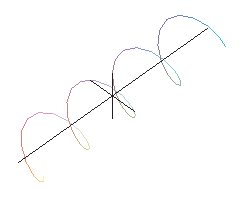
\includegraphics{pics/helix} \]

 Similarly, given a constant $c$, we can define
 \[ g\:\R^3\sm\{(0,0,0)\}\xra{}\R^3 \]
 by
 \[ g(x,y,z) =
     \left(\frac{-cx}{(x^2+y^2+z^2)^{3/2}},
           \frac{-cy}{(x^2+y^2+z^2)^{3/2}},
           \frac{-cz}{(x^2+y^2+z^2)^{3/2}}\right)
 \]
 This again has a physical interpretation: if there is a charged
 particle at the origin, and another charged particle at the point
 $(x,y,z)$, then the electric force felt by the second particle is
 $g(x,y,z)$. \qed
\end{example}

\begin{example}\bilabel{eg-mat-fun}
 There are many interesting and important functions involving
 matrices.  For example, consider the set $M$ of all $2\tm 2$
 matrices (with entries in $\R$).  An element of $M$ is a matrix, say
 $A=\bsm a&b\\c&d\esm$.  The determinant of such a matrix is the
 number $\det(A)=ad-bc\in\R$.  Thus, we have a rule that assigns an
 element $\det(A)\in\R$ to each element $A\in M$.  In other words, we
 have a function $\det\:M\xra{}\R$.
 
 Similarly, the \DEFN{trace} of a matrix $A=\bsm a&b\\c&d\esm$ is
 defined to be the number $\trc(A)=a+d$.  This gives another function
 $\trc\:M\xra{}\R$.

 Finally, the \DEFN{transpose} of a matrix $A$ as above is the matrix
 $A^T=\bsm a&c\\b&d\esm$.  We can define a function $\trans\:M\xra{}M$
 by $\trans(A)=A^T$. \qed
\end{example}

\begin{example}
 A function can be defined by a rule that is more complicated than a
 single formula.  For example, we can define a function
 $f\:\R\xra{}\Z$ by the following rule: $f(x)$ is the largest integer
 $n$ such that $n\leq x$.  (This is often written as $\text{floor}(x)$
 or $\lfloor x\rfloor$.)  For example, we have
 \begin{align*}
  f(-10.5) &= -11 \\
  f(-0.99) &= -1 \\
  f(-0.01) &= -1 \\
  f(\pi)   &= 3 \\
  f(9.999) &= 9.
 \end{align*}
 The graph is as follows:
 \begin{center}
  \begin{tikzpicture}[scale=0.5]
   \draw[->] (-5,0) -- (5,0);
   \draw[->] (0,-5) -- (0,5);
   \foreach \x in {-5 ,..., 5} \draw (\x,-0.1) -- (\x,0);
   \foreach \y in {-5 ,..., 5} \draw (-0.1,\y) -- (0,\y);
   \draw[red] (-5,-5) -- (-4,-5);
   \draw[dotted] (-4,-5) -- (-4,-4);
   \draw[red] (-4,-4) -- (-3,-4);
   \draw[dotted] (-3,-4) -- (-3,-3);
   \draw[red] (-3,-3) -- (-2,-3);
   \draw[dotted] (-2,-3) -- (-2,-2);
   \draw[red] (-2,-2) -- (-1,-2);
   \draw[dotted] (-1,-2) -- (-1,-1);
   \draw[red] (-1,-1) -- ( 0,-1);
   \draw[dotted] ( 0,-1) -- ( 0, 0);
   \draw[red] ( 0, 0) -- ( 1, 0);
   \draw[dotted] ( 1, 0) -- ( 1, 1);
   \draw[red] ( 1, 1) -- ( 2, 1);
   \draw[dotted] ( 2, 1) -- ( 2, 2);
   \draw[red] ( 2, 2) -- ( 3, 2);
   \draw[dotted] ( 3, 2) -- ( 3, 3);
   \draw[red] ( 3, 3) -- ( 4, 3);
   \draw[dotted] ( 4, 3) -- ( 4, 4);
   \draw[red] ( 4, 4) -- ( 5, 4);
   \fill (-5,-5) circle(0.05);
   \fill (-4,-4) circle(0.05);
   \fill (-3,-3) circle(0.05);
   \fill (-2,-2) circle(0.05);
   \fill (-1,-1) circle(0.05);
   \fill (0,0) circle(0.05);
   \fill (1,1) circle(0.05);
   \fill (2,2) circle(0.05);
   \fill (3,3) circle(0.05);
   \fill (4,4) circle(0.05);
  \end{tikzpicture}
 \end{center}
 Next, we can define $g\:\R\xra{}\R$ by
 \[ g(x) = (-1)^{\lfloor x\rfloor} = \begin{cases}
                          +1 & \text{ if $\lfloor x\rfloor$ is even } \\
                          -1 & \text{ if $\lfloor x\rfloor$ is odd. }
                         \end{cases}
 \]
 The graph of $g(x)$ is as follows:
 \begin{center}
  \begin{tikzpicture}[scale=0.6]
   \draw[->] (-5,0) -- (5,0);
   \draw[->] (0,-1.5) -- (0,1.5);
   \foreach \x in {-5 ,..., 5} \draw (\x,-0.1) -- (\x,0);
   \foreach \y in {-1 ,..., 1} \draw (-0.1,\y) -- (0,\y);
   \draw[red] (-5,-1) -- (-4,-1);
   \draw[dotted] (-4,-1) -- (-4,+1);
   \draw[red] (-4,+1) -- (-3,+1);
   \draw[dotted] (-3,+1) -- (-3,-1);
   \draw[red] (-3,-1) -- (-2,-1);
   \draw[dotted] (-2,-1) -- (-2,+1);
   \draw[red] (-2,+1) -- (-1,+1);
   \draw[dotted] (-1,+1) -- (-1,-1);
   \draw[red] (-1,-1) -- ( 0,-1);
   \draw[dotted] ( 0,-1) -- ( 0,+1);
   \draw[red] ( 0,+1) -- ( 1,+1);
   \draw[dotted] ( 1,+1) -- ( 1,-1);
   \draw[red] ( 1,-1) -- ( 2,-1);
   \draw[dotted] ( 2,-1) -- ( 2,+1);
   \draw[red] ( 2,+1) -- ( 3,+1);
   \draw[dotted] ( 3,+1) -- ( 3,-1);
   \draw[red] ( 3,-1) -- ( 4,-1);
   \draw[dotted] ( 4,-1) -- ( 4,+1);
   \draw[red] ( 4,+1) -- ( 5,+1);
   \fill (-5,-1) circle(0.05);
   \fill (-4,+1) circle(0.05);
   \fill (-3,-1) circle(0.05);
   \fill (-2,+1) circle(0.05);
   \fill (-1,-1) circle(0.05);
   \fill (0,+1) circle(0.05);
   \fill (1,-1) circle(0.05);
   \fill (2,+1) circle(0.05);
   \fill (3,-1) circle(0.05);
   \fill (4,+1) circle(0.05);
  \end{tikzpicture}
 \end{center}
 This is called a \DEFN{square wave} \mathworld{SquareWave}.  The CPU
 of a computer contains a ``clock circuit'', which generates a square
 wave, which is used to synchronise the actions of the various other
 parts of the chip.  The advertised speed of the chip is the frequency
 of this square wave; in a 2GHz chip, the voltage jumps up and down
 $2\tm 10^9$ times each second. \qed
\end{example}

\begin{example}\bilabel{eg-gray-code}
 If $A$ is a finite set, then one can specify a function $f\:A\xra{}B$
 simply by listing the values $f(a)$ for each element $a\in A$.  For
 example, we can define a function
 \[ \text{gray}\:\{0,1,\ldots,7\}\xra{}\{0,1,\ldots,7\} \]
 by the rule
 \[ \begin{array}{lll}
     \text{gray}(0) = 0 & \hspace{4em} & \text{gray}(4) = 6 \\
     \text{gray}(1) = 1 &              & \text{gray}(5) = 7 \\
     \text{gray}(2) = 3 &              & \text{gray}(6) = 5 \\
     \text{gray}(3) = 2 &              & \text{gray}(7) = 4
    \end{array}
 \]
 This table of values is in itself a complete and acceptable
 definition of the function.  There might or might not be some hidden
 reason why I chose to write down these particular values, but you do
 not need to know about that; the values themselves are all that you
 need in order to work with the function. \qed
\end{example}
\begin{background}
 This function is called the \DEFN{Gray code} \mathworld{GrayCode},
 and is not as random as it might seem.  It is easiest to understand
 if we rewrite the values in binary:
 \[ \begin{array}{lll}
     \text{gray}(0) = 000_2 & \hspace{4em} & \text{gray}(4) = 110_2 \\
     \text{gray}(1) = 001_2 &              & \text{gray}(5) = 111_2 \\
     \text{gray}(2) = 011_2 &              & \text{gray}(6) = 101_2 \\
     \text{gray}(3) = 010_2 &              & \text{gray}(7) = 100_2
    \end{array}
 \]
 The rule is as follows.  You start with $\text{gray}(0)=0$, and then
 define $\text{gray}(1)$ in terms of $\text{gray}(0)$, then define
 $\text{gray}(2)$ in terms of $\text{gray}(1)$, and so on.  To define
 $\text{gray}(n)$, you look at the binary expansion of
 $\text{gray}(n-1)$ and flip a single bit from $0$ to $1$ or
 vice-versa.  The bit to be flipped is taken as far to the right as
 possible, subject to the condition that $\text{gray}(n)$ must be
 different from $\text{gray}(0),\ldots,\text{gray}(n-1)$.  For
 example, to get $\text{gray}(4)$, we must flip one of the bits in
 $\text{gray}(3)=010_2$.  If we flip the rightmost bit, we get
 $011_2$, which has already occurred as $\text{gray}(2)$, so this is
 disallowed.  If we flip the middle bit, we get $000_2$, which has
 already occurred as $\text{gray}(0)$, which is again disallowed.  We
 thus have to flip the leftmost bit to get $\text{gray}(4)=110_2$.
 
 This function is useful if you want a digital system to measure the
 position of a wheel, for example.  The most obvious kind of
 measurement device risks being wildly wrong for an instant as it
 changes from one state to the next, but this problem is cured by the
 Gray code, because of the fact that $\text{gray}(n)$ and
 $\text{gray}(n-1)$ differ in only one place.
\end{background}

\begin{starex}\exlabel{ex_list_functions}
 Put $A=\{1,2,3\}$ and $B=\{\pi,-\pi\}$.
 \begin{itemize}
  \item[(a)] Write down a function $f_1\:A\xra{}B$.  Any function will
   do.
  \item[(b)] There are precisely eight different functions from $A$ to
   $B$.  Write down the other seven (you could call them
   $f_2$,\ldots,$f_8$).
  \item[(c)] Can you explain in a simple way why there are exactly
   eight different functions?
  \item[(d)] Suppose more generally that we have finite sets $C$ and
   $D$, with $|C|=n$ and $|D|=m$.  How many different functions are
   there from $C$ to $D$?
 \end{itemize}
\end{starex}
\begin{solution}
 \begin{itemize}
  \item[(a)] The simplest answer is the constant function defined by
   $f_1(1)=f_1(2)=f_1(3)=\pi$.
  \item[(b)] The full list is as follows:
   \[ \begin{array}{rlcrlcrl}
       f_1(1)&= \pi &\qquad& f_1(2)&= \pi &\qquad& f_1(3)&= \pi \\
       f_2(1)&= \pi &      & f_2(2)&= \pi &      & f_2(3)&=-\pi \\
       f_3(1)&= \pi &      & f_3(2)&=-\pi &      & f_3(3)&= \pi \\
       f_4(1)&= \pi &      & f_4(2)&=-\pi &      & f_4(3)&=-\pi \\
       f_5(1)&=-\pi &      & f_5(2)&= \pi &      & f_5(3)&= \pi \\
       f_6(1)&=-\pi &      & f_6(2)&= \pi &      & f_6(3)&=-\pi \\
       f_7(1)&=-\pi &      & f_7(2)&=-\pi &      & f_7(3)&= \pi \\
       f_8(1)&=-\pi &      & f_8(2)&=-\pi &      & f_8(3)&=-\pi
      \end{array}
   \]
  \item[(c)] There are $2$ ways to choose $f(1)$, then two ways to
   choose $f(2)$, then two ways to choose $f(3)$, making
   $2\tm 2\tm 2=8$ ways to choose a function $f\:A\xra{}B$
   altogether.
  \item[(d)] As $|C|=n$, we can list the elements of $C$ as
   $\{c_1,\ldots,c_n\}$ say (without any repetitions).  We then have
   $m$ ways to choose $f(c_i)$ for each $i$, making
   $m\tm\ldots\tm m=m^n$ ways to choose a function $f\:C\xra{}D$.
   Thus, there are precisely $m^n$ different functions from $C$ to
   $D$.
 \end{itemize}
\end{solution}


\section{The range}
\label{sec-range}

Given a function $f\:A\xra{}B$, the \DEFN{range} of $f$ is the set of
all $b\in B$ that can be written in the form $b=f(a)$ for some 
$a\in A$.  We write $\PURPLE{\range(f)}$ or $\PURPLE{f(A)}$ for this
set. 

If $A$ and $B$ are intervals in $\R$, then we can display this
graphically.  We draw the graph of $f$ (with the $x$-axis covering
only the set $A$), then squash the graph sideways onto the $y$-axis.
The resulting set on the $y$-axis is the range of $f$.
\begin{example}
 Consider the function $f\:[-2,2]\xra{}\R$ given by
 $f(x)=(x^2-1)^2+1=x^4-2x^2+2$.  The graph is as follows:
 \begin{center}
  \begin{tikzpicture}[xscale=1.6,yscale=0.4]
   \def\ff(#1){{(#1*#1*#1*#1-2*#1*#1+2)}}
   \def\gg(#1){sqrt(sqrt(#1 - 1)+1)}
   \draw[->] (-2.2,0) -- (2.2,0);
   \draw[->] (0,0) -- (0,13);
   \foreach \x in {-2,-1,0,1,2} \draw (\x,-0.5) -- (\x,0);
   \foreach \y in {0 ,..., 12} \draw (-0.1,\y) -- (0,\y);
   \draw[dotted] (-2,0) -- (-2,10);
   \draw[dotted] (+2,0) -- (+2,10);
   \draw [red,domain=-2:2,samples=200,variable=\x] plot(\x,{\ff(\x)});
   \foreach \y in {1.0,1.5,...,10} {
    \draw[olivegreen] ({-\gg(\y)},\y) -- ({\gg(\y)},\y);
   }
   \draw[ultra thick,olivegreen] (0,1) -- (0,10);
   \draw (-2,-1) node[anchor=north] {$-2$};
   \draw (+2,-1) node[anchor=north] {$+2$};
   \fill (0,1) circle(0.05);
   \fill (0,10) circle(0.05);
   \draw (-0.1,1.0) node[anchor=north east] {$1$};
   \draw (-0.1,10.1) node[anchor=south east] {$10$};
  \end{tikzpicture}
 \end{center}
 As $x$ runs from $-2$ to $2$, the function $f(x)$ runs from $10$ down
 to $1$, then back up to $2$, back down to $1$, and then back up to
 $10$.  It is thus clear that the range is $[1,10]$. \qed
\end{example}
\begin{warning}
 Please avoid the \RED{\textbf{standard mistake}}.  Given a function
 $f\:[a,b]\xra{}\R$, you \RED{\textbf{cannot}} find the range by working
 out $f(a)$ and $f(b)$ and saying that the range is $[f(a),f(b)]$.  In
 the above example, we have a function $f\:[-2,+2]\xra{}\R$ with
 $f(-2)=f(2)=10$.  The incorrect rule would say that the range is the
 interval $[10,10]$, or in other words the set $\{10\}$, which is
 obviously wrong.
\end{warning}

\begin{example}
 Consider $f\:[0,\infty)\xra{}[0,\infty)$ given by $f(a)=a+1$ (so
 $A=B=[0,\infty)$).  It is easy to see that the range is
 $[1,\infty)$. \qed 
\end{example}

\begin{exercise}\exlabel{ex_quad_range}
 Let $a$ and $b$ be strictly positive constants, and define
 $f\:[0,2a]\xra{}\R$ by $f(x)=(x-a)^2+b$.  What is the range of $f$?
 (You may want to choose some random values for $a$ and $b$, and sketch
 the graph, to see what is going on.  However, your final answer should
 be given in a way that works for all $a$ and $b$.)
\end{exercise}
\begin{solution}
 The picture is as follows:
 \begin{center}
  \begin{tikzpicture}[scale=2.5]
   \draw[->] (-0.2,0) -- (2,0);
   \draw[->] (0,0) -- (0,2.2);
   \draw (2,0) -- (2,2.1);
   \begin{scope}[draw=olivegreen]
    \draw ( 1,      1.0) -- (0,1.0);
    \draw ( 1.31623,1.1) -- (0,1.1);
    \draw ( 1.44721,1.2) -- (0,1.2);
    \draw ( 1.54772,1.3) -- (0,1.3);
    \draw ( 1.63246,1.4) -- (0,1.4);
    \draw ( 1.70711,1.5) -- (0,1.5);
    \draw ( 1.7746 ,1.6) -- (0,1.6);
    \draw ( 1.83666,1.7) -- (0,1.7);
    \draw ( 1.89443,1.8) -- (0,1.8);
    \draw ( 1.94868,1.9) -- (0,1.9);
    \draw ( 2.     ,2.0) -- (0,2.0);
   \end{scope}
   \draw[red,domain=0:2,samples=100,variable=\x] plot(\x,{(\x-1)*(\x-1)+1});
   \draw (0,-0.1) node[anchor=north] {$\scriptstyle 0$};
   \draw (1,-0.1) node[anchor=north] {$\scriptstyle a$};
   \draw (2,-0.1) node[anchor=north] {$\scriptstyle 2a$};
   \draw (-0.1,1) node[anchor=east] {$\scriptstyle b$};
   \draw (-0.1,2) node[anchor=east] {$\scriptstyle b+a^2$};
  \end{tikzpicture}
 \end{center}
 As $x$ runs from $0$ to $2a$, the function $f(x)$ runs from $b+a^2$
 down to $b$ and then up to $b+a^2$ again.  This makes it clear that
 the range is $[b,b+a^2]$.
\end{solution}
\begin{exercise}\exlabel{ex_trig_range}
 Define $f\:[\pi/6,7\pi/6]\xra{}\R$ by $f(x)=\sin(x)$.  What is the
 range of $f$?
\end{exercise}
\begin{solution}
 The graph is as follows:
 \begin{center}
  \begin{tikzpicture}[xscale=0.7,yscale=3]
   \draw[->] (0,0) -- (13,0);
   \draw[->] (0,-1.2) -- (0,1.2);
   \draw[yellow,domain=0:1,samples=20,variable=\x] plot(\x,{sin(30*\x)});
   \draw[red   ,domain=1:7,samples=120,variable=\x] plot(\x,{sin(30*\x)});
   \draw[yellow,domain=7:12,samples=100,variable=\x] plot(\x,{sin(30*\x)});
   \begin{scope}[draw=olivegreen]
    \draw (7., -0.5) -- (0,-0.5);
    \draw (6.78594, -0.4) -- (0,-0.4);
    \draw (6.58192, -0.3) -- (0,-0.3);
    \draw (6.38457, -0.2) -- (0,-0.2);
    \draw (6.19131, -0.1) -- (0,-0.1);
    \draw (6., 0.) -- (0,0.);
    \draw (5.80869, 0.1) -- (0,0.1);
    \draw (5.61543, 0.2) -- (0,0.2);
    \draw (5.41808, 0.3) -- (0,0.3);
    \draw (5.21406, 0.4) -- (0,0.4);
    \draw (5., 0.5) -- (0,0.5);
    \draw (4.771, 0.6) -- (0,0.6);
    \draw (4.5191, 0.7) -- (0,0.7);
    \draw (4.229, 0.8) -- (0,0.8);
    \draw (3.8614,  0.9) -- (0, 0.9);
    \draw (3., 1.) -- (0,1.);
   \end{scope}
   \draw[blue] (1,0) -- (1,.5);
   \draw[blue] (7,0) -- (7,-.5);
   \draw (-0.1,-0.5) node[anchor=east] {$\scriptstyle -1/2$};
   \draw (-0.1, 0.0) node[anchor=east] {$\scriptstyle 0$};
   \draw (-0.1, 0.5) node[anchor=east] {$\scriptstyle 1/2$};
   \draw (-0.1, 1.0) node[anchor=east] {$\scriptstyle 1$};
  \end{tikzpicture}
 \end{center}
 As $x$ runs from $\pi/6$ to $7\pi/6$, the function $f(x)$ runs from
 $1/2$ up to $1$ and then down to $-1/2$.  This shows that the range
 is $[-1/2,1]$.
\end{solution}

\begin{sstarex}\exlabel{ex_circle_range}
 Define $f\:\R\xra{}\R^2$ by
 $f(t)=(\frac{1-t^2}{1+t^2},\frac{2t}{1+t^2})$.  (Note that this is
 meaningful for all $t$, because $1+t^2$ is never zero.)  What is the
 range of $f$?  (Hint: An earlier exercise almost gives the answer;
 you should at least get that far.  One small detail needs to be
 adjusted, and then everything needs to be properly justified, which
 is quite intricate.)
\end{sstarex}
\begin{solution}
 Let $C$ be the unit circle, or in other words
 \[ C = \{(x,y)\in\R^2 \st x^2+y^2 = 1\}. \]
 We saw in \exref{ex_circle_rational} that
 \[ \left(\frac{1-t^2}{1+t^2}\right)^2 +
    \left(\frac{2t}{1+t^2}\right)^2 = 1,
 \]
 so that $f(t)$ always lies in $C$, so $\range(f)\sse C$.  The obvious
 guess, which you could support with Maple or a graphing calculator,
 is that $\range(f)=C$.  However, this is not quite right.
 
 Put $p=(-1,0)\in C$; I claim that $f(t)$ is never equal to $p$, so
 that $p$ does \EMPH{not} lie in $\range(f)$ .  Indeed, if $f(t)$ were
 equal to $p$ we would have $(1-t^2)/(1+t^2)=-1$ and $2t/(1+t^2)=0$.
 Multiplying the first equation by $1+t^2$ and then adding $t^2$ to
 both sides, we get $1=-1$, which is impossible.  Thus, we cannot have
 $f(t)=p$, so the range of $f$ is not all of $C$.  More precisely, if
 we put
 \[ C'=C\sm\{p\} = \{(x,y)\in C \st x>-1\}, \]
 we have shown that the range of $f$ is a subset of $C'$.  I claim
 that the range is actually all of $C'$.  Indeed, suppose we have a
 point $(x,y)\in C'$, so that $x^2+y^2=1$ and $x>-1$.  This means that
 $1+x$ is nonzero, so we can meaningfully put $t=y/(1+x)$.  Using the
 equation $y^2=1-x^2=(1-x)(1+x)$, we see that
 \begin{align*}
  t^2 &= \frac{y^2}{(1+x)^2} = \frac{(1-x)(1+x)}{(1+x)^2}
          = \frac{1-x}{1+x} \\
  1+t^2 &= 1 + \frac{1-x}{1+x} = \frac{2}{1+x} \\
  1-t^2 &= 1 - \frac{1-x}{1+x} = \frac{2x}{1+x} \\
  \frac{1-t^2}{1+t^2} &= \frac{2x}{1+x}/\frac{2}{1+x} = x \\
  \frac{2t}{1+x}      &= \frac{2y}{1+x}/\frac{2}{1+x} = y \\
  f(t) &= \left(\frac{1-t^2}{1+t^2},\frac{2t}{1+t^2}\right)
          = (x,y).
 \end{align*}
 This shows that $(x,y)$ lies in the range of $f$, for any point
 $(x,y)$ in $C'$, so $C'\sse\range(f)$.  We have already seen that
 $\range(f)\sse C'$, so in fact $\range(f)=C'$ as claimed.
\end{solution}

\begin{sstarex}\exlabel{ex_parabolic_region}
 Define a map $f\:\R^2\xra{}\R^2$ by
 \[ f(u,v) = (u+v,4uv). \]
 Consider the set
 \[ Q = \{(x,y)\in\R^2\st y \leq x^2\}, \]
 or in other words, the region below the parabola $y=x^2$:
 \begin{center}
  \begin{tikzpicture}[xscale=2,yscale=0.8]
   \fill[red   ,domain=-2:2,samples=100,variable=\x] plot(\x,{\x*\x}) -- (2,-4) -- (-2,-4) -- cycle;
   \draw[->] (-2.3,0) -- (2.3,0);
   \draw[->] (0,-4.5) -- (0,4.5);
   \foreach \x in {-2 ,..., 2} \draw (\x,-0.1) -- (\x,0);
   \foreach \y in {-4 ,..., 4} \draw (-0.1,\y) -- (0,\y);
  \end{tikzpicture}
 \end{center}
 Show that $Q$ is the range of $f$.
\end{sstarex}
\begin{solution}
 We must first show that $\range(f)\sse Q$, or in other words that
 $(u+v,4uv)$ always lies in $Q$, or in other words that
 $4uv\leq(u+v)^2$ for all real numbers $u$ and $v$.  To see this,
 note that
 \begin{align*}
  (u+v)^2 - 4uv &= u^2 + 2uv + v^2 - 4uv \\
                &= u^2 - 2uv + v^2 = (u-v)^2 \geq 0,
 \end{align*}
 so $(u+v)^2\geq 4uv$ as claimed.

 Secondly, we must show that $Q\sse\range(f)$.  Equivalently, given a
 point $(x,y)\in\R^2$ with $y\leq x^2$, we must find a point
 $(u,v)\in\R^2$ such that $u+v=x$ and $4uv=y$.  For this, we note that
 $x^2-y\geq 0$ by assumption, so it is meaningful to put
 $r=\sqrt{x^2-y}$.  We then put $u=(x+r)/2$ and $v=(x-r)/2$.  It is
 clear that $u+v=x$, and
 \[ 4uv = (x+r)(x-r) = x^2 - r^2 = x^2 - (x^2 - y) = y, \]
 so
 \[ f(u,v) = (u+v,4uv) = (x,y) \]
 as required.
\end{solution}

\begin{starex}\exlabel{ex_stretch}
 Show that there are well-defined functions $f\:(0,\infty)\xra{}(0,1)$
 and $g\:(0,1)\xra{}(0,\infty)$, given by
 \begin{align*}
  f(x) &= x/\sqrt{1+x^2} \\
  g(y) &= y/\sqrt{1-y^2}.
 \end{align*}
 Show that $f$ and $g$ are inverse to each other.  (First just do the
 algebra to check that $f(g(x))=x$ and $g(f(y))=y$; then give a
 careful argument to show that everything is well-defined and that
 there are no problems with signs.)
\end{starex}
\begin{solution}
 I first claim that we can define a function
 $f\:(0,\infty)\xra{}(0,1)$ by $f(x)=x/\sqrt{1+x^2}$.  Indeed, when
 $x>0$ we certainly have $1+x^2>0$ so $\sqrt{1+x^2}$ is defined and is
 nonzero, so $f(x)=x/\sqrt{1+x^2}$ is a well-defined number.  However,
 if we want to consider $f$ as a function from $(0,\infty)$ to
 $(0,1)$, we need to show that $f(x)$ always lies in $(0,1)$, or
 equivalently that $0<x/\sqrt{1+x^2}<1$ for all $x>0$.  For this, we
 note that
 \[ 0< x^2 < 1+x^2. \]
 Everything here is positive, so it is legitimate to take square
 roots, and we deduce that
 \[ 0< x < \sqrt{1+x^2}. \]
 As $\sqrt{1+x^2}>0$, it is legitimate to divide by this quantity
 without changing the inequality signs, and we deduce that
 \[ 0 < x/\sqrt{1+x^2} < 1, \]
 as required.

 I now claim that we can define a function $g\:(0,1)\xra{}(0,\infty)$
 by $g(y)=y/\sqrt{1-y^2}$.  Indeed, if $y\in(0,1)$ then $1-y^2>0$, so
 $\sqrt{1-y^2}$ is defined and is strictly positive, so
 $y/\sqrt{1-y^2}$ is also defined and strictly positive.

 Finally, I claim that $f$ and $g$ are inverses of each other, or in
 other words that $f(g(y))=y$ for all $y\in(0,1)$, and $g(f(x))=x$ for
 all $x\in(0,\infty)$.  To see this, note that
 \begin{align*}
  1 + g(y)^2 &= 1 + \frac{y^2}{1-y^2} = \frac{1}{1-y^2} \\
  \sqrt{1+g(y)^2} &= 1/\sqrt{1-y^2} \\
  f(g(y)) &= \frac{g(y)}{\sqrt{1+g(y)^2}}
           = \frac{y}{\sqrt{1-y^2}}/ \frac{1}{\sqrt{1-y^2}} = y.
 \end{align*}
 The proof that $g(f(x))=x$ is similar.
\end{solution}


\section{Composition}
\label{sec-composition}

\begin{definition}
 Suppose we have functions $f\:A\xra{}B$ and $g\:B\xra{}C$.  We then
 define a function \DEFN{$h=g\circ f\:A\xra{}C$} by $h(a)=g(f(a))$.
 \begin{center}
  \begin{tikzpicture}
   \draw (-4, 0) node {$A$};
   \draw (0, 0) node {$B$};
   \draw (4, 0) node {$C$} ;
   \draw (-4,-1) node {$a$};
   \draw (0,-1) node {$f(a)$};
   \draw (4,-1) node {$g(f(a))$} ;
   \draw[->] (-3.5, 0) -- (-0.5, 0);
   \draw[->] (+0.5, 0) -- (+3.5, 0);
   \draw (-2,.3) node {$f$};
   \draw (+2,.3) node {$g$};
   \draw[red,->] (-3.5,-1) -- (-0.7,-1); 
   \draw[red] (-3.5,-1.1) -- (-3.5,-0.9);
   \draw[red,->] (+0.7,-1) -- (+2.9,-1);
   \draw[red] (+0.7,-1.1) -- (+0.7,-0.9);
  \end{tikzpicture}
 \end{center}
 This is called the \DEFN{composite} of $f$ and $g$.
\end{definition}

\begin{example}
 Consider $f,g,h\:\R\xra{}\R$ given by $f(x)=x+1$ and $g(x)=2x$.  I
 claim that $f\circ f\circ g=g\circ f$.  Indeed, we have
 \begin{align*}
  (f\circ f\circ g)(x) &=
   f(f(g(x))) = f(f(2x)) = f(2x+1) = 2x+2 \\
  (g\circ f)(x) &= g(f(x))=g(x+1)= 2(x+1)= 2x+2.
 \end{align*}
 This holds for all $x$, so $f\circ f\circ g=g\circ f$. \qed
\end{example}
\begin{example}
 Consider the functions
 $\R\xra{f}\R^3\xra{g}\R$ and $\R\xra{h}\R$ given by
 \begin{align*}
  f(t)     &= (1,t,t^2) \\
  g(x,y,z) &= x+2y+z \\
  h(t)     &= (1+t)^2.
 \end{align*}
 I claim that $g\circ f=h$.  Indeed, we have
 \begin{align*}
  (g\circ f)(t) &= g(f(t)) \\
                &= g(1,t,t^2) \\
                &= 1 + 2t + t^2 \\
                &= (1+t)^2 = h(t).
 \end{align*}
 This holds for all $t\in\R$, so $h=g\circ f$. \qed
\end{example}

\begin{exercise}\exlabel{ex_trace_comp}
 Let $M$ be the set of all $2\tm 2$ matrices.  (Matrices will be
 explained in \autoref{chap-mat}; you should ignore this exercise if
 you are not already familiar with them.)

 Define functions $\R\xra{f}M\xra{g}M\xra{h}\R$ by 
 \begin{align*}
  f(t) &= \bsm 1 & t \\ 0 & 1 \esm \\
  g(A) &= AA^T \\
  h(B) &= \trc(B).
 \end{align*}
 What are the domain and codomain of the function $k=h\circ g\circ f$?
 What is the formula for this function?
\end{exercise}
\begin{solution}
 The composite $k=h\circ g\circ f$ is a function from $\R$ to $\R$, so
 $\text{domain}(k)=\text{codomain}(k)=\R$.  The formulae are as
 follows: 
 \begin{align*}
  (g\circ f)(t) &= g(f(t)) = g\bbm 1 & t \\ 0 & 1\ebm \\
    &= \bbm 1 & t \\ 0 & 1 \ebm \bbm 1 & t \\ 0 & 1 \ebm^T \\
    &= \bbm 1 & t \\ 0 & 1 \ebm \bbm 1 & 0 \\ t & 1 \ebm \\
    &= \bbm 1+t^2 & t \\ t & 1 \ebm \\
  h\bbm p & q \\ r & s \ebm &= p+s \\
  k(t) &= h(g(f(t))) = h\bbm 1+t^2 & t \\ t & 1 \ebm 
        = (1+t^2)+1 = 2+t^2.
 \end{align*}
\end{solution}
\begin{exercise}\exlabel{ex_mobius_six}
 Put $A=\R\sm\{0,1\}$, and define $f,g,h\:A\xra{}A$ by 
 \begin{align*}
  f(x) &= 1-x \\
  g(x) &= 1/x \\
  h(x) &= g(f(x)).
 \end{align*}
 Check that this is all meaningful, and simplify
 $(h\circ h)(x)$ and $(h\circ h\circ h)(x)$.
\end{exercise}
\begin{solution}
 First, if $x\in\R$ and $x\neq 0,1$ then $1-x$ is again a real number
 and $1-x\neq 0,1$.  This means that the equation $f(x)=1-x$ really
 does give a function $f\:A\xra{}A$.

 Similarly, if $x\in\R$ and $x\neq 0,1$ then $1/x$ is a well-defined
 real number (because we have excluded the problematic case where
 $x=0$) and we see easily that $1/x\neq 0,1$.  Thus, the rule
 $g(x)=1/x$ defines another function $g\:A\xra{}A$.  It follows in
 turn that the rule $h(x)=g(f(x))$ defines a well-defined function
 $g\:A\xra{}A$. 

 Next, we have
 \begin{align*}
  h(x)&= 1-1/x = (x-1)/x \\
  (h\circ h)(x) &= h(\frac{x-1}{x}) = 1 - \frac{x}{x-1} = \frac{1}{1-x} \\
  (h\circ h\circ h)(x) &= h\left(\frac{1}{1-x}\right) = 
                          1 - \frac{1-x}{1} = x.
 \end{align*}
\end{solution}
\begin{exercise}\exlabel{ex_mobius_factor}
 Given numbers $\lm$ and $\mu$, we put
 \begin{align*}
  f_\lm(t) &= t+\lm \\
  g_\mu(t) &= \mu t \\
  h(t)     &= 1/t.
 \end{align*}
 Let $a,b,c$ and $d$ be numbers with $c\neq 0$ and $ad\neq bc$, and
 put 
 \[ k = f_{a/c}\circ h \circ g_{c^2/(bc-ad)} \circ f_{d/c}. \]
 Simplify $k(t)$.  (You may wish to consider the intermediate
 variables $u=f_{d/c}(t)$, $v=g_{c^2/(bc-ad)}(u)$ and $w=h(v)$.)

 This is relevant to the theory of \DEFN{M\"obius transformations}
 (otherwise known as \DEFN{linear fractional transformations})
 \mathworld{LinearFractionalTransformation}.  You need not discuss the
 domain of definition of any of the functions used.
\end{exercise}
\begin{solution}
 We must find $k(t)=f_{a/c}(h(g_{c^2/(bc-ad)}(f_{d/c}(t))))$.  We can
 rephrase this as follows: we put $u=f_{d/c}(t)$ and
 $v=g_{c^2/(bc-ad)}(u)$ and $w=h(v)$ and $x=f_{a/c}(w)$, so $k(t)=x$.
 \begin{align*}
  u &= t+\frac{d}{c} = \frac{ct+d}{c} \\
  v &= \frac{c^2}{bc-ad}u = \frac{c^2}{bc-ad} \frac{ct+d}{c}
       = \frac{c(ct+d)}{bc-ad} \\
  w &= h(u) = 1/u = \frac{bc-ad}{c(ct+d)} \\
  x &= w + \frac{a}{c} =
       \frac{bc-ad}{c(ct+d)} + \frac{a(ct+d)}{c(ct+d)} \\
    &= \frac{b\OLIVEGREEN{c}-\RED{ad}+a\OLIVEGREEN{c}t+\RED{ad}}
            {\OLIVEGREEN{c}(ct+d)} = 
       \frac{at+b}{ct+d}
 \end{align*}
 The conclusion is that $k(t)=(at+b)/(ct+d)$.
\end{solution}

\begin{exercise}\exlabel{ex_refl_comp}
 Define $f,g\:\R^2\xra{}\R^2$ by 
 \begin{align*}
  f(x,y) &= (1-y,1-x) \\
  g(x,y) &= (-1-y,-1-x).
 \end{align*}
 Find $f\circ f$, $f\circ g$, $g\circ f$ and $g\circ g$.
\end{exercise}
\begin{solution}
 \begin{align*}
  (f\circ f)(x,y) &= f(1-y,1-x) = (1-(1-x),1-(1-y)) = (x,y) \\
  (f\circ g)(x,y) &= f(-1-y,-1-x) = (1-(-1-x),1-(-1-y)) = (x+2,y+2) \\
  (g\circ f)(x,y) &= g(1-y,1-x) = (-1-(1-x),-1-(1-y)) = (x-2,y-2) \\
  (g\circ g)(x,y) &= g(-1-y,-1-x) = (-1-(-1-x),-1-(-1-y)) = (x,y).
 \end{align*}
 Geometrically, it works out that $f(x,y)$ is the reflection of $x$
 across the line $x+y=1$, and $g(x,y)$ is the reflection of $(x,y)$
 across the line $x+y=-1$.  It is also possible to work out the
 composites from this information.  For example, if you reflect twice
 in succession across the same line then that is the same as doing
 nothing, which explains why $(f\circ f)(x,y)=(x,y)=(g\circ g)(x,y)$.
\end{solution}
\begin{exercise}\exlabel{ex_rot_power}
 Put $A=\{1,2,3,4\}$, and define $f\:A\xra{}A$ by 
 $f(1)=2$, $f(2)=3$, $f(3)=4$ and $f(4)=1$.  Describe the function 
 $g=f\circ f\circ f\:A\xra{}A$.
\end{exercise}
\begin{solution}
 We can list the values as follows:
 \[ \renewcommand{\arraystretch}{1.5}
   \begin{array}{|r||c|c|c|c|}
    \hline
     n                 & 1 & 2 & 3 & 4 \\ 
    \hline
     f(n)              & 2 & 3 & 4 & 1 \\
     f(f(n))           & 3 & 4 & 1 & 2 \\
     g(n) = f(f(f(n))) & 4 & 1 & 2 & 3 \\
    \hline
   \end{array}
 \]
 This can also be displayed as follows:
 \begin{center}
  \begin{tikzpicture}[thick,xscale=2]
   \begin{scope}[draw=red,text=red]
    \draw (0,-1) node {$1$};
    \draw[->] (0.1,-1.1) -- (0.9,-1.9);
    \draw (1,-2) node {$2$};
    \draw[->] (1.1,-2.1) -- (1.9,-2.9);
    \draw (2,-3) node {$3$};
    \draw[->] (2.1,-3.1) -- (2.9,-3.9);
    \draw (3,-4) node {$4$};
   \end{scope}
   \begin{scope}[draw=blue,text=blue]
    \draw (0,-2) node {$2$};
    \draw[->] (0.1,-2.1) -- (0.9,-2.9);
    \draw (1,-3) node {$3$};
    \draw[->] (1.1,-3.1) -- (1.9,-3.9);
    \draw (2,-4) node {$4$};
    \draw (2.10,-3.70) -- (2.20,-3.40);
    \draw (2.30,-3.10) -- (2.45,-2.65);
    \draw (2.55,-2.35) -- (2.70,-1.90);
    \draw[->] (2.80,-1.60) -- (2.90,-1.30);
    \draw (3,-1) node {$1$};
   \end{scope}
   \begin{scope}[draw=magenta,text=magenta]
    \draw (0,-3) node {$3$};
    \draw[->] (0.1,-3.1) -- (0.9,-3.9);
    \draw (1,-4) node {$4$};
    \draw (1.10,-3.70) -- (1.20,-3.40);
    \draw (1.30,-3.10) -- (1.45,-2.65);
    \draw (1.55,-2.35) -- (1.70,-1.90);
    \draw[->] (1.80,-1.60) -- (1.90,-1.30);
    \draw (2,-1) node {$1$};
    \draw[->] (2.1,-1.1) -- (2.9,-1.9);
    \draw (3,-2) node {$2$};
   \end{scope}
   \begin{scope}[draw=olivegreen,text=olivegreen]
    \draw (0,-4) node {$4$};
    \draw (0.10,-3.70) -- (0.20,-3.40);
    \draw (0.30,-3.10) -- (0.45,-2.65);
    \draw (0.55,-2.35) -- (0.70,-1.90);
    \draw[->] (0.80,-1.60) -- (0.90,-1.30);
    \draw (1,-1) node {$1$};
    \draw[->] (1.1,-1.1) -- (1.9,-1.9);
    \draw (2,-2) node {$2$};
    \draw[->] (2.1,-2.1) -- (2.9,-2.9);
    \draw (3,-3) node {$3$};
   \end{scope}
  \end{tikzpicture}
 \end{center}
 The conclusion is that $g(1)=4$, $g(2)=1$, $g(3)=2$ and $g(4)=3$.
\end{solution}
\begin{starex}\exlabel{ex_logistic}
 There are plausible (but crude) models of population growth
 \mathworld{LogisticMap} that look like this: if there are $x$ beasts
 per square metre this year, then there will be $f(x)$ beasts per square
 metre next year, where $f(x)=3x(1-x)$.  (The idea is that if the
 population is small then it will grow rapidly, but if the population
 approaches one beast per square metre then many will starve
 through overcrowding and the population will plummet.)  The population
 in two years' time will then be $f^2(x)=f(f(x))$, in three years' time
 it will be $f^3(x)=f(f(f(x)))$ and so on.
 \begin{itemize}
  \item Expand out $f(x)$.
  \item Expand out $f(f(x))$.
  \item Use Maple to expand out $f^3(x)$.
  \item How many terms are there in each of the answers you have
   obtained?  What are the first and last terms?  What do you get if
   you factor the coefficients in the first and last terms?
  \item Can you guess how many terms there will be in $f^{10}(x)$?
   What will the first and last terms be?
 \end{itemize}
 This exercise should convince you that explicit calculation of
 $f^{10}(x)$ would give an expression that is much to large and
 unwieldy to tell us anything very useful.  Nonetheless, there is an
 elaborate and interesting theory of models of this type, which tells
 us a great deal about $f^n(x)$ for all $n$, by more indirect
 methods.  Some of these ideas are covered in \PMA{324} (Chaos) and
 \PMA{443} (Fractals).
\end{starex}
\begin{solution}
 We have
 \begin{align*}
  f(x)   &= 3x - 3x^2 \\
  f^2(x) &= 3f(x) - 3f(x)^2 \\
         &= 3(3x-3x^2) - 3(3x-3x^2)^2 \\
         &= 9x - 9x^2 - 3(9x^2 - 18 x^3 + 9x^4) \\
         &= 9x - 36x^2 + 54 x^3 - 27 x^4 \\
         &= 3^2x - \cdots - 3^3 x^4 \\
  f^3(x) &= 27x-351x^2+2106x^3-6885x^4+
            13122*x^5-14580x^6+8748x^7-2187x^8 \\
         &= 3^3x - \cdots - 3^7 x^8
 \end{align*}
 The general rule is that $f^n(x)$ has $2^n$ terms, starting with
 $3^nx$, and ending with $-3^{2^n-1}x^{2^n}$.  (Can you explain why?)
 In particular,
 \[ f^{10}(x) = 3^{10}x - \cdots - 3^{1023}x^{1024}. \]
\end{solution}


\section{Inverse functions}
\label{sec-func-inv}

\begin{definition}
 Suppose we have a function $f\:A\xra{}B$.  An \DEFN{inverse} for $f$
 is a function $g\:B\xra{}A$ such that $g(f(a))=a$ for \EMPH{all}
 $a\in A$, \EMPH{and} $f(g(b))=b$ for \EMPH{all} $b\in B$.  Once we
 have shown that $g$ has these properties, we sometimes use the
 notation \DEFN{$f^{-1}(b)$} for $g(b)$.
\end{definition}
\begin{example}\bilabel{eg-affine-inverse}
 Define $f,g\:\R\xra{}\R$ by $f(x)=2x+1$ and $g(y)=(y-1)/2$.  Then
 \begin{align*}
  g(f(x)) &= g(2x+1) = ((2x+1)-1)/2 = x \\
  f(g(y)) &= f((y-1)/2) = 2(y-1)/2 + 1 = y.
 \end{align*}
 These equations hold for all $x$ and $y$ in $\R$, so $g$ is inverse
 to $f$. \qed
\end{example}
\begin{example}\bilabel{eg-exp-inv}
 As discussed in more detail in \autoref{sec-explog}, the function
 $\exp\:\R\xra{}(0,\infty)$ is inverse to the function
 $\log\:(0,\infty)\xra{}\R$.  \qed
\end{example}
\begin{warning}
 It is a \RED{\textbf{standard mistake}} to confuse $f^{-1}(x)$ with
 the function $f(x)^{-1}=1/f(x)$.  These two functions are completely
 different.  For example, $\exp^{-1}(e)=\log(e)=1$, but
 $\exp(e)^{-1}=e^{-e}\approx 0.065988$.
\end{warning}
\begin{warning}
 Another \RED{\textbf{standard mistake}} is to check only one of the
 two equations $g(f(x))=x$ and $f(g(y))=y$.  \EMPH{Both} of these must
 be true for $g$ to be inverse to $f$.
\end{warning}
\begin{example}\bilabel{eg-finite-inverse}
 Put $A=\{0,1,2,3\}$ and $B=\{1,2,4,8\}$, and define functions
 $A\xra{f}B\xra{g}A$ as follows:
 \[ \renewcommand{\arraystretch}{1.5}
  \begin{array}{|r|c|c|c|c|}
   \hline
    n    & 0 & 1 & 2 & 3 \\
   \hline
    f(n) & 8 & 4 & 2 & 1 \\ 
   \hline\hline
    m    & 1 & 2 & 4 & 8 \\
   \hline
    g(m) & 3 & 2 & 1 & 0 \\
   \hline
  \end{array}
 \]
 We then have 
 \[ \renewcommand{\arraystretch}{1.5}
  \begin{array}{rlcrl}
   g(f(0)) &= g(8) = 0 & \qquad & f(g(1)) &= f(3) = 1 \\
   g(f(1)) &= g(4) = 1 & \qquad & f(g(2)) &= f(2) = 2 \\
   g(f(2)) &= g(2) = 2 & \qquad & f(g(4)) &= f(1) = 4 \\
   g(f(3)) &= g(1) = 3 & \qquad & f(g(8)) &= f(0) = 8.
  \end{array}
 \]
 Thus $g(f(n))=n$ for all $n\in A$ and $f(g(m))=m$ for all $m\in B$,
 so $g$ is inverse to $f$. \qed
\end{example}
\begin{example}\bilabel{eg-sqrt-inverse}
 Define $f\:\R\xra{}[0,\infty)$ by $f(x)=x^2$.  Next, define
 $g\:[0,\infty)\xra{}\R$ by 
 \[ g(y) = \sqrt{y} = \text{ the nonnegative square root of } y. \]
 It is natural to think that $g$ is inverse to $f$, but this is not
 quite right.  To see this, note that $f(-1)=(-1)^2=1$, so
 $g(f(-1))=g(1)=\sqrt{1}=1$, so $g(f(-1))\neq -1$.
 
 This can be fixed if we specify the domains and codomains of our
 functions differently.  Put $A=[0,\infty)$ and let $f_0$ be the
 function \EMPH{from $A$ to $A$} with formula $f_0(x)=x^2$, and let
 $g_0$ be the function \EMPH{from $A$ to $A$} with formula
 $g_0(y)=\sqrt{y}$.  As explained in
 \hyperlink{rem-fn-pitfalls}{Remark~\ref{rem-fn-pitfalls}(d)}, $f_0$
 and $g_0$ are, strictly speaking, different functions from $f$ and
 $g$.  For any $x\in A$ we have $x\geq 0$ and so
 $x=\sqrt{x^2}=(\sqrt{x})^2$, or in other words
 $x=g_0(f_0(x))=f_0(g_0(x))$.  This means that $g_0$ is inverse to
 $f_0$, even though $g$ is not inverse to $f$. \qed
\end{example}

Many functions do not have inverses.  For $f\:A\xra{}B$ to have an
inverse: 
\begin{itemize}
 \item $f$ must not merge distinct values together:
  if $a_0\neq a_1$, then $f(a_0)\neq f(a_1)$.
 \item $f$ must take every value in its codomain:
  if $b\in B$, then there is some $a\in A$ such that $b=f(a)$.
\end{itemize}
However, if $f\:A\xra{}B$ does not have an inverse, then one can often
modify the domain and codomain to get a new function
$f_0\:A_0\xra{}B_0$ (with the same ``formula'' as $f$) such that $f_0$
\EMPH{does} have an inverse.  \biref{Example}{eg-sqrt-inverse} is an
instance of this.
\begin{example}\bilabel{eg-sin-inverse}
 \begin{itemize}
  \item The function $\sin\:\R\xra{}[-1,1]$ does not have an inverse,
   because it merges some distinct values together: for example,
   $0\neq\pi$, but $\sin(0)=\sin(\pi)$.
  \item The function $\sin\:[-\pi/2,\pi/2]\xra{}\R$ does not have an
   inverse, because it does not take every value in its codomain.
   Indeed, we took the codomain to be all of $\R$, but the values of
   $\sin(x)$ are always between $-1$ and $1$.
  \item The function $\sin\:[-\pi/2,\pi/2]\xra{}[-1,1]$ \EMPH{does}
   have an inverse (given by the function $\arcsin(y)$, which is
   discussed in more detail in \autoref{sec-inv-trig}). \qed
 \end{itemize}
\end{example}


We will often consider functions $f\:A\xra{}B$ where $A$ and $B$ are
intervals in $\R$, say $A=[a,b]$ and $B=[c,d]$.  In this case, $f$
will have an inverse if and only if the graph of $f$ crosses every
horizontal line between height $c$ and height $d$ precisely once, as
in the example shown on the left below:
\begin{center}
 \begin{tikzpicture}[scale=3]
  \draw[->] (0,0) -- (1,0);
  \draw[->] (0,-0.2) -- (0,1);
  \draw[red,domain=0.2:0.9,samples=100,variable=\x] plot(\x,{3.175 *\x*\x*\x - 3.810 *\x*\x + 1.635*\x + 0.1});
  \draw[blue] (.2,-.05) -- (.2,.3) -- (-.05,.3);
  \draw[blue] (.9,-.05) -- (.9,.8) -- (-.05,.8);
  \draw[olivegreen] (0,.4) -- (1,.4);
  \draw[olivegreen] (0,.5) -- (1,.5);
  \draw[olivegreen] (0,.6) -- (1,.6);
  \draw[olivegreen] (0,.7) -- (1,.7);
  \draw (.2,-.1) node[anchor=north] {$\scriptstyle a$};
  \draw (.9,-.1) node[anchor=north] {$\scriptstyle b$};
  \draw (-.1,.3) node[anchor=east] {$\scriptstyle c$};
  \draw (-.1,.8) node[anchor=east] {$\scriptstyle d$};
  \draw (1.1,0) node[anchor=west] {$\scriptstyle x$};
  \draw (-0.1,1) node[anchor=east] {$\scriptstyle y$};
  \draw (0.95,0.8) node[anchor=west] {$\scriptstyle y=f(x)$};
 \end{tikzpicture}
 \hspace{4em}
 \begin{tikzpicture}[scale=3]
  \draw[->] (-0.2,0) -- (1,0);
  \draw[->] (0,0) -- (0,1);
  \draw[red,domain=0.2:0.9,samples=100,variable=\x] plot({3.175 *\x*\x*\x - 3.810 *\x*\x + 1.635*\x + 0.1},\x);
  \draw[blue] (-.05,.2) -- (.3,.2) -- (.3,-.05);
  \draw[blue] (-.05,.9) -- (.8,.9) -- (.8,-.05);
  \draw[olivegreen] (.4,0) -- (.4,1);
  \draw[olivegreen] (.5,0) -- (.5,1);
  \draw[olivegreen] (.6,0) -- (.6,1);
  \draw[olivegreen] (.7,0) -- (.7,1);
  \draw (-.1,.2) node[anchor=north] {$\scriptstyle a$};
  \draw (-.1,.9) node[anchor=north] {$\scriptstyle b$};
  \draw (.3,-.1) node[anchor=east] {$\scriptstyle c$};
  \draw (.8,-.1) node[anchor=east] {$\scriptstyle d$};
  \draw (1.1,0) node[anchor=west] {$\scriptstyle x$};
  \draw (-0.1,1) node[anchor=east] {$\scriptstyle y$};
  \draw (0.85,0.9) node[anchor=west] {$\scriptstyle y=f^{-1}(x)$};
 \end{tikzpicture}
\end{center}
Equivalently, as $x$ runs from $a$ to $b$, $f(x)$ must either run
upwards from $c$ to $d$ without ever decreasing, or it must run
downwards from $d$ to $c$ without ever increasing.  In either case,
the graph of $f^{-1}(x)$ is obtained by flipping over the graph of
$f(x)$, so as to exchange the axes; an example is shown above on the
right.

We next give examples of two functions $g,h\:[a,b]\xra{}[c,d]$ that
\EMPH{do not} have inverses.
\begin{center}
 \begin{tikzpicture}[scale=3]
  \draw[->] (0,0) -- (1,0);
  \draw[->] (0,-0.2) -- (0,1);
  \draw[red,domain=0.2:0.9,samples=100,variable=\x] plot(\x,{1.905 *\x*\x*\x - 2.286*\x*\x + 0.981*\x + 0.180});
  \draw[blue] (.2,-.05) -- (.2,.3) -- (-.05,.3);
  \draw[blue] (.9,-.05) -- (.9,.8) -- (-.05,.8);
  \draw[olivegreen] (0,.4) -- (1,.4);
  \draw[olivegreen] (0,.5) -- (1,.5);
  \draw[olivegreen] (0,.6) -- (1,.6);
  \draw[olivegreen] (-.05,.7) -- (1,.7);
  \draw (.2,-.1) node[anchor=north] {$\scriptstyle a$};
  \draw (.9,-.1) node[anchor=north] {$\scriptstyle b$};
  \draw (-.1,.3) node[anchor=east] {$\scriptstyle c$};
  \draw (-.1,.8) node[anchor=south east] {$\scriptstyle d$};
  \draw (-.1,.7) node[anchor=north east] {$\scriptstyle u$};
  \draw (1.1,0) node[anchor=west] {$\scriptstyle x$};
  \draw (-0.1,1) node[anchor=east] {$\scriptstyle y$};
  \draw (0.95,0.8) node[anchor=west] {$\scriptstyle y=g(x)$};
 \end{tikzpicture}
 \hspace{4em}
 \begin{tikzpicture}[scale=3]
  \draw[->] (0,0) -- (1,0);
  \draw[->] (0,-0.2) -- (0,1);
  \draw[red,domain=0.2:0.9,samples=100,variable=\x] plot(\x,{11.905 *\x*\x*\x - 19.643*\x*\x + 10.060*\x -1.021});
  \draw[blue] (.2,-.05) -- (.2,.3) -- (-.05,.3);
  \draw[blue] (.9,-.05) -- (.9,.8) -- (-.05,.8);
  \draw[olivegreen] (-.05,.55) -- (1,.55);
  \draw[magenta] (0.30,-.05) -- (0.30,.55);
  \draw[magenta] (0.55,-.05) -- (0.55,.55);
  \draw[magenta] (0.80,-.05) -- (0.80,.55);
  \draw (.2,-.1) node[anchor=north] {$\scriptstyle a$};
  \draw (.3,-.1) node[anchor=north west] {$\scriptstyle p$};
  \draw (.55,-.1) node[anchor=north] {$\scriptstyle q$};
  \draw (.8,-.1) node[anchor=north east] {$\scriptstyle r$};
  \draw (.9,-.1) node[anchor=north] {$\scriptstyle b$};
  \draw (-.1,.3) node[anchor=east] {$\scriptstyle c$};
  \draw (-.1,.8) node[anchor=east] {$\scriptstyle d$};
  \draw (-.1,.55) node[anchor=east] {$\scriptstyle v$};
  \draw (1.1,0) node[anchor=west] {$\scriptstyle x$};
  \draw (-0.1,1) node[anchor=east] {$\scriptstyle y$};
  \draw (0.95,0.8) node[anchor=west] {$\scriptstyle y=h(x)$};
 \end{tikzpicture}
\end{center}
The function $g(x)$ shown on the left does not have an inverse,
because the graph does not cross the horizontal line $y=u$.  If there
were an inverse, then $g^{-1}(u)$ would be a number $x\in [a,b]$ such
that $g(x)=u$; but you can see from the graph that there is no such
$x$.

The function $h(x)$ shown on the right does not have an inverse
either, because the graph crosses the line $y=v$ in three places,
where $x=p$, $x=q$ and $x=r$.  This makes it unclear whether
$h^{-1}(v)$ should be $p$, $q$ or $r$, so $h^{-1}$ is not
unambiguously defined.

\begin{method}\bilabel{alg-inverse}
 Suppose we are given a function $f\:A\xra{}B$, and we want to find
 its inverse (if it has one).
 \begin{itemize}
  \item[(a)] Write $y=f(x)$, then rearrange this to express $x$ in terms of
   $y$.
  \item[(b)] Suppose that this can be done in a way that is
   meaningful, unambiguous, and contained in $A$, for all $y\in B$;
   then $y=g(x)$, where $g\:B\xra{}A$ is probably inverse to $f$.
   (\RED{However}, this should still be checked, bearing in mind the
   kind of issues we saw in \biref{Example}{eg-sqrt-inverse}.)
  \item[(c)] Otherwise, $f\:A\xra{}B$ does not have an inverse.
  \item[(d)] This method gives a formula for $f^{-1}(\RED{y})$ in terms of
   $\RED{y}$.  Often it is convenient to give a formula for
   $f^{-1}(\RED{x})$ in terms of $\RED{x}$ instead.  To do this,
   simply change all the $y$'s to $x$'s in the formula.
 \end{itemize}
\end{method}
\begin{example}
 Consider $f\:(0,\infty)\xra{}(0,\infty)$ given by $f(x)=e^x-1$.
 \begin{itemize}
  \item  If $y=f(x)=e^x-1$ then $y+1=e^x$ so $x=\log(y+1)$.
  \item If $y\in(0,\infty)$ then $y+1>1$, so $\log(y+1)$ is defined
   and strictly greater than $\log(1)=0$.  Thus, $g(y)=\log(y+1)$
   gives a well-defined function $g\:(0,\infty)\xra{}(0,\infty)$.
  \item We have $g(f(x))=\log((e^x-1)+1)=x$ for all $x>0$, and
   $f(g(y))=e^{\log(y+1)}-1=y$ for all $y>0$; so $g$ is inverse to
   $f$.
  \item We conclude that $f^{-1}(y)=\log(y+1)$, or equivalently
   $f^{-1}(x)=\log(x+1)$.  \qed
 \end{itemize}
\end{example}

\begin{exercise}\exlabel{ex_aff_inv}
 Let $a$ and $b$ be constants with $a\neq 0$.  Define $f\:\R\xra{}\R$
 by $f(x)=ax+b$.  Find the inverse of $f$.
\end{exercise}
\begin{solution}
 Put $y=f(x)=ax+b$.  Then $ax=y-b$ and $f^{-1}(y)=x=(y-b)/a$.
 Equivalently, we have $f^{-1}(x)=(x-b)/a$.
\end{solution}


\begin{exercise}\exlabel{ex_inv_misc_i}
 Consider the function $f\:(0,\infty)\xra{}(0,1)$ given by
 $f(x)=(x+1)^{-3}$.  You may assume that this is well-defined and that
 it has an inverse.  Give a formula for $f^{-1}(x)$.
\end{exercise}
\begin{solution}
 Put $y=f(x)=(x+1)^{-3}$, so $x=f^{-1}(y)$.  We then have
 $y^{-1/3}=x+1$, so $x=y^{-1/3}-1$, or in other words
 $f^{-1}(y)=y^{-1/3}-1$.  We can now rename the variable to get
 $f^{-1}(x)=x^{-1/3}-1$. 
\end{solution}
\begin{exercise}\exlabel{ex_inv_misc_ii}
 Consider the function $f\:(0,1/2)\xra{}(0,\infty)$ given by
 $f(x)=\pi/\tan(\pi x)$.  You may assume that this is well-defined and
 that it has an inverse.  Give a formula for $f^{-1}(x)$.

 (The function $\tan\:(0,\pi/2)\xra{}(0,\infty)$ has an inverse
 function $\arctan\:(0,\infty)\xra{}(0,\pi/2)$; your answer should be
 given in terms of this.)
\end{exercise}
\begin{solution}
 Put $y=f(x)=\pi/\tan(\pi x)$, so $x=f^{-1}(y)$.  We then have
 $\pi/y=\tan(\pi x)$, so $\pi x=\arctan(\pi/y)$, so
 $x=\arctan(\pi/y)/\pi$.  In other words we have
 $f^{-1}(y)=\arctan(\pi/y)/\pi$.  We can now rename the variable to
 get $f^{-1}(x)=\arctan(\pi/x)/\pi$.
\end{solution} 

\begin{exercise}\exlabel{ex_perm_inv}
 Put $A=\{0,1,2,3,4,5,6,7\}$, and define $f\:A\xra{}A$ as follows:
 \[ \renewcommand{\arraystretch}{1.5} \begin{array}{|r|cccccccc|} 
   \hline
   n    & 0 & 1 & 2 & 3 & 4 & 5 & 6 & 7 \\
   f(n) & 1 & 2 & 3 & 0 & 7 & 4 & 5 & 6 \\
   \hline
 \end{array} \]
 Find the inverse of $f$.
\end{exercise}
\begin{solution}
 $f^{-1}(0)$ is the number $n$ such that $f(n)=0$.  By inspecting the
 table we see that $n=3$ is the only number with $f(n)=0$, so
 $f^{-1}(0)=3$ (and this is well-defined).  Similarly, $f^{-1}(1)$ is
 the number $n$ such that $f(n)=1$, and $n=0$ is the only possibility,
 so $f^{-1}(1)=0$.  Proceeding in this way, we find the following
 table of values:
 \[ \renewcommand{\arraystretch}{1.5} \begin{array}{|r|cccccccc|} 
   \hline
   n         & 0 & 1 & 2 & 3 & 4 & 5 & 6 & 7 \\
   f^{-1}(n) & 3 & 0 & 1 & 2 & 5 & 6 & 7 & 4 \\
   \hline
 \end{array} \]
\end{solution}


\begin{exercise}\exlabel{ex_twist_inv}
 Define $f\:\R^3\xra{}\R^3$ by $f(a,b,c)=(b+1,c+1,a+1)$.  Find the
 inverse of $f$.  
\end{exercise}
\begin{solution}
 Put $(u,v,w)=f(a,b,c)=(b+1,c+1,a+1)$, so $f^{-1}(u,v,w)=(a,b,c)$.  We
 then have $a=w-1$ and $b=u-1$ and $c=v-1$, so 
 \[ f^{-1}(u,v,w) = (w-1,u-1,v-1). \]
 If we wish, we can rename the variables and rewrite this as
 \[ f^{-1}(a,b,c) = (c-1,a-1,b-1). \]
\end{solution}


\begin{exercise}\exlabel{ex_mob_inv_i}
 Define $f\:(0,1)\xra{}(0,1)$ by $f(x)=2x/(1+x)$.  You may assume that
 this function is well-defined and has an inverse.  Find the formula
 for $f^{-1}(x)$.
\end{exercise}
\begin{solution}
 Put $y=f(x)=2x/(1+x)$, so $x=f^{-1}(y)$.  Then $2x=y(1+x)=y+xy$, so
 $x(2-y)=2x-xy=y$, so $x=y/(2-y)$.  This means that
 $f^{-1}(y)=y/(2-y)$, or equivalently $f^{-1}(x)=x/(2-x)$.
\end{solution}
\begin{exercise}\exlabel{ex_mob_inv_ii}
 Let $a$, $b$, $c$ and $d$ be constants with $ad\neq bc$, and put
 $f(x)=(ax+b)/(cx+d)$.  Find the inverse of $f$.

 (You may ignore details about the domain and codomain.  For the
 record, they should both be taken to be $\R\cup\{\infty\}$, with the
 convention that $f(\infty)=a/c$ and $f(-d/c)=\infty$.)
\end{exercise}
\begin{solution}
 Put $y=f(x)=(ax+b)/(cx+d)$, so $x=f^{-1}(y)$.  Then
 $ax+b=(cx+d)y=cxy+dy$, so $b-dy=cxy-ax=(cy-a)x$, so
 $x=(b-dy)/(cy-a)$.  We thus have $f^{-1}(y)=(b-dy)/(cy-a)$, or
 equivalently $f^{-1}(x)=(b-dx)/(cx-a)$.
\end{solution}
\begin{starex}\exlabel{ex_quad_inv}
 Define $f\:(0,1)\xra{}(0,\infty)$ by $f(x)=2x/(1-x^2)$, and define
 $g\:(0,\infty)\xra{}(0,1)$ by $g(y)=((1+y^2)^{1/2}-1)/y$.  Check that
 $g$ is inverse to $f$.
\end{starex}
\begin{solution}
 First, consider $x\in(0,1)$ and put $y=f(x)=2x/(1-x^2)$.  Then 
 \begin{align*}
  1+y^2 &= 1 + \frac{4x^2}{(1-x^2)^2} = 
           \frac{(1-x^2)^2+4x^2}{(1-x^2)^2}  \\
        &= \frac{1-2x^2+x^4+4x^2}{(1-x^2)^2} =
           \frac{1+2x^2+x^4}{(1-x^2)^2} =
           \frac{(1+x^2)^2}{(1-x^2)^2} \\
  (1+y^2)^{1/2} - 1 &= \frac{1+x^2}{1-x^2} - 1 =
                       \frac{2x^2}{1-x^2} \\
  g(y) &= ((1+y^2)^{1/2}-1)/y \\
       &= \frac{2x^2}{1-x^2} / \frac{2x}{1-x^2} = x.
 \end{align*}
 As $y$ was $f(x)$, this shows that $g(f(x))=x$.  Note that in the
 third line, we implicitly used the fact that $0<x<1$ to see that
 there was no problem with the sign of the square root.

 We next check that $f(g(y))=y$ for all $y>0$.  We put
 $x=g(y)=(\sqrt{1+y^2}-1)/y$, so that
 \begin{align*}
  x^2 &= (\sqrt{1+y^2}-1)^2/y^2 = ((1+y^2) - 2 \sqrt{1+y^2} + 1)/y^2 \\
      &= (2+y^2-2\sqrt{1+y^2})/y^2 \\
  1-x^2 &= (y^2 - (2+y^2-2\sqrt{1+y^2}))/y^2 = 2(\sqrt{1+y^2}-1)/y^2 \\
  f(x) &= 2x/(1-x^2) = \frac{2(\sqrt{1+y^2}-1)}{y}/
                       \frac{2(\sqrt{1+y^2}-1)}{y^2} \\
       &= y.
 \end{align*}
 As $x$ was $g(y)$, this gives $f(g(y))=y$, as required.
\end{solution}

\chapter{Special functions}\label{chap-special}

We will call the following functions the \DEFN{primary special
  functions}:
\[ \exp, \log, \sin, \cos, \tan, \arcsin, \arccos, \arctan \]
You should make sure you know the properties of the primary special
functions.  You should be familiar with their domains, their ranges
and their inverses, and the shape of their graphs.  You should also
know properties such as $\sin(x+y)=\sin(x)\cos(y)+\cos(x)\sin(y)$ or
$\cos(-x)=\cos(x)$ or $\log(\exp(x))=x$; a detailed list will be given
later.  The derivatives and integrals of all special functions will be
recalled in later sections; you should know them as well.

We also refer to the following as \DEFN{secondary special functions}:
\begin{center}
  $\sec, \csc, \cot,$\\
  $\sinh, \cosh, \tanh, \sech, \csch, \coth,$ \\
  $\arcsinh, \arccosh, \arctanh.$
\end{center}
You should know how these are defined in terms of the primary
functions (for example, $\sinh(x)=(\exp(x)-\exp(-x))/2$, and
$\sec(x)=1/\cos(x)$).  You should either remember the properties of
the secondary functions, or be able to derive them from the properties
of the primary functions.

\section{The exponential and the logarithm}
\label{sec-explog}

Probably the most important special function in all of mathematics is
the exponential function $\exp(x)$.  It is given by the formula
\[ \exp(x) = 1 + x + \frac{x^2}{2!} + \frac{x^3}{3!} + \cdots. \]
(This is a sum with infinitely many terms, and such things generally
need very careful treatment, but we will gloss over such points
in this course.  The proper treatment of infinite sums starts in
\PMA{113} (Introduction to Analysis).)

In particular, we put
\[ e = \exp(1) = 1 + 1 + \frac{1}{2!} + \frac{1}{3!} + \cdots
    \approx 2.71828.
\]
This is perhaps the most important special number in all of
mathematics, with the possible exception of $\pi$.

The exponential function has the following crucial properties:
\begin{align*}
 \exp(x+y) &= \exp(x) \exp(y) \\
 \exp(x-y) &= \exp(x)/\exp(y) \\
 \exp(0)   &= 1 \\
 \exp(-x)  &= 1/\exp(x) \\
 \exp(nx)  &= \exp(x)^n \\
 \exp(x)   &= e^x.
\end{align*}
In reading this, you should remember that $\exp(x)^n$ means
the $n$'th power of $\exp(x)$, which is different from $\exp(x^n)$,
and you should bear in mind the rules for powers as discussed in
\autoref{sec-powers}.  
\begin{exercise}
 If you know the first of the above properties, then the remaining
 properties follow automatically.
\end{exercise}

The graph is as follows:
\begin{center}
 \begin{tikzpicture}[xscale=1.5,yscale=0.6]
  \draw[->] (-2.5,0) -- (2.5,0);
  \foreach \x in {-2 ,..., 2} \draw (\x,-0.1) -- (\x,0);
  \foreach \y in {0 ,..., 7} \draw (-0.1,\y) -- (0,\y);
  \draw[->] (0,0) -- (0,8);
  \draw[red,domain=-2:2.1,samples=100,variable=\x] plot(\x,{exp(\x)});
  \draw[olivegreen] (1,0) -- (1,2.72) -- (0,2.72);
  \draw[olivegreen] (2,0) -- (2,7.39) -- (0,7.39);
  \fill (0,1) circle(0.05);
  \fill (0,2.72) circle(0.05);
  \fill (0,7.39) circle(0.05);
  \draw (-.2,1) node[anchor=east] {$1$};
  \draw (-.2,2.72) node[anchor=east] {$e$};
  \draw (-.2,7.39) node[anchor=east] {$e^2$};
  \draw (-2,-.3) node[anchor=north] {$-2$};
  \draw (-1,-.3) node[anchor=north] {$-1$};
  \draw ( 0,-.3) node[anchor=north] {$0$};
  \draw ( 1,-.3) node[anchor=north] {$1$};
  \draw ( 2,-.3) node[anchor=north] {$2$};
  \draw (2.1,7.39) node[anchor=west] {$y=\exp(x)$};
 \end{tikzpicture}
\end{center}
Note that the function is always strictly larger than zero, it decays
rapidly towards zero as $x$ moves off towards $-\infty$, and it
increases very rapidly as $x$ moves towards $+\infty$.

The inverse function of $\exp(x)$ is the natural logarithm function,
written $\ln(y)$ or $\log(y)$, which is defined only when $y>0$.  (If
we allow complex numbers then we can define logarithms for negative
numbers, for example $\log(-e)=1-i\pi$.  However, there are still many
subtleties, leading to beautiful and powerful ideas in Complex
Analysis; see \PMA{214} and \PMA{316}.)  Because $\log$ is the inverse of
$\exp$, we have
\[ \begin{array}{rllll}
  \log(e^x)   &= \log(\exp(x)) = x & \hspace{4em} & \text{ for all } x \\
  e^{\log(y)} &= \exp(\log(y)) = y & & \text{ for all } y>0.
\end{array} \]
As usual, we must remember that $\log$ is the inverse of $\exp$ in the
sense implied by the above equations, which does \EMPH{not} mean that
$\log(x)=1/\exp(x)$.  The basic rules for the logarithm are as
follows:
\begin{align*}
 \log(xy)  &= \log(x) + \log(y) \\
 \log(x/y) &= \log(x) - \log(y) \\
 \log(1)   &= 0 \\
 \log(1/y) &= -\log(y) \\
 \log(y^n) &= n\log(y).
\end{align*}
One other very important fact is the integration formula, which will
be reexamined in \autoref{chap-int}:
\[ \log(y) = \int_{t=1}^y \frac{dt}{t}. \]
The graph is obtained by flipping the graph of $\exp$:
\begin{center}
 \begin{tikzpicture}[xscale=0.8]
  \draw[->] (0,-2.5) -- (0,2.5);
  \foreach \x in {0 ,..., 7} \draw (\x,-0.1) -- (\x,0);
  \foreach \y in {-2 ,..., 2} \draw (-0.1,\y) -- (0,\y);
  \draw[->] (0,0) -- (8,0);
  \draw[red,domain=-2:2.1,samples=100,variable=\x] plot({exp(\x)},\x);
  \draw[olivegreen] (0,1) -- (2.72,1) -- (2.72,0);
  \draw[olivegreen] (0,2) -- (7.39,2) -- (7.39,0);
  \fill (1,0) circle(0.05);
  \fill (2.72,0) circle(0.05);
  \fill (7.39,0) circle(0.05);
  \draw (1,-.2) node[anchor=north] {$1$};
  \draw (2.72,-.2) node[anchor=north] {$e$};
  \draw (7.39,-.2) node[anchor=north] {$e^2$};
  \draw (-.3,-2) node[anchor=east] {$-2$};
  \draw (-.3,-1) node[anchor=east] {$-1$};
  \draw (-.3, 0) node[anchor=east] {$0$};
  \draw (-.3, 1) node[anchor=east] {$1$};
  \draw (-.3, 2) node[anchor=east] {$2$};
  \draw (3.2,1) node[anchor=west] {$y=\log(x)$};
  \draw (8.3,0) node[anchor=west] {$x$};
  \draw (0.3,2.5) node[anchor=west] {$y$};
 \end{tikzpicture}
\end{center}

For any $a>1$, one can also define the ``base $a$'' logarithm
$\log_a(y)$ by the formula
\[ \log_a(y) = \log(y)/\log(a) =
    \text{ the number $x$ such that $a^x=y$ }.
\]
(To reconcile the two halves of this definition, note that
$a=e^{\log(a)}$, so
\[ a^{\log_a(y)} = e^{\log(a)\log_a(y)} = e^{\log(y)} = y. \]
Note also that $\log_e(y)=\log(y)/\log(e)=\log(y)$.)

For example, we have
\begin{align*}
 \log_{10}(1000) &= \log_{10}(10^3) = 3 \\
 \log_2(1024)    &= \log_2(2^{10}) = 10 \\
 \log_{1024}(2)  &= \log_{1024}(1024^{1/10}) = 1/10 \\
 \log_{12}(144)  &= \log_{12}(12^2) = 2.
\end{align*}
The number $\log_{10}(x)$ is roughly the number of digits in $x$.
More precisely, if $n-1\leq\log_{10}(x)<n$ for some $n\in\N$, then $x$
has $n$ digits to the left of the decimal point.  The function
$\log_{10}$ is used in measuring the gain of amplifiers, for example:
if the ratio of output power to input power is $r$, then the gain is
$\log_{10}(r)$ bels, or $10\log_{10}(r)$ decibels.  Historically, base
$10$ logarithms were used as an aid to hand calculation before
calculators and computers were available.  Because of this, you will
still find some books that use the name $\log$ to mean $\log_{10}$,
and reserve the symbol $\ln$ for what we call $\log$.  The function
$\log_2$ is useful in computer science as a measure of information
content.

\begin{exercise}\exlabel{ex_logloglog_domain}
 What is the largest possible real domain for the function
 $f(x)=\log(\log(x))$?  What about $g(x)=\log(\log(\log(x)))$?
\end{exercise}
\begin{solution}
 Recall that $\log(x)$ is only defined for $x>0$.  To define
 $\log(\log(x))$, we must have $x>0$ (so that the inner log is
 defined) and $\log(x)>0$ (so that the outer log is defined).  This
 means that we must have $x>\exp(0)=1$; so the largest possible domain
 for $f(x)$ is the set $(1,\infty)$.  
 
 Next, note that $g(x)=\log(\log(\log((x)))$.  For this to be defined,
 we must have $x>1$ (so that $\log(\log(x))$ is defined) and
 $\log(\log(x))>0$ (so that the outer log is defined).  The inequality
 $\log(\log(x))>0$ is equivalent to $\log(x)>\exp(0)=1$, or to
 $x>\exp(1)=e$.  Thus, the largest possible domain for $g(x)$ is
 $(e,\infty)$. 
\end{solution}

\section{Hyperbolic functions}
\label{sec-hyp}

The hyperbolic functions are defined by the formulae
\begin{align*}
 \sinh(x) &= (e^x - e^{-x})/2 \\
 \cosh(x) &= (e^x + e^{-x})/2 \\
 \tanh(x) &= \sinh(x)/\cosh(x) = (e^x-e^{-x})/(e^x+e^{-x}) \\
 \csch(x) &= 1/\sinh(x) = 2/(e^x-e^{-x}) \\
 \sech(x) &= 1/\cosh(x) = 2/(e^x+e^{-x}) \\
 \coth(x) &= 1/\tanh(x) = (e^x+e^{-x})/(e^x-e^{-x}).
\end{align*}
The notation $\text{cosech}(x)$ is also used in place of $\csch(x)$.

Almost anything that you might want to know about hyperbolic functions
can quickly be deduced from the properties of the exponential
function.  However, they have an important relationship with
trigonometric functions, and they turn up in many other contexts, so
it is worth committing some of their properties to memory.  Here is a
sample:
\begin{align*}
 \cosh(x)^2 - \sinh(x)^2 &= 1 \\
 \sech(x)^2 + \tanh(x)^2 &= 1 \\
 \sinh(x+y) &= \sinh(x)\cosh(y) + \cosh(x)\sinh(y) \\
 \cosh(x+y) &= \cosh(x)\cosh(y) + \sinh(x)\sinh(y) \\
 \sinh(2x)  &= 2\sinh(x)\cosh(x) \\
 \cosh(2x)  &= 2\cosh(x)^2 - 1.
\end{align*}
To check these, it is convenient to write $u=e^x$, so
$u^{-1}=e^{-x}$.  We then have $\sinh(x)=(u-u^{-1})/2$ and
$\cosh(x)=(u+u^{-1})/2$, so
\begin{align*}
 \cosh(x)^2 - \sinh(x)^2 &=
  \frac{(u+u^{-1})^2}{4} - \frac{(u-u^{-1})^2}{4} \\
  &= \frac{(\RED{u^2}+2+\GREEN{u^{-2}}) -
           (\RED{u^2}-2+\GREEN{u^{-2}})}{4} \\
  &= (2-(-2))/4 = 1.
\end{align*}
\begin{exercise}\exlabel{ex_hyp_ident}
 Check the identities $\cosh(2x)=2\cosh(x)^2-1$ and
 $\sinh(x+y)=\sinh(x)\cosh(y)+\cosh(x)\sinh(y)$. 
\end{exercise}
\begin{solution}
 First, we put $u=e^x$, so $u^2=e^{2x}$.  We also have
 $\sinh(x)=(u-u^{-1})/2$ and $\cosh(x)=(u+u^{-1})/2$, so
 \begin{align*}
  2\cosh(x)^2-1 &= 2\left(\frac{u+u^{-1}}{2}\right)^2 - 1
    = 2\frac{u^2 + 2 + u^{-2}}{4} - 1 \\
   &= \frac{u^2 + \RED{2} + u^{-2} - \RED{2}}{2} 
    = \frac{u^2+u^{-2}}{2} \\
   &= \frac{e^{2x} + e^{-2x}}{2} = \cosh(2x).
 \end{align*}
 Next, we put $v=e^y$, so $uv=e^{x+y}$.  We also have
 $\sinh(y)=(v-v^{-1})/2$ and $\cosh(y)=(v+v^{-1})/2$, so
 \begin{align*}
  \sinh(x)\cosh(y)+\cosh(x)\sinh(y) &= 
   \frac{u-u^{-1}}{2} \frac{v+v^{-1}}{2} + 
   \frac{u+u^{-1}}{2} \frac{v-v^{-1}}{2} \\
  &= \frac{1}{4}\left(
      uv + \RED{uv^{-1}} - \PURPLE{u^{-1}v} - u^{-1}v^{-1} +
      uv - \RED{uv^{-1}} + \PURPLE{u^{-1}v} - u^{-1}v^{-1}
     \right) \\
  &= \frac{1}{4}(2uv - 2u^{-1}v^{-1}) = \frac{e^{x+y}-e^{-x-y}}{2} \\
  &= \sinh(x+y).
 \end{align*}
\end{solution}


The graphs of the hyperbolic functions are as follows:
\begin{center}
 \begin{tikzpicture}[xscale=2,yscale=1]
  \draw[red,domain=-2:2,samples=100,variable=\x] plot(\x,{(exp(\x)-exp(-\x))/2});
  \draw[olivegreen,domain=-2:2,samples=100,variable=\x] plot(\x,{(exp(\x)+exp(-\x))/2});
  \draw[blue,domain=-2:2,samples=100,variable=\x] plot(\x,{(exp(\x)-exp(-\x))/(exp(\x)+exp(-\x))});
  \draw[->] (-2.3,0) -- (2.5,0);
  \draw[->] (0,-4.3) -- (0,4.5);
  \foreach \x in {-2 ,..., 2} \draw (\x,-0.1) -- (\x,0);
  \foreach \y in {-4 ,..., 4} \draw (-0.1,\y) -- (0,\y);
  \draw[dotted] (-2.3,-1) -- (2.3,-1);
  \draw[dotted] (-2.3,+1) -- (2.3,+1);
  \draw (1.7,1.77) node {$\sinh(x)$};
  \draw (0.4,1.43) node {$\cosh(x)$};
  \draw (1.5,0.61) node {$\tanh(x)$};
  \draw (-0.1,+1.1) node[anchor=south east] {$1$};
  \draw (+0.1,-1.1) node[anchor=north west] {$-1$};
 \end{tikzpicture}
\end{center}
If a chain hangs freely with its ends fixed, then it will have the
same shape as the graph of the function $\cosh(x)$, which is called a
\DEFN{catenary} \mathworld{Catenary}.

\section{Inverse hyperbolic functions}
\label{sec-archyp}

From the picture shown earlier, we see that the graph of $\sinh(x)$
crosses every horizontal line precisely once, so there is a
well-defined inverse function.  We will use the notation $\arcsinh(y)$
for this inverse function, so $y=\sinh(x)$ is equivalent to
$x=\arcsinh(y)$.  (In some other books, you will see the notation
$\sinh^{-1}(y)$ instead of $\arcsinh(y)$.  We prefer to avoid this, to
eliminate any possibility of confusion with the function
$\sinh(x)^{-1}=1/\sinh(x)=\csch(x)$.)

It turns out that there is a formula for $\arcsinh(y)$ in terms of
logarithms:
\[ \arcsinh(y) = \log(y + \sqrt{1+y^2}). \]
\begin{proof}
 Suppose that $y=\sinh(x)$; we must show that
 $x=\log(y+\sqrt{1+y^2})$.  We have $1+y^2=1+\sinh(x)^2=\cosh(x)^2$,
 so $\sqrt{1+y^2}=\cosh(x)$, so
 \[ y + \sqrt{1+y^2} = \sinh(x) + \cosh(x) =
     \frac{e^x-e^{-x}}{2} + \frac{e^x+e^{-x}}{2} = e^x,
 \]
 so $\log(y+\sqrt{1+y^2})=\log(e^x)=x$ as required.

 There is a small point to note here about signs and square roots.  It
 is clear that $1+y^2$ is always positive, so $\sqrt{1+y^2}$ is always
 well-defined.  By definition, $\sqrt{1+y^2}$ means the positive
 square root of $1+y^2$, which is thus the positive square root of
 $\cosh(x)^2$.  We also see from the graph of $\cosh(x)$ that
 $\cosh(x)$ is always positive, so we can conclude that
 $\sqrt{1+y^2}=\cosh(x)$.  If we did not know that $\cosh(x)$ is
 always positive, we would have to consider the possibility that
 $\sqrt{1+y^2}=-\cosh(x)$ as well.
\end{proof}

We next consider the inverse of $\cosh(x)$.  From the graph we see
that when $x$ runs from $0$ to $\infty$, the value $\cosh(x)$ runs
from $1$ to $\infty$, without repetitions.  This means that there is
an inverse function $\arccosh(y)$ which is defined for $y\geq 1$ and
is always positive.  It has the properties that
\[ \begin{array}{rlll}
 \arccosh(\cosh(x)) &= x & \hspace{4em} & \text{ for } x\geq 0 \\
 \cosh(\arccosh(y)) &= y &              & \text{ for } y\geq 1.
\end{array} \]

Similarly, as $x$ runs from $-\infty$ to $\infty$, the value of
$\tanh(x)$ runs from $-1$ to $+1$, without any repetitions.  This
means that there is an inverse function $\arctanh(y)$ defined for
$-1<y<1$, such that
\[ \begin{array}{rlll}
 \arctanh(\tanh(x)) &= x & \hspace{4em} & \text{ for all } x \\
 \tanh(\arctanh(y)) &= y &              & \text{ for } -1<y<1.
\end{array} \]

\begin{exercise}\exlabel{ex_archyp_formula}
 Show that
 \[ \begin{array}{rlll}
  \arccosh(y) &= \log(y+\sqrt{y^2-1})
              & \hspace{4em} & \text{ for all } y\geq 1 \\
  \arctanh(y) &= \frac{1}{2}\log\left(\frac{1+y}{1-y}\right)
              & \hspace{4em} & \text{ for } -1<y<1
 \end{array} \]
 First just do the algebra, then give a careful argument to show that
 everything is well-defined and the signs are right.
\end{exercise}
\begin{solution}
 \begin{itemize}
 \item[(a)] First suppose that $x=\arccosh(y)$, so $y=\cosh(x)$.
  Recall that $\arccosh$ was constructed as a function from
  $[1,\infty)$ to $[0,\infty)$, so we must have $x\geq 0$ and
  $y\geq 1$.

  Using the identity $\cosh(x)^2-\sinh(x)^2=1$, we see that
  $y^2-1=\sinh(x)^2$, so $\sqrt{y^2-1}=\pm\sinh(x)$.  However,
  $\sqrt{y^2-1}\geq 0$ (because $\sqrt{u}$ means the nonnegative
  square root of $u$, by definition) and $\sinh(x)\geq 0$ (because
  $x\geq 0$) so we must have $\sqrt{y^2-1}=+\sinh(x)$.  Thus, we have
  \[ y + \sqrt{y^2-1} = \sinh(x)+\cosh(x) = 
      \frac{e^x-e^{-x}}{2}+\frac{e^x+e^{-x}}{2} = e^x, \]
  so $\log(y + \sqrt{y^2-1})=x$ as required.
 \item[(b)] Now suppose instead that $-1<y<1$ and $x=\arctanh(y)$.  Then
   \begin{align*}
    y &= \tanh(x) = \frac{e^x-e^{-x}}{e^x+e^{-x}} \\
    1+y &= 1 + \frac{e^x-e^{-x}}{e^x+e^{-x}} = \frac{2e^x}{e^x+e^{-x}} \\
    1-y &= 1 - \frac{e^x-e^{-x}}{e^x+e^{-x}} = \frac{2e^{-x}}{e^x+e^{-x}} \\
    \frac{1+y}{1-y} &= \frac{2e^x}{e^x+e^{-x}} / \frac{2e^{-x}}{e^x+e^{-x}} \\
                    &= (2e^x)/(2e^{-x}) = e^{2x} \\
    \frac{1}{2}\log\left(\frac{1+y}{1-y}\right) &=
      \frac{1}{2} \log(e^{2x}) = \frac{1}{2}.2x = x,
   \end{align*}
 \end{itemize}
 as required.
\end{solution}

\section{Trigonometric functions}
\label{sec-trig}

The function $\sin(\tht)$ is, as usual, defined to be the
$y$-coordinate of a point $P$ one unit away from the origin, at an
angle of $\tht$ to the $x$-axis.  Similarly, $\cos(\tht)$ is the
$x$-coordinate of $P$.
\begin{center}
 \begin{tikzpicture}[scale=4]
  \draw[->] (-1.2,0) -- (1.2,0);
  \draw[->] (0,-0.3) -- (0,1.2);
  \foreach \x in {-1 ,..., 1} \draw (\x,-0.1) -- (\x,0);
  \foreach \y in {0 ,..., 1} \draw (-0.1,\y) -- (0,\y);
  \fill(1,0) circle(0.015);
  \fill(0.5,0.87) circle(0.015);
  \draw[red] (0,0) (1,0) arc(0:180:1);
  \draw[red] (0,0) (0.2,0) arc(0:60:0.2);
  \draw[blue] (0,0) -- (0.5,0.87);
  \draw[magenta] (-.3,0.87) -- (0.5,0.87) -- (0.5,-.3);
  \draw[->] (-.15,0) -- (-.15,0.87);
  \draw[->] (-.15,0.87) -- (-.15,0);
  \draw[->] (0,-.15) -- (0.5,-.15);
  \draw[->] (0.5,-.15) -- (0,-.15);
  \draw (.25,-.2) node[anchor=north] {$\cos(\theta)$};
  \draw (-.2,.43) node[anchor=east] {$\sin(\theta)$};
  \draw (.55,.91) node[anchor=south west] {$P=(\cos(\theta),\sin(\theta))$};
  \draw (1.05,-.05) node[anchor=north west] {$A=(1,0)$};
  \draw (.26,.15) node {$\theta$};
 \end{tikzpicture}
\end{center}
Here we are using radian measure for angles; this is set up so that
the length of the curved arc from $A$ to $P$ is precisely $\tht$.
(Radians will be used exclusively in all courses.)

We next define
\begin{align*}
 \tan(\tht) &= \sin(\tht)/\cos(\tht) \\
 \cot(\tht) &= \cos(\tht)/\sin(\tht) \\
 \sec(\tht) &= 1/\cos(\tht) \\
 \csc(\tht) &= 1/\sin(\tht).
\end{align*}
The notation $\text{cosec}(\tht)$ is also used in place of $\csc(\tht)$.

You should make sure that you are familiar with the graphs of these
functions, including the points were they are zero or where they blow
up to infinity, the intervals in which they are positive and negative,
and so on.
\begin{center}
 \begin{tikzpicture}
  \begin{scope}
   \draw[red,domain=-3:3,samples=200,variable=\x] plot(\x,{sin(180*\x)});
   \draw (-3,-.3) node {$-3\pi$};
   \draw (-2,-.3) node {$-2\pi$};
   \draw (-1,-.3) node {$-\pi$} ;
   \draw ( 1,-.3) node {$\pi$};
   \draw ( 2,-.3) node {$2\pi$};
   \draw ( 3,-.3) node {$3\pi$} ;
   \draw ( 1.5, .9) node {$\sin(\theta)$};
   \draw[->] (-3,0) -- (3.4,0);
   \draw[->] (0,-1.2) -- (0,1.5);
   \foreach \x in {-3 ,..., 3} \draw (\x,-0.1) -- (\x,0);
   \foreach \y in {-1 ,..., 1} \draw (-0.1,\y) -- (0,\y);
  \end{scope}
  \begin{scope}[shift={(8,0)}]
   \draw[red,domain=-3:3,samples=200,variable=\x] plot(\x,{cos(180*\x)});
   \draw (-3,-.3) node {$-3\pi$};
   \draw (-2,-.3) node {$-2\pi$};
   \draw (-1,-.3) node {$-\pi$} ;
   \draw ( 1,-.3) node {$\pi$};
   \draw ( 2,-.3) node {$2\pi$};
   \draw ( 3,-.3) node {$3\pi$} ;
   \draw ( 1, .9) node {$\cos(\theta)$};
   \draw[->] (-3,0) -- (3.4,0);
   \draw[->] (0,-1.2) -- (0,1.5);
   \foreach \x in {-3 ,..., 3} \draw (\x,-0.1) -- (\x,0);
   \foreach \y in {-1 ,..., 1} \draw (-0.1,\y) -- (0,\y);
  \end{scope}
  \begin{scope}[yshift=-5cm,yscale=0.5]
   \draw[red,domain=-3.00:-2.58,samples=50,variable=\x] plot(\x,{tan(180*\x)});
   \draw[red,domain=-2.42:-1.58,samples=50,variable=\x] plot(\x,{tan(180*\x)});
   \draw[red,domain=-1.42:-0.58,samples=50,variable=\x] plot(\x,{tan(180*\x)});
   \draw[red,domain=-0.42: 0.42,samples=50,variable=\x] plot(\x,{tan(180*\x)});
   \draw[red,domain= 0.58: 1.42,samples=50,variable=\x] plot(\x,{tan(180*\x)});
   \draw[red,domain= 1.58: 2.42,samples=50,variable=\x] plot(\x,{tan(180*\x)});
   \draw[red,domain= 2.58: 3.00,samples=50,variable=\x] plot(\x,{tan(180*\x)});
   \draw[dotted,olivegreen] (-2.5,-4) -- (-2.5,4);
   \draw[dotted,olivegreen] (-1.5,-4) -- (-1.5,4);
   \draw[dotted,olivegreen] (-0.5,-4) -- (-0.5,4);
   \draw[dotted,olivegreen] ( 0.5,-4) -- ( 0.5,4);
   \draw[dotted,olivegreen] ( 1.5,-4) -- ( 1.5,4);
   \draw[dotted,olivegreen] ( 2.5,-4) -- ( 2.5,4);
   \draw (-3,-.5) node {$-3\pi$};
   \draw (-2,-.5) node {$-2\pi$};
   \draw (-1,-.5) node {$-\pi$} ;
   \draw ( 1,-.5) node {$\pi$};
   \draw ( 2,-.5) node {$2\pi$};
   \draw ( 3,-.5) node {$3\pi$} ;
   \draw ( 1.5, 4.5) node {$\tan(\theta)$};
   \draw[->] (-3.2,0) -- (3.4,0);
   \draw[->] (0,-4.2) -- (0,4.5);
   \foreach \x in {-3 ,..., 3} \draw (\x,-0.1) -- (\x,0);
   \foreach \y in {-4 ,..., 4} \draw (-0.1,\y) -- (0,\y);
  \end{scope}
  \begin{scope}[xshift=8cm,yshift=-5cm,yscale=0.5]
   \draw[red,domain=-2.92:-2.08,samples=50,variable=\x] plot(\x,{1/tan(180*\x)});
   \draw[red,domain=-1.92:-1.08,samples=50,variable=\x] plot(\x,{1/tan(180*\x)});
   \draw[red,domain=-0.92:-0.08,samples=50,variable=\x] plot(\x,{1/tan(180*\x)});
   \draw[red,domain= 0.08: 0.92,samples=50,variable=\x] plot(\x,{1/tan(180*\x)});
   \draw[red,domain= 1.08: 1.92,samples=50,variable=\x] plot(\x,{1/tan(180*\x)});
   \draw[red,domain= 2.08: 2.92,samples=50,variable=\x] plot(\x,{1/tan(180*\x)});
   \draw[dotted,olivegreen] (-3,-4) -- (-3,4);
   \draw[dotted,olivegreen] (-2,-4) -- (-2,4);
   \draw[dotted,olivegreen] (-1,-4) -- (-1,4);
   \draw[dotted,olivegreen] ( 0,-4) -- ( 0,4);
   \draw[dotted,olivegreen] ( 1,-4) -- ( 1,4);
   \draw[dotted,olivegreen] ( 2,-4) -- ( 2,4);
   \draw[dotted,olivegreen] ( 3,-4) -- ( 3,4);
   \draw (-3,-.5) node {$-3\pi$};
   \draw (-2,-.5) node {$-2\pi$};
   \draw (-1,-.5) node {$-\pi$} ;
   \draw ( 1,-.5) node {$\pi$};
   \draw ( 2,-.5) node {$2\pi$};
   \draw ( 3,-.5) node {$3\pi$} ;
   \draw ( 1.5, 4.5) node {$\cot(\theta)$};
   \draw[->] (-3.2,0) -- (3.4,0);
   \draw[->] (0,-4.2) -- (0,4.5);
   \foreach \x in {-3 ,..., 3} \draw (\x,-0.1) -- (\x,0);
   \foreach \y in {-4 ,..., 4} \draw (-0.1,\y) -- (0,\y);
  \end{scope}
 \end{tikzpicture}
\end{center}

The following properties can be seen from the graphs:
\[ \begin{array}{rllrl}
 \sin(\pi/2+x) &= \cos(x)  &\hspace{4em}& \cos(\pi/2+x) &= -\sin(x) \\
 \sin(\pi+x)   &= -\sin(x) &            & \cos(\pi+x)   &= -\cos(x) \\
 \sin(2\pi+x)  &= \sin(x)  &            & \cos(2\pi+x)  &= \cos(x) \\
 \sin(-x)      &= -\sin(x) &            & \cos(-x)      &= \cos(x).
\end{array} \]
Indeed, the equation $\sin(\pi/2+x)=\cos(x)$ says that if you shift
the graph of $\sin(x)$ to the left by $\pi/2$, then you get the graph
of $\cos(x)$, and this is visibly true.  The remaining equations can
be seen in the same way.  Note that the equations
$\sin(\pi/2+x)=\cos(x)$ and $\cos(\pi/2+x)=-\sin(x)$ allow us to
convert freely between $\sin$ and $\cos$.

\subsection{Trigonometric identities}
\label{subsec-trig-id}

You should also be familiar with various identities, of which the most
basic are the following:
\begin{align*}
 \sin(x\pm y) &= \sin(x)\cos(y) \pm \cos(x)\sin(y) \\
 \cos(x\pm y) &= \cos(x)\cos(y) \mp \sin(x)\sin(y) \\
 \sin(x)-\sin(y) &= 2 \sin\left(\frac{x-y}{2}\right)
                      \cos\left(\frac{x+y}{2}\right).
\end{align*}

There are many other identities, and we shall not attempt to make a
complete list.  However, the following general picture is important:
\begin{fact}
 A very large class of functions (called \DEFN{finite Fourier series}
 or \DEFN{trigonometric polynomials} can be rewritten (in a completely
 systematic way) as sums of multiples of functions like $\sin(nx)$ or
 $\cos(nx)$. \qed
\end{fact}
For example:
\begin{align*}
 \sin(x)^2 &= \tfrac{1}{2} - \tfrac{1}{2}\cos(2x) \\
 \cos(x)^2 &= \tfrac{1}{2} + \tfrac{1}{2}\cos(2x) \\
 \sin(x)^3 &= \tfrac{3}{4}\sin(x) - \tfrac{1}{4}\sin(3x) \\
 \sin(x)\sin(2x)\sin(4x)
  &= -\sin(x)/4 + \sin(3x)/4 + \sin(5x)/4 - \sin(7x)/4 \\
 \cos(x)\cos(2x)\cos(4x)
  &= \cos(x)/8 + \cos(3x)/8 + \cos(5x)/8 + \cos(7x)/8 \\
 \sin(x)^4 + \cos(x)^4
  &= \tfrac{3}{4} + \tfrac{1}{4}\cos(4x) \\
 \sin(nx)\sin(mx) &=
  \tfrac{1}{2}\cos((n-m)x) - \tfrac{1}{2}\cos((n+m)x).
\end{align*}
Once a function has been rewritten in this form, it is very easy to
differentiate it or integrate it.

The most efficient method for understanding these identities is to use
complex numbers and De Moivre's theorem.  This remarkable result links
together the exponential and trigonometric functions, as follows:
\begin{align*}
 \exp(ix) &= \cos(x) + \sin(x) i \\
 \sin(x)  &= (e^{ix}-e^{-ix})/(2i) = \sinh(ix)/i \\
 \cos(x)  &= (e^{ix}+e^{-ix})/2 = \cosh(ix) \\
 \tan(x)  &= \sin(x)/\cos(x) = \tanh(ix)/i.
\end{align*}
(The first of these equations is the main one; you can easily deduce
the others from it.)  In \PMA{111} (Numbers and Polynomials) you will
learn more systematically how to derive trigonometric identities from
De Moivre's theorem.  For the moment, we will just go through one
example.

\begin{proposition}
 $\cos(x)\cos(2x)=\cos(x)/2+\cos(3x)/2$.
\end{proposition}
\begin{proof}
 Put $u=e^{ix}$, so
 \[ \begin{array}{rll}
  \cos(x)  &= (e^{ix}+e^{-ix})/2   &= (u+u^{-1})/2 \\
  \cos(2x) &= (e^{2ix}+e^{-2ix})/2 &= (u^2+u^{-2})/2 \\
  \cos(3x) &= (e^{3ix}+e^{-3ix})/2 &= (u^3+u^{-3})/2.
 \end{array} \]
 If we multiply the first two of these equations together, we get
 \begin{align*}
  \cos(x)\cos(2x) &= (u+u^{-1})(u^2+u^{-2})/4 \\
                  &= (u^3+u+u^{-1}+u^{-3})/4 \\
                  &= \frac{1}{2} \frac{u^3+u^{-3}}{2} +
                     \frac{1}{2} \frac{u+u^{-1}}{2} \\
                  &= \frac{1}{2}\cos(3x) + \frac{1}{2}\cos(x).
 \end{align*}
\end{proof}
The general method is essentially the same: you just write everything
in terms of the variable $u=\exp(ix)$ and expand it all out.
\begin{exercise}\exlabel{ex_triple}
 Check that $\sin(3\tht)=3\sin(\tht)-4\sin(\tht)^3$ for all $\tht$.
\end{exercise}
\begin{solution}
 Put $u=e^{i\tht}$, so
 \begin{align*}
  u^{\pm 1} &= e^{\pm i\tht} = \cos(\tht) \pm \sin(\tht)i \\
  u^{\pm 3} &= e^{\pm 3i\tht} = \cos(3\tht) \pm \sin(3\tht)i \\
  \sin(\tht) &= (u-u^{-1})/(2i) \\
  \sin(3\tht) &= (u^3-u^{-3})/(2i).
 \end{align*}
 We then have
 \begin{align*}
  3\sin(\tht)-4\sin(\tht)^3 &= 
   \frac{3u-3u^{-1}}{2i} - \frac{4(u-u^{-1})^3}{8i^3} \\
  &= \frac{3u-3u^{-1}}{2i} + \frac{(u-u^{-1})^3}{2i} \\
  &= (\RED{3u}-\OLIVEGREEN{3u^{-1}}+u^3-
      \RED{3u}+\OLIVEGREEN{3u^{-1}}-u^3)/(2i) \\ 
  &= (u^3-u^{-3})/(2i) = \sin(3\tht),
 \end{align*}
 as required.
\end{solution}
\begin{exercise}\exlabel{ex_trig_misc_i}
 Show that $\sin(x)^4+\cos(x)^4=1-\frac{1}{2}\sin(2x)^2$ for all $x$.
\end{exercise}
\begin{solution}
 We first do this by the standard method: put $u=e^{ix}$ and just
 expand everything out.  On one side we have
 \begin{align*}
  \sin(x)^4+\cos(x)^4 &= 
   \left(\frac{u-u^{-1}}{2i}\right)^4 + 
   \left(\frac{u+u^{-1}}{2}\right)^4  \\
  &= \frac{u^4-4u^2+6-4u^{-2}+u^{-4}}{16} + 
     \frac{u^4+4u^2+6+4u^{-2}+u^{-4}}{16} \\
  &= \frac{2u^4+12+2u^{-4}}{16} \\
  &= \frac{u^4+6+u^{-4}}{8}. 
 \end{align*}
 On the other side we have
 \begin{align*}
  1-\frac{1}{2}\sin(2x)^2 
   &= 1 - \frac{1}{2}\left(\frac{u^2-u^{-2}}{2i}\right)^2 \\
   &= 1 - \frac{u^4-2+u^{-4}}{-8} \\
   &= \frac{8 + u^4 - 2 + u^{-4}}{8} \\
   &= \frac{u^4+6+u^{-4}}{8},
 \end{align*}
 which is the same.

 For this particular identity, there is another approach that is
 quicker but less systematic.  If we square the identity
 $\sin(x)^2+\cos(x)^2=1$ we get
 $\sin(x)^4+2\sin(x)^2\cos(x)^2+\cos(x)^4=1$.  On the other hand, we
 know that $\sin(2x)=2\sin(x)\cos(x)$, so
 $\sin(x)^2\cos(x)^2=\sin(2x)^2/4$.  If we substitute this into the
 previous identity we get $\sin(x)^4+2\sin(2x)^2/4+\cos(x)^4=1$, which
 we can rearrange to get $\sin(x)^4+\cos(x)^4=1-\sin(2x)^2/2$ as
 claimed. 
\end{solution}

\section{Special values of trigonometric functions}
\label{sec-values}

There are some angles $\tht$ for which one can write down an exact
expression for $\sin(\tht)$, $\cos(\tht)$ and $\tan(\tht)$ in terms of
square roots.  The really crucial ones are as follows:
\[ \renewcommand{\arraystretch}{1.5}
   \begin{array}{|r|ccc|}
    \hline
    \tht  & \sin(\tht)  & \cos(\tht) & \tan(\tht) \\
    \hline
    \pi/2 & 1           & 0           & \infty    \\
    \pi/3 & \rr/2       & 1/2         & \rr       \\
    \pi/4 & \rt/2       & \rt/2       & 1         \\
    \pi/6 & 1/2         & \rr/2       & \rr/3     \\
    \hline
  \end{array}
\]

Most of this can be proved by examining the triangles below.
\begin{center}
 \begin{tikzpicture}[scale=4]
 \begin{scope}
  \draw (0,0) -- (1,0) -- (0,1) -- (0,0);
  \draw[red] (.1,0) -- (.1,.1) -- (0,.1);
  \draw[red] (1,0) (0.8,0) arc(180:135:0.2);
  \draw[red] (0,1) (0,0.8) arc(270:315:0.2);
  \draw (.5,-.1) node[anchor=north] {$1$};
  \draw (-.1,.5) node[anchor=east] {$1$};
  \draw (.54,.54) node[anchor=south west] {$\sqrt{2}$};
  \draw (.10,.75) node {$\pi/4$};
  \draw (.70,.06) node {$\pi/4$};
  \draw (.11,.11) node[anchor=south west] {$\pi/2$};
 \end{scope}
 \begin{scope}[xshift=3cm,scale=1.2]
  \draw (0,0) -- (0,0.86) -- (0.5,0) -- (-0.5,0) -- (0,0.86);
  \draw[red] (-.1,0) -- (-.1,.1) -- (.1,.1) -- (.1,0);
  \draw[red] (-0.5,0) +(0:0.12) arc(0:60:0.12);
  \draw[red] ( 0.5,0) +(180:0.12) arc(180:120:0.12);
  \draw[red] (0,0.86) +(240:0.12) arc(240:300:0.12);
  \draw (-.4,.4) node[anchor=south east] {$1$};
  \draw ( .4,.4) node[anchor=south west] {$1$};
  \draw (-.25,-.07) node[anchor=north] {$\frac{1}{2}$};
  \draw ( .25,-.07) node[anchor=north] {$\frac{1}{2}$};
  \draw (-.07,.4) node[anchor=north] {$\frac{\sqrt{3}}{2}$};
  \draw (-.31,.12) node {$\frac{\pi}{3}$};
  \draw ( .31,.12) node {$\frac{\pi}{3}$};
  \draw (-.05,.65) node {$\frac{\pi}{6}$};
  \draw ( .05,.65) node {$\frac{\pi}{6}$};
 \end{scope}
 \end{tikzpicture}
\end{center}
The left hand triangle has angles of $\pi/2$ and $\pi/4$, and two
sides of length $1$.  The third side has length
$\sqrt{1^2+1^2}=\sqrt{2}$, by Pythagoras's theorem.  Using the rules
\begin{align*}
 \sin(\tht) &= \text{opposite}/\text{hypotenuse} \\
 \cos(\tht) &= \text{adjacent}/\text{hypotenuse}
\end{align*}
we see that $\sin(\pi/4)=1/\sqrt{2}=\sqrt{2}/2$, and similarly
that $\cos(\pi/4)=\sqrt{2}/2$.  Of course it follows that
$\tan(\pi/4)=\sin(\pi/4)/\cos(\pi/4)=1$.

Next, on the right we have an equilateral triangle of side $1$, and
height $d$ say.  It has been divided into two right-angled triangles
with angles $\pi/2$, $\pi/3$ and $\pi/6$, and sides of length $1/2$,
$d$ and $1$.  Pythagoras tells us that $(1/2)^2+d^2=1$, so $d^2=3/4$,
so $d=\sqrt{3/4}=\sqrt{3}/2$, as marked on the diagram.  The usual
rules now give 
\[ \begin{array}{rlcrl}
 \sin(\pi/6) &= 1/2 &\hspace{4em}&
 \sin(\pi/3) &= \sqrt{3}/2 \\
 \cos(\pi/6) &= \sqrt{3}/2 &&
 \cos(\pi/3) &= 1/2 \\
 \tan(\pi/6) &= (1/2)/(\sqrt{3}/2) = 1/\sqrt{3} &&
 \tan(\pi/3) &= (\sqrt{3}/2)/(1/2) = \sqrt{3}.
\end{array} \]

Using these
and equations such as $\sin(x+\pi/2)=\cos(x)$, one can fill in many
other values, as shown in the table below:
\[ \begin{array}{|c|ccc|}
    \hline
    \tht    & \sin(\tht)  & \cos(\tht) & \tan(\tht) \\
    \hline
      0     & 0           & 1           & 0         \\
      \pi/6 & 1/2         & \rr/2       & \rr/3     \\
      \pi/4 & \rt/2       & \rt/2       & 1         \\
      \pi/3 & \rr/2       & 1/2         & \rr       \\
      \pi/2 & 1           & 0           & \infty    \\
     2\pi/3 & \rr/2       & -1/2        & -\rr      \\
     3\pi/4 & \rt/2       & -\rt/2      & -1        \\
     5\pi/6 & 1/2         & -\rr/2      & -\rr/3    \\
      \pi   & 0           & -1          & 0         \\
   \hline
  \end{array}
\]
% \[ \begin{array}{|rl|ccc|}
%     \hline
%     \tht &             & \sin(\tht)  & \cos(\tht) & \tan(\tht) \\
%     \hline
%     0       &          & 0           & 1           & 0         \\
%     \pi/12  &          & (\rs-\rt)/4 & (\rs+\rt)/4 & 2-\rr     \\
%     2\pi/12 & =  \pi/6 & 1/2         & \rr/2       & \rr/3     \\
%     3\pi/12 & =  \pi/4 & \rt/2       & \rt/2       & 1         \\
%     4\pi/12 & =  \pi/3 & \rr/2       & 1/2         & \rr       \\
%     5\pi/12 &          & (\rs+\rt)/4 & (\rs-\rt)/4 & 2+\rr     \\
%     6\pi/12 & =  \pi/2 & 1           & 0           & \infty    \\
%     7\pi/12 &          & (\rs+\rt)/4 & (\rt-\rs)/4 & -2-\rr    \\
%     8\pi/12 & = 2\pi/3 & \rr/2       & -1/2        & -\rr      \\
%     9\pi/12 & = 3\pi/4 & \rt/2       & -\rt/2      & -1        \\
%    10\pi/12 & = 5\pi/6 & 1/2         & -\rr/2      & -\rr/3    \\
%    11\pi/12 &          & (\rs-\rt)/4 & -(\rs+\rt)/4& -2+\rr    \\
%    12\pi/12 & =  \pi   & 0           & -1          & 0         \\
%    \hline
%   \end{array}
% \]

\section{Inverse trigonometric functions}
\label{sec-inv-trig}

The trigonometric functions can only be inverted if one makes a
careful and appropriate choice of domain and range.

Firstly, as $x$ runs from $-\pi/2$ to $\pi/2$ (inclusive), the
function $\sin(x)$ runs from $-1$ to $+1$ (inclusive), without
repetitions.  We can therefore define a function
$\arcsin\:[-1,1]\xra{}[-\pi/2,\pi/2]$ that is inverse to the function
$\sin\:[-\pi/2,\pi/2]\xra{}[-1,1]$.  In other words, for any $y$ with
$-1\leq y\leq 1$, we define $\arcsin(y)$ to be the unique angle $x$ in
the range $-\pi/2\leq x\leq\pi/2$ for which $\sin(x)=y$.
\begin{center}
 \begin{tikzpicture}[scale=2]
 \begin{scope}
  \draw[->] (-1.2,0) -- (1.3,0);
  \draw[->] (0,-1.2) -- (0,1.3);
  \draw (-1,-.05) -- (-1,.05);
  \draw ( 1,-.05) -- ( 1,.05);
  \draw (-.05,-1) -- (.05,-1);
  \draw (-.05, 1) -- (.05, 1);
  \draw[red,domain=-1:1,samples=100,variable=\x] plot(\x,{sin(90*\x)});
  \draw (-1,-.1) node[anchor=north] {$-{\frac{\pi}{2}}$};
  \draw ( 1,-.1) node[anchor=north] {$\frac{\pi}{2}$};
  \draw (-.1, 1) node[anchor=east] {$1$};
  \draw (-.1,-1) node[anchor=east] {$-1$};
  \draw (.5,1) node {$\sin(x)$};
 \end{scope}
 \begin{scope}[shift={(3,0)}]
  \draw[->] (-1.2,0) -- (1.3,0);
  \draw[->] (0,-1.2) -- (0,1.3);
  \draw (-1,-.05) -- (-1,.05);
  \draw ( 1,-.05) -- ( 1,.05);
  \draw (-.05,-1) -- (.05,-1);
  \draw (-.05, 1) -- (.05, 1);
  \draw[red,domain=-1:1,samples=100,variable=\x] plot({sin(90*\x)},\x);
  \draw (-.1,-1) node[anchor=east] {$-{\frac{\pi}{2}}$};
  \draw (-.1, 1) node[anchor=east] {$\frac{\pi}{2}$};
  \draw (-1,-.1) node[anchor=north] {$-1$};
  \draw ( 1,-.1) node[anchor=north] {$1$};
  \draw (.5,1) node {$\arcsin(x)$};
 \end{scope}
 \end{tikzpicture}
\end{center}

Similarly, as $x$ runs from $0$ to $\pi$ (inclusive), the function
$\cos(x)$ runs from $1$ down to $-1$ (inclusive), without
repetitions.  We can therefore define a function
$\arccos\:[-1,1]\xra{}[0,\pi]$ that is inverse to the function
$\cos\:[0,\pi]\xra{}[-1,1]$.  In other words, for any $y$ with
$-1\leq y\leq 1$, we define $\arccos(y)$ to be the unique angle $x$ in
the range $0\leq x\leq\pi$ for which $\cos(x)=y$.
\begin{center}
 \begin{tikzpicture}[scale=2]
 \begin{scope}
  \draw[->] (-.2,0) -- (2.3,0);
  \draw[->] (0,-1.2) -- (0,1.3);
  \draw ( 2,-.05) -- ( 2,.05);
  \draw (-.05,-1) -- (.05,-1);
  \draw (-.05, 1) -- (.05, 1);
  \draw[red,domain=0:2,samples=100,variable=\x] plot(\x,{cos(90*\x)});
  \draw ( 2,-.1) node[anchor=north] {$\pi$};
  \draw (-.1, 1) node[anchor=east] {$1$};
  \draw (-.1,-1) node[anchor=east] {$-1$};
  \draw (1,1) node {$\cos(x)$};
 \end{scope}
 \begin{scope}[shift={(4.5,-1)}]
  \draw[->] (-1.2,0) -- (1.3,0);
  \draw[->] (0,0) -- (0,2.3);
  \draw (-1,-.05) -- (-1,.05);
  \draw ( 1,-.05) -- ( 1,.05);
  \draw (-.05, 2) -- (.05, 2);
  \draw[red,domain=0:2,samples=100,variable=\x] plot({cos(90*\x)},\x);
  \draw (-.1, 2) node[anchor=east] {$\pi$};
  \draw (-1,-.1) node[anchor=north] {$-1$};
  \draw ( 0,-.1) node[anchor=north] {$0$};
  \draw ( 1,-.1) node[anchor=north] {$1$};
  \draw (.9,2) node {$\arccos(x)$};
 \end{scope}
 \end{tikzpicture}
\end{center}

Finally, as $x$ runs from $-\pi/2$ to $\pi/2$ (not including the
endpoints), the function $\tan(x)$ runs over the whole real line.  We
can therefore define an inverse function
$\arctan\:\R\xra{}(-\pi/2,\pi/2)$, so $\arctan(y)$ is the unique angle
in the range $-\pi/2<x<\pi/2$ for which $\tan(x)=y$.
\begin{center}
 \begin{tikzpicture}
  \begin{scope}
   \draw[->] (-1.2,0) -- (1.3,0);
   \draw[->] (0,-3.2) -- (0,3.3);
   \draw (-1,-.05) -- (-1,.05);
   \draw ( 1,-.05) -- ( 1,.05);
   \draw (-.05,-3) -- (.05,-3);
   \draw (-.05,-2) -- (.05,-2);
   \draw (-.05,-1) -- (.05,-1);
   \draw (-.05, 1) -- (.05, 1);
   \draw (-.05, 2) -- (.05, 2);
   \draw (-.05, 3) -- (.05, 3);
   \draw[red,domain=-0.8:0.8,samples=100,variable=\x] plot(\x,{tan(90*\x)});
   \draw[dotted,olivegreen] (-1,-3) -- (-1,3);
   \draw[dotted,olivegreen] ( 1,-3) -- ( 1,3);
   \draw (-1.05,-.1) node[anchor=north east] {$-{\frac{\pi}{2}}$};
   \draw ( 1.05,-.1) node[anchor=north west] {$\frac{\pi}{2}$};
   \draw (.9,3.3) node {$\tan(x)$};
  \end{scope}
  \begin{scope}[shift={(6,0)}]
   \draw[->] (-3.2,0) -- (3.3,0);
   \draw[->] (0,-1.2) -- (0,1.3);
   \draw (-.05,-1) -- (.05,-1);
   \draw (-.05, 1) -- (.05, 1);
   \draw (-3,-.05) -- (-3,.05);
   \draw (-2,-.05) -- (-2,.05);
   \draw (-1,-.05) -- (-1,.05);
   \draw ( 1,-.05) -- ( 1,.05);
   \draw ( 2,-.05) -- ( 2,.05);
   \draw ( 3,-.05) -- ( 3,.05);
   \draw[red,domain=-0.8:0.8,samples=100,variable=\x] plot({tan(90*\x)},\x);
   \draw[dotted,olivegreen] (-3,-1) -- (+3,-1);
   \draw[dotted,olivegreen] (-3,+1) -- (+3,+1);
   \draw (-.1,-1.05) node[anchor=north east] {$-{\frac{\pi}{2}}$};
   \draw (-.1, 1.05) node[anchor=south east] {$\frac{\pi}{2}$};
   \draw (1,1.5) node {$\arctan(x)$};
  \end{scope}
 \end{tikzpicture}
\end{center}

\section{Trigonometric equations}

We next consider trigonometric equations, such as
$\sin(2\tht)=\cos(3\tht)$.  This is a good exercise in using the
properties of trigonometric functions, and also in using the notation
of set theory.

The basic facts that you need to start with are as follows:
\begin{proposition}
 We have $\sin(\tht)=0$ if and only if $\tht$ is an integer multiple
 of $\pi$.  In other words,
 \[ \{\tht\in\R\st\sin(\tht)=0\} = \Z\pi = \{n\pi\st n\in\Z\}. \]
\end{proposition}
This is clear from the graph of $\sin(\tht)$, or from the geometric
definition. 

\begin{proposition}\label{prop-sineq}
 We have $\sin(\tht)=\sin(\phi)$ if and only if $\phi$ has the form
 $2n\pi+\tht$ for some integer $n$, or $\phi$ has the form
 $2n\pi+\pi-\tht$ for some integer $n$.  In other words, we have
 \[ \{\phi\st\sin(\phi)=\sin(\tht)\} = 
      \{ 2n\pi+\tht\st n\in\Z\} \cup \{2n\pi+\pi-\tht\st n\in\Z\}.
 \]
 This can also be rewritten as follows (by putting $m=2n$ or $m=2n+1$
 as appropriate):
 \[ \{\phi\st\sin(\phi)=\sin(\tht)\} = 
      \{ m\pi+(-1)^m\tht\st m\in\Z\}.
 \]
\end{proposition}
There are various ways to see this.  On the one hand, one can just
inspect the graph.  We draw a horizontal line at height $\sin(\tht)$,
and then find all the places where it crosses the curve:
\begin{center}
 \begin{tikzpicture}
  \draw[->] (-6.6,0) -- (6.6,0);
  \draw[->] (0,-1.3) -- (0,1.3);
  \foreach \x in {-3 ,..., 3} \draw ({2*\x},-0.1) -- ({2*\x},0);
  \foreach \y in {-1 ,..., 1} \draw (-0.1,\y) -- (0,\y);
  \draw[red,domain=-3.2:3,samples=200,variable=\x] plot({2*\x},{sin(180*\x)});
  \draw[blue] (-6.6,.5) -- (6,.5);
  \begin{scope}[draw=olivegreen]
   \draw ({(-3-1/6)*2},.5) -- ({(-3-1/6)*2},0);
   \draw ({(-2+1/6)*2},.5) -- ({(-2+1/6)*2},0);
   \draw ({(-1-1/6)*2},.5) -- ({(-1-1/6)*2},0);
   \draw ({( 0+1/6)*2},.5) -- ({( 0+1/6)*2},0);
   \draw ({(+1-1/6)*2},.5) -- ({(+1-1/6)*2},0);
   \draw ({(+2+1/6)*2},.5) -- ({(+2+1/6)*2},0);
   \draw ({(+3-1/6)*2},.5) -- ({(+3-1/6)*2},0);
  \end{scope}
  \fill (-19/3,0) circle(0.05);
  \fill (-11/3,0) circle(0.05);
  \fill (- 7/3,0) circle(0.05);
  \fill (  1/3,0) circle(0.05);
  \fill (  5/3,0) circle(0.05);
  \fill ( 13/3,0) circle(0.05);
  \fill ( 17/3,0) circle(0.05);
  \draw (-11/3,-.1) node[anchor=north] {$\scriptstyle -2\pi+\theta$};
  \draw (- 7/3,-.1) node[anchor=north] {$\scriptstyle -\pi-\theta$};
  \draw (  1/3,-.1) node[anchor=north] {$\scriptstyle \theta$};
  \draw (  5/3,-.1) node[anchor=north] {$\scriptstyle \pi-\theta$};
  \draw ( 13/3,-.1) node[anchor=north] {$\scriptstyle 2\pi+\theta$};
  \draw ( 17/3,-.1) node[anchor=north] {$\scriptstyle 3\pi-\theta$};
 \end{tikzpicture}
\end{center}
The $x$-coordinates of the crossing points are at $m\pi+(-1)^m\tht$
for all integers $m$, as claimed.

For a more formulaic argument, we can use the identity
\[ \sin(\phi)-\sin(\tht) =
    2\sin((\phi-\tht)/2)\cos((\phi+\tht)/2) =
    -2\sin((\phi-\tht)/2)\sin((\phi+\tht-\pi)/2).
\]
This shows that $\sin(\phi)=\sin(\tht)$ if and only if~(a)
$\sin((\phi-\tht)/2)=0$, or~(b) $\sin((\phi+\tht-\pi)/2)=0$.
In case~(a), the angle $(\phi-\tht)/2$ must be of the form $n\pi$ for
some integer $n$, so $\phi=2n\pi+\tht$.  In case~(b), the angle
$(\phi+\tht-\pi)/2$ must be of the form $n\pi$ for some integer $n$, 
so $\phi=2n\pi+\pi-\tht$.

We are now ready to solve some trigonometric equations.
\begin{exercise}\exlabel{ex_trig_misc_ii}
 Solve the equation $\sin(3\tht)=\cos(2\tht)$.
\end{exercise}
\begin{solution}
 We can rewrite the equation as $\sin(3\tht)=\sin(\pi/2+2\tht)$.  The
 proposition tells us that either~(a) $3\tht=2n\pi+\pi/2+2\tht$ for
 some $n$, or~(b) $3\tht=2k\pi+\pi-(\pi/2+2\tht)$ for some $k$.  In the
 second case, we have $5\tht=2k\pi+\pi/2$, so $\tht=(4k+1)\pi/10$.  In
 the first case, we have $\tht=2n\pi+\pi/2=(4n+1)\pi/2$.  It turns out
 that for this particular equation, case~(a) is redundant: if
 $\tht=(4n+1)\pi/2$ for some integer $n$, then the number $k=5n+1$ is
 again an integer and 
 \[ (4k+1)\pi/10=(20n+5)\pi/10=(4n+1)\pi/2=\tht, \]
 so $\tht$ is already covered by case~(b).  We therefore have
 \[ \{\tht\st\sin(3\tht)=\cos(2\tht)\} = 
      \{(4k+1)\pi/10\st k\in\Z\}.
 \]
\end{solution}
\begin{exercise}\exlabel{ex_trig_misc_iii}
 Solve the equation $\cos(3\tht)=\sin(2\tht)$.
\end{exercise}
\begin{solution}
 We can rewrite the equation as $\sin(\pi/2+3\tht)=\sin(2\tht)$.  The
 proposition tells us that either~(a) $\pi/2+3\tht=2n\pi+2\tht$ for
 some $n$, or~(b) $\pi/2+3\tht=2n\pi+\pi-2\tht$ for some $n$.  In
 case~(a), we have $\tht=2n\pi-\pi/2=(4n-1)\pi/2$.  In case~(b), we
 have $5\tht=2n\pi+\pi-\pi/2=(4n+1)\pi/2$, so $\tht=(4n+1)\pi/10$.  We
 thus have
 \[ \{\tht\in\R\st \cos(3\tht)=\sin(2\tht)\} = 
     \{(4n-1)\pi/2\st n\in\Z\} \cup
     \{(4n+1)\pi/10\st n\in\Z\}.
 \]
 To display this graphically, note that we are looking for the zeros
 of the function $f(\tht)=\cos(3\tht)-\sin(2\tht)$.  The graph of this
 function is shown below:
 \begin{center}
  \begin{tikzpicture} % [50][30]{-3.3}{3.3}{-2.5}{2.5}
   \draw[->] (-6.6,0) -- (6.6,0);
   \foreach \x in {-3 ,..., 3} \draw ({2*\x},-0.1) -- ({2*\x},0);
   \foreach \y in {-1 ,..., 1} \draw (-0.1,\y) -- (0,\y);
   \draw (0,-3) -- (0,3);
   \draw (-6.6, 2.2) -- (6.6, 2.2);
   \draw (-6.6,-2.2) -- (6.6,-2.2);
   \draw[red,domain=-3.2:3.2,samples=300,variable=\x] plot({2*\x},{sin(360*\x)-cos(540*\x)});
   \fill[blue] (-5.0,0) +(-0.04,-0.04) rectangle +(0.08,0.08);
   \fill[blue] (-1.0,0) +(-0.04,-0.04) rectangle +(0.08,0.08);
   \fill[blue] ( 3.0,0) +(-0.04,-0.04) rectangle +(0.08,0.08);
   \draw[blue] (-5,0) -- (-5,2.2);
   \draw[blue] (-1,0) -- (-1,2.2);
   \draw[blue] ( 3,0) -- ( 3,2.2);
   \fill[olivegreen] ({-3.1 * 2},0) circle(0.05);
   \fill[olivegreen] ({-3.1 * 2},0) circle(0.05);
   \fill[olivegreen] ({-2.7 * 2},0) circle(0.05);
   \fill[olivegreen] ({-2.3 * 2},0) circle(0.05);
   \fill[olivegreen] ({-1.9 * 2},0) circle(0.05);
   \fill[olivegreen] ({-1.5 * 2},0) circle(0.05);
   \fill[olivegreen] ({-1.1 * 2},0) circle(0.05);
   \fill[olivegreen] ({-0.7 * 2},0) circle(0.05);
   \fill[olivegreen] ({-0.3 * 2},0) circle(0.05);
   \fill[olivegreen] ({ 0.1 * 2},0) circle(0.05);
   \fill[olivegreen] ({ 0.5 * 2},0) circle(0.05);
   \fill[olivegreen] ({ 0.9 * 2},0) circle(0.05);
   \fill[olivegreen] ({ 1.3 * 2},0) circle(0.05);
   \fill[olivegreen] ({ 1.7 * 2},0) circle(0.05);
   \fill[olivegreen] ({ 2.1 * 2},0) circle(0.05);
   \fill[olivegreen] ({ 2.5 * 2},0) circle(0.05);
   \fill[olivegreen] ({ 2.9 * 2},0) circle(0.05);
   \begin{scope}[draw=olivegreen]
    \draw ({-3.1 * 2},0) -- ({-3.1 * 2},-2.2);
    \draw ({-2.7 * 2},0) -- ({-2.7 * 2},-2.2);
    \draw ({-2.3 * 2},0) -- ({-2.3 * 2},-2.2);
    \draw ({-1.9 * 2},0) -- ({-1.9 * 2},-2.2);
    \draw ({-1.5 * 2},0) -- ({-1.5 * 2},-2.2);
    \draw ({-1.1 * 2},0) -- ({-1.1 * 2},-2.2);
    \draw ({-0.7 * 2},0) -- ({-0.7 * 2},-2.2);
    \draw ({-0.3 * 2},0) -- ({-0.3 * 2},-2.2);
    \draw ({ 0.1 * 2},0) -- ({ 0.1 * 2},-2.2);
    \draw ({ 0.5 * 2},0) -- ({ 0.5 * 2},-2.2);
    \draw ({ 0.9 * 2},0) -- ({ 0.9 * 2},-2.2);
    \draw ({ 1.3 * 2},0) -- ({ 1.3 * 2},-2.2);
    \draw ({ 1.7 * 2},0) -- ({ 1.7 * 2},-2.2);
    \draw ({ 2.1 * 2},0) -- ({ 2.1 * 2},-2.2);
    \draw ({ 2.5 * 2},0) -- ({ 2.5 * 2},-2.2);
    \draw ({ 2.9 * 2},0) -- ({ 2.9 * 2},-2.2);
   \end{scope}
  \end{tikzpicture}
 \end{center}
 The zeros of the form $(4n-1)\pi/2$ are indicated by the blue bars
 above the $x$-axis, and those of the form $(4n+1)\pi/10$ are indicated
 by the green bars below the axis.
\end{solution}
\begin{exercise}\exlabel{ex_trig_misc_iv}
 Solve the equation $\sin(\tht+\pi/4)=\sin(\tht)$.
\end{exercise}
\begin{solution}
 From the proposition, this holds if and only if~(a)
 $\tht+\pi/4=2n\pi+\tht$ for some integer $n$, or~(b)
 $\tht+\pi/4=2n\pi+\pi-\tht$ for some integer $n$.  In case~(a) we
 have $\pi/4=2n\pi$, so $n=1/8$, which is not an integer.  This means
 that case~(a) cannot happen, so we only have case~(b).  In that case,
 we have $2\tht=2n\pi+\pi-\pi/4=(8n+3)\pi/4$, so
 $\tht=(8n+3)\pi/8=(n+3/8)\pi$.  It follows that 
 \[ \{\tht\in\R\st \sin(\tht+\pi/4)=\sin(\tht)\} = 
     \{ (n+3/8)\pi \st n\in\Z\}.
 \]
 We can illustrate this graphically as follows:
 \begin{center}
  \begin{tikzpicture}[scale=1.6]
   \draw[->] (-3.3,0) -- (3.3,0);
   \draw[->] (0,-1.3) -- (0,1.3);
   \draw[red,domain=-3:3,samples=100,variable=\x] plot(\x,{sin(180*\x)});
   \begin{scope}[draw=blue]
    \draw (-3+3/8,0) -- (-3+3/8,-0.92);
    \draw (-2+3/8,0) -- (-2+3/8,+0.92);
    \draw (-1+3/8,0) -- (-1+3/8,-0.92);
    \draw ( 0+3/8,0) -- ( 0+3/8,+0.92);
    \draw ( 1+3/8,0) -- ( 1+3/8,-0.92);
    \draw ( 2+3/8,0) -- ( 2+3/8,+0.92);   
   \end{scope}
   \begin{scope}[draw=olivegreen]
    \draw (-3+5/8,0) -- (-3+5/8,-0.92);
    \draw (-2+5/8,0) -- (-2+5/8,+0.92);
    \draw (-1+5/8,0) -- (-1+5/8,-0.92);
    \draw ( 0+5/8,0) -- ( 0+5/8,+0.92);
    \draw ( 1+5/8,0) -- ( 1+5/8,-0.92);
    \draw ( 2+5/8,0) -- ( 2+5/8,+0.92);
   \end{scope}
   \begin{scope}[draw=magenta]
    \draw (-3+3/8,-0.92) -- (-3+5/8,-0.92);
    \draw (-2+3/8,+0.92) -- (-2+5/8,+0.92);
    \draw (-1+3/8,-0.92) -- (-1+5/8,-0.92);
    \draw ( 0+3/8,+0.92) -- ( 0+5/8,+0.92);
    \draw ( 1+3/8,-0.92) -- ( 1+5/8,-0.92);
    \draw ( 2+3/8,+0.92) -- ( 2+5/8,+0.92);
   \end{scope}
  \end{tikzpicture}
 \end{center}
 The graph shows the function $\sin(\tht)$.  The blue bars mark the
 points where $\tht$ has the form $(n+3/8)\pi$, and the green bars are
 the corresponding points $\tht+\pi/4$.  The graph meets the green and
 blue bars at the same level, showing that
 $\sin(\tht)=\sin(\tht+\pi/4)$ for these values of $\tht$.
\end{solution}

\section{Advanced special functions}
\label{sec-special-advanced}

As a matter of general mathematical knowledge, you should be aware
that there are many more advanced special functions that are used in
various places in mathematics, physics and engineering.  It used to be
the case that there were hundreds of different functions whose
properties had to be studied separately (Bessel functions,
hypergeometric functions, Airy functions,\ldots).  The situation has
now been greatly simplified, partly as a consequence of theoretical
work behind the programming of systems such as Maple.  Many of the old
special functions can now be regarded as special cases of the
\DEFN{Meijer $G$-function} \mathworld{MeijerG-Function}.  Most of the
remaining functions are related to \DEFN{elliptic integrals}
\mathworld{EllipticIntegral}, for which there is also a systematic
theory.  You can explore the properties of all these functions at
\url{http://functions.wolfram.com}.

\chapter{Differentiation}
\label{chap-diff}

\section{The meaning of differentiation}
\label{sec-diff-meaning}

Consider two variables $x$ and $y$ that are related in some way, so
that whenever $x$ changes, there is an associated change in $y$.  If
$x$ changes by a small amount $\dl x$, then we write $\dl y$ for the
associated change in $y$, and we consider the ratio $\dl y/\dl x$.
This may depend on precisely how small $\dl x$ is, so we let $\dl x$
tend to zero and we write $dy/dx$ for the limiting value of the ratio
$\dl y/\dl x$.  The process of taking limits will be examined a little
more closely in \autoref{sec-diff-limit}, and also in \PMA{113}
(Introduction to Analysis).  The quantity $dy/dx$ is called the
\DEFN{derivative} of $y$ with respect to $x$.  

\begin{warning}
 Here $\dl x$ is regarded as a single symbol; it is not something
 called $\dl$ multiplied by something called $x$.  In particular, it
 is not valid to cancel $\dl$'s, so $\dl y/\dl x\neq y/x$.  \bigskip
\end{warning}

If $y$ is given explicitly as a function of $x$, say $y=f(x)$, then we
write $f'(x)$ for $dy/dx$.  We can give a kind of formula for this as
follows.  When $x$ changes by $\dl x$, the value of $f$ changes from
$f(x)$ to $f(x+\dl x)$, so the change in $y=f(x)$ is 
$\dl y=f(x+\dl x)-f(x)$.  We thus have 
$\dl y/\dl x=(f(x+\dl x)-f(x))/\dl x$.  To get the quantity
$f'(x)=dy/dx$, we take the limit as $\dl x$ tends to zero.  It is
traditional and convenient to rename $\dl x$ as $h$, giving the
formula 
\[ f'(x) = \lim_{h\xra{}0} \frac{f(x+h) - f(x)}{h}. \]

Here are some examples of the meaning and use of derivatives.
\begin{example}\bilabel{eg-time-deriv}
 Many variables $u$ depend on the time $t$ at which they are measured.
 For example, $u$ could be the position of a moving object, the
 temperature of the sun or the price of oil.  The derivative $du/dt$
 is then the rate of change of the relevant variable.  The rate of
 change of the position of an object is the velocity of that object.
 If $u$ is a price, then $du/dt$, divided by $u$ itself, is the rate
 of inflation for that price. \qed
\end{example}
\begin{example}\bilabel{eg-space-deriv}
 Many variables $u$ depend on the place at which they are measured.
 For example, if you have an iron bar that is hotter at one end than
 the other, and you let $u$ be the temperature, then $u$ will depend
 on the distance $x$ from the end of the bar to the point of
 measurement.  If there is a large temperature change from one end to
 the other, then heat will flow very quickly along the bar; but if the
 temperature change is small, then the heat flow will be much slower.
 To state this relationship more precisely, we need to consider the
 rate of change of temperature with respect to position, or in other
 words $du/dx$.  

 It is of course more usual to consider variables that depend on all
 three coordinates ($x$, $y$ and $z$), and possibly also on time.  For
 example, if we consider gases flowing through a jet engine, then the
 temperature, pressure and concentration of carbon monoxide will all
 be variables of this type.  There are a number of additional things
 to bear in mind when differentiating a function of several variables;
 these will be covered in \PMA{213} (Advanced Calculus) and AMA224
 (Vectors and Fluids). \qed
\end{example}
\begin{example}\bilabel{eg-gloop}
 Suppose that you own a chemical factory that makes gloop.  The public
 will buy $g$ litres of gloop per day, where $g$ depends on the price
 $p$ (in pounds per litre).  When you decide what to charge, you need
 to know how much the demand will drop in response to a price
 increase; if the drop is too large, it will wipe out the extra income
 that you get by charging more.  Normally you will only be considering
 a small change $\dl p$ in the price, so the key number that you need
 to know is the derivative $\frac{dg}{dp}$, which will allow you to
 estimate the resulting change $\dl g$ in $g$.  Economists generally
 prefer to talk in terms of \EMPH{percentage} changes in price and
 demand, so they look at $\frac{\dl g}{g}/\frac{\dl p}{p}$, which
 tends in the limit to the quantity $e=\frac{p}{g}\,\frac{dg}{dp}$,
 which is called the \DEFN{price elasticity of demand}.
 \qed
\end{example}
\begin{example}
 Suppose that a point $P=(x,y)$ moves along a curve $C$ in the plane.
 If we change $x$ by a small amount $\dl x$, then $y$ will also have
 to change by a small amount $\dl y$, in order for us to stay on the
 curve.  The quantity $\dl y/\dl x$ is approximately the slope of the
 tangent line to $C$ at $P$, and this approximation becomes
 arbitrarily exact as $\dl x$ tends to zero. \qed
%%% Picture
\end{example}

\section{Differentiation from first principles}
\label{sec-diff-limit}

In this section we show how a few functions can be differentiated
directly from the definition.

\begin{example}
 If $f(x)=x^2$, then $f'(x)=2x$.  Indeed, we have
 \begin{align*}
  f(x+h) &= (x+h)^2 = x^2 + 2xh + h^2 \\
  \frac{f(x+h)-f(x)}{h}
   &= \frac{x^2+2xh+h^2-x^2}{h} = 2x + h \\
  f'(x) &= \lim_{h\xra{}0}(2x+h) = 2x.
 \end{align*}
 Similarly, if $g(x)=x^3$ then
 \begin{align*}
  g(x+h) &= x^3 + 3x^2h + 3xh^2 + h^3 \\
  \frac{g(x+h)-g(x)}{h}
   &= \frac{3x^2h+3xh^2+h^3}{h} \\
  g'(x) &= \lim_{h\xra{}0}(3x^2 + 3xh + h^2) = 3x^2.
 \end{align*}
 The method can easily be extended to show that
 $\frac{d}{dx}x^n=nx^{n-1}$ for all $n\geq 0$. \qed
\end{example}

\begin{example}
 We now consider $f(x)=1/x$.  We have
 \begin{align*}
  f(x+h) - f(x) &= \frac{1}{x+h} - \frac{1}{x} = \frac{-h}{x(x+h)} \\
  \frac{f(x+h)-f(x)}{h} &= \frac{-1}{x(x+h)} \\
  f'(x) &= \lim_{h\xra{}0} \left(\frac{-1}{x(x+h)}\right) 
         = \frac{-1}{x^2}. \qed
 \end{align*}
\end{example}

\begin{example}\bilabel{eg-diff-exp}
 We next consider the exponential function
 \[ \exp(x) = 1 + x + \frac{x^2}{2} + \frac{x^3}{3!} + \cdots. \]
 We begin by showing that $\exp'(0)=1$.  We have
 \begin{align*}
  \exp(h) - \exp(0) &= \exp(h) - 1 =
   h + \frac{h^2}{2} + \frac{h^3}{3!} + \cdots \\
  (\exp(h)-\exp(0))/h &= 
   1 + \frac{h}{2} + \frac{h^2}{3!} + \cdots \\
  \exp'(0) &=
   \lim_{h\xra{}0}(1 + \frac{h}{2} + \frac{h^2}{3!} + \cdots) \\
    &= 1 + 0 + 0 + \cdots = 1.
 \end{align*}
 At the last stage, we have glossed over some delicate points about
 limits and infinite sums; they turn out not to make a difference in
 this example.  

 We can now deduce that $\exp'(x)=\exp(x)$ for all $x$.  Indeed, we
 have $\exp(x+h)=\exp(x)\exp(h)$, so 
 \[ \frac{\exp(x+h)-\exp(x)}{h} = \exp(x) \frac{\exp(h)-1}{h}. \]
 Taking the limit as $h$ tends to zero, we get
 \[ \exp'(x) = \exp(x)\exp'(0) = \exp(x) \]
 as claimed.

 Another approach is simply to differentiate the definition.  Recall
 that 
 \[ n! = n\tm(n-1)\tm(n-2)\tm\ldots\tm 3\tm 2\tm 1, \]
 which means that $n!=n\tm (n-1)!$, so $n/(n!)=1/(n-1)!$.  In other
 words, we have $3/3!=1/2!$, and $4/4!=1/3!$, and so on.  Using this,
 we have
 \begin{align*}
  \exp(x)  &= 1 + x + \frac{x^2}{2} + \frac{x^3}{3!} + 
              \frac{x^4}{4!} + \frac{x^5}{5!} + \cdots \\
  \exp'(x) &= 0 + 1 + \frac{2x}{2} + \frac{3x^2}{3!} + 
              \frac{4x^3}{4!} + \frac{5x^4}{5!} + \cdots \\
           &= 1 + x + \frac{x^2}{2} + \frac{x^3}{3!} + 
              \frac{x^4}{4!} + \cdots \\
           &= \exp(x).
 \end{align*}
 This glosses over some even more delicate issues about limits and
 infinite sums, but again they make no difference in this example. \qed
\end{example}

\section{Derivatives of special functions}
\label{sec-diff-spec}

We next record the derivatives of the special functions considered
in \autoref{chap-special}.
\[ \begin{array}{rlcrl}
 \exp'(x)     &= \exp(x) &\hspace{6em}&
 \log'(x)     &= 1/x \\
 \sinh'(x)    &= \cosh(x) &&
 \arcsinh'(x) &= (1+x^2)^{-1/2} \\
 \cosh'(x)    &= \sinh(x) &&
 \arccosh'(x) &= (x^2-1)^{-1/2} \\
 \tanh'(x)    &= \sech(x)^2 = 1 - \tanh(x)^2 &&
 \arctanh'(x) &= (1-x^2)^{-1} \\
 \sin'(x)     &= \cos(x) &&
 \arcsin'(x)  &= (1-x^2)^{-1/2} \\
 \cos'(x)     &= -\sin(x) &&
 \arccos'(x)  &= -(1-x^2)^{-1/2} \\
 \tan'(x)     &= \sec(x)^2 = 1 + \tan(x)^2 &&
 \arctan'(x)  &= (1+x^2)^{-1}
\end{array} \]
In some sense, the first of these is all that you need.  Once you know
$\exp'(x)$ you can calculate $\sinh'(x)$, $\cosh'(x)$ and $\tanh'(x)$,
because $\sinh(x)$, $\cosh(x)$ and $\tanh(x)$ are defined in a simple
way in terms of $\exp(x)$.  Next, we can use the relations
$\sin(x)=\sinh(ix)/i$ and so on to deduce $\sin'(x)$, $\cos'(x)$ and
$\tan'(x)$.  We can then use the rules for inverse functions to find
the derivatives of the remaining functions in the list.  Some details
of these deductions will be explained in the next section.

\section{Rules for differentiation}
\label{sec-diff-rules}

In this section we state the main rules for finding derivatives:
the product rule, the quotient rule, the power rule, the chain rule,
and the inverse function rule.  Here we give only brief examples, but
there are many more examples in the following section.

\subsection{The product rule}
\label{subsec-rule-prod}

The rule can be stated in several different (but equivalent) ways,
depending on the kind of notation being used.
\begin{itemize}
 \item[(a)] If $u$ and $v$ depend on $x$, then
  $\frac{d}{dx}(uv)=\frac{du}{dx}v+u\frac{dv}{dx}$.
 \item[(b)] If $f(x)=g(x)h(x)$ then $f'(x)=g'(x)h(x)+g(x)h'(x)$
 \item[(c)] In case~(a) we sometimes just write $(uv)'=u'v+uv'$.  
\end{itemize}
\begin{proof}[Justification]
 Put $w=uv$.  If $x$ changes to $x+\dl x$, then $u$, $v$ and $w$
 change to $u+\dl u$, $v+\dl v$ and $w+\dl w$ respectively, so
 \begin{align*}
  w+\dl w &= (u+\dl u)(v+\dl v) \\
          &= uv + u\,\dl v + v\,\dl u + \dl u\,\dl v.
 \end{align*}
 If we subtract the equation $w=uv$, divide by $\dl x$, and rearrange
 slightly we get
 \[ \frac{\dl w}{\dl x} = 
     u\frac{\dl v}{\dl x} + v\,\frac{\dl u}{\dl x} +
     \frac{\dl u}{\dl x}\frac{\dl v}{\dl x}\dl x.
 \]
 We now take the limit as $\dl x\xra{}0$.  The left hand side becomes
 $w'$, and the first two terms on the right become $u'v+uv'$.   For
 the last term, we have $\frac{\dl u}{\dl x}\xra{}\frac{du}{dx}$ and 
 $\frac{\dl v}{\dl x}\xra{}\frac{dv}{dx}$ and $\dl x\xra{}0$ so 
 \[ \frac{\dl u}{\dl x}\,\frac{\dl v}{\dl x}\dl x \xra{}
     \frac{du}{dx}\,\frac{dv}{dx}\,\tm 0 = 0.
 \]
 We conclude that $w'=u'v+uv'$ as claimed.
\end{proof}
\begin{remark}
 It is often convenient to rearrange the rule as follows: if $w=uv$,
 then 
 \[ \frac{w'}{w} = \frac{u'v+uv'}{uv} =
     \frac{u'}{u} + \frac{v'}{v}.
 \]  
\end{remark}
\begin{example}
 If $f(x)=\exp(x)\sin(x)$ then
 \begin{align*}
  f'(x) &= \exp'(x)\sin(x) + \exp(x)\sin'(x) \\
        &= \exp(x)\sin(x) + \exp(x)\cos(x) \\
        &= \exp(x)(\sin(x)+\cos(x)). \qed
 \end{align*}
\end{example}

\subsection{The quotient rule}
\label{subsec-rule-quot}

\begin{itemize}
 \item[(a)] If $u$ and $v$ depend on $x$, then
  \[ \frac{d}{dx}\left(\frac{u}{v}\right) = 
     \frac{\tfrac{du}{dx}v-u\tfrac{dv}{dx}}{v^2}.
  \] 
 \item[(b)] If $f(x)=g(x)/h(x)$ then
  $f'(x)=(g'(x)h(x)-g(x)h'(x))/h(x)^2$.
 \item[(c)] In case~(a), we sometimes just write
  $(u/v)'=(u'v-uv')/v^2$.
\end{itemize}
\begin{proof}[Justification]
 Put $w=u/v$, so $u=vw$.  The product rule then gives
 $u'=v'w+vw'=v'w+vw'$, which we rearrange to give
 \begin{align*}
  w' &= (u'-v'w)/v = (u'v-v'vw)/v^2 \\
     &= (u'v-v'u)/v^2,
 \end{align*}
 as claimed.
\end{proof}
\begin{remark}
 It is often convenient to rearrange the rule as follows: if $w=u/v$,
 then 
 \[ \frac{w'}{w} = \frac{u'}{u} - \frac{v'}{v}. \]
 To check this, note that
 \[ \frac{w'}{w} = \frac{u'v-uv'}{v^2}\,\frac{v}{u} 
     = \frac{u'v^2}{uv^2} - \frac{uvv'}{uv^2} 
     = \frac{u'}{u} - \frac{v'}{v}.
 \]  
\end{remark}
\begin{example}
 We can derive the formula for $\tan'(x)$ from the definition
 $\tan(x)=\sin(x)/\cos(x)$ as follows:
 \begin{align*}
  \tan'(x) &= (\sin'(x)\cos(x) - \sin(x)\cos'(x))/\cos(x)^2 \\
           &= (\cos(x)\cos(x) - \sin(x).(-\sin(x)))/\cos(x)^2 \\
           &= (\cos(x)^2 + \sin(x)^2) \cos(x)^{-2} \\
           &= \cos(x)^{-2}.
 \end{align*}
 (In the last step, we used the standard relation
 $\cos(x)^2+\sin(x)^2=1$.) \qed
\end{example}

\subsection{The power rule}
\label{subsec-rule-pow}

\begin{itemize}
 \item[(a)] If $u$ depends on $x$ and $n$ does not, then
  $\frac{d}{dx}(u^n)=nu^{n-1}\frac{du}{dx}$. 
 \item[(b)] If $f(x)=g(x)^n$ (where $n$ is constant) then
  $f'(x)=ng(x)^{n-1}g'(x)$.
 \item[(c)] In case~(a), we sometimes just write $(u^n)'=nu^{n-1}u'$. 
\end{itemize}
This is really a special case of the chain rule, as we will explain
below. 
\begin{example}
 Consider the function $f(x)=\sqrt{1+x^2}$.  This has the form
 $f(x)=g(x)^n$, where $n=1/2$ and $g(x)=1+x^2$, so $g'(x)=2x$.  This
 means that 
 \begin{align*}
  f'(x) &= n g(x)^{n-1} g'(x) \\
        &= \frac{1}{2} (1+x^2)^{\frac{1}{2}-1} 2x \\
        &= x (1+x^2)^{-1/2}. \qed
 \end{align*}
\end{example}

\subsection{The chain rule}
\label{subsec-rule-chain}

\begin{itemize}
 \item[(a)] If $u$ depends on $x$, and $y$ depends on $u$ (and thus
  indirectly on $x$) then
  $\frac{dy}{dx}=\frac{dy}{du}\,\frac{du}{dx}$.  In most applications
  of this rule, $dy/du$ will initially be expressed as a function of
  $u$, and we will need to rewrite it as a function of $x$.
 \item[(b)] If $f=g\circ h$ (so $f(x)=g(h(x))$ for all $x$) then
  $(g\circ h)'(x)=f'(x)=g'(h(x))h'(x)$.
\end{itemize}
\begin{proof}[Justification]
 If $x$ changes by a small amount $\dl x$, then the corresponding
 changes in $u$ and $y$ are $\dl u$ and $\dl y$.  It is clear that 
 \[ \frac{\dl y}{\dl x} = \frac{\dl y}{\dl u}\, \frac{\dl u}{\dl x},
 \] 
 and when we take the limit as $\dl x\xra{}0$ we get
 \[ \frac{dy}{dx} = \frac{dy}{du} \, \frac{du}{dx}. \]
\end{proof}
\begin{remark}
 In the case $y=u^n$ we have $\frac{dy}{du}=nu^{n-1}$ and so
 $\frac{dy}{dx}=nu^{n-1}\frac{du}{dx}$; so we recover the power rule.
\end{remark}
\begin{example}
 Consider the function $y=\cos(x^2)$.  If we put $u=x^2$ then
 $y=\cos(u)$.  We then have $dy/du=-\sin(u)$ as a function of $u$; we
 substitute $u=x^2$ to see that $dy/du=-\sin(x^2)$ as a function of
 $x$.  We also have $du/dx=2x$, so
 \[ \frac{dy}{dx} = \frac{dy}{du}\,\frac{du}{dx} =
      -\sin(x^2) \tm 2x = -2x\sin(x^2). \qed
 \]
\end{example}
\begin{example}
 Consider the function $f(x)=\log(\cos(x))$.  We have
 \[ f'(x) = \log'(\cos(x))\cos'(x) = \frac{1}{\cos(x)} \tm (-\sin(x))
          = -\tan(x). \qed
 \]  
\end{example}

\subsection{The logarithmic rule}
\label{subsec-rule-log}

\begin{itemize}
 \item[(a)] If $u$ depends on $x$ and we know how to differentiate
  $\log(u)$, then $du/dx$ can be calculated from the formula
   \[ \frac{du}{dx} = u \frac{d}{dx}\log(u). \]
 \item[(b)] In alternative notation, we have
  $f'(x)=f(x)\;(\log\circ f)'(x)$. 
\end{itemize}
\begin{proof}[Justification]
 Put $y=\log(u)$, so $\frac{dy}{du}=u^{-1}$.  The chain rule then
 gives $\frac{d}{dx}\log(u)=u^{-1}\frac{du}{dx}$, which we can
 rearrange to give
 \[ \frac{du}{dx} = u \frac{d}{dx}\log(u). \]
\end{proof}
\begin{example}
 Put $u=x^x$.  It is \EMPH{not} correct to apply the power rule (which
 would give $du/dx=x.x^{x-1}=x^x$) because the exponent is not a
 constant.  Instead, we recall the rule $\log(a^b)=b\log(a)$; by
 taking $a=b=x$ we see that that $\log(u)=x\log(x)$.  This we can
 easily differentiate to give 
 \[ \frac{d}{dx}\log(u) = 1.\log(x)+x.\frac{1}{x} = \log(x)+1, \]
 so the logarithmic rule gives
 \[ \frac{du}{dx} = u\frac{d}{dx}\log(u) = x^x(\log(x)+1). \qed \]
\end{example}

\subsection{The inverse function rule}
\label{subsec-rule-inv}

\begin{itemize}
 \item[(a)] Suppose that $x$ and $y$ are interdependent, so that a
  change in $x$ causes a change in $y$ and \emph{vice-versa}.  Then 
  $\frac{dy}{dx}\,\frac{dx}{dy}=1$.  In most applications of this
  rule, we will want to rewrite $x$ in terms of $y$, so as to get a
  formula that contains only $y$.  Alternatively, we may rewrite $y$
  in terms of $x$, to get a formula containing only $x$.
 \item[(b)] Suppose that $f$ and $g$ are inverses of each other, so
  that $f(g(y))=y$ and $g(f(x))=x$.  Then $g'(y)=1/f'(g(y))$, and
  $f'(x)=1/g'(f(x))$. 
\end{itemize}
\begin{proof}[Justification]
 If we have a small change $\dl x$ in $x$, and an associated small
 change $\dl y$ in $y$, it is clear that
 $\frac{\dl x}{\dl y}\,\frac{\dl y}{\dl x}=1$.  We now pass to the
 limit as $\dl x$ and $\dl y$ tend to zero, to get
 $\frac{dx}{dy}\,\frac{dy}{dx}=1$. 
\end{proof}
\begin{example}\bilabel{eg-diff-arcsin}
 Put $y=\sin(x)$, so $x=\arcsin(y)$.  We have $dy/dx=\cos(x)$, so
 $dx/dy=1/\cos(x)$.  This is a perfectly valid equation, but it would
 be more useful if it were rewritten in terms of $y$ alone.  We note
 that $\cos(x)^2+\sin(x)^2=1$, so
 $\cos(x)=(1-\sin(x)^2)^{1/2}=(1-y^2)^{1/2}$, so 
 \[ \arcsin'(y) = \frac{dx}{dy} =
     \frac{1}{\cos(x)} = (1-y^2)^{-1/2}. \qed
 \] 
\end{example}
\begin{example}\bilabel{eg-diff-arctan}
 We will take it as given that $\tan'(x)=\sec(x)^2=1+\tan(x)^2$, and
 derive a formula for $\arctan'(y)$.  The $\arctan$ function is by
 definition the inverse of $\tan$, so the rule says
 \begin{align*}
  \arctan'(y) &= 1/\tan'(\arctan(y)) \\
              &= 1/(1 + \tan(\arctan(y))^2) \\
              &= 1/(1 + y^2). \qed
 \end{align*}
\end{example}

\section{Examples of differentiation}
\label{sec-diff-eg}

\begin{exercise}\exlabel{ex_stirling}
 Consider the function 
 \[ f(x) = \sqrt{2\pi} x^{x-1/2} e^{-x} \]
 (This is interesting because it can be shown that $f(n+1)$ is a good
 approximation to $n!$ for large $n$; this is called \DEFN{Stirling's
   approximation} \mathworld{StirlingsApproximation}.)

 Calculate $f'(x)/f(x)$.
\end{exercise}
\begin{solution}
 The easiest method is to use the logarithmic rule 
 $f'(x)=f(x)\frac{d}{dx}\log(f(x))$.  We have
 \[ \log(f(x)) = \log(\sqrt{2\pi}) + (x-1/2)\log(x) - x, \]
 so
 \begin{align*}
  f'(x)/f(x)
   &= \frac{d}{dx}(\log(\sqrt{2\pi}) + (x-1/2)\log(x) - x) \\
   &= 0 + 1.\log(x) + (x-1/2).x^{-1} - 1 \\
   &= \log(x) - 1/(2x).
 \end{align*}
\end{solution}

\begin{exercise}\exlabel{ex-gamma}
 Let $c$ be a positive constant, and put $g(v)=(1-v^2/c^2)^{-1/2}$.
 Calculate $g'(v)$.
\end{exercise}
\begin{solution}
 \begin{align*}
  g'(v) &= -\tfrac{1}{2}\left(1-\frac{v^2}{c^2}\right)^{-3/2}
            \frac{d}{dv}\left(1-\frac{v^2}{c^2}\right) 
        && \text{ (power rule) } \\
        &= -\tfrac{1}{2}\left(1-\frac{v^2}{c^2}\right)^{-3/2}
            (-2v/c^2) \\
        &= vc^{-2}\left(1-\frac{v^2}{c^2}\right)^{-3/2}.
 \end{align*}
\end{solution}
\begin{background}
 The graph of $g(v)$ is as follows:
 \begin{center}
  \begin{tikzpicture}[xscale=2]
   \draw[red,domain=-0.97:0.97,samples=100,variable=\x] plot(\x,{1/sqrt(1-\x*\x)});
   \draw[->] (-1.1,0) -- (1.2,0);
   \draw[->] (0,-0.5) -- (0,4.3);
   \foreach \x in {-1 ,..., 1} \draw (\x,-0.1) -- (\x,0);
   \foreach \y in {1 ,..., 4} \draw (-0.1,\y) -- (0,\y);
   \draw (-1,-0.1) node[anchor=north] {$-c$};
   \draw (+1,-0.1) node[anchor=north] {$+c$};
   \draw (1.3,0) node[anchor=west] {$v$};
   \draw (-0.05,0.95) node[anchor=north east] {$1$};
   \draw (-0.05,2) node[anchor=east] {$2$};
   \draw (-0.05,3) node[anchor=east] {$3$};
   \draw (-0.05,4) node[anchor=east] {$4$};
   \draw[blue,dotted] (-1,0) -- (-1,4);
   \draw[blue,dotted] (+1,0) -- (+1,4);
  \end{tikzpicture}
 \end{center}
 Let $c$ be the speed of light.  The theory of relativity says that if
 you travel at speeds approaching $c$, you will observe all sorts of
 strange effects: lengths are distorted, clocks slow down, the colours
 of stationary objects change, and so on.  If you move at speed $v$,
 then the strength of these effects is given by $g(v)$.  Note that
 $g(0)=1$, which mans that if you move at speed $0$ then clocks are
 slowed by a factor of $1$, or in other words they are not slowed at
 all, which makes sense.  At 70 mph we have $v/c\approx 10^{-7}$,
 which gives $g(v)\approx 1 + 5\times 10^{-15}$.  When driving down the
 motorway your car clock is slowed by a factor of $g(v)$, which works
 out to about $0.15$ microseconds per year.  This kind of effect is
 measurable with atomic clocks.  It is common for subatomic particles
 to move so fast that $g(v)$ is very large.  The same is true for very
 remote galaxies, which gives rise to the ``red shift'' phenomenon,
 which allows astronomers to estimate interstallar distances.
\end{background}
\begin{exercise}\exlabel{ex_mob_diff}
 Let $a$, $b$, $c$ and $d$ be constants and put $y=(ax+b)/(cx+d)$.
 Calculate $dy/dx$.
\end{exercise}
\begin{solution}
 Put $u=ax+b$ and $v=cx+d$, so $u'=a$ and $v'=c$.  We then have
 \begin{align*}
  y' &= (u/v)' = (u'v-uv')/v^2 \\
     &= ((acx + ad) - (acx+bc))/(cx+d)^2 \\
     &= \frac{ad-bc}{(cx+d)^2}.
 \end{align*}
\end{solution}

\begin{exercise}\exlabel{ex_packet_diff}
 Calculate $\frac{d}{dx}\left(e^{-a^2x^2}\sin(\om x)\right)$, where $a$
 and $\om$ are constants.
\end{exercise}
\begin{solution}
 Put $t=-a^2x^2$ and $u=\exp(t)=e^{-ax^2}$ and $v=\sin(\om x)$ and
 $y=uv=e^{-a^2x^2}\sin(\om x)$; we must find $dy/dx$.  We have
 \begin{align*}
  \tfrac{dt}{dx} &= -2a^2x \\
  \tfrac{du}{dt} &= \tfrac{d}{dt} e^t = e^t = e^{-a^2x^2} \\
  \tfrac{du}{dx} &= \tfrac{dt}{dx} \tfrac{du}{dt} = 
                    -2a^2x e^{-a^2x^2} \\
  \tfrac{dv}{dx} &= \om\cos(\om x) \\
  \tfrac{dy}{dx} &= u \tfrac{dv}{dx} + \tfrac{du}{dx} v\\
                 &= e^{-a^2x^2} \om\cos(\om x) -
                    2a^2x e^{-a^2x^2}\sin(\om x) \\
                 &= e^{-a^2x^2}(\om\cos(\om x) - 2a^2x\sin(\om x)).
 \end{align*}
 (It is a common mistake for things like $2a$ to creep in.  If $a$
 were a variable then we would have $\frac{d}{da}(a^2)=2a$.  However,
 $a$ is in fact a constant, and we are using $\frac{d}{dx}$ rather
 than $\frac{d}{da}$, so the equation $\frac{d}{da}(a^2)=2a$ is not
 relevant.) 
\end{solution}
\begin{background}
 The graph of $y$ against $x$ looks like this:
 \begin{center}
  \begin{tikzpicture}[scale=1.6]
   \draw[red,domain=-3:3,samples=500,variable=\x] plot(\x,{exp(-\x*\x)*sin(3000*\x)});
   \draw[->] (-3.3,0) -- (3.5,0);
   \draw[->] (0,-1.2) -- (0,1.2);
   \foreach \x in {-3 ,..., 3} \draw (\x,-0.1) -- (\x,0);
  \end{tikzpicture}
 \end{center}
 Functions of this type are important in quantum mechanics, where they
 are known as \DEFN{wave packets}.  Usually $\om$ is much larger than
 $a$, which means that the hump contains many oscillations, as
 illustrated above.
\end{background}

\begin{exercise}\exlabel{ex_diff_misc_i}
 Calculate $dy/dt$, where $y=t/\sqrt{1+t^2}$.  You should simplify
 the result as far as possible, which will take some algebraic
 manipulation.  The final answer should have the form $(1+t^2)^c$ for
 some constant $c$.
\end{exercise}
\begin{solution}
 First, put $u=t$ and $v=\sqrt{1+t^2}$, so $y=u/v$.  We have $u'=1$
 and 
 \[ v' = \tfrac{1}{2}(1+t^2)^{-1/2}.2t = t(1+t^2)^{-1/2} = t/v. \]
 This gives
 \begin{align*}
  y' &= (u/v)' = (u'v-uv')/v^2 \\
     &= (v-t.(t/v))/v^2 \\
     &= (v^2-t^2)/v^3.
 \end{align*}
 However, $v^2$ is just $1+t^2$, so $v^2-t^2=1$ and
 $y'=1/v^3=(1+t^2)^{-3/2}$. 

 We kept this calculation quite tidy by expressing things in terms of
 the intermediate variable $v$.  This is a good trick, but not one
 that you would necessarily think of.  Here is the calculation again,
 written in a more verbose way:
 \begin{align*}
  y' &= \frac{1.\sqrt{1+t^2}-t.t(1+t^2)^{-1/2}}{1+t^2} \\
     &= \frac{\sqrt{1+t^2}}{\sqrt{1+t^2}}\;
        \frac{\sqrt{1+t^2}-t.t(1+t^2)^{-1/2}}{1+t^2} \\
     &= \frac{\sqrt{1+t^2}\sqrt{1+t^2}-t^2}{(1+t^2)^{3/2}} \\
     &= \frac{1+t^2-t^2}{(1+t^2)^{3/2}} \\
     &= (1+t^2)^{-3/2}.
 \end{align*}
\end{solution}

\begin{exercise}\exlabel{ex_phase}
 Calculate $f'(x)$, where $f(x)=\cos(x^2)$.
\end{exercise}
\begin{solution}
 The chain rule gives $f'(x)=-2x\sin(x^2)$. 
\end{solution}
\begin{background}
 The graph is as follows:
 \begin{center}
  \begin{tikzpicture}
   \draw[red,domain=-5:5,samples=600,variable=\x] plot(\x,{cos(200*\x*\x)});
   \draw[->] (-5.5,0) -- (5.5,0);
   \draw[->] (0,-1.1) -- (0,1.1);
   \foreach \x in {-5 ,..., 5} \draw (\x,-0.1) -- (\x,0);
   \foreach \y in {-1,1} \draw (-0.1,\y) -- (0,\y);
  \end{tikzpicture}
 \end{center}
 When $x$ is reasonable large, the angle $x^2$ varies rapidly with $x$,
 so $f(x)=\cos(x^2)$ oscillates wildly between $+1$ and $-1$.  This
 means that in any short interval, the positive values will cancel out
 the negative values and the average value will be close to zero.  Near
 the origin, however, the angle $x^2$ changes slowly, so $\cos(x^2)$
 will generally not change sign in a short interval, and the average
 value over a short interval will be nonzero.  This is essentially the
 \DEFN{principle of stationary phase}, which is very important in
 quantum mechanics.
\end{background}
\begin{exercise}\exlabel{ex_fm_signal}
 Let $\al$, $\om$, $a$ and $b$ be constants, and put
 \begin{align*}
  f(t) &= \sin((\om+a\sin(\al t))t) \\
  g(t) &= (1+b\sin(\al t))\sin(\om t)
 \end{align*}
 Find $f'(t)$ and $g'(t)$.
\end{exercise}
\begin{solution}
 Put $p(t)=(\om+a\sin(\al t))t$, so $f(t)=\sin(p(t))$ and 
 \[ p'(t) = \om + a\sin(\al t) + a\al t\cos(\al t), \] 
 so
 \begin{align*}
  f'(t) &= \sin'(p(t)) p'(t) = \cos(p(t)) p'(t) \\
        &= \cos((\om+a\sin(\al t))t)
            (\om + a\sin(\al t) + a\al t\cos(\al t)).
 \end{align*}
 We also have
 \[ g'(t) = b\al\cos(\al t)\sin(\om t) + 
            (1+b\sin(\al t))\om \cos(\om t). 
 \]
\end{solution}
\begin{background}
 This function $f(t)$ is essentially the output of an FM radio
 transmitter broadcasting a pure tone of audio frequency $\al/2\pi$,
 where the frequency of the radio signal itself is $\om/2\pi$.  Here
 it is important that $\om$ is very much bigger than $\al$; typical
 values are $\om\approx 10^9$ and $\al\approx 10^5$.  It seems not to
 be possible to draw an illuminating plot of this function.

 The function $g(t)$ is the output of an AM radio transmitter
 broadcasting the same signal at the same radio frequency.
\end{background}
\begin{starex}\exlabel{ex_long_chain}
 Find $\frac{d}{dx}p(q(x)^b)^a$.
\end{starex}
\begin{solution}
 The answer is 
 \[ ab\, p(q(x)^b)^{a-1} q(x)^{b-1} p'(q(x)^b) q'(x). \]
 To see this, put
 \begin{align*}
  u &= q(x) \\
  v &= u^b = q(x)^b \\
  w &= p(v) = p(q(x)^b) \\
  y &= w^a = p(q(x)^b)^a,
 \end{align*}
 so we must find $dy/dx$.  We have
 \begin{align*}
  du/dx &= q'(x) \\
  dv/du &= bu^{b-1} = b q(x)^{b-1} \\
  dw/dv &= p'(v) = p'(q(x)^b) \\
  dy/dw &= a w^{a-1} = a p(q(x)^b)^{a-1},
 \end{align*}
 so 
 \begin{align*}
  \frac{dy}{dx} &= \frac{dy}{dw}\,\frac{dw}{dv}\,
                   \frac{dv}{du}\,\frac{du}{dx} \\
   &= q'(x) b q(x)^{b-1} p'(q(x)^b) a p(q(x)^b)^{a-1} \\
   &= ab\, p(q(x)^b)^{a-1} q(x)^{b-1} p'(q(x)^b) q'(x),
 \end{align*}
 as claimed.
\end{solution}

\begin{exercise}\exlabel{ex_prod_quot}
 Suppose that $y=(pq)/(rs)$, where $p$, $q$, $r$ and $s$ all depend on
 $x$.  Simplify $y'/y$.  (You should write your answer as a sum of
 four terms, not as a single fraction.)
\end{exercise}
\begin{solution}
 The most efficient method is as follows:
 \begin{align*}
  y'/y &= \log(y)' \\
       &= (\log(p)+\log(q)-\log(r)-\log(s))' \\
       &= p'/p + q'/q - r'/r - s'/s.
 \end{align*}
 Alternatively, we have
 \begin{align*}
  y' &= \frac{(pq)'rs - pq(rs)'}{(rs)^2} \\
     &= \frac{p'qrs + pq'rs - pqr's - pqrs'}{r^2s^2},
 \end{align*}
 so
 \begin{align*}
  \frac{y'}{y} &= 
   \frac{p'qrs + pq'rs - pqr's - pqrs'}{r^2s^2} \, \frac{rs}{pq} \\
   &= \frac{p'qrs + pq'rs - pqr's - pqrs'}{pqrs} \\
   &= p'/p + q'/q - r'/r - s'/s.
 \end{align*}
\end{solution}

\begin{starex}\exlabel{ex_exchanged_pair}
 Let $f\:\R\xra{}\R$ and $g\:\R\xra{}\R$ be functions such that
 $f(1)=-1$ and $g(-1)=1$.  Show that
 $(f\circ g)'(-1)=(g\circ f)'(1)$.
\end{starex}
\begin{solution}
 \begin{align*}
  (f\circ g)'(-1) &= f'(g(-1)) g'(-1) = f'(1) g'(-1) \\
  (g\circ f)'(1)  &= g'(f(1)) f'(1) = g'(-1) f'(1) = f'(1) g'(-1).
 \end{align*}
\end{solution}

\begin{starex}\exlabel{ex_fix_pos}
 Let $f\:\R\xra{}\R$ be a function with $f(0)=0$.  Put
 $g(x)=f(f(f(f(x))))$.  Show that $g'(0)\geq 0$.
\end{starex}
\begin{solution}
 By the chain rule, we have
 \[ g'(x) = f'(f(f(f(x)))) f'(f(f(x))) f'(f(x)) f'(x). \]
 Now put $x=0$, so $f(x)=f(0)=0$, so $f(f(x))=0$, so $f(f(f(x)))=0$.
 This gives
 \begin{align*}
  g'(0) &= f'(f(f(f(0)))) f'(f(f(0))) f'(f(0)) f'(0) \\
        &= f'(0) f'(0) f'(0) f'(0) = f'(0)^4.
 \end{align*}
 The fourth power of any real number is nonnegative, so
 $g'(0)\geq 0$.
\end{solution}

\begin{exercise}\exlabel{ex_chain_prod}
 Suppose we have functions $p(u)$, $q(x)$, $r(x)$ and $s(x)$, and we
 put $f(x)=p(q(x)+r(x)s(x))$.  Find $f'(x)$ in terms of $p$, $q$, $r$,
 $s$ and their derivatives.
\end{exercise}
\begin{solution}
 Put $g(x)=q(x)+r(x)s(x)$, so that $g'(x)=q'(x)+r'(x)s(x)+r(x)s'(x)$.
 Then $f(x)=p(g(x))$, so
 \begin{align*}
  f'(x) &= p'(g(x))\, g'(x) \\
        &= p'(q(x)+r(x)s(x))\, (q'(x) + r'(x)s(x) + r(x)s'(x)).
 \end{align*}
\end{solution}

\begin{exercise}\exlabel{ex_radial_diff}
 Put $y= a_1x+a_2x^2+a_3x^3+a_4x^4$.
 \begin{itemize}
  \item[(a)] Find $x\frac{dy}{dx}$.
  \item[(b)] Find $x\frac{d}{dx}\left(x\frac{dy}{dx}\right)$.
  \item[(c)] Find
   $x\frac{d}{dx}\left(x\frac{d}{dx}\left(x\frac{dy}{dx}\right)\right)$.
  \item[(d)] What is the general rule?
 \end{itemize}
\end{exercise}
\begin{solution}
 It is convenient to introduce the notation $Lz=x\frac{dz}{dx}$.  The
 question then asks us to find $Ly$, $LLy$ and $LLLy$.  We have
 \begin{align*}
  Ly   &= x\frac{dy}{dx} = x(a_1+2a_2x+3a_3x^2+4a_4x^3) \\
       &= a_1x + 2a_2x^2 + 3a_3x^3 + 4a_4x^4 \\
  LLy  &= x(a_1 + 2\tm 2a_2x + 3\tm 3a_3x^ + 4\tm 4a_4x^3) \\
       &= a_1x + 4a_2x^2 + 9 a_3x^3 + 16a_4x^4 \\
       &= a_1x + 2^2a_2x^2 + 3^2 a_3x^3 + 4^2a_4x^4 \\
  LLLy &= x(a_1 + 2\tm 4a_2x + 3\tm 9a_3x^2 + 4\tm 16a_4x^3) \\
       &= a_1x + 8a_2x^2 + 27 a_3x^3 + 64a_4x^4 \\
       &= a_1x + 2^3a_2x^2 + 3^3 a_3x^3 + 4^3a_4x^4.
 \end{align*}
 The general rule is clearly that if $y=\sum_ka_kx^k$, then
 $L^ny=\sum_kk^na_kx^k$. 
\end{solution}

\begin{starex}\exlabel{ex_schwarzian}
 Consider the function $f(x)=(2x+3)/(x+2)$.  
 \begin{itemize}
  \item[(a)] Calculate $f'$, $f''$ and $f'''$.
  \item[(b)] The \DEFN{Schwarzian derivative}
   \mathworld{SchwarzianDerivative} of $f$ is the function
   $Sf=f'''/f'-\frac{3}{2}(f''/f')^2$.  (This is useful
   in the theory of population models discussed
   in~\exref{ex_logistic}, for example.)  Show that for
   this particular function $f$ we have $Sf=0$.
  \item[(c)] Show more generally that $Sg=0$ whenever $g(x)$ has the
   form $(ax+b)/(cx+d)$ for some constants $a$, $b$, $c$ and $d$ (with
   $ad-bc\neq 0$).

   (In fact these are the only functions $g$ for which $Sg=0$, but we
   will not prove this here.)
 \end{itemize}
\end{starex}
\begin{solution}
 We have
 \begin{align*}
  f'   &= \frac{2(x+2)-1(2x+3)}{(x+2)^2} =
          \frac{1}{(x+2)^2} = (x+2)^{-2} \\
  f''  &= -2(x+2)^{-3} \\
  f''' &= 6(x+2)^{-4} \\
  f'''/f' &= \frac{6(x+2)^{-4}}{(x+2)^{-2}} = 6 (x+2)^{-2} \\
  (f''/f')^2 &= \left(\frac{-2(x+2)^{-3}}{(x+2)^{-2}}\right)^2 
              = (-2(x+2)^{-1})^2 = 4(x+2)^{-2} \\
  Sf &= 6(x+2)^{-2} - \tfrac{3}{2} 4(x+2)^{-2} = 0. 
 \end{align*}
 More generally, consider $g(x)=(ax+b)/(cx+d)$.  It will be convenient
 to write $\Dl=ad-bc$.  We then have
 \[ g' = \frac{a(cx+d) - c(ax+b)}{(cx+d)^2} 
       = \frac{\RED{acx} + ad - \RED{acx} - bc}{(cx+d)^2} 
       = \Dl (cx+d)^{-2}.
 \]
 If $\Dl=0$ then the above formula gives $g'=0$ and the Schwarzian
 derivative $Sg=g'''/g'-\frac{3}{2}(g''/g')^2$ is
 undefined.  We therefore consider only the case where $\Dl\neq 0$.
 We then have
 \begin{align*}
  g''  &= -2c\Dl(cx+d)^{-3} \\
  g''' &= 6c^2\Dl(cx+d)^{-4} \\
  g'''/g' &= \frac{6c^2\Dl(cx+d)^{-4}}{\Dl(cx+d)^{-2}} =
             6 c^2(cx+d)^{-2} \\
  (g''/g')^2 &= \left(\frac{-2c(cx+d)^{-3}}{(cx+d)^{-2}}\right)^2 
              = (-2c(cx+d)^{-1})^2 = 4c^2(cx+d)^{-2} \\
  Sg &= 6c^2(cx+d)^{-2} - \tfrac{3}{2} 4c^2(cx+d)^{-2} = 0. 
 \end{align*}
\end{solution}

\begin{starex}\exlabel{ex_diffop_conj}
 Given that $y$ is a function of $x$, simplify the following expressions:
 \begin{itemize}
  \item[(a)] $e^{-x}\frac{d}{dx}(e^x y)$ 
  \item[(b)] $e^{-x}\frac{d^2}{dx^2}(e^x y)$ 
  \item[(c)] $e^{-x}\frac{d^3}{dx^3}(e^x y)$ 
 \end{itemize}
 Can you guess the general rule?  Can you prove it?
\end{starex}
\begin{solution}
 We first calculate the successive derivatives:
 \begin{align*}
  \frac{d}{dx}(e^x y) &=
   e^x y + e^x y' \\ 
  \frac{d^2}{dx^2}(e^x y) &= 
   (e^x y + e^x y') + (e^x y' + e^x y'') \\
   &= e^x y + 2 e^x y' + e^x y'' \\
  \frac{d^3}{dx^3}(e^x y) &= 
   (e^x y + e^x y') + 2(e^x y' + e^x y'') + (e^x y'' + e^x y''') \\
   &= e^x y + 3 e^x y' + 3 e^x y'' + e^x y'''.
 \end{align*}
 It follows that
 \begin{align*}
  e^{-x}\frac{d}{dx}(e^x y)     &= y + y' \\
  e^{-x}\frac{d^2}{dx^2}(e^x y) &= y + 2y' + y'' \\
  e^{-x}\frac{d^3}{dx^3}(e^x y) &= y + 3y' + 3y'' + y'''.
 \end{align*}
 You should recognize the numbers here as binomial coefficients; they
 are the same as in the formulae
 \begin{align*}
  (1+t)^1 &= 1 + t \\
  (1+t)^2 &= 1 + 2t + t^2 \\
  (1+t)^3 &= 1 + 3t + 3t^2 + t^3.
 \end{align*}
 The pattern seems to be that
 \begin{align*}
  e^{-x}\frac{d^n}{dx^n}(e^x y) &= 
   y + \bcf{n}{1} \frac{dy}{dx} + \bcf{n}{2} \frac{d^2y}{dx^2} + 
    \cdots + \frac{d^ny}{dx^n} \\
   &= \sum_{k=0}^n \bcf{n}{k} \frac{d^ky}{dx^k}.
 \end{align*}
 One way to prove this is by induction; we omit the details.  

 Here is another, more abstract approach; you can ignore it if you are
 not interested.  Consider the operators $Dz=z'$ and
 $Lz=e^{-x}\frac{d}{dx}(e^xz)$.  We have seen that $Lz=z+z'=(1+D)z$,
 so $L=1+D$, so 
 \[ L^n=(1+D)^n = \sum_{k=0}^n \bcf{n}{k} D^k, \]
 so
 \[ L^ny = \sum_k \bcf{n}{k} D^ky = 
     \sum_k \bcf{n}{k}\frac{d^ky}{dx^k}.
 \]
 On the other hand, we have
 \begin{align*}
  L^2y &= L(Ly) = e^{-x}\frac{d}{dx}(e^xLy) \\
       &= e^{-x}\frac{d}{dx}\left(
           \RED{e^x\, e^{-x}}\frac{d}{dx}\left(e^x y\right)\right) \\
       &= e^{-x}\frac{d^2}{dx^2}(e^xy) \\
  L^3y &= e^{-x} \frac{d}{dx}\left( \RED{e^x \, e^{-x}}
                 \frac{d}{dx}\left( \RED{e^x \, e^{-x}}
                 \frac{d}{dx}\left( e^x y \right)\right)\right) \\
       &= e^{-x} \frac{d^3}{dx^3}(e^xy)
 \end{align*}
 and so on.  It follows that
 \[ e^{-x}\frac{d^n}{dx^n}(e^x y) = L^ny = 
         \sum_k \bcf{n}{k} \frac{d^ky}{dx^k},
 \]
 as claimed.
\end{solution}

\begin{exercise}\exlabel{ex_expexpexp}
 Put $y=\exp(\exp(\exp(x)))$.
 \begin{itemize}
  \item[(a)] Find $dy/dx$.
  \item[(b)] Express $x$ in terms of $y$.
  \item[(c)] Working from~(b), find $dx/dy$.
  \item[(d)] Check that $\frac{dy}{dx}\frac{dx}{dy}=1$.
 \end{itemize}
\end{exercise}
\begin{solution}
 \begin{itemize}
  \item[(a)] The chain rule gives
   \begin{align*}
    dy/dx &= \exp'(\exp(\exp(x)))\;\exp'(\exp(x))\;\exp'(x) \\
          &= \exp(\exp(\exp(x)))\;\exp(\exp(x))\;\exp(x).
   \end{align*}
  \item[(b)] We have $\log(y)=\exp(\exp(x))$, so
   $\log(\log(y))=\exp(x)$, so $x=\log(\log(\log(y)))$.
  \item[(c)] Using the chain rule again, we have 
   \begin{align*}
    dx/dy &= \log'(\log(\log(y)))\;\log'(\log(y))\;\log'(y) \\
          &= \log(\log(y))^{-1}\;\log(y)^{-1}\; y^{-1}.
   \end{align*}
  \item[(d)] Using the equations in~(b), we can rewrite~(a) as 
   \[ dy/dx = y\;\log(y)\;\log(\log(y)). \]
   When combined with~(c), this clearly tells us that
   $(dy/dx).(dx/dy)=1$.  
 \end{itemize}
\end{solution}


%\section{Implicit and parametric derivatives}
%\label{sec-diff-imp}

%\section{Repeated derivatives and Taylor series}
%\label{sec-diff-taylor}

\chapter{Integration}
\label{chap-int}

In \autoref{sec-int-meaning}, we will explore the meaning of
integration, and the precise sense in which it is the reverse of
differentiation.  

\section{The meaning of integration}
\label{sec-int-meaning}

Consider a function $f(x)$.  There are two main ways to think about
its integral:
\begin{itemize}
 \item[(a)] An \DEFN{indefinite integral} of $f(x)$ is a function
  $F(x)$ such that $F'(x)=f(x)$.  From this point of view, integration
  is just the reverse of differentiation.  Indefinite integrals are
  also called \DEFN{primitives} or \DEFN{antiderivatives}, and we
  write $F(x)=\int f(x)\,dx$.
 \item[(b)] The \DEFN{definite integral} $\int_a^bf(x)\,dx$ is defined
  as follows.  We divide up the interval $[a,b]$ into very short
  intervals, of length $\dl x$, say.  For each short interval, we take
  the value of $f(x)$ on that interval, and multiply it by the length
  $\dl x$.  We then add up all these contributions.  The exact answer
  will depend slightly on the exact value of $\dl x$, so we let
  $\dl x$ tend to zero and take the limiting answer; this is what we
  mean by $\int_a^bf(x)\, dx$.
\end{itemize}
\begin{remark}
 As usual, we deal rather loosely with limits; some points will be
 treated more carefully in \PMA{113} (Introduction to Analysis).

 Another imprecision in our definition of $\int_a^bf(x)\,dx$ comes
 from the phrase ``the value of $f(x)$ on that interval''.  This is
 not well-defined, because $f(x)$ will have different values at
 different points of the interval.  However, when the intervals are
 short, the value of $f(x)$ cannot change by much, so the imprecision
 is small, and becomes zero in the limit.  Thus, there is no
 imprecision in the definition of $\int_a^bf(x)\,dx$ itself.
\end{remark}
\begin{remark}
 We should clarify some points about ``arbitrary constants''.

 It is not strictly meaningful to talk about ``\EMPH{the} indefinite
 integral of $f(x)$'', because any function has many different
 indefinite integrals, all differing from each other by a constant.
 For example, the functions $F_0(x)=(x+1)^2/2$ and $F_1(x)=x^2/2+x$
 are both indefinite integrals of $f(x)=x+1$, with
 $F_0(x)-F_1(x)=1/4$ for all $x$.  If asked for \EMPH{an} indefinite
 integral of $x+1$, you could correctly answer $x^2/2+x$ or
 $(x+1)^2/2$.  If asked for \EMPH{all} indefinite integrals, the
 answer is $\{x^2/2+x+c\st c\in\R\}$ (or
 $\{(x+1)^2/2+d\st d\in\R\}$).
 
 In some problems, it does not matter which indefinite integral you
 use.  In particular, if you want to calculate $\int_a^bf(x)\,dx$ then
 you can find any indefinite integral $F(x)$ and the answer will be
 $F(b)-F(a)$.  If you change $F(x)$ by a constant, then the constant
 will cancel out when you calculate $F(b)-F(a)$, so you get the same
 answer for $\int_a^bf(x)\,dx$.

 In some applied problems, however, it is often important to find the
 ``right'' indefinite integral.  For example, consider a particle
 moves with position $x(t)$ and velocity $v(t)$ at time $t$.  Then
 $v(t)$ has many different indefinite integrals, including $x(t)-5$
 and $x(t)+9$; but of course the indefinite integral that you really
 want to find and use is $x(t)$ itself.
 
 In this course, we will not to need worry about arbitrary constants.
 We will therefore use the (slightly sloppy) notation
  $\int f(x)\,dx=F(x)$ to mean that ``$F(x)$ is one of the indefinite
 integrals of $f(x)$''.
\end{remark}

There are many different applications in which one wants to add up an
infinite number of very small contributions, as in~(b).
\begin{example}\bilabel{eg-tax}
 Consider a macroeconomic model of government tax revenue.  Every day
 there are a very large number of payments, each very small compared
 to the total, so it is reasonable to idealise and imagine a
 continuous stream of payments.  We let $p(t)$ be the rate of payments
 at time $t$, so the total amount paid between times $t$ and $t+h$ is
 approximately $h\,p(t)$ when $h$ is small.  The total revenue $R$
 between time $a$ and time $b$ can be calculated by adding the
 contributions of a large number of small intervals between $a$ and
 $b$.  This means that $R=\int_a^b p(t)\,dt$. \qed
\end{example}
\begin{example}\bilabel{eg-int-vel}
 Suppose we have a particle moving with velocity $v(t)$ at time $t$.
 This means that when $h$ is small, the distance moved between time
 $t$ and time $t+h$ is approximately $v(t)h$.  If we want to know the
 distance moved between time $a$ and time $b$, we divide the interval
 between $a$ and $b$ into very short intervals, use the above formula
 to find the distance moved in each short interval, and add up the
 results.  The upshot is that the overall distance moved is
 $\int_a^b v(t)\,dt$.
\end{example}
\begin{example}\bilabel{eg-biot}
 Suppose we have a wire carrying a current along the $x$-axis, and a
 charged particle moving somewhere nearby.  The current generates a
 magnetic field, which exerts a force on the charged particle.  There
 is a formula called the \DEFN{Biot-Savart law} that gives the force
 exerted by a very short segment of wire.  To find the total force
 exerted, we must add together the contributions of all the short
 segments, which again means that we must integrate.
 
 Similarly, to find the gravitational force exerted by the earth on a
 satellite, we divide the earth into small chunks of rock, use
 Newton's formula for the force exerted by each chunk, and then add
 them all up.  This, however, involves integration over all three
 coordinates ($x$, $y$ and $z$), which involves a number of new
 issues.  These are addressed in \PMA{213} (Advanced Calculus) and
 AMA224 (Vectors and Fluids).
 \qed
\end{example}
\begin{example}\bilabel{eg-pdf}
 Consider a randomly chosen person, with height $x$ say (measured in
 metres).  In statistics, one might want to know the probability that
 $1.8\leq x\leq 1.9$.  It is important to note that the probability
 that $x$ is \EMPH{exactly} $1.86$ (for example) is essentially zero:
 everyone's height will be different from $1.86$, even if only by a
 few microns.  However, the probability that $h$ lies in
 $[1.86,1.86+h]$ will (for small $h$) be nonzero and approximately
 proportional to $h$, say $\phi(1.86)h$.  This defines a function
 $\phi(x)$, called the \DEFN{probability density}.  To find the
 probability of having height between $1.8$ and $1.9$, we first divide
 the interval $[1.8,1.9]$ into pieces so small that the above
 approximation is valid.  We use the approximation to determine the
 probability that $h$ lies in each of the short pieces, then add up
 the results to get the probability that $x\in[1.8,1.9]$.  This means
 that the relevant probability is just $\int_{1.8}^{1.9}\phi(x)\,dx$.
 \qed
\end{example}
\begin{example}\bilabel{eg-area}
 The traditional example, which we save until last, involves the area
 under a curve.  Suppose we have a function $f(x)$ and numbers $a<b$,
 and we want to know the area of the region $A$ enclosed by the lines
 $x=a$, $x=b$ and $y=0$, and the curve $y=f(x)$.  (We assume for
 simplicity that $f(x)\geq 0$ for $a\leq x\leq b$.)  
 \begin{center}
  \begin{tikzpicture}
   \def\ff(#1){1+10.4*#1-12.8*#1*#1+5.0*#1*#1*#1-0.6*#1*#1*#1*#1}
   \fill[yellow,domain=1.0:3.0,samples=100,variable=\x]
     plot({2*\x},{\ff(\x)}) -- (6.0,0) -- (2.0,0) -- cycle;
   \fill[green!70,domain=1.5:1.7,samples=20,variable=\x]
     plot({2*\x},{\ff(\x)}) -- (3.4,0) -- (3.0,0) -- cycle;
   \fill[blue,domain=1.5:1.7,samples=20,variable=\x]
     plot({2*\x},{\ff(\x)}) -- (3.4,{\ff(1.5)}) -- cycle;
   \draw[->] (-0.6,0) -- (7.6,0);
   \draw[->] (0,-0.3) -- (0,5.3);
   \draw ({1.0 * 2},0) -- ({1.0 * 2},{\ff(1.0)});
   \draw ({1.5 * 2},0) -- ({1.5 * 2},{\ff(1.5)});
   \draw ({1.7 * 2},0) -- ({1.7 * 2},{\ff(1.7)});
   \draw ({3.0 * 2},0) -- ({3.0 * 2},{\ff(3.0)});
   \fill ({1.0 * 2},0) circle(0.05);
   \fill ({1.5 * 2},0) circle(0.05);
   \fill ({1.7 * 2},0) circle(0.05);
   \fill ({3.0 * 2},0) circle(0.05);
   \draw[red,domain=0:3.5,samples=100,variable=\x] plot({2*\x},{\ff(\x)});
   \draw ({1.0 * 2},-0.5) node[anchor=south] {$a$};
   \draw ({1.5 * 2},-0.5) node[anchor=south east] {$x$};
   \draw ({1.7 * 2},-0.5) node[anchor=south west] {$x+\delta{}x$};
   \draw ({3.0 * 2},-0.5) node[anchor=south] {$b$};
   \draw ({3.0 * 2},4.7) node {$y=f(x)$};
  \end{tikzpicture}
 \end{center}
 This can be calculated by dividing $A$ into thin strips of width
 $\dl x$ and height $f(x)$; the area of such a strip is of course
 $f(x)\dl x$.  The area of $A$ is the sum of these contributions,
 which becomes $\int_a^b f(x)\,dx$ in the limit.
 \qed
\end{example}

\begin{fact}
 The relationship between indefinite and definite integrals is called
 the \DEFN{Fundamental Theorem of Calculus}:
 \begin{itemize}
  \item[(a)] If $F(x)$ is an indefinite integral of $f(x)$, then for
   any $a,b$ we have $\int_a^b f(x)\,dx=F(b)-F(a)$.
  \item[(b)] Conversely, suppose we choose a fixed point $a$ and define
   $F(x)=\int_a^xf(t)\,dt$.  Then $F(x)$ is an indefinite integral of
   $f(x)$, so $F'(x)=f(x)$ for all $x$. \qed
 \end{itemize} 
\end{fact}
We next outline why this is true.  As usual, we will ignore many
subtleties about limits.
\begin{itemize}
 \item[(a)] We divide the interval $[a,b]$ into many short intervals,
  of length $h$ say.  The change in $F$ between $a$ and $b$ is the sum
  of the changes over each of these intervals.  The change over the
  interval between $x$ and $x+h$ is $F(x+h)-F(x)$, which is
  approximately $F'(x)h$.  We are given that $F$ is an indefinite
  integral of $f$, so $F'(x)=f(x)$, so the change in $F$ between $x$
  and $x+h$ is approximately $f(x)h$.  This means that $F(b)-F(a)$ is
  approximately the sum of these contributions $f(x)h$, which is
  approximately $\int_a^bf(x)\,dx$.  All these approximations become
  exact in the limit.
 \item[(b)] We have
  \begin{align*}
   F(x+h) - F(x) &= \int_a^{x+h} f(t)\, dt - \int_a^x f(t)\, dt \\
                 &= \int_x^{x+h} f(t) \,dt.
  \end{align*}
  \begin{center}
   \begin{tikzpicture}
    \def\ff(#1){1+10.4*#1-12.8*#1*#1+5.0*#1*#1*#1-0.6*#1*#1*#1*#1}
    \fill[yellow,domain=1.0:2.8,samples=100,variable=\x]
      plot({2*\x},{\ff(\x)}) -- (5.6,0) -- (2.0,0) -- cycle;
    \fill[green!70,domain=2.8:3.0,samples=100,variable=\x]
      plot({2*\x},{\ff(\x)}) -- (6.0,0) -- (5.6,0) -- cycle;
    \fill[blue,domain=2.8:3.0,samples=100,variable=\x]
      plot({2*\x},{\ff(\x)}) -- (6.0,{\ff(2.8)}) -- cycle;
    \draw[->] (-0.6,0) -- (7.6,0);
    \draw[->] (0,-1.5) -- (0,5.3);
    \draw (2.0,0) -- (2.0,{\ff(1.0)});
    \draw (5.6,0) -- (5.6,{\ff(2.8)});
    \draw (6.0,0) -- (6.0,{\ff(3.0)});
    \fill (2.0,0) circle(0.05);
    \fill (5.6,0) circle(0.05);
    \fill (6.0,0) circle(0.05);
    \draw[red,domain=0:3.5,samples=100,variable=\x] plot({2*\x},{\ff(\x)});
    \draw (2.0,-0.5) node[anchor=south east] {$a$};
    \draw (5.6,-0.5) node[anchor=south east] {$x$};
    \draw (6.0,-0.5) node[anchor=south west] {$x+h$};
    \draw (3.4,0.5) node {$F(x)$};
    \draw (6.0,4.7) node {$y=f(x)$};
    \draw (5.8,-1.0) node[draw=red,text=black,rounded corners] {$F(x+h)-F(x)\approx f(x)h$};
    \draw[red] (5.8,-0.70) -- (5.8,0.5);
    \fill (5.8,0.5) circle(0.05);
   \end{tikzpicture}
  \end{center}
  When $h$ is very small, the interval from $x$ to $x+h$ is already very
  short and we do not need to subdivide it further to evaluate the
  integral.  The answer is just $\int_x^{x+h}f(t)\,dt\approx h\,f(x)$,
  so
  \[ (F(x+h) - F(x))/h \approx f(x). \]
  This approximation becomes arbitrarily exact as $h$ tends to zero,
  showing that 
  \[ F'(x) = \lim_{h\xra{}0} (F(x+h) - F(x))/h = f(x). \]
\end{itemize}

\section{Guessing and checking of integrals}
\label{sec-int-guess}

Given a function $f(x)$, it is often difficult (or even provably
impossible) to find a formula for the integral $\int f(x)\,dx$.
However, you should bear the following firmly in mind:
\begin{method}\bilabel{alg-int-check}
 If you think that $\int f(x)\,dx=F(x)$, then this is easily checked:
 just find $F'(x)$ and see whether it is equal to $f(x)$.
\end{method}

\begin{example}
 If asked to evaluate
 \[ \int \frac{1 - 3x^2}{2\sqrt{x}(1 + x^2)^2} dx, \]
 you might not know where to start.  However, if someone tells you
 that the answer is $\sqrt{x}/(1+x^2)$, then it is easy to check
 that they are correct:
 \begin{align*}
  \frac{d}{dx}\,\frac{\sqrt{x}}{1+x^2} 
   &= \frac{\frac{1}{2}x^{-1/2}.(1+x^2) - x^{1/2}.2x}{(1+x^2)^2} \\
   &= \frac{\frac{1}{2}x^{-1/2}((1+x^2)-4x^2)}{(1+x^2)^2} \\
   &= \frac{1-3x^2}{2\sqrt{x}(1+x^2)^2}. \qed
 \end{align*}
\end{example}
\begin{example}
 It is a common error to say that $\int\sin(x)^2\,dx=\sin(x)^3/3$.
 This cannot be right, because
 \begin{align*}
  \frac{d}{dx}\frac{\sin(x)^3}{3} &= \frac{3\sin(x)^2\cos(x)}{3} \\
   &= \sin(x)^2\cos(x) \RED{\neq} \sin(x)^2.
 \end{align*}
 (In fact, the correct answer is $(2x-\sin(2x))/4$, which can be
 obtained by writing $\sin(x)^2$ as $(1-\cos(2x))/2$.)

 In examinations, students sometimes make errors like this out of
 desperation, because they cannot remember the correct method.  You
 are much more likely to get credit by showing that you understand why
 the formula $\int\sin(x)^2\,dx=\sin(x)^3/3$ is incorrect, even if you
 cannot find the right answer.
 \qed
\end{example}
\begin{example}
 It is another common error to write
 $\int e^{-x^2}\,dx=-e^{-x^2}/(2x)$.  This cannot be right, because
 \begin{align*}
  \frac{d}{dx}\left(-\frac{e^{-x^2}}{2x}\right) &= 
   \frac{e^{-x^2}2x.2x - (-e^{-x^2}).2}{(2x)^2} \\
   &= e^{-x^2} + e^{-x^2}/(2x^2) \RED{\neq} e^{-x^2}.
 \end{align*}
 (In fact, $\int e^{-x^2}\,dx=\sqrt{\pi}\text{erf}(x)/2$, where
 $\text{erf}(x)$ is a special function that cannot be expressed
 algebraically in terms of the functions discussed in this course.)
\end{example}
\begin{starex}\exlabel{ex_quad_diff}
 Check that
 \begin{align*}
  \int \frac{dx}{ax^2+bx+c} &= 
   \begin{cases} \frac{2}{\sqrt{4ac-b^2}}
                 \arctan\left(\frac{2ax+b}{\sqrt{4ac-b^2}}\right) &
                  \text{ if } 4ac > b^2 \\
                 \frac{-2}{\sqrt{b^2-4ac}}
                 \arctanh\left(\frac{2ax+b}{\sqrt{b^2-4ac}}\right) &
                  \text{ if } 4ac < b^2
   \end{cases} \\
  \int \frac{dx}{\sqrt{ax^2+bx+c}} &=
   \log(2\sqrt{a^2x^2+abx+ac}+(2ax+b))/\sqrt{a}
 \end{align*}
 Here are some hints.  First, it is convenient to write
 $q(x)=ax^2+bx+c$, and to note that the expression $2ax+b$ occuring in
 the above formulae is just $q'(x)$.  Assume for the moment that
 $4ac>b^2$ and put 
 \begin{align*}
  d    &= \sqrt{4ac-b^2} \\
  F(x) &= 2\arctan(q'(x)/d)/d \\
  r(x) &= 2\sqrt{a}\sqrt{q(x)}+q'(x) \\
  G(x) &= \log(r(x))/\sqrt{a}.
 \end{align*}
 The claim is then that $\int q(x)^{-1}\,dx=F(x)$ and
 $\int q(x)^{-1/2}\,dx=G(x)$.  It will be enough to check that
 $F'(x)=q(x)^{-1}$ and $G'(x)=q(x)^{-1/2}$.  The following
 intermediate steps will help:
 \begin{align*}
  d^2+q'(x)^2 &= 4a\,q(x) \\
  r'(x) &= \sqrt{a}r(x)q(x)^{-1/2}.
 \end{align*}
 The case where $4ac<b^2$ is similar.
\end{starex}
\begin{solution}
 \begin{itemize}
  \item[(a)] First, we have
   \begin{align*}
    d^2 + q'(x)^2 &= 4ac-b^2 + (2ax+b)^2 \\
                  &= 4ac - \RED{b^2} + 4a^2x^2 + 4abx + \RED{b^2} \\
                  &= 4a^2x^2 + 4abx + 4ac \\
                  &= 4a(ax^2+bx+c) = 4a\, q(x).
   \end{align*}
   We now use the chain rule and the facts that
   $\arctan'(u)=1/(1+u^2)$ and $q''(x)=2a$.  This gives
   \begin{align*}
    F'(x) &= \frac{2}{d} \frac{q''(x)/d}{1+(q'(x)/d)^2} \\
          &= \frac{2q''(x)}{d^2(1+(q'(x)/d)^2)}
           = \frac{4a}{d^2+q'(x)^2} \\
          &= \frac{4a}{4a\,q(x)} = q(x)^{-1}.
   \end{align*}
  \item[(b)] The case where $4ac<b^2$ works exactly the same way
   except that we must take $d=\sqrt{b^2-4ac}$ and
   $F(x)=-2\arctanh(q'(x)/d)/d$.
  \item[(c)] Next, we have
   \begin{align*}
    r'(x) &= 2\sqrt{a}.\frac{1}{2}q(x)^{-1/2}q'(x) + q''(x) \\
          &= \sqrt{a}q'(x)q(x)^{-1/2} + 2a.
   \end{align*}
   Recall that $r(x)$ was defined to be $2\sqrt{a}\sqrt{q(x)}+q'(x)$,
   so $q'(x)=r(x)-2\sqrt{a}\sqrt{q(x)}$.  Substituting this in the
   above equation gives
   \begin{align*}
    r'(x) &= \sqrt{a}(r(x)-2\sqrt{a}\sqrt{q(x)})q(x)^{-1/2} + 2a.
          &= \sqrt{a}r(x)q(x)^{-1/2} - 2a + 2a \\
          &= \sqrt{a}r(x)q(x)^{-1/2}.
   \end{align*}
   It follows that $r'(x)/r(x)=\sqrt{a} q(x)^{-1/2}$, so 
   \begin{align*}
    G'(x) &= a^{-1/2}\frac{d}{dx}\log(r(x)) \\
          &= a^{-1/2} r'(x)/r(x) = q(x)^{-1/2}.
   \end{align*}
 \end{itemize}
\end{solution}


The following elaboration of \biref{Method}{alg-int-check} is often
useful.  (If it is not clear in the abstract, just look at the
examples below.)
\begin{method}
 Suppose that you know the general form of $\int f(x)\,dx$, but you do
 not know the precise values of all the coefficients.  You can just
 write down the general with symbols as coefficients, differentiate
 it, and set the derivative equal to $f(x)$.  This will give some
 equations for the coefficients, which you can solve to give a precise
 answer for $\int f(x)\,dx$.
\end{method}
This is essentially the method used by computer systems such as Maple.
We will call it the \DEFN{method of undetermined coefficients}.
Later, we will discuss ways in which you can find the general form, in
order to get this method started.

\begin{example}
 Consider the function $f(x)=(x^2+x+1)e^{-x}$, and put
  $F(x)=\int f(x)\,dx$.  A general rule to be discussed later tells us
 that $F(x)=(ax^2+bx+c)e^{-x}$ for some constants $a$, $b$ and $c$.
 We then have
 \begin{align*}
  (x^2+x+1)e^{-x} &= f(x) = F'(x) \\
    &= (2ax+b) e^{-x} + (ax^2+bx+c).(-e^{-x}) \\
    &= (-ax^2+(2a-b)x+(b-c)) e^{-x}.
 \end{align*}
 This holds for all $x$, so we can match up the coefficients:
 \[ \begin{array}{rlcl}
  1 &= -a   &\hspace{4em}& \text{ (coefficient of $x^2e^{-x}$) } \\
  1 &= 2a-b &            & \text{ (coefficient of $xe^{-x}$) } \\
  1 &= b-c  &            & \text{ (coefficient of $e^{-x}$). }
 \end{array} \]
 Solving these equations gives $a=-1$, $b=-3$ and $c=-4$, so 
 $F(x)=-(x^2+3x+4)e^{-x}$.  \qed
\end{example}
\begin{example}
 Consider the function $f(x)=e^{\lm x}\sin(\om x)$, and put
 $F(x)=\int f(x)\,dx$.  Suppose you know that
 $F(x)=e^{\lm x}(a\sin(\om x)+b\cos(\om x))$ for some constants $a$
 and $b$.  We then have
 \begin{align*}
  e^{\lm x}\sin(\om x) &= f(x) = F'(x) \\
   &= \lm e^{\lm x}(a\sin(\om x)+b\cos(\om x)) +
      e^{\lm x}(a\om\cos(\om x)-b\om\sin(\om x)) \\
   &= e^{\lm x}((a\lm-b\om)\sin(\om x) + 
                (b\lm+a\om)\cos(\om x)).
 \end{align*}
 The only way this can hold for all $x$ is if $a\lm-b\om=1$ and
 $b\lm+a\om=0$.  These equations can be solved to give
 \begin{align*}
  a &= \lm/(\lm^2+\om^2) \\
  b &= -\om/(\lm^2+\om^2),
 \end{align*}
 so 
 \[ \int f(x)\, dx = F(x) = 
     e^{\lm x}(\lm\sin(\om x) - \om\cos(\om x))/(\lm^2+\om^2).
 \]
\end{example}
\begin{example}
 Consider the function $f(x)=e^{3x}\sin(4x)$, and put
 $F(x)=\int f(x)\,dx$.  A general rule to be discussed later tells us
 that $F(x)=e^{3x}(a\sin(4x)+b\cos(4x))$ for some constants $a$ and
 $b$.  We then have
 \begin{align*}
  e^{3x}\sin(4x) &= f(x) = F'(x) \\
   &= 3 e^{3x}(a\sin(4x)+b\cos(4x)) +
      e^{3x}(4a\cos(4x)-4b\sin(4x)) \\
   &= e^{3x}((3a-4b)\sin(4x) + (3b+4a)\cos(4x)).
 \end{align*}
 The only way this can hold for all $x$ is if $3a-4b=1$ and
 $3b+4a=0$.  These equations can be solved to give
 \begin{align*}
  a &= 3/25 \\
  b &= -4/25,
 \end{align*}
 so 
 \[ \int f(x)\, dx = F(x) = 
     e^{3x}(3\sin(4x) - 4\cos(4x))/25. \qed
 \]
\end{example}
\begin{example}
 Consider the function $f(x)=\log(x)^3$, and put $F(x)=\int f(x)\,dx$.
 A general rule tells us that
 $F(x)=(a\log(x)^3+b\log(x)^2+c\log(x)+d)x$ for some constants $a$,
 $b$, $c$ and $d$.  We then have 
 \begin{align*}
  \log(x)^3 &= f(x) = F'(x) \\
   &= (3a\log(x)^2x^{-1} + 2b\log(x) x^{-1} + c x^{-1}).x +
      (a\log(x)^3+b\log(x)^2+c\log(x)+d).1 \\
   &= a\log(x)^3 + (b+3a)\log(x)^2 + (c+2b)\log(x) + (d+c).
 \end{align*}
 Equating coefficients, we find that
 \begin{align*}
  a &= 1 \\
  b+3a &= 0 \\
  c+2b &= 0 \\
  d+c  &= 0, 
 \end{align*}
 which gives $a=1$, $b=-3$, $c=6$ and $d=-6$, so 
 \[ \int \log(x)^3\,dx = F(x) =
     (\log(x)^3 - 3\log(x)^2 + 6\log(x) - 6)\,x. \qed
 \] 
\end{example}
\newpage

\section{Integrals of standard functions}
\label{sec-int-standard}

Here are some standard integrals:
\begin{align*}
 \int x^n\, dx       &= 
  \begin{cases} x^{n+1}/(n+1) & \text{ if } n\neq -1 \\
                \log(x)       & \text{ if } n = -1.
  \end{cases} \\
 \int \exp(x)\,dx  &= \exp(x) \\
 \int a^x\, dx     &= a^x/\log(a) \\
 \int \log(x)\,dx  &= x\log(x) - x \\
 \int \sin(x)\, dx &= -\cos(x) \\
 \int \cos(x)\, dx &= \sin(x) \\
 \int \tan(x)\, dx &= -\log(\cos(x)) \\
 \int \frac{dx}{1+x^2} &= \arctan(x) \\
 \int \frac{dx}{1-x^2} &= \arctanh(x) \\
 \int \frac{dx}{ax^2+bx+c} &= 
  \begin{cases} \frac{2}{\sqrt{4ac-b^2}}
                \arctan\left(\frac{2ax+b}{\sqrt{4ac-b^2}}\right) &
                 \text{ if } 4ac > b^2 \\
                \frac{-2}{\sqrt{b^2-4ac}}
                \arctanh\left(\frac{2ax+b}{\sqrt{b^2-4ac}}\right) &
                 \text{ if } 4ac < b^2
  \end{cases} \\
 \int \frac{dx}{\sqrt{1+x^2}} &= \arcsinh(x) \\
 \int \frac{dx}{\sqrt{1-x^2}} &= \arcsin(x) \\
 \int \frac{dx}{\sqrt{x^2-1}} &= \arccosh(x) \\
 \int \frac{dx}{\sqrt{ax^2+bx+c}} &=
  \log(2\sqrt{a^2x^2+abx+ac}+2ax+b)/\sqrt{a} \\
 \int f(ax+b)\, dx &= F(ax+b)/a 
                      \hspace{4em}
                      \text{ (where $\int f(x)\,dx=F(x)$) }
\end{align*}
Most of these can be checked using the derivatives recorded in
\autoref{sec-diff-spec}.  The remaining cases are either easy
or covered by \exref{ex_quad_diff}.

You should note that some large classes of integrals can be reduced to
the cases above by algebraic manipulation; examples of this will be
given later.  In particular, any rational function can be integrated
by converting it to partial fraction form and then using the above
table; this is discussed in \autoref{subsec-rational-int}.

\begin{remark}
 The formula $\int x^{-1}\,dx=\log(x)$ must either be modified or
 interpreted very carefully if $x$ might be negative.  If $x<0$ then
 $x=-|x|$ and so $\log(x)=\log(|x|)+\log(-1)=\log(|x|)+i\pi$.  Here
 $i\pi$ is constant, and we do not worry about arbitrary constants, so
 we may as well use the indefinite integral
 $\int x^{-1}\,dx=\log(|x|)$ instead.  This works for $x>0$ as well,
 because then we have $|x|=x$ and so $\log(|x|)=\log(x)$.
\end{remark} 
\begin{warning}
 Here is a strange consequence of the above discussion.  Suppose we
 try to evaluate something like $\int_{-e}^e x^{-1}\,dx$, where the
 point $x=0$ lies between the limits of the integral.  One approach
 gives 
 \[ \int_{-e}^{e} x^{-1}\, dx = \bigl[\log(|x|)\bigr]^{e}_{-e}
     = \log(e) - \log(e) = 1-1 = 0,
 \]
 but the other gives
 \[ \int_{-e}^{e} x^{-1}\, dx = \bigl[\log(x)\bigr]^{e}_{-e}
     = \log(e) - \log(-e) = 1-(i\pi+1) = -i\pi.
 \]
 Which is correct?

 The graph of $y=1/x$ is as follows:
 \begin{center}
  \begin{tikzpicture} % [25]{-3.5}{3.8}{-3.3}{3.3}
   \fill[yellow,domain=-2.7:-0.3,variable=\x]
     plot(\x,{1/\x}) -- (0,{-1/0.3}) -- (0,0) -- (-2.7,0) -- cycle;
   \fill[green!70,domain=0.3:2.7,variable=\x]
     plot(\x,{1/\x}) -- (2.7,0) -- (0,0) -- (0,{1/0.3}) -- cycle;
   \draw[red,domain=-3.5:-0.3,samples=100,variable=\x] plot(\x,{1/\x});
   \draw[red,domain=0.3:3.5  ,samples=100,variable=\x] plot(\x,{1/\x});
   \draw[->] (-3.5,0) -- (3.8,0);
   \draw[->] (0,-3.3) -- (0,3.3);
   \foreach \x in {-2.7,2.7} \draw (\x,-0.1) -- (\x,0);
   \foreach \y in {-3 ,..., 3} \draw (-0.1,\y) -- (0,\y);
   \draw (-2.7,0) -- (-2.7,-1/2.7);
   \draw (+2.7,0) -- (+2.7,+1/2.7);
   \draw (1.1,1.1) node[anchor=south west] {$y=1/x$};
   \draw (-2.7,+.15) node[anchor=south] {$-e$};
   \draw (+2.7,-.15) node[anchor=north] {$e$};
  \end{tikzpicture}
 \end{center}
 There is an infinite area above the $x$-axis, and an infinite area
 below it, so $\int_{-e}^e x^{-1}\,dx$ has the form
 ``$\infty-\infty$''.  Any question whose answer is of this form is
 not really meaningful.  If you try to work naively with expressions
 involving $\infty$, you quickly run into nonsense like this:
 $5+\infty=\infty$ and $6+\infty=\infty$ so $5=\infty-\infty=6$.
 
 Before we try to evaluate $\int_{-e}^e x^{-1}\,dx$, we must first do
 some serious work (with the theory of limits and so on) to specify
 exactly what the question means.  One possible meaning (the ``Cauchy
 principal value'') gives the answer of zero; another possible meaning
 (using ``indented contours'') gives the value $-i\pi$.
\end{warning}

\subsection{Rational functions:}
\label{subsec-rational-int}

If $f(x)$ is a rational function, then we can rewrite it terms of
partial fractions.  This leaves a sum of multiples of terms like $x^k$
or $(x-a)^{-k}$, which can be integrated using the rules 
\begin{align*}
 \int x^k\,dx &= x^{k+1}/(k+1) \\
 \int (x-a)^{-1}\, dx &= \log(x-a) \\
 \int (x-a)^{-k}\, dx &= (x-a)^{1-k}/(1-k) 
   \hspace{4em} \text{(for $k>1$)} 
\end{align*}

Recall the following decompositions from
\autoref{sec-part-frac}:
\begin{align*}
  \frac{x^2+1}{x^2-1}
   &= 1 + \frac{1}{x-1} - \frac{1}{x+1} \\
  \frac{360}{(x^2-25)(x^2-16)}
   &= \frac{4}{x-5} - \frac{4}{x+5} - \frac{5}{x-4} + \frac{5}{x+4} \\
  \left(\frac{x+1}{x-1}\right)^3
   &= 1 + \frac{6}{x-1} + \frac{12}{(x-1)^2} + \frac{8}{(x-1)^3} \\
  \frac{1-x^3+x^4}{x^2-2x+1}
   &= x^2 + x + 1 + \frac{1}{x-1} + \frac{1}{(x-1)^2} \\
  \frac{x^4}{(x-1)(x-2)}
   &= x^2 + 3x + 7 - \frac{1}{x-1} + \frac{16}{x-2}.
\end{align*}
We deduce the following integrals:
\begin{align*}
  \int\frac{x^2+1}{x^2-1}dx
   &= \int 1 dx + \int \frac{dx}{x-1} - \int\frac{dx}{x+1} \\
   &= x + \log(x-1) - \log(x+1) \\
   &= x + \log\left(\frac{x-1}{x+1}\right) \\
  \int\frac{360}{(x^2-25)(x^2-16)}dx
   &= 4\log(x-5) - 4\log(x+5) - 5\log(x-4) + 5\log(x+4) \\
  \int\left(\frac{x+1}{x-1}\right)^3 dx
   &= x + 6\log(x-1) - 12(x-1)^{-1} - 4(x-1)^{-2} \\
  \int\frac{1-x^3+x^4}{x^2-2x+1} dx
   &= x^3/3 + x^2/2 + x + \log(x-1) - (x-1)^{-1} \\
  \int\frac{x^4}{(x-1)(x-2)} dx
   &= x^3/3 + 3x^2/2 + 7x - \log(x-1) + 16\log(x-2).
\end{align*}

This method can only be guaranteed to work as described if we are
prepared to use complex numbers.  Otherwise, we may be left with terms
like $(ux+v)(x^2+bx+c)^{-k}$ (as well terms of the form $x^k$ or
$(x-a)^{-k}$ as mentioned previously).  The integral may then contain
terms like $\log(x^2+ax+b)$ and $\arctan(rx+s)$ and $\arctanh(rx+s)$
as well as rational functions.

In the case $k=1$, we can write this down directly:
\[ \int \frac{ux+v}{x^2+bx+c} dx = 
  \begin{cases} \frac{u}{2}\log(x^2+bx+c) + 
                \frac{2v-bu}{\sqrt{4c-b^2}}
                \arctan\left(\frac{2x+b}{\sqrt{4c-b^2}}\right) &
                 \text{ if } 4c > b^2 \\
                \frac{u}{2}\log(x^2+bx+c) + 
                \frac{bu-2v}{\sqrt{b^2-4c}}
                \arctanh\left(\frac{2x+b}{\sqrt{b^2-4c}}\right) &
                 \text{ if } 4c < b^2
  \end{cases} 
\]
(To check this, use the same methods as in \exref{ex_quad_diff}.)

If $k>1$ and $4c>b^2$, then the answer has the form
\[ \int\frac{ux+v}{(x^2+bx+c)^k} dx = 
    \frac{f(x)}{(x^2+bx+c)^{k-1}} + 
    m \arctan\left(\frac{2x+b}{\sqrt{4c-b^2}}\right),
\]
where $m$ is a constant and $f(x)$ is a polynomial of degree $2k-3$.
The constant $m$ and the coefficients of $f(x)$ can be found by
differentiating and comparing with the required answer, along the
lines described in \autoref{sec-int-guess}.  If $4c<b^2$ we
replace $\arctan((2x+b)/\sqrt{4c-b^2})$ by
$\arctanh((2x+b)/\sqrt{b^2-4c})$.  We will not go into details. 

\subsection{Trigonometric polynomials}

Recall from \autoref{sec-trig} that a large class of functions
can be rewritten in terms of the functions $\sin(nx)$ and $\cos(nx)$.
The following examples were given:
\begin{align*}
 \sin(x)^2 &= \tfrac{1}{2} - \tfrac{1}{2}\cos(2x) \\
 \cos(x)^2 &= \tfrac{1}{2} + \tfrac{1}{2}\cos(2x) \\
 \sin(x)^3 &= \tfrac{3}{4}\sin(x) - \tfrac{1}{4}\sin(3x) \\
 \sin(x)\sin(2x)\sin(4x)
  &= -\sin(x)/4 + \sin(3x)/4 + \sin(5x)/4 - \sin(7x)/4 \\
 \cos(x)\cos(2x)\cos(4x)
  &= \cos(x)/8 + \cos(3x)/8 + \cos(5x)/8 + \cos(7x)/8 \\
 \sin(x)^4 + \cos(x)^4
  &= \tfrac{3}{4} + \tfrac{1}{4}\cos(4x) \\
 \sin(nx)\sin(mx) &=
  \tfrac{1}{2}\cos((n-m)x) - \tfrac{1}{2}\cos((n+m)x).
\end{align*}
The first two identities give the following integrals:
\begin{align*}
 \int \sin(x)^2 dx
  &= \int \tfrac{1}{2} -\tfrac{1}{2} \cos(2x) \,dx \\
  &= \tfrac{1}{2}x - \tfrac{1}{4}\sin(2x) 
   = (2x-\sin(2x))/4 \\
 \int \cos(x)^2 dx
  &= \int \tfrac{1}{2} +\tfrac{1}{2} \cos(2x) \,dx \\
  &= \tfrac{1}{2}x + \tfrac{1}{4}\sin(2x)
   = (2x+\sin(2x))/4.
\end{align*}
You should memorise these formulae.

The remaining five identities also give integral formulae, which you
should understand, but you need not remember them.
\begin{align*}
 \int \sin(x)^3 dx &=
  -\tfrac{3}{4}\cos(x) + \tfrac{1}{12}\cos(3x) \\
 \int \sin(x)\sin(2x)\sin(4x) dx
  &= \cos(x)/4 - \cos(3x)/12 - \cos(5x)/20 + \cos(7x)/28 \\
 \int \cos(x)\cos(2x)\cos(4x) dx
  &= \sin(x)/8 + \sin(3x)/24 + \sin(5x)/40 + \sin(7x)/56 \\
 \int \sin(x)^4 + \cos(x)^4 dx
  &= \tfrac{3x}{4} + \tfrac{1}{16}\sin(4x) \\
 \int \sin(nx)\sin(mx) dx &=
  \tfrac{1}{2(n-m)}\sin((n-m)x) - \tfrac{1}{2(n+m)}\sin((n+m)x).
\end{align*}

\begin{exercise}\exlabel{ex_trig_int_i}
 Express $\sin(x)^2\cos(x)^2$ as a trigonometric polynomial (as in
 \autoref{subsec-trig-id}), and thus find
 \[ \int \sin(x)^2 \cos(x)^2 \, dx. \]
\end{exercise}
\begin{solution}
 We know that $\sin(2x)=2\sin(x)\cos(x)$, so
 $\sin(x)\cos(x)=\sin(2x)/2$, so $\sin(x)^2\cos(x)^2=\sin(2x)^2/4$.
 We also know that $\sin(y)^2=\frac{1}{2}-\frac{1}{2}\cos(2y)$ for all
 $y$; taking $y=2x$ gives
 $\sin(2x)^2=\frac{1}{2}-\frac{1}{2}\cos(4x)$.  Putting all this
 together, we get
 \[ \sin(x)^2\cos(x)^2=\sin(2x)^2/4 = 
     \tfrac{1}{8}-\tfrac{1}{8}\cos(4x).
 \]
 We now integrate to get 
 \[ \int \sin(x)^2\cos(x)^2 \, dx =
     \tfrac{x}{8}-\tfrac{1}{32}\sin(4x).
 \]
 For an alternative approach to the first part of the question, put
 $u=e^{ix}$.  We then have
 \begin{align*}
  \sin(x)^2\cos(x)^2 &= \left(\frac{u-u^{-1}}{2i}\right)^2 
                         \left(\frac{u+u^{-1}}{2}\right)^2 \\
   &= \frac{(u^2-2+u^{-2})(u^2+2+u^{-2})}{4i^2.4} \\
   &= -\tfrac{1}{16}(u^4+2u^2+1-2u^2-4-2u^{-2}+1+2u^{-2}+u^{-4}) \\
   &= -\tfrac{1}{8}\frac{u^4+u^{-4}}{2} + \tfrac{1}{8} \\
   &= \tfrac{1}{8} - \tfrac{1}{8}\cos(4x),
 \end{align*}
 just as before.
\end{solution}

\subsection{Exponential oscillations}

\begin{definition}
 An \DEFN{exponential oscillation} means a function of the form
 \[ f(x) = (a\cos(\om x) + b\sin(\om x)) e^{\lm x}, \]
 where $a$, $b$, $\lm$ and $\om$ are constants.  We call $\lm$ the
 \DEFN{growth rate} and $\om$ the \DEFN{frequency}. 
\end{definition}
If $\lm<0$ (the most common case) then this represents an oscillation
that dies out exponentially, like the displacement of a guitar string
after it has been plucked.
\begin{center}
 \begin{tikzpicture}[xscale=3,yscale=2]
  \draw[->] (-0.2,0) -- (3.3,0);
  \draw[->] (0,-1.2) -- (0,1.2);
  \foreach \x in {0,1,2,3} \draw (\x,-0.1) -- (\x,0);
  \foreach \y in {-1,1} \draw (-0.1,\y) -- (0,\y);
  \draw[red,domain=0:3,samples=1000,variable=\x] plot(\x,{sin(3600*\x)*exp(-\x)});
 \end{tikzpicture}
\end{center}
Such functions are extremely common in applied mathematics and
electronics, for example.

Note that the following functions are special cases of exponential
oscillations:
\[ \begin{array}{rlcl}
 f(x) &= a\cos(\om x) e^{\lm x} &\hspace{4em}& (b=0) \\
 f(x) &= a\cos(\om x) && (b=\lm=0) \\
 f(x) &= a\cos(\om x) + b\sin(\om x) && (\lm=0) \\
 f(x) &= a e^{\lm x} && (b=\om=0).
\end{array} \]
 
The key point for us is as follows
\begin{fact}
 The integral of an exponential oscillation is another exponential
 oscillation with the same growth rate and frequency.
 More explicitly, we have
 \[ \int (a\cos(\om x) + b\sin(\om x)) e^{\lm x} dx = 
     (A\cos(\om x) + B\sin(\om x)) e^{\lm x},
 \]
 where 
 \begin{align*}
  A &= (a\lm - b\om)/(\lm^2+\om^2) \\
  B &= (a\om + b\lm)/(\lm^2+\om^2).
 \end{align*}
 (These formulae can be neatly encoded in terms of complex numbers:
 $A+iB=(a+ib)/(\lm-i\om)$.) \qed
\end{fact}

To see that all this is correct, we first observe that 
\begin{align*}
 A\lm + B\om &= ((a\lm-b\om)\lm + (a\om + b\lm)\om)/(\lm^2+\om^2) \\
             &= (a\lm^2 - \RED{b\om\lm} + a\om^2 + \RED{b\om\lm})/
                 (\lm^2 + \om^2) \\
             &= a \\
 B\lm - A\om &= ((a\om + b\lm)\lm - (a\lm - b\om)\om)/(\lm^2+\om^2) \\
             &= (\RED{a\om\lm} + b\lm^2 - \RED{a\om\lm} + b\om^2)/
                 (\lm^2+\om^2) \\
             &= b.
\end{align*}
We now just differentiate:
\begin{eqnarray*}
 \frac{d}{dx} (A\cos(\om x) + B\sin(\om x)) e^{\lm x} 
  &=& (-A\om\sin(\om x) + B\om\cos(\om x)) e^{\lm x} + \\
  &&  (A\cos(\om x) + B\sin(\om x))\lm e^{\lm x} \\
  &=& ((A\lm + B\om)\cos(\om x) + (B\lm - A\om)\sin(\om x))e^{\lm x} \\ 
  &=& (a\cos(\om x) + b\sin(\om x)) e^{\lm x}  f(x).
\end{eqnarray*}

In particular examples, it may be easier to use undetermined
coefficients instead of remembering the formulae for $A$ and $B$.
\begin{example}
 Consider $f(x)=\sin(x)e^{-x}$.  In this case we have $a=1$, $b=0$,
 $\om=1$ and $\lm=-1$.  This gives 
 \begin{align*}
  A &= (1.(-1)-0.1)/((-1)^2+1^2) = -1/2 \\
  B &= (1.1+0.(-1))/((-1)^2+1^2) = 1/2,
 \end{align*}
 so
 \[ \int f(x)\, dx = (-\cos(x)+\sin(x)) e^{-x}/2. \qed \]
\end{example}
\begin{example}
 Consider the function 
 \[ f(x) = (20\pi \cos(10\pi x) - 2 \sin(10\pi x)) e^{-x}. \]
 We know that the integral has the form
 \[ F(x) = (A\cos(10\pi x) + B\sin(10\pi x)) e^{-x} \]
 for some constants $A$ and $B$.  We have 
 \begin{eqnarray*}
  F'(x)
   &=& (-10\pi A\sin(10\pi x) + 10\pi B\cos(10\pi x)) e^{-x} + \\
   &&  (A\cos(10\pi x) + B\sin(10\pi x)). (-e^{-x}) \\
   &=& ((-A+10\pi B)\cos(10\pi x) + (-B-10\pi A)\sin(10\pi x))e^{-x}. 
 \end{eqnarray*}
 This must be the same as $f(x)$, so we must have
 \begin{align*}
  -A+10\pi B &= 20\pi \\
  -B-10\pi A &= -2.
 \end{align*}
 After adding $10\pi$ times the second equation to the first, we see
 that $A=0$; substituting this back in, we see that $B=2$.  We thus
 have 
 \[ F(x) = 2\sin(10\pi x)e^{-x}. \qed \]
\end{example}

We next discuss a rather larger class of functions.  
\begin{definition}
 A \DEFN{polynomial exponential oscillation} will mean a function of
 the form
 \[ f(x) = (a(x)\cos(\om x) + b(x)\sin(\om x)) e^{\lm x}. \]
 The \DEFN{degree} of $f(x)$ means the maximum of the degrees of the
 polynomials $a(x)$ and $b(x)$.  We again refer to $\lm$ as the
 \DEFN{growth rate}, and to $\om$ as the \DEFN{frequency}.
\end{definition}

The key point for us is as follows.
\begin{fact}\bilabel{fact-peo-int}
 The integral of a polynomial exponential oscillation is another
 polynomial exponential oscillation with the same degree, growth rate
 and frequency.  More explicitly, if 
 \[ f(x)= ((a_0+a_1x+\dotsb+a_nx^n)\cos(\om x) + 
           (b_0+b_1x+\dotsb+b_nx^n)\sin(\om x)) e^{\lm x},
 \]
 then
 \[ \int f(x)\, dx 
        = ((c_0+c_1x+\dotsb+c_nx^n)\cos(\om x) + 
           (d_0+d_1x+\dotsb+d_nx^n)\sin(\om x)) e^{\lm x}
 \]
 for some system of coefficients $c_j$ and $d_j$.

 The details can be found by the method of
 undetermined coefficients.  It would also be possible, but a little
 complicated, to give an explicit formula.
\end{fact}
\begin{example}
 Consider $f(x)=xe^{-x}\sin(x)$ and put $F(x)=\int f(x)\,dx$.  
 \biref{Fact}{fact-peo-int} says that $F(x)$ is a polynomial
 exponential oscillation of degree one, growth rate $-1$ and frequency
 $1$.  This means that 
 \[ F(x) = (Ax+B)e^{-x}\cos(x) + (Cx+D)e^{-x}\sin(x) \]
 for some constants $A$, $B$, $C$ and $D$.  This gives
 \begin{eqnarray*}
  F'(x)
  &=& Ae^{-x}\cos(x) - (Ax+B)e^{-x}\cos(x) - (Ax+B)e^{-x}\sin(x) + \\
  &&  Ce^{-x}\sin(x) - (Cx+D)e^{-x}\sin(x) + (Cx+D)e^{-x}\cos(x) \\
  &=& (-A+C)xe^{-x}\cos(x) + (A-B+D)e^{-x}\cos(x) + \\
  &&  (-A-C)xe^{-x}\sin(x) + (-B+C-D)e^{-x}\sin(x).
 \end{eqnarray*}
 By comparing this with $f(x)$, we see that
 \begin{align*}
  -A+C &= 0 \\
  A-B+D &= 0 \\
  -A-C &= 1 \\
  -B+C-D &= 0.
 \end{align*}
 The first and third equations together give $A=C=-1/2$.  By adding
 the second and fourth equations, we get $2B=A+C=-1$ and so $B=-1/2$.
 The fourth equation then gives $D=C-B=0$.  This means that 
 \[ F(x) = -((x+1)e^{-x}\cos(x) + xe^{-x}\sin(x))/2. \qed \]
\end{example}
\begin{example}
 Consider $f(x)=x^3e^x$ and put $F(x)=\int f(x)\,dx$.  Then $f(x)$ is
 a polynomial exponential oscillation of degree three, frequency zero
 and growth rate one, so $F(x)$ must be of the same type, say
 \[ F(x) = (Ax^3 + Bx^2 + Cx + D)e^x. \]
 This gives
 \begin{align*}
  F'(x) &= (3Ax^2+2Bx+C)e^x + (Ax^3+Bx^2+Cx+D)e^x \\
        &= (Ax^3 + (3A+B)x^2 + (2B+C)x + (C+D))e^x. 
 \end{align*}
 Comparing this with $f(x)$ gives
 \begin{align*}
  A &= 1 \\
  B + 3A &= 0 \\
  C + 2B &= 0 \\
  D + C  &= 0,
 \end{align*}
 which in turn gives $A=1$, $B=-3$, $C=6$ and $D=-6$.  It follows that 
 \[ \int x^3 e^x\, dx = (x^3-3x^2+6x-6)e^x. \qed \]
\end{example}
\begin{example}
 Consider $f(x)=x^2\sin(x)$ and put $F(x)=\int f(x)\, dx$.  
 \biref{Fact}{fact-peo-int} says that 
 \[ F(x) = (Ax^2+Bx+C)\cos(x) + (Px^2+Qx+R)\sin(x) \]
 for some constants $A$, $B$, $C$, $P$, $Q$ and $R$.  We can save
 ourselves some algebra by noting that $f(x)$ is an odd function (in
 the sense that $f(-x)=-f(x)$), so $F(x)$ is an even function, which
 easily implies that $B=P=R=0$.  We thus have
 \[ F(x) = (Ax^2+C)\cos(x) + Q x \sin(x), \]
 giving
 \begin{align*}
  F'(x) &= 2Ax\cos(x) - (Ax^2+C)\sin(x) + 
           Q\sin(x) + Qx\cos(x) \\
        &= (2A+Q)x\cos(x) - Ax^2\sin(x) + (Q-C)\sin(x).
 \end{align*}
 When we compare this with $f(x)$, we see that
 \begin{align*}
  2A+Q &= 0 \\
  -A &= 1 \\
  Q-C &= 0.
 \end{align*}
 This gives $A=-1$ and $C=Q=2$, so 
 \[ F(x)=(2-x^2)\cos(x)+2x\sin(x). \qed \]
\end{example}

\section{Integration by parts}
\label{sec-int-parts}

\begin{method}\bilabel{alg-int-parts}
 Suppose we want to integrate a function $f(x)$ that can be written as
 a product, say $f(x)=g(x)h(x)$.  Suppose also that we know how to
 integrate one of the factors, say $\int h(x)\,dx=H(x)$.  We then have
 \[ \int f(x)\, dx = g(x)H(x) - \int g'(x)H(x)\, dx. \]
 If we are lucky, we may also be able to integrate $g'(x)H(x)$, and
 this will give us the integral of $f(x)$.  
\end{method}

To see that this method is valid, we must check that
\[ \frac{d}{dx}\left(g(x)H(x) - \int g'(x)H(x)\, dx\right) = f(x). \]
This is easy, using the product rule for differentiation:
\begin{align*}
 \frac{d}{dx}(g(x)H(x)) &= g'(x)H(x) + g(x)H'(x) \\
  &= g'(x)H(x) + g(x) h(x) \\
 \frac{d}{dx}\int g'(x)H(x) dx &= g'(x) H(x) \\
 \frac{d}{dx}\left(g(x)H(x) - \int g'(x)H(x)\, dx\right) &= 
  (\RED{g'(x)H(x)} + g(x)h(x)) - \RED{g'(x)H(x)} \\
  &= g(x)h(x) = f(x).
\end{align*}

The rule is often written in a different notation.  Put $u=g(x)$ (so
$du/dx=g'(x)$) and $v=H(x)$ (so $dv/dx=H'(x)=h(x)$) and $y=f(x)$.  In
these terms, we factor $y$ as $y=u\frac{dv}{dx}$, then integrate
$\frac{dv}{dx}$ to find $v$, then apply the rule
\[ \int y\,dx = \int u\frac{dv}{dx}\, dx =
     uv - \int \frac{du}{dx} v\,dx.
\]
Quite apart from its use in finding integrals, this rule is also
important as a theoretical principle in physics.

In \autoref{sec-int-standard} we have already covered many
examples that are more usually treated using integration by parts.  
Nonetheless, we shall discuss some of them again in this section.
\begin{example}
 To integrate $xe^{2x}$, we put $u=x$ (so $\frac{du}{dx}=1$) and
 $\frac{dv}{dx}=e^{2x}$ (so $v=e^{2x}/2$).  We then have
 \begin{align*}
  \int x e^{2x}\,dx &= xe^{2x}/2 - \int 1.e^{2x}/2 \,dx  \\
                    &= xe^{2x}/2 - e^{2x}/4  \\
                    &= (2x-1)e^{2x}/4.
 \end{align*}
 Note that this is a polynomial exponential oscillation (of frequency
 zero) so it could also have been integrated by the method in
 \autoref{sec-int-standard}.
 \qed
\end{example}
\begin{example}
 We now consider the function $x^2e^{2x}$.  We put $u=x^2$ (so
 $\frac{du}{dx}=2x$) and $\frac{dv}{dx}=e^{2x}$ (so $v=e^{2x}/2$).
 This gives
 \[ \int x^2e^{2x}\,dx = x^2e^{2x}/2 - \int 2x.e^{2x}/2\,dx
                       = x^2e^{2x}/2 - \int xe^{2x}\, dx.
 \]
 We now substitute in the result of the previous example to get
 \[ \int x^2e^{2x}\,dx = x^2e^{2x}/2 - (2x-1)e^{2x}/4
                       = (2x^2-2x+1)e^{2x}/4.
 \]
 Clearly, this method can be repeated to find $\int x^3e^{2x}dx$, then
 $\int x^4e^{2x}\,dx$, and so on. \qed
\end{example}
\begin{example}
 To integrate $x\sin(x)$, we put $u=x$ (so $\frac{du}{dx}=1$) and
 $\frac{dv}{dx}=\sin(x)$ (so $v=-\cos(x)$).  We find that
 \begin{align*}
  \int x\sin(x)\,dx &= -x\cos(x) - \int 1.(-\cos(x)) dx \\
     &= -x\cos(x) + \int \cos(x)\, dx \\
     &= -x\cos(x) + \sin(x).
 \end{align*}
 Using the same method, we find that
 \[ \int x\cos(x)\, dx = x\sin(x) + \cos(x). \qed \]
\end{example}
\begin{example}
 We next evaluate the integrals
 \begin{align*}
  I &= \int e^x\cos(x)\, dx \\
  J &= \int e^x\sin(x)\, dx.
 \end{align*}
 Integrating $I$ by parts gives
 \[ I = e^x\cos(x) - \int e^x.(-\sin(x))\,dx = e^x\cos(x) + J, \]
 so $I-J=e^x\cos(x)$.  Similarly, we can integrate $J$ by parts to get
 \[ J = e^x\sin(x) - \int e^x.\cos(x)\, dx = e^x\sin(x) - I, \]
 so $I+J=e^x\sin(x)$.  By adding and subtracting these two equations,
 we get
 \begin{align*}
  I &= e^x(\sin(x)+\cos(x))/2 \\
  J &= e^x(\sin(x)-\cos(x))/2. \qed
 \end{align*}
\end{example}

\section{Integration by substitution}
\label{sec-int-subs}

Suppose we want to calculate $\int f(x)dx$ for some function $f(x)$.
It is often convenient to write $x$ in terms of some other variable,
say $x=g(u)$.  This means that $\frac{dx}{du}=g'(u)$, or in other
words $dx=g'(u)\,du$, so
\[ \int f(x)\, dx = \int f(g(u)) g'(u)\, du. \]
This rule is called \DEFN{integration by substitution}; it is
essentially the reverse of the chain rule for differentiation.
\begin{remark}
 Purists will complain that the formula $dx=g'(u)du$ is suspect,
 because the symbol $dx$ by itself is not meaningful; we have only
 defined things like $dx/dt$, which cannot properly be interpreted as
 a number called $dx$ divided by a number called $dt$.  Nonetheless,
 such formulae turn out to be harmless, if a little sloppy; it takes
 some rather abstract mathematics (the theory of ``differential
 forms'') to justify them properly, but at the end of the day,
 everything works out as expected.
\end{remark}
\begin{example}
 Consider the integral $\int(1-x^2)^{-1/2}\,dx$.  We put $x=\sin(u)$,
 so $dx/du=\cos(u)$, so $dx=\cos(u)\,du$.  We then have
 $\sqrt{1-x^2}=\cos(u)$ (because $\sin(u)^2+\cos(u)^2=1$ for all $u$),
 so
 \[ \int (1-x^2)^{-1/2}\,dx = \int \cos(u)^{-1}.\cos(u)\,du
     = \int 1\,du = u = \arcsin(x). \qed
 \]
\end{example}

Often it is convenient to express the relationship between $u$ and $x$
the other way around, say $u=h(x)$, where $h$ is the inverse function
of $g$.  We then have $du=h'(x)\,dx$ and so $dx=h'(x)^{-1}du$, so 
\[ \int f(x)\, dx = \int f(x) h'(x)^{-1} \, du. \]
The expression on the right is not really usable as it stands: we must
write the function $f(x)h'(x)$ in terms of $u$ instead of $x$, either
by inspection or by substituting $x=h^{-1}(u)$.
\begin{example}
 Consider the integral $\int\sin(x)^4\cos(x)\,dx$.  Put $u=\sin(x)$,
 so $du/dx=\cos(x)$, so $\cos(x)\,dx=du$.  The integral becomes
 $\int u^4 du$, which is just $u^5/5$, or in other words
 $\sin(x)^5/5$.  The conclusion is that
 \[ \int \sin(x)^4\cos(x)\,dx = \sin(x)^5/5. \]
 Note that we could also have approached this using the identity
 \[ \sin(x)^4\cos(x) = (\cos(5x) - 3\cos(3x) + 2\cos(x))/16, \]
 which gives
 \[ \int\sin(x)^4\cos(x)\,dx =
     \sin(5x)/80 - \sin(3x)/16 + \sin(x)/8.
 \]
 The substitution method is less systematic, but in this particular
 case it gives a simpler answer. \qed
\end{example}

\begin{exercise}\exlabel{ex_int_sub_i}
 Evaluate $\int xe^{-x^2}\,dx$ by substituting $u=x^2$.
\end{exercise}
\begin{solution}
 If $u=x^2$ then $du/dx=2x$, so $x\,dx=\frac{1}{2}du$.  We thus have
 \begin{align*}
  \int xe^{-x^2}\,dx &= \int e^{-u}.\tfrac{1}{2}du \\ 
                     &= -\tfrac{1}{2}e^{-u} \\
                     &= -\tfrac{1}{2}e^{-x^2}.
 \end{align*}
\end{solution}

\begin{exercise}\exlabel{ex_int_sub_ii}
 Evaluate $\int\tan(x)\,dx$ by the substitution $u=\cos(x)$
 (remembering that $\tan(x)=\sin(x)/\cos(x)$).
\end{exercise}
\begin{solution}
 If $u=\cos(x)$ then $du/dx=-\sin(x)$, so $du=-\sin(x)\,dx$.  Thus
 \begin{align*}
  \int\tan(x)\,dx &= \int\frac{\sin(x)\,dx}{\cos(x)} \\
                  &= \int\frac{-du}{u} = -\log(u) \\
                  &= -\log(\cos(x)).
 \end{align*}
\end{solution}

\begin{exercise}\exlabel{ex_int_sub_iii}
 For any function $f(x)$, evaluate
 \[ \int \frac{f'(x)}{f(x)}\,dx. \]
\end{exercise}
\begin{solution}
 Put $u=f(x)$, so $du/dx=f'(x)$, so $f'(x)\,dx=du$.  This gives 
 \[ \int \frac{f'(x)}{f(x)}\,dx = 
     \int \frac{du}{u} = \log(u) = \log(f(x)).
 \]
\end{solution}


One particularly common and important kind of substitution is as
follows:
\begin{fact}\bilabel{fact-aff-subs}
 If $\int f(x)\,dx=F(x)$, and $a$ and $b$ are constants, then
 $\int f(ax+b)\,dx=F(ax+b)/a$. \qed
\end{fact}
One way to see this is to differentiate: we have $F'(x)=f(x)$, so the
chain rule gives $\frac{d}{dx}(F(ax+b))=aF'(ax+b)=af(ax+b)$, so 
$\frac{d}{dx}(F(ax+b)/a)=f(ax+b)$ as required.  An essentially
equivalent approach is to substitute $u=ax+b$, so $dx=\frac{1}{a}du$;
we then have
\[ \int f(ax+b)\,dx = \int f(u)\frac{1}{a}\,du = 
    \frac{1}{a}\int f(u)\,du = \frac{1}{a}f(u) = f(ax+b)/a.
\]
\begin{example}
 \begin{align*}
  \int \cos(2\pi x + \pi/4)\,dx &= \sin(2\pi x+\pi/4)/(2\pi) \\
  \int e^{3x+1}\,dx &= e^{3x+1}/3 \\
  \int \frac{dx}{1+ax} &= \log(1+ax)/a \\
  \int (pt+q)^n\,dt &= \frac{(pt+q)^{n+1}}{(n+1)p}.  \qed
 \end{align*}
\end{example}

%\section{Improper integrals}
%\label{sec-int-improper}

%int_log_squared

\chapter{Vectors and matrices}
\label{chap-mat}

\section{Vectors and dot products}
\label{sec-vectors}

For us, an \DEFN{$n$-dimensional vector} is just a list of $n$
numbers.  For example:
\begin{itemize}
 \item $(1,-1)$ and $(100,0)$ are two-dimensional vectors
 \item $(2,2,2)$ and $(7,8,9)$ are three-dimensional vectors
 \item For any $a\in\R$, we have a $6$-dimensional vector
  $(1,a,a^2,a^3,a^4,a^5)$. 
\end{itemize}
There is also the related concept of a \DEFN{physical vector}, which
is a ``quantity with magnitude and direction'', such as a force or
velocity or electric field.  Once we have chosen axes and units, we
can convert a physical vector to a list of three numbers (or two
numbers, for planar problems).  We leave further discussion of this to
applied mathematics courses.  We will also postpone all consideration
of the geometric meaning of vectors (although this is very important)
and concentrate instead on their connection with linear equations.

Vectors are often written vertically, like this:
\[ \bbm 1 \\ 2 \\ 3 \ebm \text{ or }
   \bbm ab \\ cd \ebm \text{ or }
   \bbm t+1 \\ t-1 \\ 1-t \ebm.
\]
If we need to be precise about the distinction, we refer to horizontal
vectors as \DEFN{row vectors}, and to vertical vectors as \DEFN{column
  vectors}.  The obvious conversion between them is called
\DEFN{transposition}, and is indicated by the letter $T$: for example
\[ (3,4,5)^T = \bbm 3 \\ 4 \\ 5 \ebm
    \qquad \text{ and } \qquad
   \bbm u \\ v \ebm^T = (u,v).
\]
Often, however, there is little need to make this distinction and we
write vectors vertically or horizontally as convenient.

We can add and subtract vectors of the same length, or multiply them
by numbers, using the obvious rules:
\begin{align*}
 (u,v,w) + (x,y,z) &= (u+x,v+y,w+z) \\
 a(x,y,z)          &= (ax,ay,az)
\end{align*}
\begin{exercise}\exlabel{ex_vect_misc}
 Simplify the following vectors:
 \begin{itemize}
 \item $(1,-1,0,0)+(0,1,-1,0)+(0,0,1,-1)$
 \item $(1,-2,0,0)+2(0,1,-2,0)+4(0,0,1,-2)$
 \item $((0,1)-(2,3)+(4,5)-(6,7))/4$
 \end{itemize}
\end{exercise}
\begin{solution}
 \begin{itemize}
 \item $(1,0,0,-1)$
 \item $(1,0,0,-8)$
 \item $(-1,-1)$.
 \end{itemize}
\end{solution}


Given $n$-dimensional vectors $\VEC{a}=(a_1,\dotsc,a_n)$ and
$\VEC{b}=(b_1,\dotsc,b_n)$, their \DEFN{dot product} or 
\DEFN{inner product} is the number
\[ \VEC{a}.\VEC{b} = \sum_{i=1}^n a_ib_i = a_1b_1 + \dotsb a_nb_n. \]
We say that $\VEC{a}$ and $\VEC{b}$ are \DEFN{orthogonal}, or that
they \DEFN{annihilate} each other, if $\VEC{a}.\VEC{b}=0$.
\begin{exercise}\exlabel{ex_orthog_i}
 Show that the following $4$-dimensional vectors are all orthogonal to
 each other:
 \begin{align*}
  \VEC{a} &= (1,-1,1,-1) \\
  \VEC{b} &= (1,1,-1,-1) \\
  \VEC{c} &= (1,1,1,1).
 \end{align*}
\end{exercise}
\begin{solution}
 \begin{align*}
  \VEC{a}.\VEC{b} &= 1\tm 1 + (-1)\tm 1 + 1 \tm (-1) + (-1)\tm(-1) \\
                  &= 1 - 1 - 1 + 1 = 0 \\
  \VEC{a}.\VEC{c} &= 1\tm 1 + (-1)\tm 1 + 1 \tm 1 + (-1)\tm 1 \\
                  &= 1 - 1 + 1 - 1 = 0 \\
  \VEC{b}.\VEC{c} &= 1\tm 1 + 1\tm 1 + (-1) \tm 1 + (-1)\tm 1 \\
                  &= 1 + 1 - 1 - 1 = 0
 \end{align*}
\end{solution}

\begin{exercise}\exlabel{ex_orthog_ii}
 Show that the following $5$-dimensional vectors are all orthogonal to
 each other:
 \begin{align*}
  \VEC{a} &= (1,1,0,0,0) \\
  \VEC{b} &= (1,-1,1,0,0) \\
  \VEC{c} &= (1,-1,-2,1,0) \\
  \VEC{d} &= (1,-1,-2,-6,1).
 \end{align*}
\end{exercise}
\begin{solution}
 \begin{align*}
  \VEC{a}.\VEC{b} &= 1\tm 1 + 1 \tm (-1) + 0 + 0 + 0 \\
                  &= 1 + (-1) = 0 \\
  \VEC{a}.\VEC{c} &= \VEC{a}.\VEC{d} = 0 
                     \hspace{4em} \text{(similarly)} \\
  \VEC{b}.\VEC{c} &= 1\tm 1 + (-1)\tm(-1) + 1 \tm (-2) + 0 + 0 \\
                  &= 1 + 1 - 2 = 0 \\
  \VEC{b}.\VEC{d} &= 0 \hspace{6em} \text{(similarly)} \\
  \VEC{c}.\VEC{d} &= 1\tm 1 + (-1)\tm(-1) + (-2) \tm (-2) + 1\tm(-6) + 0 \\
                  &= 1 + 1 + 4 - 6 = 0.
 \end{align*}
\end{solution}

\begin{exercise}\exlabel{ex_tetra}
 Consider the following vectors:
 \begin{align*}
  \VEC{a} &= (0,0,3) \\
  \VEC{b} &= (2\rt,0,-1) \\
  \VEC{c} &= (-\rt,\rs,-1) \\
  \VEC{d} &= (-\rt,-\rs,-1).
 \end{align*}
 (These are the vertices of a regular tetrahedron, or the positions of
 the hydrogen atoms in a molecule of methane.)  Calculate
 $\VEC{a}.\VEC{b}$,  $\VEC{a}.\VEC{c}$,  $\VEC{a}.\VEC{d}$,
 $\VEC{b}.\VEC{c}$,  $\VEC{b}.\VEC{d}$ and  $\VEC{c}.\VEC{d}$.
\end{exercise}
\begin{solution}
 If you believe the remark about the regular tetrahedron, it follows
 that all six of these dot products should be the same.  We will check
 this algebraically.  It is easy to see that 
 $\VEC{a}.\VEC{b}=\VEC{a}.\VEC{c}=\VEC{a}.\VEC{d}=-3$.  Next, we have
 \begin{align*}
  \VEC{b}.\VEC{c} &= (2\rt).(-\rt) + 0 + (-1).(-1) = -4+1 = -3 \\
  \VEC{b}.\VEC{d} &= (2\rt).(-\rt) + 0 + (-1).(-1) = -4+1 = -3 \\
  \VEC{c}.\VEC{d} &= (-\rt).(-\rt) + \rs.(-\rs) + (-1).(-1) =
                     +2-6+1 = -3.
 \end{align*}
\end{solution}
The dot product has a well-known geometric meaning for physical
vectors, which we will not discuss here.  It is also useful in
discussing linear equations, as we explain in \autoref{sec-linear}.

\section{Matrices}
\label{sec-matrices}

A \DEFN{matrix} is just a rectangular table of numbers.  For example:
\begin{align*}
 A &= \bbm 6 & 5 & 4 \\ 3 & 2 & 1 \ebm \\
 B &= \bbm u & v \\ u^2 & v^2 \\ u^3 & v^3 \ebm \\
 C &= \bbm a+b & c+d \\ c+d & a+b \ebm.
\end{align*}
The \DEFN{rows} of the matrix 
$A = \bbm \RED{6} & \RED{5} & \RED{4} \\
          \BLUE{3} & \BLUE{2} & \BLUE{1} 
\ebm$
above are the row vectors $(\RED{6,5,4})$ and $(\BLUE{3,2,1})$; the
\DEFN{columns} are the column vectors $\bbm\RED{6}\\\BLUE{3}\ebm$,
$\bbm\RED{5}\\\BLUE{2}\ebm$ and $\bbm\RED{4}\\\BLUE{1}\ebm$.  A matrix
with $n$ rows and $m$ columns is said to be an \DEFN{$n\tm m$ matrix};
for example:
\begin{itemize}
 \item $A$ is a $2\tm 3$ matrix
 \item $B$ is a $3\tm 2$ matrix
 \item $C$ is a $2\tm 2$ matrix.
\end{itemize}
A matrix is \DEFN{square} if it has the same number of rows as columns
(so it is an $n\tm n$ matrix for some $n$).  Thus $C$ is square but
$A$ and $B$ are not.

We can add together matrices of the same shape in an obvious way, and
we can multiply a matrix by a number:
\begin{align*}
 \bbm 1 & 2 \\ 3 & 4 \ebm + 
 \bbm 4 & 3 \\ 2 & 1 \ebm &= 
 \bbm 5 & 5 \\ 5 & 5 \ebm \\
 10 \bbm 1 & 2 \\ 3 & 4 \ebm  &= 
 \bbm 10 & 20 \\ 30 & 40 \ebm \\
 \bbm a & b \\ b & c \ebm &= 
 a \bbm 1 & 0 \\ 0 & 0 \ebm +
 b \bbm 0 & 1 \\ 1 & 0 \ebm +
 c \bbm 0 & 0 \\ 0 & 1 \ebm.
\end{align*}
However, we cannot add together matrices of different shapes: with the
examples discussed above, the expressions $A+B$, $A+C$ and $B+C$ are
not meaningful.

We can define a dot product for matrices and vectors, as follows.
Suppose we have a matrix $A$ and a vector $\VEC{v}$, and that each row
of $A$ has the same length as $\VEC{v}$.  We can then take the dot
products of all the rows of $A$ with $\VEC{v}$, giving a list of
numbers, or in other words a vector, which is called $A\VEC{v}$.  (In
this context, $\VEC{v}$ should be written as a column vector.)  The
vector $A\VEC{v}$ need not have the same length as $\VEC{v}$.  In
fact, if $A$ is an $n\tm m$ matrix then $\VEC{v}$ must be an
$m$-dimensional vector (otherwise $A\VEC{v}$ is undefined) and
$A\VEC{v}$ is an $n$-dimensional vector.
\begin{example}
 Consider the $2\tm 3$ matrix
 $A=\bbm 6 & 5 & 4 \\ 3 & 2 & 1 \ebm$
 as before, and the $3$-dimensional vector $\VEC{v}=(x,y,z)$.  The
 rows of $A$ are the vectors $\VEC{a}_1=(6,5,4)$ and
 $\VEC{a}_2=(3,2,1)$.  The entries in $A\VEC{v}$ are the dot products
 \begin{align*}
  \VEC{a}_1.\VEC{v} &= (6,5,4).(x,y,z) = 6x+5y+4z \\
  \intertext{ and }
  \VEC{a}_2.\VEC{v} &= (3,2,1).(x,y,z) = 3x+2y+z.
 \end{align*}
 We thus have
 \[ A\VEC{v} = 
     \bbm 6 & 5 & 4 \\ 3 & 2 & 1 \ebm 
     \bbm x \\ y \\ z \ebm = 
     \bbm 6x+5y+4z \\ 3x+2y+z  \ebm. \qed
 \]
\end{example}
\begin{example}
 Consider the $3\tm 3$ matrix
 $P=\bbm 0&0&p \\ 0&q&0 \\ r&0&0 \ebm$,
 and the $3$-dimensional vector $\VEC{v}=(x,y,z)$.  The
 rows of $P$ are the vectors 
 \begin{align*}
  \VEC{p}_1 &= (0,0,p) \\
  \VEC{p}_2 &= (0,q,0) \\
  \VEC{p}_3 &= (r,0,0).
 \end{align*}
 The entries in $P\VEC{v}$ are the dot products
 \begin{align*}
  \VEC{p}_1.\VEC{v} &= (0,0,p).(x,y,z) = pz \\
  \VEC{p}_2.\VEC{v} &= (0,q,0).(x,y,z) = qy \\
  \VEC{p}_3.\VEC{v} &= (r,0,0).(x,y,z) = rx,
 \end{align*}
 so
 \[ P\VEC{v} = 
     \bbm 0&0&p \\ 0&q&0 \\ r&0&0 \ebm
     \bbm x \\ y \\ z \ebm = 
     \bbm pz \\ qy \\ rx  \ebm. \qed
 \]
\end{example}
\begin{example}
 In the following cases, the product $A\VEC{v}$ is not defined,
 because the rows of $A$ do not have the same length as $\VEC{v}$.
 \begin{itemize}
  \item $A=\bbm 0&0&p \\ 0&q&0 \ebm$,
    $\VEC{v}=(1,1)$.
  \item $A=\bbm 1&1 \\ 1&1 \ebm$,
    $\VEC{v}=(p,q,r)$. \qed
 \end{itemize}
\end{example}
\begin{exercise}\exlabel{ex_mat_vec_misc}
 In the following cases, either evaluate $A\VEC{v}$, or explain why it
 is undefined.
 \begin{itemize}
  \item[(a)] 
   $A = \begin{bmatrix} 0&1&0 \\ 0&0&1 \\ 1&0&0 \end{bmatrix}$ and 
   $\VEC{v}=(x,y,z)$.
  \item[(b)] 
   $A = \begin{bmatrix} 1&1&1&1 \\ 1&-1&1&-1 \end{bmatrix}$ and 
   $\VEC{v}=(a,b,c,d)$.
  \item[(c)] 
   $A = \begin{bmatrix} 1&1&0 \\ 0&1&1 \end{bmatrix}$ and 
   $\VEC{v}=(p,q)$.
  \item[(d)] 
   $A = \begin{bmatrix} 1&2 \\ 3&4 \\ 5&6 \\ 7&8 \end{bmatrix}$ and 
   $\VEC{v}=(1,-1)$.
 \end{itemize}
\end{exercise}
\begin{solution}
 \begin{itemize}
  \item[(a)] $\bbm y\\ z\\ x\ebm$ (or $(y,z,x)$; 
   either is an acceptable answer)
  \item[(b)] $(a+b+c+d,a-b+c-d)$
  \item[(c)] This is not defined, because the rows of $A$ are
   $3$-dimensional vectors, so we cannot dot them with the
   $2$-dimensional vector $\VEC{v}$.
  \item[(d)] $(-1,-1,-1,-1)$.
 \end{itemize}
\end{solution}

\begin{exercise}\exlabel{ex_rot_vec}
 Put
 \[
  A = \begin{bmatrix}
       \cos(\tht) & -\sin(\tht) \\
       \sin(\tht) & \cos(\tht) 
      \end{bmatrix}
  \qquad
  \VEC{u} =
   \begin{bmatrix} \cos(\phi) \\ \sin(\phi) \end{bmatrix}
  \qquad
  \VEC{v} =
   \begin{bmatrix} \cos(\tht+\phi) \\ \sin(\tht+\phi) \end{bmatrix}
 \]
 Check that $A\VEC{u}=\VEC{v}$.
\end{exercise}
\begin{solution}
 The rows of $A$ are the vectors 
 \begin{align*}
  \VEC{a}_1 &= (\cos(\tht),-\sin(\tht)) \\
  \VEC{a}_2 &= (\sin(\tht),\cos(\tht)).
 \end{align*}
 The entries in $A\VEC{u}$ are thus the numbers
 \begin{align*}
  \VEC{a_1}.\VEC{u}
   &= (\cos(\tht),-\sin(\tht)).(\cos(\phi),\sin(\phi)) \\
   &= \cos(\tht)\cos(\phi) - \sin(\tht)\sin(\phi) \\ 
   &= \cos(\tht+\phi) \\
  \VEC{a_2}.\VEC{u}
   &= (\sin(\tht),\cos(\tht)).(\cos(\phi),\sin(\phi)) \\
   &= \sin(\tht)\cos(\phi) + \cos(\tht)\sin(\phi) \\ 
   &= \sin(\tht+\phi).
 \end{align*}
 Thus $A\VEC{u}=(\cos(\tht+\phi),\sin(\tht+\phi))=\VEC{v}$.
\end{solution}

\begin{definition}
 The \DEFN{identity matrix} $I_n$ is the $n\tm n$ matrix such that all
 the entries on the main diagonal are equal to one, and all other
 entries are zero.  For example:
 {\small \[
  I_2 = \bbm 1&0 \\ 0&1 \ebm \hspace{3em}
  I_3 = \bbm 1&0&0 \\ 0&1&0 \\ 0&0&1 \ebm \hspace{3em}
  I_4 = \bbm 1&0&0&0 \\ 0&1&0&0 \\ 0&0&1&0 \\ 0&0&0&1 \ebm.
 \]}
 We will just write $I$ instead of $I_n$ if it is clear what $n$
 should be.
\end{definition}
The identity matrix has the important property that
$I_n\VEC{v}=\VEC{v}$ for any $n$-dimensional vector $\VEC{v}$.  For
example, we have
\[ \bbm 1&0&0 \\ 0&1&0 \\ 0&0&1 \ebm \bbm x\\ y\\ z\ebm = 
   \bbm (1,0,0).(x,y,z) \\
        (0,1,0).(x,y,z) \\
        (0,0,1).(x,y,z) \ebm = 
   \bbm x \\ y \\ z \ebm.
\]

\section{Linear equations}
\label{sec-linear}

We have already seen some examples of systems of linear equations and
their solutions, applied to the problem of finding integrals or
partial fraction decompositions.  We now explain the \DEFN{Gaussian
elimination method} for solving such systems.  This is useful when
\begin{itemize}
 \item The number of equations or variables is large (it could easily
  be several thousand in some engineering problems, for example)
 \item The numbers do not work out nicely
 \item One wants a systematic method of solution that works in all
  cases and can be programmed into a computer (even though a less
  mechanical approach may be easier in any particular case).
\end{itemize}
In practical cases the method is carried out by machine, but
nonetheless you should understand it, for a number of reasons:
\begin{itemize}
 \item There is a rich theory of systems of linear equations, which
  explains the possible types of solution set, the cases in which there
  may be no solutions, the behaviour of the solution set if the
  equations are changed slightly, and so on.  This emphasises patterns
  and the larger picture rather than any particular system of
  equations; it is explained in the two Linear Mathematics courses
  (\PMA{211} and \PMA{212}).  If you have a good understanding of how
  and why Gaussian elimination works, you will find it much easier to
  follow this theoretical analysis.
 \item It is an important problem to develop computerised methods of
  answering mathematical questions.  Gaussian elimination is an
  excellent example of a method that can easily be converted to a
  program, and so is a good introduction to the issues involved.
\end{itemize}

In outline, the Gaussian elimination method for solving systems of
linear equations is as follows.  The terms used will be explained
later in this section.
\begin{itemize}
 \item[(a)] Write down the \DEFN{augmented matrix} for the system of
  equations.
 \item[(b)] Perform \DEFN{row operations} to convert the matrix to
  \DEFN{row reduced echelon form} (usually abbreviated \DEFN{RREF}).
 \item[(c)] Convert back to a system of linear equations, and 
  \DEFN{read off the solution}. 
\end{itemize}

First, however, we do a calculation that will serve as an extended
example.
\begin{example}\bilabel{eg-lineq}
 Consider the equations
 \begin{align*}
  x-y       &= 2   \tag{R${}_1$}\\
  w+2x-y+3z &= 10  \tag{R${}_2$}\\
  w+4x-3y+5z&= 16. \tag{R${}_3$}
 \end{align*}

 We simplify these in six stages, as follows:
 {\small \[
 \renewcommand{\arraystretch}{1.5}
  \begin{array}{|c|c|c|}
 \hline 
 \framebox{1}\;\hfill
 \begin{aligned}[t]
  w+2x-y+3z &= 10  \\
  x-y       &= 2   \\
  w+4x-3y+5z&= 16
 \end{aligned} &
 \framebox{2}\;\hfill
 \begin{aligned}[t]
  w+2x-y+3z &= 10  \\
  x-y       &= 2   \\
  2x-2y+2z   &= 6
 \end{aligned} &
 \framebox{3}\;\hfill
 \begin{aligned}[t]
  w+y+3z &= 6  \\
  x-y    &= 2   \\
  2x-2y+2z   &= 6
 \end{aligned} \\
 \hline
 \RED{R_1\leftrightarrow R_2} & 
 \RED{R_3\mapsto R_3-R_1} &
 \RED{R_1 \mapsto R_1-2R_2} \\
 \hline\hline 
 \framebox{4}\;\hfill
 \begin{aligned}[t]
  w+y+3z &= 6  \\
  x-y    &= 2   \\
  2z   &= 2
 \end{aligned} &
 \framebox{5}\;\hfill
 \begin{aligned}[t]
  w+y+3z &= 6  \\
  x-y &= 2   \\
  z   &= 1
 \end{aligned} &
 \framebox{6}\;\hfill
 \begin{aligned}[t]
  w+y &= 3  \\
  x-y &= 2   \\
  z   &= 1
 \end{aligned} \\
 \hline
 \RED{R_3 \mapsto R_3-2R_2} &
 \RED{R_3 \mapsto R_3/2} &
 \RED{R_1 \mapsto R_1-3R_3} \\
 \hline
 \end{array}
 \]}
 \begin{itemize}
  \item At the first stage, we have exchanged the order of the equations
   $R_1$ and $R_2$ (as indicated by the annotation
   $\RED{R_1\leftrightarrow R_2}$).  This ensures that the new $R_1$
   (that is, the equation $w+2x-y+3z=10$) depends on the variable $w$;
   we will see later why this is a Good Thing.
  \item We then subtract the new $R_1$ from $R_3$, as indicated by the
   annotation $\RED{R_3\mapsto R_3-R_1}$.  This ensures that \EMPH{only}
   $R_1$ depends on $w$.
  \item We then subtract $2R_2$ from $R_1$ (written
   $\RED{R_1\mapsto R_1-2R_2}$) to ensure that the new $R_1$ (that is,
   the equation $w+y-z=2$) no longer depends on $x$.
  \item We subtract $2R_2$ from $R_3$ (written
   $\RED{R_3\mapsto R_3-2R_2}$) to ensure that the new $R_3$ (that is,
   the equation $2z=2$) no longer depends on $x$.
  \item We divide $R_3$ by $2$ (written $\RED{R_3\mapsto R_3/2}$) so
   that the coefficient of $z$ is just one.
  \item We subtract $3R_3$ from $R_1$ (written $\RED{R_1\mapsto R_1-3R_3}$) to
   ensure that $R_1$ no longer depends on $z$.
 \end{itemize}
 The solution can be read off directly from the last set of equations:
 the variable $y$ can take any value, but $w$, $x$ and $z$ are given
 (in terms of the independent variable $y$) by
 \begin{align*}
  w &= 3-y  \\
  x &= 2+y   \\
  z &= 1 \qed
 \end{align*}
\end{example}

\subsection{Matrices for linear equations}
\label{subsec-mat-lin}

We next explain how linear equations can be expressed in terms of
vectors, matrices and dot products.  The following exercises give the
basic idea:
\begin{exercise}\exlabel{ex_mat_lineq_i}
 Suppose that the vector $(x,y,z)$ satisfies the equation
 \[ \begin{bmatrix} 1&2&3 \\ 0&1&2 \\ 0&0&1 \end{bmatrix} 
    \begin{bmatrix} x \\ y \\ z \end{bmatrix}
     = \begin{bmatrix} 6 \\ 3 \\ 1 \end{bmatrix}.
 \]
 What can we say about $x$, $y$ and $z$?
\end{exercise}
\begin{solution}
 By working out the matrix product on the left hand side, we see that
 \[ \begin{bmatrix} x+2y+3z \\ y+2z \\ z \end{bmatrix}
    = \begin{bmatrix} 6 \\ 3 \\ 1 \end{bmatrix},
 \]
 so
 \begin{align*}
  x + 2y + 3z &= 6  \tag{A}\\
       y + 2z &= 3  \tag{B}\\
            z &= 1. \tag{C}
 \end{align*}
 Equation~(C) says that $z=1$, we can substitute this into~(B) to see
 that $y=1$, and then we can substitute $y=z=1$ into~(A) to see that
 $x=1$.
\end{solution}

\begin{exercise}\exlabel{ex_mat_lineq_ii}
 Rewrite the following system of equations using matrices:
 \begin{align*}
  u-v+w-x+y-z &= -4 \\
  2u+2w+2y    &= 16 \\
  3v+3x+3z    &= 36.
 \end{align*}
 (You need not actually \EMPH{solve} the equations, although it is not
 too hard to do so if you wish to.)
\end{exercise}
\begin{solution}
 Put $\VEC{p}=(u,v,w,x,y,z)$; then the equations say
 \begin{align*}
  ( 1,-1, 1,-1, 1,-1).\VEC{p} &= -4 \\
  ( 2, 0, 2, 0, 2, 0).\VEC{p} &= 16 \\
  ( 0, 3, 0, 3, 0, 3).\VEC{p} &= 36.
 \end{align*}
 Equivalently, if we form the matrix
 \[ A = 
    \begin{bmatrix}
      1 & -1 &  1 & -1 &  1 & -1 \\
      2 &  0 &  2 &  0 &  2 &  0 \\
      0 &  3 &  0 &  3 &  0 &  3
    \end{bmatrix}.
 \]
 then the equations say that $A\VEC{p}=(-4,16,36)$.  Writing this out
 in full, the equations say that
 {\small \[ \begin{bmatrix}
      1 & -1 &  1 & -1 &  1 & -1 \\
      2 &  0 &  2 &  0 &  2 &  0 \\
      0 &  3 &  0 &  3 &  0 &  3
    \end{bmatrix}
    \begin{bmatrix}
      u \\ v \\ w \\ x \\ y \\ z
    \end{bmatrix} = 
    (-4,16,36).
 \]}
\end{solution}

\begin{exercise}\exlabel{ex_mat_lineq_iii}
 Rewrite the equations $A+B=B+C=C+D=D+A=1$ using matrices.
\end{exercise}
\begin{solution}
 The equations say
 \begin{align*}
  (1,1,0,0).(A,B,C,D) &= 1 \\ 
  (0,1,1,0).(A,B,C,D) &= 1 \\ 
  (0,0,1,1).(A,B,C,D) &= 1 \\ 
  (1,0,0,1).(A,B,C,D) &= 1,
 \end{align*}
 or equivalently
 \[ \begin{bmatrix}
     1&1&0&0 \\
     0&1&1&0 \\
     0&0&1&1 \\
     1&0&0&1 \\
    \end{bmatrix}
    \begin{bmatrix}
     A \\ B \\ C \\ D
    \end{bmatrix} = 
    \begin{bmatrix}
     1 \\ 1 \\ 1 \\ 1
    \end{bmatrix}.
 \]
\end{solution}

\begin{remark}
 We can now explain exactly what we mean by a \DEFN{linear} system of
 equations, which we have so far avoided doing.  A system of equations
 is linear if it can be written as a matrix equation as described
 above.  In particular, a linear equation in the variables $x$, $y$
 and $z$ must have the form $ax+by+cz=d$ for some constants $a$, $b$,
 $c$ and $d$.  This means that equations such as $x^2+y^2+z^2=1$ or
 $xy=z$ or $(x+1)/(x-1)=x$ are \EMPH{not} linear.
\end{remark}

We can of course write all the systems of equations in
\biref{Example}{eg-lineq} using matrices.  For example, the original
system
\begin{align*}
 x-y       &= 2   \tag{R${}_1$}\\
 w+2x-y+3z &= 10  \tag{R${}_2$}\\
 w+4x-3y+5z&= 16. \tag{R${}_3$}
\end{align*}
is equivalent to 
\[ \bbm
    0 & 1 & -1 & 0 \\
    1 & 2 & -1 & 3 \\
    1 & 4 & -3 & 5
   \ebm 
   \bbm w \\ x \\ y \\ z \ebm = 
   \bbm 2 \\ 10 \\ 16 \ebm.
\]
It is convenient to condense this a little further: we leave out the
names of the variables and the equality sign, and just write down all
the numbers in a table like this:
\[ \left[\begin{array}{cccc|c}
    0 & 1 & -1 & 0 & 2  \\
    1 & 2 & -1 & 3 & 10 \\
    1 & 4 & -3 & 5 & 16
   \end{array}\right].
\]
This is called the \DEFN{augmented matrix} for the system of
equations.  
\begin{exercise}\exlabel{ex_aug_mat_i}
 Write down the augmented matrix for the following system of
 equations:
 \begin{align*}
  v+w+x+y+z &= 5 \\
    w+x+y   &= 3 \\
      x     &= 1. 
 \end{align*}
\end{exercise}
\begin{solution}
 \[ \left[\begin{array}{ccccc|c}
     1 & 1 & 1 & 1 & 1 & 5 \\
     0 & 1 & 1 & 1 & 0 & 3 \\
     0 & 0 & 1 & 0 & 0 & 1
    \end{array}\right]
 \]
\end{solution}
\begin{exercise}\exlabel{ex_aug_mat_ii}
 Write down the augmented matrix for the following system of
 equations:
 \begin{align*}
  9A + 3B + C &= 1 \\
  16A + 4B + C &= 4 \\
  25A + 5B + C &= 10.   
 \end{align*}
\end{exercise}
\begin{solution}
 \[ \left[\begin{array}{ccc|c}
     9  & 3 & 1 & 1 \\
     16 & 4 & 1 & 4 \\
     25 & 5 & 1 & 10.
    \end{array}\right]
 \]
\end{solution}



We now write down the augmented matrices for all the stages in
\biref{Example}{eg-lineq}:
{\tiny \[
 \left[\begin{array}{cccc|c}
   0 &  1 & -1 &  0 &  2 \\ 
   1 &  2 & -1 &  3 & 10 \\
   1 &  4 & -3 &  5 & 16
 \end{array}\right]
 \xra{1}
 \left[\begin{array}{cccc|c}
   1 &  2 & -1 &  3 & 10 \\
   0 &  1 & -1 &  0 &  2 \\ 
   1 &  4 & -3 &  5 & 16
 \end{array}\right]
 \xra{2}
 \left[\begin{array}{cccc|c}
   1 &  2 & -1 &  3 & 10 \\
   0 &  1 & -1 &  0 &  2 \\ 
   0 &  2 & -2 &  2 &  6
 \end{array}\right]
 \xra{3}
 \left[\begin{array}{cccc|c}
   1 &  0 &  1 &  3 &  6 \\
   0 &  1 & -1 &  0 &  2 \\ 
   0 &  2 & -2 &  2 &  6
 \end{array}\right]
\]
\[ \hspace{6em}
 \xra{4}
 \left[\begin{array}{cccc|c}
   1 &  0 &  1 &  3 &  6 \\
   0 &  1 & -1 &  0 &  2 \\ 
   0 &  0 &  0 &  2 &  2
 \end{array}\right]
 \xra{5}
 \left[\begin{array}{cccc|c}
   1 &  0 &  1 &  3 &  6 \\
   0 &  1 & -1 &  0 &  2 \\ 
   0 &  0 &  0 &  1 &  1
 \end{array}\right]
 \xra{6}
 \left[\begin{array}{cccc|c}
   1 &  0 &  1 &  0 &  3 \\
   0 &  1 & -1 &  0 &  2 \\ 
   0 &  0 &  0 &  1 &  1
 \end{array}\right]
\]}
The steps taken are as follows:
\begin{itemize}
 \item[(1)] We exchange the first two rows
  ($R_1\leftrightarrow R_2$).  
 \item[(2)] We subtract the first row from the third row
  ($R_3\mapsto R_3-R_1$).
 \item[(3)] We subtract twice the second row from the first row 
  ($R_1\mapsto R_1-2R_2$).
 \item[(4)] We subtract twice the second row from the third row 
  ($R_3\mapsto R_3-2R_2$).
 \item[(5)] We divide $R_3$ by $2$ ($R_3\mapsto R_3/2$).
 \item[(6)] We subtract $3R_3$ from $R_1$ ($R_1\mapsto R_1-3R_3$).
\end{itemize}
These are just the same as the steps explained in
\biref{Example}{eg-lineq}, stated in slightly different language.  The
steps are called \DEFN{row operations}, and the final result is a
matrix in \DEFN{row reduced echelon form}.  Our next task is to explain
the general meaning of these terms.

\subsection{Row operations and echelon form}
\label{subsec-rref}

\begin{definition}\bilabel{defn-rowop}
 Let $A$ be a matrix.  A \DEFN{row operation} on $A$ means any of the
 following:
 \begin{itemize}
  \item Reorder the rows of $A$
   (eg {\small $\bbm 1&2&3&4\\ 5&6&7&8 \\ 9&10&11&12\ebm \mapsto
                \bbm 9&10&11&12\\ 5&6&7&8 \\ 1&2&3&4\ebm$},
    where we have exchanged $R_1$ and $R_3$, written
    $R_1\leftrightarrow R_3$)
  \item Add a multiple of one row to another row
   (eg {\small $\bbm 1&2&3&4 \\ 5&6&7&8\ebm \mapsto
                \bbm 1&2&3&4 \\ 105&206&307&408\ebm$},
   where we have added $100R_1$ to $R_2$, written
   $R_2\mapsto R_2+100R_1$) 
  \item Multiply a row by a nonzero constant
   (eg {\small $\bbm 1&2&3&4 \\ 5&6&7&8\ebm \mapsto
                \bbm 10&20&30&40 \\ 5&6&7&8\ebm$},
   where we have multiplied $R_1$ by $10$, written $R_1\mapsto 10R_1$).
 \end{itemize}
\end{definition}
The point about row operations is as follows.  Suppose we start with a
system of linear equations, write down the augmented matrix, apply
some row operations, then convert back to a system of equations.  Then
the new system of equations will be \EMPH{equivalent} to the original
one, so it will have exactly the same solutions.  

\begin{definition}\bilabel{defn-rref}
 Let $A$ be a matrix.  We say that $A$ is in \DEFN{row reduced echelon
 form} or \DEFN{RREF} if
 \begin{itemize}
  \item[(a)] If there are any rows of zeros, then they all occur at
   the bottom of the matrix.
  \item[(b)] In every nonzero row, the first nonzero entry is $1$.  We
   refer to these $1$'s as the \DEFN{pivots} of the matrix.
  \item[(c)] All entries directly above or below a pivot are zero.
  \item[(d)] The pivot in the $(k+1)$'st row is always
   further to the right than the pivot in the $k$'th row.
 \end{itemize}
\end{definition}
\begin{example}\bilabel{eg-rref}
 \begin{itemize}
  \item[(a)] The matrix
   {\small $\bbm \RED{0}&\RED{0}&\RED{0} \\ 1&0&0 \\ 0&0&1\ebm$}
   is not in RREF, because there is a row of zeros that is not at the
   bottom. 
  \item[(b)] The matrix
   {\small $\bbm 1&0&1 \\ 0&\RED{2}&2 \\ 0&0&0\ebm$}
   is not in RREF, because the first nonzero entry in the second row
   is $2$, not $1$.
  \item[(c)] The matrix
   {\small $\bbm 1&\RED{2}&3 \\ 0&1&2 \ebm$}
   is not in RREF, because there is a nonzero entry directly above the
   pivot in the second row.
  \item[(d)] The matrix
   {\small $\bbm 0&\RED{1}&2 \\ \RED{1}&0&3 \ebm$}
   is not in RREF, because the pivot in the second row is further left
   than the pivot in the first row.
  \item[(e)] The matrix
   {\small \[ \bbm 1&2&0&3&4 \\ 0&0&1&5&6 \\ 0&0&0&0&0 \ebm \]}
   is in RREF. \qed
 \end{itemize}
\end{example}
\begin{exercise}\exlabel{ex_rref_rec}
 Which of the following matrices are in RREF?
 {\small \[ \begin{array}{rlcrl}
  A &= \bbm 0&1&1&0 \\ 0&0&0&1 \ebm &&
  B &= \bbm 0&1&0 \\ 1&0&0 \\ 0&0&1 \ebm \\
  C &= \bbm 1&2\\0&0\\0&0 \ebm &&
  D &= \bbm 0&1&1&0\\0&0&1&0 \ebm \\
  E &= \bbm 1&1&0\\0&0&0\\0&0&1 \ebm &&
  F &= \bbm 2&2&0&0 \\ 0&0&1&1 \ebm 
 \end{array} \] }
\end{exercise}
\begin{solution}
 The matrices $A$ and $C$ are in RREF.  The matrix $B$ is not in RREF
 because the pivot in the second row is to the left of the one in the
 first row.  The matrix $D$ is not in RREF because there is a nonzero
 entry above the second-row pivot.  The matrix $E$ is not in RREF
 because there is a row of zeros that is not at the bottom.  The
 matrix $F$ is not in RREF because the first nonzero entry in the
 first row is $2$, not $1$. 
\end{solution}

The point about RREF is this: given an augmented matrix in RREF, one
can instantly read off the solution of the corresponding system of
equations. 
\begin{example}\bilabel{eg-rref-sol}
 Consider the augmented matrix
 \[ \left[\begin{array}{cccc|c}
     1 & 2 & 0 & 3 & 4 \\ 
     0 & 0 & 1 & 5 & 6 
    \end{array}\right]
 \] 
 The corresponding system of equations (in variables $w$, $x$, $y$ and
 $z$) is
 \begin{align*}
  w + 2x + 3z &= 4 \\
         y+5z &= 6,
 \end{align*}
 or equivalently
 \begin{align*}
  w &= 4 - 2x - 3z \\
  y &= 6-5z.
 \end{align*}
 The variables $x$ and $z$ can take any value, and $w$ and $y$ are
 given in terms of $x$ and $z$ by the above formulae; this is the
 complete solution.  The only work that we have had to do is to
 transfer some terms from the left hand side to the right hand side.
 \qed
\end{example}
In general, some of the variables will be \DEFN{independent}, so they
can take any value.  The remaining (\DEFN{dependent}) variables can
then be expressed in terms of the independent ones.  To work out which
variables are independent, we proceed as follows:
\begin{method}\bilabel{alg-dep-var}
 \begin{itemize}
  \item[(a)] If the problem involves $n$ variables, then the augmented
   matrix will have $n$ columns to the left of the line, and one extra
   column to the right of the line.  Write the $n$ variables underneath
   the first $n$ columns.
  \item[(b)] If there is a pivot in the extra column, then there are no
   solutions at all (so there is no meaningful distinction between
   dependent and independent variables).
  \item[(b)] Otherwise, the variables underneath the pivots are
   dependent; any remaining variables are independent. 
 \end{itemize}
\end{method}
In \biref{Example}{eg-rref-sol}, step~(a) yields the matrix
\[  \left[\begin{array}{cccc|c}
     \RED{1} & 2        &      0  & 3 & 4 \\ 
     0       & 0        & \RED{1} & 5 & 6 \\ \hline
     \RED{w} & \BLUE{x} & \RED{y} & \BLUE{z} &
    \end{array}\right].
\]
There are pivots in the first and third columns, above $\RED{w}$ and
$\RED{y}$.  This shows that $\BLUE{x}$ and $\BLUE{z}$ are independent,
and $\RED{w}$ and $\RED{y}$ are dependent, just as we stated
previously.  

\begin{exercise}\exlabel{rref_sol_i}
Consider the system of equations (in variables $x$, $y$ and $z$) whose
augmented matrix is
 \[ \left[\begin{array}{ccc|c}
   1&0&0&a \\
   0&1&0&b \\
   0&0&1&c
 \end{array}\right] \]
 What is the solution?
\end{exercise}
\begin{solution}
 The corresponding system of equations is 
 \[ \bbm 1&0&0\\0&1&0\\0&0&1\ebm \bbm x\\ y\\ z\ebm = 
     \bbm a\\ b\\ c\ebm,
 \]
 but
 $\bbm 1&0&0\\0&1&0\\0&0&1\ebm\bbm x\\ y\\ z\ebm=\bbm x\\ y\\ z\ebm$,
 so the solution is just $x=a$, $y=b$ and $z=c$.
\end{solution}
\begin{exercise}\exlabel{rref_sol_ii}
 Consider the system of equations (in variables $u$, $v$, $w$, $x$,
 $y$ and $z$) whose augmented matrix is 
 \[ \left[\begin{array}{cccccc|c}
   1&0&0&0& 1& 1 & 2 \\
   0&0&1&0&-1& 1 & 3 \\
   0&0&0&1& 1&-1 & 4
 \end{array}\right] \]
 Write down the equations explicitly, and then write down the general
 solution.  
\end{exercise}
\begin{solution}
 The pivots are in the first, third and fourth columns, corresponding
 to the first, third and fourth variables, that is, $u$, $w$ and $x$.
 These variables are thus the dependent ones.  The remaining variables
 ($v$, $y$ and $z$) are independent, so they can take any value.  The
 equations are
 \begin{align*}
  u+y+z &= 2 \\
  w-y+z &= 3 \\
  x+y-z &= 4,
 \end{align*}
 or equivalently
 \begin{align*}
  u &= 3-y-z \\
  w &= 3+y-z \\
  x &= 4-y+z.
 \end{align*}
 This gives the dependent variables in terms of the independent ones.
\end{solution}

\subsection{Gaussian elimination}
\label{subsec-gauss}

Suppose again that we have a system of $n$ linear equations, with
augmented matrix $A$ say.  If we can convert this to RREF by row
operations, then this will give an equivalent system of equations
whose solution is very easy to write down.  So all we now need is a
systematic way of getting to RREF by row operations.  
\begin{method}\bilabel{alg-gauss}
 \begin{itemize}
  \item[(a)] Find a nonzero entry that is as far to the left as possible.
  \item[(b)] Reorder the rows if necessary to bring that entry to the
   top row.
  \item[(c)] Divide the top row by that entry, so that the first
   nonzero entry in the new top row is $1$.  In other words, we have a
   pivot in the top row.
  \item[(d)] Subtract multiples of the top row from the other rows, so
   that all entries below the top row pivot are zero.
  \item[(e)] Ignore the top row, and apply steps (a),\ldots,(d) to the rest
   of the matrix.  Then ignore the top two rows, and apply
   (a),\ldots,(d) to the remaining $n-2$ rows.  Carry on in this way
   until there are no more rows left to consider, or until the
   remaining rows contain only zeros.
  \item[(f)] Subtract a multiple of the second row from the first row,
   to ensure that the entry directly above the second-row pivot is
   zero.
  \item[(g)] Subtract multiples of the third row from the first and
   second rows, to ensure that the entries above the third-row pivot
   are zero.  Then clear the entries above the remaining pivots in the
   same way.
 \end{itemize}
\end{method}
This process is called \DEFN{row-reduction}.  Note that the vertical
line in the augmented matrix does not play any r\^ole, so the process
can be applied to any matrix, whether or not it came from a system of
linear equations.  There are a number of applications of row-reduction
that are only indirectly related to linear equations: this is
discussed in the Linear Mathematics courses \PMA{211} and \PMA{212}.

\begin{example}
 Consider the equations
 \begin{align*}
  2x-2y-2z &= -4 \\
  2x+2y-2z &= -4 \\
  2x+2y+2z &= 0
 \end{align*}
 The associated augmented matrix is 
 \[ A = \left[\begin{array}{ccc|c}
         2&-2&-2&-4 \\
         2& 2&-2&-4 \\ 
         2& 2& 2& 0
        \end{array}\right]          
 \]
 This can be converted to RREF as follows:
 {\small \[
  \left[\begin{array}{ccc|c}   
   2&-2&-2&-4 \\       
   2& 2&-2&-4 \\       
   2& 2& 2& 0
  \end{array}\right] \xra{1}
  \left[\begin{array}{ccc|c}   
   1&-1&-1&-2 \\       
   2& 2&-2&-4 \\       
   2& 2& 2& 0
  \end{array}\right] \xra{2}
  \left[\begin{array}{ccc|c}   
   1&-1&-1&-2 \\       
   0& 4& 0& 0 \\       
   0& 4& 4& 4
  \end{array}\right] \xra{3}
  \left[\begin{array}{ccc|c}   
   1&-1&-1&-2 \\       
   0& 1& 0& 0 \\       
   0& 4& 4& 4
  \end{array}\right] 
 \]
 \[
  \hspace{4em}\xra{4}
  \left[\begin{array}{ccc|c}   
   1& 0&-1&-2 \\       
   0& 1& 0& 0 \\       
   0& 0& 4& 4
  \end{array}\right] \xra{5}
  \left[\begin{array}{ccc|c}   
   1& 0&-1&-2 \\       
   0& 1& 0& 0 \\       
   0& 0& 1& 1
  \end{array}\right] \xra{6}
  \left[\begin{array}{ccc|c}   
   1& 0& 0&-1 \\       
   0& 1& 0& 0 \\       
   0& 0& 1& 1
  \end{array}\right]
 \]}
 The steps are as follows: (1):~$R_1\mapsto R_1/2$;
 (2):~$R_2\mapsto R_2-2R_1$ and $R_3\mapsto R_3-2R_1$; 
 (3):~$R_2\mapsto R_2/4$; (4):~$R_1\mapsto R_1+R_2$ and
 $R_3\mapsto R_3-4R_2$; (5):~$R_3\mapsto R_3/4$; 
 (6):~$R_1\mapsto R_1+R_3$.

 This augmented matrix corresponds to the equations
 \begin{align*}
  x &= -1 \\
  y &= 0 \\
  z &= 1. \qed
 \end{align*}
\end{example}

\begin{exercise}\exlabel{ex_gauss_i}
 Let $a$, $b$ and $c$ be given constants.  Use Gaussian elimination to
 solve the equations 
 \begin{align*}
  w-x+y-z &= 2a \\
  w+x-y-z &= 2b \\
  w+x+y+z &= 2c
 \end{align*}
\end{exercise}
\begin{solution}
 We write down the augmented matrix and row-reduce it as follows:
 {\small \[
  \left[\begin{array}{cccc|c}
    1 & -1 &  1 & -1 & 2a \\
    1 &  1 & -1 & -1 & 2b \\
    1 &  1 &  1 &  1 & 2c
  \end{array}\right]
  \xra{1}
  \left[\begin{array}{cccc|c}
    1 & -1 &  1 & -1 & 2a \\
    0 &  2 & -2 &  0 & 2b-2a \\
    0 &  2 &  0 &  2 & 2c-2a
  \end{array}\right]
  \xra{2}
  \left[\begin{array}{cccc|c}
    1 & -1 &  1 & -1 & 2a \\
    0 &  1 & -1 &  0 & b-a \\
    0 &  2 &  0 &  2 & 2c-2a
  \end{array}\right]
  \xra{3}
 \] \[ \hspace{2em}
  \left[\begin{array}{cccc|c}
    1 &  0 &  0 & -1 & b+a \\
    0 &  1 & -1 &  0 & b-a \\
    0 &  0 &  2 &  2 & 2c-2b
  \end{array}\right]
  \xra{4}
  \left[\begin{array}{cccc|c}
    1 &  0 &  0 & -1 & b+a \\
    0 &  1 & -1 &  0 & b-a \\
    0 &  0 &  1 &  1 & c-b
  \end{array}\right]
  \xra{5}
  \left[\begin{array}{cccc|c}
    1 &  0 &  0 & -1 & b+a \\
    0 &  1 &  0 &  1 & c-a \\
    0 &  0 &  1 &  1 & c-b
  \end{array}\right]
 \]}
 The steps were as follows:
 \begin{itemize}
  \item[(1)] $R_2\mapsto R_2-R_1$, $R_3\mapsto R_3-R_1$
  \item[(2)] $R_2\mapsto R_2/2$
  \item[(3)] $R_1\mapsto R_1+R_2$, $R_3\mapsto R_3-2R_2$
  \item[(4)] $R_3\mapsto R_3/2$
  \item[(5)] $R_2\mapsto R_2+R_3$.
 \end{itemize}
 Our final matrix is in RREF.  There are pivots in the first three
 columns, so the first three variables ($w$, $x$ and $y$) are
 dependent, and the remaining variable ($z$) is independent.  The
 final matrix corresponds to the equations
 \begin{align*}
  w-z &= b+a \\
  x+z &= c-a \\
  y+z &= c-b,
 \end{align*}
 so
 \begin{align*}
  w &= a+b+z \\
  x &= -a+c-z \\
  y &= -b+c-z.
 \end{align*}
 This gives the dependent variables in terms of the independent
 variable $z$ and the given constants $a$, $b$ and $c$.
\end{solution}
\begin{exercise}\exlabel{ex_gauss_ii}
 Let $p$ be a given constant, and let $a$, $b$ and $c$ be variables.
 Use Gaussian elimination to solve the equations
 \begin{align*}
  b+c &= 2p \\
  a+b &= 2p \\
  a+c &= 2p.
 \end{align*}
\end{exercise}
\begin{solution}
 We write down the augmented matrix and row-reduce it as follows:
 {\small \[
  \left[\begin{array}{ccc|c}
    0 &  1 &  1 & 2p \\
    1 &  1 &  0 & 2p \\
    1 &  0 &  1 & 2p
  \end{array}\right]
  \xra{1}
  \left[\begin{array}{ccc|c}
    1 &  0 &  1 & 2p \\
    1 &  1 &  0 & 2p \\
    0 &  1 &  1 & 2p 
  \end{array}\right]
  \xra{2}
  \left[\begin{array}{ccc|c}
    1 &  0 &  1 & 2p \\
    0 &  1 & -1 & 0  \\
    0 &  1 &  1 & 2p 
  \end{array}\right]
  \xra{3}
  \] \[ \hspace{3em}
  \left[\begin{array}{ccc|c}
    1 &  0 &  1 & 2p \\
    0 &  1 & -1 & 0  \\
    0 &  0 &  2 & 2p 
  \end{array}\right]
  \xra{4}
  \left[\begin{array}{ccc|c}
    1 &  0 &  1 & 2p \\
    0 &  1 & -1 & 0  \\
    0 &  0 &  1 & p 
  \end{array}\right]
  \xra{5}
  \left[\begin{array}{ccc|c}
    1 &  0 &  0 & p \\
    0 &  1 &  0 & p \\
    0 &  0 &  1 & p 
  \end{array}\right]
 \]}
 The steps were as follows:
 \begin{itemize}
  \item[(1)] $R_1\leftrightarrow R_3$
  \item[(2)] $R_2\mapsto R_2-R_1$
  \item[(3)] $R_3\mapsto R_3-R_2$
  \item[(4)] $R_3\mapsto R_3/2$
  \item[(5)] $R_1\mapsto R_1-R_3$, $R_2\mapsto R_2+R_3$.
 \end{itemize}
 Our final matrix is in RREF.  Each column to the left of the line
 contains a pivot, so there are no independent variables.  The
 solution is just $x=y=z=p$.
\end{solution}
\begin{exercise}\exlabel{ex_gauss_iii}
 Use Gaussian elimination to show that the following equations have no
 solution. 
 \begin{align*}
  A+2B+3C &= 2 \\
  A+B+C   &= 2 \\
  3A+2B+C &= 2.
 \end{align*}
 Then give a quicker way to reach the same conclusion.
\end{exercise}
\begin{solution}
 We write down the augmented matrix and row-reduce it as follows:
 {\small \[
  \left[\begin{array}{ccc|c}
    1 &  2 &  3 &  2 \\
    1 &  1 &  1 &  2 \\
    3 &  2 &  1 &  2
  \end{array}\right]
  \xra{1}
  \left[\begin{array}{ccc|c}
    1 &  2 &  3 &  2 \\
    0 & -1 & -2 &  0 \\
    0 & -4 & -8 & -4
  \end{array}\right]
  \xra{2}
  \left[\begin{array}{ccc|c}
    1 &  2 &  3 &  2 \\
    0 &  1 &  2 &  0 \\
    0 & -4 & -8 & -4
  \end{array}\right]
  \xra{3}
  \] \[ 
  \left[\begin{array}{ccc|c}
    1 &  0 & -1 &  2 \\
    0 &  1 &  2 &  0 \\
    0 &  0 &  0 & -4
  \end{array}\right]
  \xra{4}
  \left[\begin{array}{ccc|c}
    1 &  0 & -1 &  2 \\
    0 &  1 &  2 &  0 \\
    0 &  0 &  0 &  1
  \end{array}\right]
  \xra{5}
  \left[\begin{array}{ccc|c}
    1 &  0 & -1 &  0 \\
    0 &  1 &  2 &  0 \\
    0 &  0 &  0 &  1
  \end{array}\right]
 \]}
 The steps were as follows:
 \begin{itemize}
  \item[(1)] $R_2\mapsto R_2-R_1$, $R_3\mapsto R_3-3R_1$
  \item[(2)] $R_2\mapsto -R_2$
  \item[(3)] $R_1\mapsto R_1-2R_2$, $R_3\mapsto R_3+4R_2$
  \item[(4)] $R_3\mapsto -R_3/4$
  \item[(5)] $R_1\mapsto R_1-2R_3$.
 \end{itemize}
 Our final matrix is in RREF.  There is a pivot in the last column, to
 the right of the line, so there are no solutions.  This can also be
 seen directly from the original equations: if we add the equation
 $A+2B+3C=2$ to the equation $3A+2B+C=2$ and then divide by $4$ we get
 $A+B+C=1$, but this is impossible because we are told that $A+B+C=2$.
\end{solution}
\begin{exercise}\exlabel{ex_gauss_iv}
 Use Gaussian elimination to solve the equations
 \begin{align*}
  2u + 2v + 2w &= 12 \\
   u + 2v + 2w &= 11 \\
   u + 2v + 3w &= 14.
 \end{align*}
\end{exercise}
\begin{solution}
 We write down the augmented matrix and row-reduce it as follows:
 {\small \[
  \left[\begin{array}{ccc|c}
    2 &  2 &  2 & 12 \\
    1 &  2 &  2 & 11 \\
    1 &  2 &  3 & 14
  \end{array}\right]
  \xra{1}
  \left[\begin{array}{ccc|c}
    1 &  1 &  1 &  6 \\
    1 &  2 &  2 & 11 \\
    1 &  2 &  3 & 14
  \end{array}\right]
  \xra{2}
  \left[\begin{array}{ccc|c}
    1 &  1 &  1 &  6 \\
    0 &  1 &  1 &  5 \\
    0 &  1 &  2 &  8
  \end{array}\right]
  \xra{3}
  \] \[ \hspace{6em}
  \left[\begin{array}{ccc|c}
    1 &  0 &  0 &  1 \\
    0 &  1 &  1 &  5 \\
    0 &  0 &  1 &  3
  \end{array}\right]
  \xra{4}
  \left[\begin{array}{ccc|c}
    1 &  0 &  0 &  1 \\
    0 &  1 &  0 &  2 \\
    0 &  0 &  1 &  3
  \end{array}\right]
 \]}
 The steps were as follows:
 \begin{itemize}
  \item[(1)] $R_1\mapsto R_1/2$
  \item[(2)] $R_2\mapsto R_2-R_1$, $R_3\mapsto R_3-R_1$
  \item[(3)] $R_1\mapsto R_1-R_2$, $R_3\mapsto R_3-R_2$
  \item[(4)] $R_2\mapsto R_2-R_3$.
 \end{itemize}
 Our final matrix is in RREF.  Each column to the left of the line
 contains a pivot, so there are no independent variables.  The
 solution is $u=1$, $v=2$ and $w=3$.
\end{solution}
\begin{exercise}\exlabel{ex_gauss_v}
 Use Gaussian elimination to solve the equations
 \begin{align*}
  x  + 2y &= 1 \\
  3x + 4y &= 1 \\
  5x + 6y &= 1 \\
  7x + 8y &= 1.
 \end{align*}
\end{exercise}
\begin{solution}
 We write down the augmented matrix and row-reduce it as follows:
 {\small \[
  \left[\begin{array}{cc|c}
    1 &  2 &  1 \\
    3 &  4 &  1 \\
    5 &  6 &  1 \\
    7 &  8 &  1 
  \end{array}\right]
  \xra{1}
  \left[\begin{array}{cc|c}
    1 &  2 &  1 \\
    0 & -2 & -2 \\
    0 & -4 & -4 \\
    0 & -6 & -6 
  \end{array}\right]
  \xra{2}
  \left[\begin{array}{cc|c}
    1 &  2 &  1 \\
    0 &  1 &  1 \\
    0 & -4 & -4 \\
    0 & -6 & -6 
  \end{array}\right]
  \xra{3}
  \left[\begin{array}{cc|c}
    1 &  0 & -1 \\
    0 &  1 &  1 \\
    0 &  0 &  0 \\
    0 &  0 &  0 
  \end{array}\right]
 \]}
 The steps were as follows:
 \begin{itemize}
  \item[(1)] $R_2\mapsto R_2-3R_1$, $R_3\mapsto R_3-5R_1$, $R_4\mapsto R_4-7R_1$
  \item[(2)] $R_2\mapsto -R_2/2$
  \item[(3)] $R_1\mapsto R_1-2R_2$, $R_3\mapsto R_3+4R_2$, $R_4\mapsto R_4+6R_2$.
 \end{itemize}
 Our final matrix is in RREF.  Each column to the left of the line
 contains a pivot, so there are no independent variables.  The
 solution is $x=-1$ and $y=1$.  (The two rows of zeros at the bottom
 correspond to the equation $0=0$, which is always true and tells us
 nothing about $x$ or $y$, so it can be ignored.)
\end{solution}
\begin{exercise}\exlabel{ex_pascal_rref}
 Consider the following matrix:
 \[ A = \bbm
          1 & 1 & 0 & 0 & 0 \\
          1 & 2 & 1 & 0 & 0 \\
          1 & 3 & 3 & 1 & 0 \\
          1 & 4 & 6 & 4 & 1
        \ebm
 \]
 Do you recognize the entries?  Row-reduce the matrix.
\end{exercise}
\begin{solution}
 The entries are binomial coefficients, so the matrix is a skewed copy
 of Pascal's triangle \mathworld{PascalsTriangle}.  It is possible to
 deduce the row-reduction painlessly from this by abstract linear
 algebra (which is introduced in \PMA{211}).  Here, however, we will
 just use the pedestrian method.
 \begin{align*}
  \bbm 1&1&0&0&0 \\ 1&2&1&0&0 \\ 1&3&3&1&0 \\ 1&4&6&4&1 \ebm
   & \xra{1}
  \bbm 1&1&0&0&0 \\ 0&1&1&0&0 \\ 0&2&3&1&0 \\ 0&3&6&4&1 \ebm
     \xra{2}
  \bbm 1&0&-1&0&0 \\ 0&1&1&0&0 \\ 0&0&1&1&0 \\ 0&0&3&4&1 \ebm \\
   & \xra{3}
  \bbm 1&0&0&1&0 \\ 0&1&0&-1&0 \\ 0&0&1&1&0 \\ 0&0&0&1&1 \ebm
     \xra{4}
  \bbm 1&0&0&0&-1 \\ 0&1&0&0&1 \\ 0&0&1&0&-1 \\ 0&0&0&1&1 \ebm
 \end{align*}
\end{solution}


\section{Matrix multiplication}
\label{sec-mat-mult}

Suppose we have three lists of variables, say $(u,v,w)$, $(p,q)$ and
$(x,y,z)$.  Suppose also that we can express $p$ and $q$ in terms or
$x$, $y$ and $z$, and that we can express $u$, $v$ and $w$ in terms of
$p$ and $q$.  For example, we might have
\begin{align*}
 u &= -p+q \\
 v &= -2p+q \\
 w &= 2p+q \\
 \intertext{ and }
 p &= x-y+z \\
 q &= 2x+2y+2z.
\end{align*}
We can then substitute the second lot of equations in the first lot to
get 
\begin{align*}
 u &= -(x-y+z)  + (2x+2y+2z) = x+3y+z \\
 v &= -2(x-y+z) + (2x+2y+2z) = 4y \\
 w &=  2(x-y+z) + (2x+2y+2z) = 4x + 4z.
\end{align*}
We can rewrite all of this using matrices as follows:
\begin{align*}
 \bbm u\\ v\\ w\ebm &= \bbm -1&1 \\ -2&1 \\ 2&1\ebm \bbm p\\ q\ebm \\
 \bbm p \\ q\ebm &= \bbm 1&-1&1 \\ 2&2&2 \ebm \bbm x\\ y\\ z\ebm \\
 \bbm u\\ v\\ w\ebm &= \bbm 1&3&1 \\ 0&4&0 \\ 4&0&4 \ebm
                       \bbm x\\ y\\ z\ebm.
\end{align*}
In other words, if we put
\begin{align*}
 \VEC{a} &= \bbm u\\ v\\ w\ebm & A &= \bbm -1&1\\ -2&1\\ 2&1\ebm \\
 \VEC{b} &= \bbm p\\ q\ebm & B &= \bbm 1&-1&1\\ 2&2&2\ebm \\
 \VEC{c} &= \bbm x\\ y\\ z\ebm & C &= \bbm 1&3&1 \\ 0&4&0 \\ 4&0&4 \ebm 
\end{align*}
then $\VEC{a}=A\VEC{b}$, $\VEC{b}=B\VEC{c}$ and $\VEC{a}=C\VEC{c}$.
On the other hand, we should be able to combine the equations
$\VEC{a}=A\VEC{b}$ and $\VEC{b}=B\VEC{c}$ to say that
$\VEC{a}=AB\VEC{c}$, and this suggests that $AB$ should be equal to
$C$.  However, this does not yet make any sense: we have not defined
what it means to multiply matrices together, so the symbol $AB$ is
meaningless.  However, this train of thought does show that it would
be desirable to define multiplication of matrices, and that the
definition should work out in such a way that $AB=C$.  We will next
explain the relevant construction.

\begin{definition}
 Let $A$ be an $n\tm p$ matrix, and let $B$ be a $p\tm m$ matrix.
 (This means that the rows of $A$ have length $p$, which is the same
 as the length of the columns of $B$).  We then define an $n\tm m$
 matrix $AB$ as follows:
 \begin{itemize}
  \item We take the top row of $A$, and take its dot product with each
   of the $m$ columns of $B$.  This gives a list of $m$ numbers, which
   forms the top row of $AB$.
  \item We take the second row of $A$, and take its dot product with each
   of the $m$ columns of $B$.  This gives a list of $m$ numbers, which
   forms the second row of $AB$.
  \item and so on.
 \end{itemize}

 Another way to say the same thing is as follows: if the columns of
 $B$ are $\VEC{b}_1,\dotsc,\VEC{b}_m$, then the columns of $AB$ are
 $A\VEC{b}_1,\dotsc,A\VEC{b}_m$. 
\end{definition}
\begin{example}\bilabel{eg-mat-mult-two}
 Consider the matrices
 \[ A = \bbm a & b \\ c & d \ebm \hspace{3em}
    B = \bbm p & q \\ r & s \ebm
 \]
 The entries in $AB$ are the dot products of the rows of $A$ with the
 columns of $B$.  The rows of $A$ are $(a,b)$ and $(c,d)$, and the
 columns of $B$ are $(p,r)$ and $(q,s)$.  We thus have
 \begin{align*}
  AB &=
     \left[\begin{array}{cc} a & b \\ \hline c & d \end{array}\right]
     \left[\begin{array}{c|c} p & q \\ r & s \end{array}\right] \\
  &= \bbm (a,b).(p,r) & (a,b).(q,s) \\
          (c,d).(p,r) & (c,d).(q,s) \ebm \\
  &= \bbm ap+br & aq+bs \\ cp+dr & cq+ds \ebm. \qed
 \end{align*}
\end{example}
\begin{example}
 If $A$ is an $n\tm m$ matrix, then $I_nA=A=AI_m$, where $I_n$ and
 $I_m$ are the identity matrices of size $n$ and $m$.  For example, we
 have
 \[ \bbm 1&0&0\\0&1&0\\0&0&1\ebm
    \bbm a&b \\ c&d \\ e&f\ebm = 
    \bbm a&b \\ c&d \\ e&f\ebm = 
    \bbm a&b \\ c&d \\ e&f\ebm 
    \bbm 1&0 \\ 0&1 \ebm,
 \]
 as you can check by calculating everything directly.  (This is the
 case where $n=3$ and $m=2$.) \qed
\end{example}
\begin{warning}
 In general we \EMPH{do not} have $AB=BA$.  
 \begin{itemize}
 \item If $A=\bbm 1&2\\3&4\ebm$ and $B=\bbm 1&1&1\\1&1&1\ebm$ then
  $AB=\bbm 3&3&3\\7&7&7\ebm$, but $BA$ is not even meaningful (because
  the rows of $B$ do not have the same length as the columns of $A$).
 \item If $A=\bbm 1&1\\1&1\\1&1\ebm$ and $B=\bbm 1&1&1\\2&2&2\ebm$
  then $AB=\bbm 3&3&3\\3&3&3\\3&3&3\ebm$ and $BA=\bbm 3&3\\6&6\ebm$,
  so $AB$ and $BA$ do not even have the same shape.
 \item If $A=\bbm 1&1\\0&1\ebm$ and $B=\bbm 1&0\\1&1\ebm$ then
  $AB=\bbm 2&1\\1&1\ebm$ and $BA=\bbm 1&1\\1&2\ebm$, so $AB\neq BA$.
 \end{itemize}
\end{warning}

\begin{exercise}\exlabel{ex_mat_mult_i}
 Consider the matrices
 \[ A = \bbm a&0&0\\ 0&b&0\\ 0&0&c \ebm \hspace{3em}
    B = \bbm 1&1&1\\ 0&1&1\\ 0&0&1 \ebm
 \]
 Calculate $AB$ and $BA$.
\end{exercise}
\begin{solution}
 \[ AB = \bbm a&a&a\\ 0&b&b\\ 0&0&c \ebm
    \hspace{3em}
    BA = \bbm a&b&c\\ 0&b&c\\ 0&0&c \ebm
 \]
\end{solution}

\begin{exercise}\exlabel{ex_mat_mult_ii}
 Evaluate the following matrix products:
 \begin{itemize}
 \item[(a)] $F(a)F(b)$, where $F(x)$ means $\bbm 1&x\\0&1\ebm$.
 \item[(b)] $\bbm a&0\\0&b\ebm \bbm c&0\\0&d\ebm$.
 \item[(c)] {\small $\bbm 1&1&1&1\\ 1&-1&1&-1\ebm
                     \bbm 1&-1\\ -1&1\\ 1&-1\\ -1&1\ebm$}.
 \item[(d)] {\small $\bbm 1&1&1\\0&1&1\\0&0&1\ebm
                     \bbm 1&0&0\\1&1&0\\1&1&1\ebm$}
 \end{itemize}
\end{exercise}
\begin{solution}
 \begin{itemize}
  \item[(a)] $F(a)F(b)=\bbm 1&a\\0&1\ebm \bbm 1&b\\0&1\ebm=
              \bbm 1&a+b\\0&1\ebm = F(a+b)$.
  \item[(b)] $\bbm ac&0\\0&bd \ebm$.
  \item[(c)] $\bbm 0&0\\4&-4\ebm$.
  \item[(d)] $\bbm 3&2&1\\2&2&1\\1&1&1 \ebm$.
 \end{itemize}
\end{solution}

\begin{exercise}\exlabel{ex_mat_mult_iii}
 Let $a$, $b$, $c$ and $d$ be numbers such that $a+b+c+d=4$.
 Calculate the product
 \[ \bbm 1&1\\1&1\ebm \bbm a&b\\c&d\ebm \bbm 1&1\\1&1\ebm. \]
\end{exercise}
\begin{solution}
 We have 
 \[ \bbm 1&1\\1&1\ebm \bbm a&b\\c&d\ebm = 
     \bbm a+c&b+d\\a+c&b+d\ebm, 
 \]
 so 
 \begin{align*}
  \bbm 1&1\\1&1\ebm \bbm a&b\\c&d\ebm\bbm 1&1\\1&1\ebm 
   &= \bbm a+c&b+d\\a+c&b+d\ebm\bbm 1&1\\1&1\ebm \\
   &= \bbm a+b+c+d & a+b+c+d \\ 
           a+b+c+d & a+b+c+d \ebm = \bbm 4&4\\4&4 \ebm.
 \end{align*}
\end{solution}

\begin{exercise}\exlabel{ex_antisym_inv}
 Consider the matrices
 \[ A = \bbm
          1   & a   & b   \\
          -a  & 1   & c   \\
          -b  & -c  & 1
        \ebm
    \hspace{3em}
    B = \bbm
          1+c^2 & -a-bc & -b+ac \\
          a-bc  & 1+b^2 & -c-ab \\
          b+ac  & c-ab  & 1+a^2
        \ebm
 \]
 Calculate the product $AB$.
\end{exercise}
\begin{solution}
 The answer is just $(1+a^2+b^2+c^2)I$ (where $I$ is the identity
 matrix).
\end{solution}


\section{Determinants and inverses}
\label{sec-det}

Suppose we have a system of $n$ linear equations in $m$ variables.  As
explained in \autoref{subsec-mat-lin}, this can be rewritten in the
form $A\VEC{x}=\VEC{c}$, where $A$ is the (unaugmented) $n\tm m$
matrix of coefficients, $\VEC{x}$ is the $m$-dimensional vector
containing all the variables, and $\VEC{c}$ is the $n$-dimensional
vector containing the right hand sides of all the equations.  We have
already seen how to solve such equations (or show that there are no
solutions) by Gaussian elimination.  We now explain an alternative
method which is advantageous in some cases.  However, it will only
work when the number of variables is the same as the number of
equations, so that $m=n$ and $A$ is a \EMPH{square} matrix.  We will
assume this for the rest of this section.

\subsection{Determinants}

A central r\^ole is played by a number called the \DEFN{determinant}
of $A$, written $\det(A)$.  The definition will be given shortly, but
first, for motivation, we explain one of the many reasons why
determinants are useful.  Consider an equation $A\VEC{x}=\VEC{c}$,
where $A$ is square.  As we saw in our discussion of Gaussian
elimination, this might or might not have a solution.  If there is a
solution, then it might involve some independent variables (in which
case there are \EMPH{infinitely many} different solutions) or it might
not (in which case the solution is \EMPH{unique}).
\begin{fact}
 \begin{itemize}
  \item If $\det(A)\neq 0$, then there is a unique solution, with no
   independent variables.
  \item If $\det(A)=0$ then there might or might not be a solution.
   If there are any solutions, then there will always be some
   independent variables, so there will actually be infinitely many
   different solutions. \qed
 \end{itemize}
\end{fact}

We next explain how $\det(A)$ is defined.  The first few cases are as
follows:
\begin{itemize}
 \item A $1\tm 1$ matrix is just a number, and $\det([a])=a$.  This
  trivial case is needed to make various patterns fit together
  properly. 
 \item For $2\tm 2$ matrices, we have 
  \[ \det\bbm a & b \\ c & d \ebm = ad-bc. \]
 \item For $3\tm 3$ matrices, we have
  \begin{align*}
   \det\bbm a&b&c \\ d&e&f \\ g&h&i \ebm &= 
    a\det\bbm e&f\\h&i \ebm -
    b\det\bbm d&f\\g&i \ebm +
    c\det\bbm d&e\\g&h \ebm \\
   &= aei-afh-bdi+bfg+cdh-ceg.
  \end{align*}
\end{itemize}
\begin{definition}\bilabel{defn-minor}
 Let $A$ be a square matrix of size $n$, and let $x$ be an entry in
 $A$.  The \DEFN{associated minor} is the square matrix of size $n-1$
 obtained from $A$ by deleting the row and column containing $x$.  For
 example, let $A$ be the matrix on the left below, and let $x$ be the
 $7$ in the second row.  Then the associated minor is the matrix $B$
 shown on the right.
 {\small \[  A=\left[\begin{array}{cc|c|c}
      1&2&\RED{3}&4\\
      \hline
      \RED{5}&\RED{6}&\RED{\mathbf{7}}&\RED{8}\\
      \hline
      9&10&\RED{11}&12\\
      13&14&\RED{15}&16
     \end{array}\right]
  \hspace{3em}
   B = \left[\begin{array}{ccc}
    1&2&4 \\ 9&10&12 \\ 13&14&16 
   \end{array}\right] 
 \]}
 The \DEFN{cofactor} for $x$ is the determinant of the associated
 minor.  The \DEFN{associated sign} for $x$ is defined as follows: the
 sign for the top left entry is $+$, and the sign changes each time
 you move one step vertically or horizontally.  The pattern of signs
 for a $4\tm 4$ matrix is therefore as follows:
 {\small \[ \bbm +&-&+&- \\ -&+&-&+ \\ +&-&+&- \\ -&+&-&+ \ebm \]}
 The \DEFN{determinant} of a matrix $A$ is now defined as follows:
 take each entry in the top row, multiply it by its cofactor and its
 associated sign, and add up the results to get $\det(A)$.
\end{definition}
We now check that this gives the same answer for $3\tm 3$ matrices as
we wrote down earlier.  Consider the matrix
\[ A = \bbm a&b&c \\ d&e&f \\ g&h&i \ebm. \]
\begin{itemize}
 \item The first entry in the top row is $a$.  The associated minor is
  $\bbm e&f\\ h&i\ebm$, so the cofactor is
  $\det\bbm e&f\\ h&i\ebm=ei-fh$.  The associated sign is $+$, so this
  entry contributes $+a(ei-fh)=aei-afh$ to $\det(A)$.
 \item The second entry in the top row is $b$.  The associated minor is
  $\bbm d&f\\ g&i\ebm$, so the cofactor is
  $\det\bbm d&f\\ g&i\ebm=di-fg$.  The associated sign is $-$, so this
  entry contributes $-b(di-fg)=-bdi+bfg$ to $\det(A)$.
 \item The third entry in the top row is $c$.  The associated minor is
  $\bbm d&e\\ g&h\ebm$, so the cofactor is
  $\det\bbm d&e\\ g&h\ebm=dh-eg$.  The associated sign is $+$, so this
  entry contributes $+c(dh-eg)=cdh-ceg$ to $\det(A)$.
\end{itemize}
Putting these together, we get
\[ \det(A)=aei-afh-bdi+bfg+cdh-ceg, \]
just as before.

There are a number of useful properties that make it easier to
calculate determinants.
\begin{fact}
 Let $A$ be a square matrix, and let $R$ be \EMPH{any} row in $A$.
 Take each entry in $R$, multiply it by its associated sign and its
 cofactor, and add the results together: then the answer will be the
 same as $\det(A)$.  In other words, we can expand the determinant
 along any row, not just the top row. \qed
\end{fact}
\begin{fact}
 Let $A$ be a square matrix, and let $C$ be any column in $A$.
 Take each entry in $C$, multiply it by its associated sign and its
 cofactor, and add the results together: then the answer will be the
 same as $\det(A)$.  In other words, we can expand the determinant
 along a column instead of a row. \qed
\end{fact}
If $A$ has some entries that are zero, it makes sense to find a row or
column with as many zeros as possible, and expand along that row or
column; this can lead to great simplifications in the algebra.
\begin{example}
 Consider the matrix
 {\small \[ A=\bbm 1&2&3&4 \\ 5&6&7&0 \\ 8&9&0&0 \\ 10&0&0&0 \ebm\]} 
 The most efficient way to calculate $\det(A)$ is to expand along the
 bottom row.  Only the first entry ($=10$) can contribute anything, as
 the other entries are zero.  The associated sign is $-$, and the
 minor is the matrix
 {\small \[ B=\bbm 2&3&4 \\ 6&7&0 \\ 9&0&0 \ebm. \]}
 We thus have $\det(A)=-10\det(B)$.  To calculate $\det(B)$, it is
 again most efficient to expand along the bottom row.  Only the first
 entry ($=9$) can contribute anything, the sign is $+$, and the
 cofactor is $\det\bbm 3&4\\7&0\ebm=3\tm 0-4\tm 7=-28$.  We thus have
 $\det(B)=+9\tm(-28)=-252$, and so $\det(A)=-10\tm(-252)=2520$. 
 \qed
\end{example}

\begin{fact}\bilabel{fact-op-det}
 Let $A$ be a square matrix, and let $B$ be obtained from $A$ by a
 single row operation.  Then $\det(B)$ is related to $\det(A)$ as
 follows: 
 \begin{itemize}
  \item[(a)] If $B$ is obtained by adding a multiple of one row to a
   different row, then $\det(A)=\det(B)$.
  \item[(b)] If $B$ is obtained by exchanging any two rows of $A$, then
   $\det(A)=-\det(B)$.
  \item[(c)] If $B$ is obtained by dividing one row of $A$ by a
   constant $c$, then $\det(A)=c\det(B)$.
 \end{itemize}
 There are similar rules for column operations. \qed
\end{fact}
As a consequence of this, it is often useful to start by applying some
row or column operations to convert $A$ to a simpler matrix $B$.  We
can then calculate $\det(B)$ directly, and work backwards using the
above rules to find $\det(A)$.
\begin{example}
 Consider the matrix 
 {\small \[ A=\bbm 2&1&1&1 \\ 1&2&1&1 \\ 1&1&2&1 \\  2&2&2&2 \ebm.\]} 
 If we subtract half of the bottom row from each of the other rows,
 we find obtain the matrix
 {\small \[ B=\bbm 1&0&0&0 \\ 0&1&0&0 \\ 0&0&1&0 \\  2&2&2&2 \ebm.\]}
 \biref{Fact}{fact-op-det} tells us that $\det(A)=\det(B)$.
 It is easy to see that
 \[ \det(B) = 1\tm \det\bbm 1&0&0\\0&1&0\\2&2&2 \ebm 
            = 1\tm 1\tm \det\bbm 1&0\\2&2 \ebm = 2,
 \]
 and we conclude that $\det(A)=2$ as well.  This is much less work
 than expanding everything directly.
 \qed
\end{example}
\begin{example}
 Consider the matrix $A=\bbm 0&0&p\\ 0&q&0\\ r&0&0\ebm$, where $p$,
 $q$ and $r$ are nonzero.  If we divide the first row by $p$, the
 second row by $q$ and the third row by $r$, we get the matrix
 $B=\bbm 0&0&1\\ 0&1&0\\ 1&0&0\ebm$.  If we then exchange the first and
 third rows, we get the identity matrix $I_3$.  Rule~(c) tells us that
 $\det(B)=-\det(I)=-1$, and rule~(a) (applied three times) tells us
 that $\det(A)=pqr\det(B)$.  It follows that $\det(A)=-pqr$ (which you
 can easily check directly).
\end{example}

\begin{exercise}\exlabel{ex_circulant}
 Consider the following matrix:
 \[ A = \bbm
          a   & b   & c   \\
          b   & c   & a   \\
          c   & a   & b
        \ebm
 \]
 Show that $\det(A)=(a+b+c)(ab+bc+ca-a^2-b^2-c^2)$.
 (This is an example of a \DEFN{circulant determinant}
  \mathworld{CirculantMatrix}.)
\end{exercise}
\begin{solution}
 We will do this in two different ways.  Firstly, we can expand out
 the determinant directly:
 \begin{align*}
  \det(A) &= a(cb-a^2) - b(b^2-ca) + c(ba-c^2) \\
          &= abc - a^3 - b^3 + abc + abc - c^3 \\
          &= 3abc - a^3 - b^3 - c^3.
 \end{align*}
 On the other hand, we have
 \begin{eqnarray*}
  (a+b+c)(ab+bc+ca-a^2-b^2-c^2)
   &=&   \RED{a^2b}
       + abc
       + \ORANGE{a^2c}
       - a^3
       \BROWN{- ab^2}
       \GREEN{- ac^2} + \\
   & &   \BROWN{ ab^2}
       + \MAGENTA{ b^2c}
       + abc
       \RED{ - a^2b}
       - b^3
       \BLUE{ - bc^2} + \\
   & &   abc
       + \BLUE{ bc^2}
       + \GREEN{ ac^2}
       \ORANGE{ - a^2c}
       \MAGENTA{ - b^2c}
       - c^3 \\
   &=&  3abc - a^3 - b^3 - c^3,
 \end{eqnarray*}
 which is the same.

 For a more cunning approach, let $A'$ be the matrix obtained from $A$
 by adding the second and third rows to the top row, so
 \[ A' = \bbm
           a+b+c & a+b+c & a+b+c \\
           b     & c     & a     \\
           c     & a     & b
         \ebm
 \]
 We know that this kind of row operation does not change the
 determinant, so
 \begin{align*}
  \det(A) &= \det(A') \\
          &= (a+b+c)(bc-a^2) - (a+b+c)(b^2-ac) + (a+b+c)(ab-c^2) \\
          &= (a+b+c)(bc-a^2-b^2+ac+ab-c^2) \\
          &= (a+b+c)(ab+bc+ca-a^2-b^2-c^2)
 \end{align*}
 as before.
\end{solution}

\begin{exercise}\exlabel{ex_antisym_char}
 Find the determinant of the following matrix:
 \[ A = \bbm
          t   & a   & b   \\
          -a  & t   & c   \\
          -b  & -c  & t
        \ebm
 \]
 Show that if $a$, $b$, $c$ and $t$ are all real numbers and
 $t\neq 0$ then $\det(A)\neq 0$.
\end{exercise}
\begin{solution}
 First, we have
 \begin{align*}
  \det(A) &= t(t^2-(-c^2)) - a(-at-(-b)c) + b((-a)(-c)-(-b)t) \\
          &= t(t^2+c^2) - a(-at+bc) + b(ac+bt) \\
          &= t^3 + a^2t + b^2t + c^2t \\
          &= t(t^2+a^2+b^2+c^2).
 \end{align*}
 Now suppose that all the numbers are real and that $t\neq 0$.  Then
 $t^2>0$ and $a^2,b^2,c^2\geq 0$ so $t^2+a^2+b^2+c^2>0$.  As $t$ and
 $t^2+a^2+b^2+c^2$ are nonzero, we see that $\det(A)$ is also
 nonzero.
\end{solution}

\begin{exercise}\exlabel{ex_utri_det}
 Find the determinant of the following matrix:
 \[ A =
   \bbm a_{11} & a_{12} & a_{13} & a_{14} \\
        0      & a_{22} & a_{23} & a_{24} \\
        0      & 0      & a_{33} & a_{34} \\
        0      & 0      & 0      & a_{44} \ebm
 \]
\end{exercise}
\begin{solution}
 It is most efficient to expand down the first column.  In principle
 this gives four terms, with the first term multiplied by $a_{11}$ and
 the remaining terms multiplied by zero.  Thus, we need only consider
 the first term, which gives
 \[ \det(A) = a_{11}
               \det \bbm a_{22} & a_{23} & a_{24} \\
                         0      & a_{33} & a_{34} \\
                         0      & 0      & a_{44} \ebm.
 \]
 By expanding out the $3\tm 3$ determinant down the first column in
 the same way, we find that
 \[ \det \bbm a_{22} & a_{23} & a_{24} \\
              0      & a_{33} & a_{34} \\
              0      & 0      & a_{44} \ebm =
    a_{22} \det \bbm a_{33} & a_{34} \\ 0 & a_{44} \ebm =
    a_{22} a_{33} a_{44}.
 \]
 Putting this together, we conclude that
 \[ \det(A) = a_{11} a_{22} a_{33} a_{44}. \]
 It is easy to see that the same idea works for bigger matrices as
 well: if all the entries below the diagonal are zero, then the
 determinant is the product of all the entries on the diagonal.
\end{solution}

\begin{starex}\exlabel{ex_resolvent}
 Consider the following matrix:
 \[ A = \bbm
          1 & 0 & 1 & 0 \\
          a & 1 & c & 1 \\
          b & a & d & c \\
          0 & b & 0 & d
        \ebm
 \]
 Check that
 \[ \det(A) = (d-b)^2 + (a-c)(ad - bc). \]
\end{starex}
\begin{solution}
 Expanding along the top row, we get
 \[ \det(A) =
     \det\bbm 1&c&1 \\ a&d&c \\ b&0&d \ebm
   - 0.\det(\ldots)
   + \det\bbm a&1&1 \\ b&a&c \\ 0&b&d \ebm
   - 0.\det(\ldots).
 \]
 We also have
 \begin{align*}
  \det\bbm 1&c&1 \\ a&d&c \\ b&0&d \ebm
   &= d^2 -c(ad-bc) + (-bd) \\
   &= d(d-b) - c(ad-bc) \\
  \det\bbm a&1&1 \\ b&a&c \\ 0&b&d \ebm
   &= a(ad-bc) - bd + b^2 \\
   &= -b(d-b) + a(ad-bc).
 \end{align*}
 Putting this together, we get
 \begin{align*}
  \det(A) &= [d(d-b) - c(ad-bc)] + [-b(d-b) + a(ad-bc)] \\
          &= d(d-b) - b(d-b) + (a-c)(ad-bc) \\
          &= (d-b)^2 + (a-c)(ad-bc)
 \end{align*}
 as required.
\end{solution}

\begin{exercise}\exlabel{ex_}
 Suppose that $x^2+y^2+z^2=1$ (make sure that you use this fact to
 simplify all your answers).  Consider the matrix
 \[ A = \bbm
          x^2 & xy  & xz  \\
          xy  & y^2 & yz  \\
          xz  & yz  & z^2
        \ebm
 \]
 \begin{itemize}
  \item[(a)] What is $\det(A)$?
  \item[(b)] What is $\text{trace}(A)$?
  \item[(c)] What is $A^2-A$?
 \end{itemize}
\end{exercise}
\begin{solution}
 \begin{itemize}
  \item[(a)] We have $\det(A)=0$, by the following calculation:
   \begin{align*}
    \det(A) &=   x^2(y^2z^2 - (yz)^2)
               - xy (xyz^2 - (xz)(yz))
               + xz ((xy)(yz) - xzy^2) \\
            &= x^2 . 0 - xy . 0 + xz . 0 = 0
   \end{align*}
  \item[(b)] $\trc(A)=x^2+y^2+z^2=1$.
  \item[(c)] We first note that
   \begin{align*}
    A^2 &=
       \bbm x^2&xy&xz \\ xy&y^2&yz \\ xz&yz&z^2 \ebm
       \bbm x^2&xy&xz \\ xy&y^2&yz \\ xz&yz&z^2 \ebm  \\
    &= \bbm
        x^4 + x^2y^2 + x^2z^2 &
        x^3y + xy^3 + xyz^2 &
        x^3z + xy^2z + x z^3 \\
        x^3y + xy^3 + xyz^2 &
        x^2y^2 + y^4 + y^2z^2 &
        x^2yz + y^3z + yz^3 \\
        x^3z + xy^2z + x z^3 &
        x^2yz + y^3z + yz^3 &
        x^2z^2 + y^2z^2 + z^4
       \ebm \\
    &= \bbm
        (x^2+y^2+z^2) x^2 &
        (x^2+y^2+z^2) xy &
        (x^2+y^2+z^2) xz \\
        (x^2+y^2+z^2) xy &
        (x^2+y^2+z^2) y^2 &
        (x^2+y^2+z^2) yz \\
        (x^2+y^2+z^2) xz &
        (x^2+y^2+z^2) yz &
        (x^2+y^2+z^2) z^2
       \ebm \\
    &= \bbm x^2&xy&xz \\ xy&y^2&yz \\ xz&yz&z^2 \ebm = A.
   \end{align*}
   (At the last stage, we have used the fact that $x^2+y^2+z^2=1$).
   Thus, $A^2-A$ is just the zero matrix.
 \end{itemize}

\end{solution}


Finally, we state one more property of the determinant that is very
important in a number of applications, although we shall not use it or
justify it.
\begin{fact}\bilabel{fact-det-hom}
 For any $n\tm n$ matrices $A$ and $B$ we have
 $\det(AB)=\det(A)\det(B)$. \qed
\end{fact}
We proved this for $2\tm 2$ matrices in \exref{ex_expand_det}, by
simply expanding everything out.  A less direct argument is needed for
$n>2$. 

\subsection{The transpose}
\label{subsec-transpose}

Given a matrix $A$, we can form a new matrix $A^T$ by taking the rows
of $A$ to be the columns of $A^T$.  For example
\begin{align*}
 \left[\begin{array}{ccc}
  \RED{a}&\RED{b}&\RED{c} \\ \hline
  \OLIVEGREEN{d}&\OLIVEGREEN{e}&\OLIVEGREEN{f}
 \end{array}\right]^T &=
 \left[\begin{array}{c|c}
   \RED{a} & \OLIVEGREEN{d} \\
   \RED{b} & \OLIVEGREEN{e} \\
   \RED{c} & \OLIVEGREEN{f}
 \end{array}\right] \\
 \left[\begin{array}{ccc}
  \RED{1}&\RED{2}&\RED{3} \\ \hline
  \OLIVEGREEN{4}&\OLIVEGREEN{5}&\OLIVEGREEN{6} \\
  \BLUE{7} & \BLUE{8} & \BLUE{9} 
 \end{array}\right]^T &=
 \left[\begin{array}{c|c|c}
   \RED{1} & \OLIVEGREEN{4} & \BLUE{7} \\
   \RED{2} & \OLIVEGREEN{5} & \BLUE{8} \\
   \RED{3} & \OLIVEGREEN{6} & \BLUE{9}
 \end{array}\right]. \\
\end{align*}
\begin{exercise}\exlabel{ex_vandermonde}
 Consider the following matrix (called a \DEFN{Vandermonde matrix}
 \mathworld{VandermondeMatrix}):
 \[ A = \bbm
          1   & 1   & 1   \\
          a   & b   & c   \\
          a^2 & b^2 & c^2
        \ebm
 \]
 \begin{itemize}
  \item[(a)] Check that $\det(A)=(a-b)(b-c)(c-a)$.
  \item[(b)]
   Write down the transpose matrix $A^T$, then calculate $AA^T$.  Can
   you see the pattern?  You may want to introduce some new
   notation, so that you do not have to write the same expression
   several times over.
  \item[(c)] Is $AA^T$ the same as $A^TA$?
 \end{itemize}
\end{exercise}
\begin{solution}
 \begin{itemize}
  \item[(a)] First, we have
   \begin{align*}
    \det(A) &= (bc^2 - b^2c) - (ac^2 - a^2c) + (ab^2 - a^2b) \\
            &= bc^2 - b^2c - ac^2 + a^2c + ab^2 - a^2b \\
            &= -a^2b + a^2c + ab^2 - ac^2 - b^2c + bc^2.
   \end{align*}
   (At the last stage, we have written the terms in ``alphabetical
   order'', for ease of comparison.)

   We also have
   \begin{align*}
    (a-b)(b-c)(c-a) &= (a-b)(bc-ba-c^2+ca) \\
                    &= abc-a^2b-ac^2+a^2c-b^2c+ab^2+bc^2-abc \\
                    &= -a^2b + a^2c + ab^2 - ac^2 - b^2c + bc^2,
   \end{align*}
   which is the same.
  \item[(b)] We have
   \[ A^T = \bbm
              1 & a & a^2 \\
              1 & b & b^2 \\
              1 & c & c^2
            \ebm
   \]
   and so
   \[ AA^T =
          \bbm
            1   & 1   & 1   \\
            a   & b   & c   \\
            a^2 & b^2 & c^2
          \ebm
          \bbm
            1 & a & a^2 \\
            1 & b & b^2 \\
            1 & c & c^2
          \ebm =
          \bbm
            3           & a+b+c       & a^2+b^2+c^2 \\
            a+b+c       & a^2+b^2+c^2 & a^3+b^3+c^3 \\
            a^2+b^2+c^2 & a^3+b^3+c^3 & a^4+b^4+c^4
          \ebm.
   \]
   It is convenient to introduce the notation
   $p_k=a^k+b^k+c^k$ (so in particular $p_0=a^0+b^0+c^0=1+1+1=3$, and
   $p_1=a+b+c$).  We can then rewrite the answer as
   \[  AA^T =
          \bbm
            p_0 & p_1 & p_2 \\
            p_1 & p_2 & p_3 \\
            p_2 & p_3 & p_4
          \ebm.
   \]
   In general, the $(i,j)$'th entry in $AA^T$ is $p_{i+j-2}$.
  \item[(c)]
   We next find that
   \begin{align*}
    A^TA &=
          \bbm
            1 & a & a^2 \\
            1 & b & b^2 \\
            1 & c & c^2
          \ebm
          \bbm
            1   & 1   & 1   \\
            a   & b   & c   \\
            a^2 & b^2 & c^2
          \ebm \\
         &=
          \bbm
           1 + a^2 + a^4   & 1 + ab + a^2b^2 & 1 + ac + a^2c^2 \\
           1 + ab + a^2b^2 & 1 + b^2 + b^4   & 1 + bc + b^2c^2 \\
           1 + ac + a^2c^2 & 1 + bc + b^2c^2 & 1 + c^2 + c^4.
          \ebm
   \end{align*}
   For particular values of $a$, $b$ and $c$, it can happen that
   $AA^T=A^TA$; it is easy to see that this happens when $a=b=c=1$,
   and more generally it happens whenever $a=1$ and $c=b^2$.  (In
   these cases you can check that $A^T$ is actually equal to $A$.)
   However, for typical values of $a$, $b$ and $c$, the matrices
   $AA^T$ and $A^TA$ will be different.  For example, when $a=b=c=0$
   we have
   \[ AA^T = \bbm
              3 & 0 & 0 \\
              0 & 0 & 0 \\
              0 & 0 & 0
             \ebm \hspace{4em}
      A^TA = \bbm
              1 & 1 & 1 \\
              1 & 1 & 1 \\
              1 & 1 & 1
             \ebm
   \]
 \end{itemize}
\end{solution}


\subsection{Inverses}
\label{subsec-mat-inv}

Given an $n\tm n$ matrix $A$, one can sometimes find an 
\DEFN{inverse matrix} $A^{-1}$ (also of size $n\tm n$) such that
$A^{-1}A=I_n$ (where $I_n$ is the identity matrix, as usual).  If we
know $A^{-1}$, then it is very easy to solve equations of the form
$A\VEC{x}=\VEC{c}$; we simply multiply both sides by $A^{-1}$ to see
that $\VEC{x}=A^{-1}\VEC{c}$.
\begin{example}\bilabel{eg-lineq-inv}
 Consider the system of equations
 \begin{align*}
  2x + y + 3z &= 3 \\
   x + y + 2z &= 4 \\
   x + y + 3z &= 5.
 \end{align*}
 This can be rewritten as $A\VEC{x}=\VEC{c}$, where 
 \[ A = \bbm 2&1&3\\ 1&1&2\\ 1&1&3 \ebm \hspace{3em}
    \VEC{x} = \bbm x\\ y\\ z\ebm \hspace{3em}
    \VEC{c} = \bbm 3\\ 4\\ 5\ebm.
 \]
 It turns out that $A$ has an inverse matrix, given by
 \[ A^{-1} = \bbm 1&0&-1\\ -1&3&-1\\ 0&-1&1\ebm. \]
 (We will see shortly how this can be calculated.)  The solution is
 thus given by
 \[ \bbm x\\ y\\ z\ebm = 
     \bbm 1&0&-1\\ -1&3&-1\\ 0&-1&1\ebm \bbm 3\\4\\5 \ebm = 
      \bbm -2\\ 4\\ 1\ebm,
 \]
 so $x=-2$, $y=4$ and $z=1$.
 \qed
\end{example}
\begin{remark}
 If you just want to solve a single equation $A\VEC{x}=\VEC{c}$, then
 this method may not be efficient, because it takes time to find
 $A^{-1}$.  However, if you need to solve many different equations of
 the form $A\VEC{x}=\VEC{c}$, with the same matrix $A$ but different
 $\VEC{c}$'s, then this is a good approach.  You only need to find
 $A^{-1}$ once, and then it is easy to calculate
 $\VEC{x}=A^{-1}\VEC{c}$ for each of the different $\VEC{c}$'s.
\end{remark}

Just as many functions have no inverse function (as discussed in
\autoref{sec-func-inv}), many matrices have no inverse matrix.
Fortunately, however, there is a straightforward way to check whether
an inverse exists.
\begin{fact}
 Let $A$ be a square matrix.  If $\det(A)=0$, then $A$ does \EMPH{not}
 have an inverse.  If $\det(A)\neq 0$, then there is an inverse, given
 by the following procedure:
 \begin{itemize}
  \item Replace each entry in $A$ by its associated cofactor.
  \item Multiply all the entries in the matrix of cofactors by their
   associated signs, and then take the transpose, to give a new matrix
   called the \DEFN{adjugate} of $A$, written $\adj(A)$.
  \item Divide each entry in $\adj(A)$ by $\det(A)$ to get $A^{-1}$.
 \end{itemize}
 Note that you need the cofactors for the top row entries of $A$ in
 order to calculate $\det(A)$; you should lay out your working in such
 a way that you avoid calculating these cofactors twice.  If you are
 confident that $\det(A)$ is nonzero then you can just start by
 calculating $\adj(A)$, and then $\det(A)$ will be the dot product of
 the first row of $A$ with the first column of $\adj(A)$.  However,
 this will involve some wasted work if $\det(A)$ turns out to be
 zero. \qed
\end{fact}
\begin{warning}
 There is horrible confusion in the literature about conflicting uses
 of the terms ``adjugate'' and ``adjoint''.  We will not give the
 details here, but you should be on your guard when reading other
 books.
\end{warning}
\begin{example}
 For a $2\tm 2$ matrix $A=\bbm a&b\\ c&d\ebm$, this boils down to a
 simple formula: $A$ has an inverse if and only if $ad-bc\neq 0$, in
 which case the inverse is
 \[ \bbm a&b\\ c&d\ebm^{-1} =
     \bbm  d/(ad-bc) & -b/(ad-bc) \\
          -c/(ad-bc) & a/(ad-bc) \ebm.
 \]
 In other words, you swap $a$ and $d$, change the signs of the other
 two entries, then divide by the determinant.

 To see that this is correct, note that the matrix of
 cofactors is $\bbm d&c\\b&a\ebm$.  Multiplying by the associated signs
 gives $\bbm d&-c\\-b&a\ebm$, transposing gives
 $\adj(A)=\bbm d&-b\\-c&a\ebm$, and dividing by the determinant gives
 the answer stated above.
 \qed
\end{example}
\begin{example}
 Consider the matrix $A=\bbm 1&1&1\\1&1&1\\1&1&1\ebm$.  It is easy to
 see that $\det(A)=0$, so $A$ has no inverse.  (Exercise: check that
 $\det(A)=0$, either directly or by row operations.)
 \qed
\end{example}
\begin{example}
 Consider the matrix 
 \[ A = \bbm 2&1&3\\
             1&1&2\\
             1&1&3 \ebm
 \]
 from \biref{Example}{eg-lineq-inv}.  The matrix of cofactors is 
 \[ \bbm \det\bbm 1&2\\1&3\ebm &
         \det\bbm 1&2\\1&3\ebm &
         \det\bbm 1&1\\1&1\ebm \\
         \det\bbm 1&3\\1&3\ebm &
         \det\bbm 2&3\\1&3\ebm &
         \det\bbm 2&1\\1&1\ebm \\
         \det\bbm 1&3\\1&2\ebm &
         \det\bbm 2&3\\1&2\ebm &
         \det\bbm 2&1\\1&1\ebm  \ebm = 
    \bbm 1&1&0 \\ 0&3&1 \\ -1&1&1 \ebm.
 \]
 We now multiply by the associated signs to get
 \[ \bbm +1&-1&+0 \\ -0&+3&-1 \\ +(-1)&-1&+1 \ebm = 
    \bbm 1&-1&0 \\ 0&3&-1 \\ -1&-1&1 \ebm.
 \]
 We take the transpose to get 
 \[ \adj(A) = \bbm 1&0&-1 \\ -1&3&-1 \\ 0&-1&1 \ebm. \]
 The determinant of $A$ is the dot product of the first row of $A$
 with the first column of $\adj(A)$, which gives
 \[ \det(A) = (2,1,3).(1,-1,0) = 1. \]
 Thus nothing changes when we divide the entries in $\adj(A)$ by
 $\det(A)$, so 
 \[ A^{-1} = \adj(A) = \bbm 1&0&-1 \\ -1&3&-1 \\ 0&-1&1 \ebm, \]
 just as we stated in \biref{Example}{eg-lineq-inv}.
 \qed
\end{example}

\begin{exercise}\exlabel{ex_inv_cof_i}
 Find the inverse of the matrix
 \[ A = \bbm a&0&b\\ 0&1&0\\ -b&0&a \ebm \]
 by the cofactor method.
\end{exercise}
\begin{solution}
 The matrix of cofactors is
 \[ \bbm 
     \det\bbm 1&0\\  0&a\ebm &
     \det\bbm 0&0\\ -b&a\ebm &
     \det\bbm 0&1\\ -b&0\ebm \\
     \det\bbm 0&b\\  0&a\ebm &
     \det\bbm a&b\\ -b&a\ebm &
     \det\bbm a&0\\ -b&0\ebm \\
     \det\bbm 0&b\\  1&0\ebm &
     \det\bbm a&b\\  0&0\ebm &
     \det\bbm a&0\\  0&1\ebm 
    \ebm = 
    \bbm a & 0 & b \\
         0 & a^2+b^2 & 0 \\ 
         -b & 0 & a \ebm.
 \]
 We should now multiply each entry by the associated sign, but in this
 example, this has no effect, because the entries whose signs should
 be changed are all zero already.  We then transpose the matrix to get 
 \[ \adj(A) = \bbm a&0&-b \\ 0&a^2+b^2&0 \\ b&0&a \ebm. \]
 The determinant is the dot product of the first row of $A$ with the
 first column of $\adj(A)$, which gives
 \[ \det(A) = (a,0,b).(a,0,b) = a^2+b^2. \] 
 Dividing by this, we get
 \[ A^{-1} =
     \bbm a/(a^2+b^2) & 0 & -b/(a^2+b^2) \\
          0           & 1 &  0 \\ 
          b/(a^2+b^2) & 0 &  a/(a^2+b^2) \ebm.
 \]
\end{solution}

\begin{exercise}\exlabel{ex_inv_cof_ii}
 Find the inverse of the matrix
 \[ A = \bbm 1&1&0\\ 0&1&1\\  0&0&1 \ebm \]
 by the cofactor method.
\end{exercise}
\begin{solution}
 The matrix of cofactors is
 \[ \bbm 
     \det\bbm 1&1\\ 0&1\ebm &
     \det\bbm 0&1\\ 0&1\ebm &
     \det\bbm 0&1\\ 0&0\ebm \\
     \det\bbm 1&0\\ 0&1\ebm &
     \det\bbm 1&0\\ 0&1\ebm &
     \det\bbm 1&1\\ 0&0\ebm \\
     \det\bbm 1&0\\ 1&1\ebm &
     \det\bbm 1&0\\ 0&1\ebm &
     \det\bbm 1&1\\ 0&1\ebm 
    \ebm = 
    \bbm 1 & 0 & 0 \\
         1 & 1 & 0 \\ 
         1 & 1 & 1 \ebm.
 \]
 We now multiply by the associated signs and transpose to get
 \[ \adj(A) = \bbm 1&-1&1 \\ 0&1&-1\\ 0&0&1 \ebm. \]
 The determinant is the dot product of the first row of $A$ with the
 first column of $\adj(A)$, which gives
 \[ \det(A) = (1,1,0).(1,0,0) = 1. \] 
 Thus, it does not change anything to divide by $\det(A)$, and we have
 \[ A^{-1} = \adj(A) = \bbm 1&-1&1 \\ 0&1&-1\\ 0&0&1 \ebm. \]
\end{solution}


Although the cofactor description of $A^{-1}$ is interesting and
theoretically useful, it turns out not to be very efficient for
calculation.  We now describe a different approach.

\begin{method}
 Let $A$ be an $n\tm n$ matrix.
 \begin{itemize}
  \item[(a)] Form a new $n\tm 2n$ matrix $B$ whose left half is $A$
   and whose right half is the identity matrix $I_n$.  For example:
   {\small \[ A = \bbm 1&2&3 \\ 4&5&6 \\ 7&8&9 \ebm
              \hspace{3em}
              B = \left[\begin{array}{ccc|ccc}
                   1&2&3 & 1&0&0 \\
                   4&5&6 & 0&1&0 \\ 
                   7&8&9 & 0&0&1 
                  \end{array}\right]
   \]}
   We call $B$ the \DEFN{augmented matrix}.
  \item[(b)] Row-reduce $B$ to get another matrix, which we call $C$.
  \item[(c)] If the left-hand half of $C$ is $I_n$, then $A$ has an
   inverse, and $A^{-1}$ is just the right-hand half of $C$.
  \item[(d)] If the left-hand half of $C$ is \EMPH{not} equal to
   $I_n$, then $A$ does not have an inverse.
 \end{itemize}
\end{method}

\begin{exercise}\exlabel{ex_inv_aug_i}
 Find the inverse of the matrix
 \[ A = \bbm 1&0&1\\ 0&1&0\\ -1&0&1 \ebm \]
 by the augmented matrix method.
\end{exercise}
\begin{solution}
 We write down the augmented matrix and row-reduce it as follows:
 {\newcommand{\h}{\tfrac{1}{2}}\small 
  \[
   \left[\begin{array}{ccc|ccc}
     1& 0& 1 &  1& 0& 0 \\
     0& 1& 0 &  0& 1& 0 \\
    -1& 0& 1 &  0& 0& 1
   \end{array}\right] \xra{1}
   \left[\begin{array}{ccc|ccc}
     1& 0& 1 &  1& 0& 0 \\
     0& 1& 0 &  0& 1& 0 \\
     0& 0& 2 &  1& 0& 1
   \end{array}\right] \xra{2}
  \] \[
   \left[\begin{array}{ccc|ccc}
     1& 0& 1 &  1& 0& 0 \\
     0& 1& 0 &  0& 1& 0 \\
     0& 0& 1 & \h& 0&\h
   \end{array}\right] \xra{3}
   \left[\begin{array}{ccc|ccc}
     1& 0& 0 & \h& 0&-\h \\
     0& 1& 0 &  0& 1& 0 \\
     0& 0& 1 & \h& 0&\h
   \end{array}\right]
  \]}
 (Step 1 is $R_3\mapsto R_3+R_1$, step 2 is $R_3\mapsto R_3/2$, and
 step 3 is $R_1\mapsto R_1-R_3$.)

 At the final stage, the left hand block is $I_3$, so the right hand
 block is an inverse for $A$.  The conclusion is that 
 \[ A^{-1} =
     \bbm \tfrac{1}{2} & 0 & -\tfrac{1}{2} \\
          0            & 1 & 0             \\
          \tfrac{1}{2} & 0 & \tfrac{1}{2} \ebm.
 \]
\end{solution}
\begin{exercise}\exlabel{ex_inv_aug_ii}
 Find the inverse of the matrix
 \[ A = \bbm 1&1&0\\ 0&1&1\\ 0&0&1 \ebm \]
 by the augmented matrix method.
\end{exercise}
\begin{solution}
 We write down the augmented matrix and row-reduce it as follows:
 {\newcommand{\h}{\tfrac{1}{2}}\small 
  \[
   \left[\begin{array}{ccc|ccc}
     1& 1& 0 &  1& 0& 0 \\
     0& 1& 1 &  0& 1& 0 \\
     0& 0& 1 &  0& 0& 1
   \end{array}\right] \xra{1}
   \left[\begin{array}{ccc|ccc}
     1& 1& 0 &  1& 0& 0 \\
     0& 1& 0 &  0& 1&-1 \\
     0& 0& 1 &  0& 0& 1
   \end{array}\right] \xra{2}
   \left[\begin{array}{ccc|ccc}
     1& 0& 0 &  1&-1& 1 \\
     0& 1& 0 &  0& 1&-1 \\
     0& 0& 1 &  0& 0& 1
   \end{array}\right]
  \]}
 (Step 1 is $R_2\mapsto R_2-R_3$, and step 2 is $R_1\mapsto R_1-R_2$.)

 At the final stage, the left hand block is $I_3$, so the right hand
 block is an inverse for $A$.  The conclusion is that 
 \[ A^{-1} = \bbm 1&-1&1 \\ 0&1&-1 \\ 0&0&1 \ebm. \]
\end{solution}
\begin{exercise}\exlabel{ex_misc_char}
 Consider the following matrix:
 \[ A = \bbm
          0 & 1 & 1   \\
          1 & 0 & 1   \\
          1 & 1 & 0
        \ebm
 \]
 \begin{itemize}
  \item[(a)] Show that $A^2=A+2I$.
  \item[(b)] Find $A^{-1}$.
 \end{itemize}
\end{exercise}
\begin{solution}
 For part~(a), we just calculate directly:
 \[ A^2 = \bbm 0&1&1\\1&0&1\\1&1&0 \ebm
          \bbm 0&1&1\\1&0&1\\1&1&0 \ebm
        = \bbm 2&1&1\\1&2&1\\1&1&2 \ebm
        = A + 2I.
 \]
 It follows that $A(A-I)/2=(A^2-A)/2=I$, so that $(A-I)/2$ is the
 inverse of $A$.  Explicitly, we have
 \[ A^{-1} = (A-I)/2 =
     \bbm -1/2 &  1/2 &  1/2 \\
           1/2 & -1/2 &  1/2 \\
           1/2 &  1/2 & -1/2 \ebm.
 \]
 One can of course find $A^{-1}$ by the augmented matrix method
 instead:
 \[
  \left(\begin{array}{ccc|ccc}
   0&1&1&1&0&0 \\ 1&0&1&0&1&0 \\ 1&1&0&0&0&1
  \end{array}\right) \xra{1}
  \left(\begin{array}{ccc|ccc}
   1&0&1&0&1&0 \\ 0&1&1&1&0&0 \\ 1&1&0&0&0&1
  \end{array}\right)   \xra{2}
  \left(\begin{array}{ccc|ccc}
   1&0&1&0&1&0 \\ 0&1&1&1&0&0 \\ 0&0&-2&-1&-1&1
  \end{array}\right)
 \] \[  \xra{3}
  \left(\begin{array}{ccc|ccc}
   1&0&1&0&1&0 \\ 0&1&1&1&0&0 \\ 0&0&1&1/2&1/2&-1/2
  \end{array}\right) \xra{4}
  \left(\begin{array}{ccc|ccc}
   1&0&0&-1/2&1/2&1/2 \\ 0&0&1&1/2&-1/2&1/2 \\ 0&0&1&1/2&1/2&-1/2
  \end{array}\right)
 \]
 In step 1 we exchange $R_1$ and $R_2$, in step 2 we subtract $R_1$
 and $R_2$ from $R_3$, in step 3 we multiply $R_3$ by $-1/2$, and in
 step 4 we subtract $R_3$ from $R_1$ and $R_2$.  The conclusion is
 that
 \[ A^{-1} =
     \bbm -1/2 &  1/2 &  1/2 \\
           1/2 & -1/2 &  1/2 \\
           1/2 &  1/2 & -1/2 \ebm,
 \]
 as before.
\end{solution}

\begin{exercise}\exlabel{ex_jordan}
 Consider the following matrix (called a Jordan block \mathworld{JordanBlock}):
 \[ A = \bbm
          -1/a & 1    & 0    & 0   \\
          0    & -1/a & 1    & 0   \\
          0    & 0    & -1/a & 1   \\
          0    & 0    & 0    & -1/a
        \ebm
 \]
 \begin{itemize}
  \item[(a)] Using an earlier exercise, find $\det(A)$.
  \item[(b)] Find $A^{-1}$.
 \end{itemize}
\end{exercise}
\begin{solution}
 \begin{itemize}
  \item[(a)] Using \exref{ex_utri_det}, we see that
   $\det(A)=(-1/a)^4=a^{-4}$.
  \item[(b)] We now use the augmented matrix method to find $A^{-1}$:
  {\tiny \[
   \left(\begin{array}{cccc|cccc}
     -1/a&1&0&0 &1&0&0&0 \\
     0&-1/a&1&0 &0&1&0&0 \\
     0&0&-1/a&1 &0&0&1&0 \\
     0&0&0&-1/a &0&0&0&1
   \end{array}\right) \xra{1}
   \left(\begin{array}{cccc|cccc}
     1&-a&0&0 &-a&0&0&0 \\
     0&1&-a&0 &0&-a&0&0 \\
     0&0&1&-a &0&0&-a&0 \\
     0&0&0&1  &0&0&0&-a
   \end{array}\right) \] \[ \xra{2}
   \left(\begin{array}{cccc|cccc}
     1&0&-a^2&0 &-a&-a^2&0&0 \\
     0&1&0&-a^2 &0&-a&-a^2&0 \\
     0&0&1&0    &0&0&-a&-a^2 \\
     0&0&0&1    &0&0&0&-a
   \end{array}\right)  \xra{3}
   \left(\begin{array}{cccc|cccc}
     1&0&0&0 &-a&-a^2&-a^3&-a^4 \\
     0&1&0&0 &0&-a&-a^2&-a^3 \\
     0&0&1&0 &0&0&-a&-a^2 \\
     0&0&0&1 &0&0&0&-a
   \end{array}\right)
  \]}
  In step 1, we multiply each row by $-a$.  In step 2, we add $aR_2$
  to $R_1$, and $aR_3$ to $R_2$, and $aR_4$ to $R_3$.  Finally, in
  step 3, we add $a^2R_3$ to $R_1$, and $a^2R_4$ to $R_2$.  The
  conclusion is that
  \[ A^{-1} = \bbm
               -a&-a^2&-a^3&-a^4 \\
               0&-a&-a^2&-a^3 \\
               0&0&-a&-a^2 \\
               0&0&0&-a
              \ebm.
  \]
 \end{itemize}
\end{solution}

\begin{exercise}\exlabel{ex_top_left}
 Find the inverse of the following matrix:
 \[ A = \bbm
          1 & 1 & 1 & 1 \\
          1 & 1 & 1 & 0 \\
          1 & 1 & 0 & 0 \\
          1 & 0 & 0 & 0
        \ebm
 \]
\end{exercise}
\begin{solution}
 We use the augmented matrix method:
 \begin{align*}
   \left(\begin{array}{cccc|cccc}
     1&1&1&1 &1&0&0&0 \\
     1&1&1&0 &0&1&0&0 \\
     1&1&0&0 &0&0&1&0 \\
     1&0&0&0 &0&0&0&1
   \end{array}\right) & \xra{1}
   \left(\begin{array}{cccc|cccc}
     0&0&0&1 & 1&-1& 0& 0 \\
     0&0&1&0 & 0& 1&-1& 0 \\
     0&1&0&0 & 0& 0& 1&-1 \\
     1&0&0&0 & 0& 0& 0& 1
   \end{array}\right) \\ & \xra{2}
   \left(\begin{array}{cccc|cccc}
     1&0&0&0 & 0& 0& 0& 1 \\
     0&1&0&0 & 0& 0& 1&-1 \\
     0&0&1&0 & 0& 1&-1& 0 \\
     0&0&0&1 & 1&-1& 0& 0
   \end{array}\right)
 \end{align*}
 In step 1 we subtracted $R_2$ from $R_1$, $R_3$ from $R_2$, and $R_4$
 from $R_3$.  In step 2, we reversed the order of the rows.  The
 conclusion is that
 \[ A^{-1} =
     \bbm 0& 0& 0& 1 \\
          0& 0& 1&-1 \\
          0& 1&-1& 0 \\
          1&-1& 0& 0    \ebm
 \]
\end{solution}


\hypertarget{appendices}{\appendix}

\chapter{Complex numbers}
\label{apx-complex}

Many of you will have met complex numbers at A level; almost everyone
else will meet them in \PMA{111} (Numbers and Polynomials).  Some topics
become much simpler if one uses complex numbers, so we have mentioned
them in those contexts, even though we do not treat them
systematically.  In this appendix we give a very brief summary.

A \DEFN{complex number} \mathworld{ComplexNumber} is an expression of
the form $z=x+iy$, where $x$ and $y$ are real numbers (called the
\DEFN{real part} and \DEFN{imaginary part} of $z$).  For example,
$2+\pi i$ is a complex number, with real part $2$ and imaginary part
$\pi$.  Note also that any real number is also a special kind of
complex number, with imaginary part equal to zero.

Clearly one can add together two complex numbers to get another
complex number, for example $(2+3i)+(4+5i)=6+8i$.  Less obviously, we
multiply complex numbers together by expanding out and using the rule
$i^2=-1$.  This gives
\begin{align*}
 (a+bi)(c+di) &= ac + adi + bci + bdi^2 \\
              &= ac + (ad+bc)i + bd.(-1) \\
              &= (ac-bd) + (ad+bc)i.
\end{align*}
We can also divide by nonzero complex numbers, using the rule
\[ \frac{a+bi}{c+di} = \frac{ac+bd}{c^2+d^2} + \frac{bc-ad}{c^2+d^2}i.
\]

The \DEFN{modulus} or \DEFN{absolute value} of a complex number
$z=x+iy$ is the real number $|z|=\sqrt{x^2+y^2}$.  Note that this is
never negative, and it is only zero if $z$ is zero.  It obeys the rule
$|zw|=|z|\,|w|$.

It turns out that if we use complex numbers, then any polynomial can
be factored completely as a constant multiplied by some factors of the
form $x-\al$.  For example:
\[ x^4+x^3+x^2+x+1 = (x-\al_1)(x-\al_2)(x-\al_3)(x-\al_4), \]
where $\al_1\approx -0.809017-0.587785i$,
$\al_2\approx 0.309017+0.951057i$, $\al_3\approx 0.309017-0.951057i$ and
$\al_4\approx -0.809017+0.587785i$.  This fact turns out to be
incredibly useful; it is called the \DEFN{Fundamental Theorem of
  Algebra}.  There are many different proofs, making contact with many
different areas of mathematics.

The other key fact about complex numbers is 
\DEFN{De Moivre's Theorem}: 
\[ \exp(x+iy) = e^{x+iy} = e^x(\cos(x) + \sin(x)i). \]
There are a number of things to say about the meaning and logic of
this formula (what does $e^{x+iy}$ actually \EMPH{mean}, after all?)
but for this course we shall just accept it.  For example, we have
\begin{align*}
 e^{\log(2)/2+i\pi/4}
  &= (e^{\log(2)})^{1/2} (\cos(\pi/4)+\sin(\pi/4)i) \\
  &= 2^{1/2}\left( \frac{\sqrt{2}}{2} + \frac{\sqrt{2}}{2} i\right)\\
  &= 1+i.
\end{align*}
 
\chapter{Maple}
\label{apx-maple}

\DEFN{Maple} is a computer program that can perform a wide range of
mathematical operations automatically.  For example, you can type in
\verb!expand((x+y)^4);!, and Maple will print out
$x^4+4x^3y+6x^2y^2+4xy^3+y^4$.  Some other examples:
\[ \renewcommand{\arraystretch}{1.5} \begin{array}{|l|l|l|}
 \hline
 \text{What you type} & \text{Meaning} &
  \text{Maple's response} \\ \hline
 \verb!diff(exp(-x^2),x);! & \frac{d}{dx} e^{-x^2} &
  -2x\,e^{-x^2} \\ \hline
 \verb!int(ln(x)^3,x);! & \int \log(x)^3\,dx & 
  \ln(x)^3 x - 3x\ln(x)^2 + 6 x\ln(x) -6x \\ \hline
 \verb!factor(x^8-1);! && (x-1)(x+1)(x^2+1)(x^4+1) \\ \hline
 \verb!solve(x^2-5*x+6=0,x);! && 2,3  \\ \hline
\end{array} \]
There are a number of other similar systems such as
\DEFN{Mathematica}, \DEFN{Macsyma} and \DEFN{AXIOM}; we concentrate on
Maple because it is available at the University of Sheffield under a
site license.

We will not use Maple systematically in this course, but you are free
to try it out if you wish to.  (There is also some teaching of Maple
in AMA102 (Applied Mathematics Core)).  The best way to start is to
open the worksheet \verb+mapleintro.mws+, which contains instructions
and a tutorial.  If everything is configured correctly, you can do
this by visiting
\url{http://www.shef.ac.uk/~puremath/PMA101/mapleintro.mws}.  If that
does not work, visit \url{http://www.shef.ac.uk/~puremath/PMA101} and
follow the instructions there.

\chapter{The Greek alphabet}
\label{apx-greek}

In mathematics and the sciences, greek letters are often used (as well
as the usual english alphabet) for variables.  The full greek alphabet
is shown below; the letters in green are very rarely used.
\[ \renewcommand{\arraystretch}{1.5} \begin{array}{|lll|lll|}
 \hline
 A   & \alpha   & \text{alpha}    &
  N      & \nu      & \text{nu}       \\ \hline
 \GREEN{B}    & \beta    & \text{beta}     &
  \GREEN{\Xi}      & \xi      & \text{xi}       \\ \hline
 \Gamma   & \gamma   & \text{gamma}    &
  \GREEN{O} & \GREEN{o} & \text{omicron}  \\ \hline
 \Delta   & \delta   & \text{delta}    &
  \Pi      & \pi      & \text{pi}       \\ \hline
 \GREEN{E} & \epsilon & \text{epsilon}  &
  \GREEN{P}     & \rho     & \text{rho}      \\ \hline
 \GREEN{Z}    & \zeta    & \text{zeta}     &
  \Sigma   & \sigma   & \text{sigma}    \\ \hline
 \GREEN{H}     & \eta     & \text{eta}      &
  \GREEN{T}     & \tau     & \text{tau}      \\ \hline
 \Theta   & \theta   & \text{theta}    &
  \GREEN{\Upsilon} & \GREEN{\upsilon} & \text{upsilon}  \\ \hline
 \GREEN{I}    & \GREEN{\iota}    & \text{iota}     &
  \Phi     & \phi     & \text{phi}      \\ \hline
 \GREEN{K}   & \kappa   & \text{kappa}    &
  \GREEN{X}     & \chi     & \text{chi}      \\ \hline
 \Lambda  & \lambda  & \text{lambda}   &
  \Psi     & \psi     & \text{psi}      \\ \hline
 \GREEN{M}      & \mu      & \text{mu}       &
  \Omega   & \omega   & \text{omega}    \\ \hline
\end{array} \]


\end{document}
